\documentclass{article}

\usepackage{packages}
\usepackage{environments}
\usepackage{commands}

\begin{document}

\title{Лекции по Линейной Алгебре}
\author{Дима Трушин}
\date{2020 --- 2021}
	
\maketitle
\tableofcontents

\input{Lectures/lecture01}
\ProvidesFile{lecture02.tex}[Лекция 2]

\newpage

\section{Матрицы}

\subsection{Определение матриц}

Матрица -- это прямоугольная таблица чисел
\[
A=
\begin{pmatrix}
a_{11}&\ldots& a_{1n}\\
\vdots&\ddots&\vdots\\
a_{m1}& \ldots &a_{mn}
\end{pmatrix},\text{ где } a_{ij}\in \mathbb R
\]
Множество всех матриц с $m$ строками и $n$ столбцами обозначается $\MatrixDim{m}{n}$.
Множество квадратных матриц размера $n$ будем обозначать $\Matrix{n}$.
Матрицы с одним столбцом или одной строкой называются векторами (вектор-столбцами и вектор-строками соответственно).
Множество всех векторов с $n$ координатами обозначается через $\Vector{n}$.
Мы по умолчанию считаем, что наши вектора -- вектор-столбцы.%
\footnote{Важно, directX и openGL используют вектор-строки!
Потому часть инженерной литературы на английском связанной с трехмерной графикой оперирует со строками.
Это важно учитывать, так как нужно вносить поправки в соответствующие формулы.}

\subsection{Операции над матрицами}

\paragraph{Сложение}
Пусть $A,B\in \MatrixDim{m}{n}$.
Тогда сумма $A+B$ определяется покомпонентно, т.е. $C = A + B$, то $c_{ij} = a_{ij} + b_{ij}$ или
\[
\begin{pmatrix}
a_{11}&\ldots& a_{1n}\\
\vdots&\ddots&\vdots\\
a_{m1}& \ldots &a_{mn}
\end{pmatrix}
+
\begin{pmatrix}
b_{11}&\ldots& b_{1n}\\
\vdots&\ddots&\vdots\\
b_{m1}& \ldots &b_{mn}
\end{pmatrix}
=
\begin{pmatrix}
a_{11}+b_{11}&\ldots& a_{1n} + b_{1n}\\
\vdots&\ddots&\vdots\\
a_{m1}+b_{m1}& \ldots &a_{mn} + b_{mn}
\end{pmatrix}
\]
Складывать можно только матрицы одинакового размера.%
\footnote{Можно по аналогии определить и вычитание матриц, но в этом нет необходимости.
Например, потому что вычитание можно определить как $A + (-1)B$, где $(-1)B$ -- умножение на скаляр.
Либо можно определить аксиоматически, как это сделано ниже в следующем разделе.}

\paragraph{Умножение на скаляр}
Если $\lambda\in \mathbb R$ и $A\in \MatrixDim{m}{n}$, то $\lambda A$ определяется так: $\lambda A = C$, где $c_{ij} = \lambda a_{ij}$ или
\[
\lambda
\begin{pmatrix}
a_{11}&\ldots& a_{1n}\\
\vdots&\ddots&\vdots\\
a_{m1}& \ldots &a_{mn}
\end{pmatrix}
=
\begin{pmatrix}
\lambda a_{11}&\ldots& \lambda a_{1n}\\
\vdots&\ddots&\vdots\\
\lambda a_{m1}& \ldots &\lambda a_{mn}
\end{pmatrix}
\]
\paragraph{Умножение матриц}
Пусть $A\in\MatrixDim{m}{n}$ и $B\in\MatrixDim{n}{k}$, то произведение $AB\in\MatrixDim{m}{k}$ определяется так: $AB = C$, где $c_{ij} = \sum_{t=1}^n a_{it}b_{tj}$ или
\[
\begin{pmatrix}
a_{11}&\ldots& a_{1n}\\
\vdots&\ddots&\vdots\\
a_{m1}& \ldots &a_{mn}
\end{pmatrix}
\begin{pmatrix}
b_{11}&\ldots& b_{1k}\\
\vdots&\ddots&\vdots\\
b_{n1}& \ldots &b_{nk}
\end{pmatrix}
=\begin{pmatrix}
\sum_{t=1}^n a_{1t}b_{t1}&\ldots& \sum_{t=1}^n a_{1t}b_{tk}\\
\vdots&\ddots&\vdots\\
\sum_{t=1}^n a_{mt}b_{t1}& \ldots &\sum_{t=1}^n a_{mt}b_{tk}
\end{pmatrix}
\]
На умножение матриц можно смотреть следующим образом.
Чтобы получить коэффициент $c_{ij}$ надо, из матрицы $A$ взять $i$-ю строку (она имеет длину $n$), а из матрицы $B$ взять $j$-ый столбец (он тоже имеет длину $n$).
Тогда их надо скалярно перемножить и результат подставить в $c_{ij}$.


\paragraph{Транспонирование}
Пусть $A$ -- матрица вида
\[
\begin{pmatrix}
{a_{11}}&{\ldots}&{a_{1n}}\\
{\vdots}&{\ddots}&{\vdots}\\
{a_{m1}}&{\ldots}&{a_{mn}}\\
\end{pmatrix}\quad \text{или}\quad
\begin{pmatrix}
{a_{11}}&{a_{12}}&{a_{13}}\\
{a_{21}}&{a_{22}}&{a_{23}}
\end{pmatrix}\quad \text{или}\quad
\begin{pmatrix}
{x_1}\\
{x_2}\\
{x_3}\\
\end{pmatrix}
\]
Определим транспонированную матрицу $A^t = (a'_{ij})$ так: $a'_{ij} = a_{ji}$.
Наглядно, транспонированная матрица для приведенных выше
\[
\begin{pmatrix}
{a_{11}}&{\ldots}&{a_{m1}}\\
{\vdots}&{\ddots}&{\vdots}\\
{a_{1n}}&{\ldots}&{a_{mn}}\\
\end{pmatrix}\quad\text{или}\quad
\begin{pmatrix}
{a_{11}}&{a_{21}}\\
{a_{12}}&{a_{22}}\\
{a_{13}}&{a_{23}}\\
\end{pmatrix}\quad \text{или}\quad
\begin{pmatrix}
{x_1}&{x_2}&{x_3}\\
\end{pmatrix}
\]

\paragraph{След матрицы}
Пусть $A\in\Matrix{n}$, тогда определим след матрицы $A$, как сумму ее диагональных элементов: $\tr A = \sum_{i=1}^n a_{ii}$.

% TO DO
% поместить сюда свойства следа

\subsection{Специальные виды матриц}

Ниже мы перечислим названия некоторых специальных классов матриц:
\begin{itemize}
\item 
$A = 
\begin{pmatrix}
{\lambda_1}&{\ldots}&{0}\\
{\vdots}&{\ddots}&{\vdots}\\
{0}&{\ldots}&{\lambda_n}\\
\end{pmatrix}$ -- диагональная матрица.
Все ненулевые элементы стоят на главной диагонали, то есть в позиции, где номер строки равен номеру столбца.

\item
$A = 
\begin{pmatrix}
{\lambda}&{\ldots}&{0}\\
{\vdots}&{\ddots}&{\vdots}\\
{0}&{\ldots}&{\lambda}\\
\end{pmatrix}$ -- скалярная матрица.
Диагональная матрица с одинаковыми элементами на диагонали.
\end{itemize}

\subsection{Свойства операций}

Все операции на матрицах обладают <<естественными свойствами>> и согласованы друг с другом.
Вот перечень базовых свойств операций над матрицами:%
\footnote{Все эти свойства объединяет то, что они являются аксиомами в различных определениях для алгебраических структур.
Позже мы столкнемся с такими структурами.}
\begin{enumerate}
\item {\bf Ассоциативность сложения}
$(A + B) + C = A + (B + C)$ для любых $A,B,C\in \MatrixDim{m}{n}$
\item {\bf Существование нейтрального элемента для сложения}
Существует единственная матрица $0$ обладающая следующим свойством $A + 0 = 0 + A = A$ для всех $A\in\MatrixDim{m}{n}$.
Такая матрица целиком заполнена нулями.

\item {\bf Коммутативность сложения}
$A + B = B + A$ для любых $A,B\in\MatrixDim{m}{n}$.

\item {\bf Наличие обратного по сложению}
Для любой матрицы $A\in\MatrixDim{m}{n}$ существует матрица $-A$ такая, что $A + (-A) = (-A) + A = 0$.
Такая матрица единственная и состоит из элементов $-a_{ij}$.

\item {\bf Ассоциативность умножения}
Для любых матриц $A\in\MatrixDim{m}{n}$, $B\in\MatrixDim{n}{k}$ и $C\in\MatrixDim{k}{t}$ верно $(AB)C = A(BC)$.

\item {\bf Существование нейтрального элемента для умножения}
Для каждого $k$ существует единственная матрица $E\in\Matrix{k}$ такая, что для любой $A\in\MatrixDim{m}{n}$ верно $E A = A E = A$.
У такой матрицы $E_{ii} = 1$, а $E_{ij} = 0$.
Когда нет путаницы матрицу, $E$ обозначают через $1$.

\item {\bf Дистрибутивность умножения относительно сложения}
Для любых матриц $A,B\in\MatrixDim{m}{n}$ и $C\in\MatrixDim{n}{k}$ верно $(A + B)C = AC + B C$.
Аналогично, для любых $A\in\MatrixDim{m}{n}$ и $B,C\in\MatrixDim{n}{k}$ верно $A(B+C) = AB + AC$.

\item {\bf Умножение на числа ассоциативно}
Для любых $\lambda,\mu \in\mathbb R$ и любой матрицы $A\in\MatrixDim{m}{n}$ верно $\lambda(\mu A) = (\lambda \mu) A$.
Аналогично для любого $\lambda \in \mathbb R$ и любых $A\in\MatrixDim{m}{n}$ и $B\in \MatrixDim{n}{k}$ верно $\lambda(AB) = (\lambda A) B$.

\item {\bf Умножение на числа дистрибутивно относительно сложения матриц и сложения чисел}
Для любых $\lambda,\mu\in \mathbb R$ и $A\in \MatrixDim{m}{n}$ верно $(\lambda + \mu)A = \lambda A +\mu A$.
Аналогично, для любого $\lambda\in\mathbb R$ и $A,B\in\MatrixDim{m}{n}$ верно $\lambda(A+B) = \lambda A + \lambda B$.

\item {\bf Умножение на скаляр нетривиально}
Если $1\in\mathbb R$, то для любой матрицы $A\in \MatrixDim{m}{n}$ верно $1 A = A$.

\item {\bf Умножение на скаляр согласовано с умножением матриц}
Для любого $\lambda \in \mathbb R$ и любых $A\in\MatrixDim{m}{n}$ и $B\in\MatrixDim{n}{k}$ верно $\lambda(AB) = (\lambda A)B = A (\lambda B)$.


\item {\bf Транспонирование согласовано с суммой}
Для любых матриц $A, B\in\MatrixDim{m}{n}$ верно $(A+B)^t = A^t + B^t$.

\item {\bf Транспонирование согласовано с умножением на скаляр}
Для любой матрицы $A\in\MatrixDim{m}{n}$ и любого $\lambda\in\mathbb R$ верно $(\lambda A)^t = \lambda A^t$.

\item {\bf Транспонирование согласовано с умножением}
Для любых матриц $A, B\in\MatrixDim{m}{n}$ верно $(AB)^t = B^t A^t$.
\end{enumerate}

К этим свойствам надо относиться так.
Доказывая что-то про матрицы, можно лезть внутрь определений операций над ними, а можно пользоваться свойствами операций.
Так вот, список выше -- это минимальный набор свойств операций, из которых можно вытащить базовую информацию про эти операции и при этом не лезть внутрь определений.

\paragraph{Нулевые строки и столбцы}

Пусть в матрице $A\in \MatrixDim{m}{k}$ $i$-я строка полностью состоит из нулей и нам дана матрица $B\in \MatrixDim{k}{n}$.
Тогда в произведении $AB$ $i$-я строка тоже будет нулевая.
Изобразим это ниже графически
\[
AB =
\begin{pmatrix}
{*}&{*}&{\ldots}&{*}\\
{*}&{*}&{\ldots}&{*}\\
{0}&{0}&{\ldots}&{0}\\
{*}&{*}&{\ldots}&{*}\\
\end{pmatrix}
\begin{pmatrix}
{*}&{*}&{\ldots}&{*}\\
{*}&{*}&{\ldots}&{*}\\
{*}&{*}&{\ldots}&{*}\\
{*}&{*}&{\ldots}&{*}\\
\end{pmatrix}
=
\begin{pmatrix}
{*}&{*}&{\ldots}&{*}\\
{*}&{*}&{\ldots}&{*}\\
{0}&{0}&{\ldots}&{0}\\
{*}&{*}&{\ldots}&{*}\\
\end{pmatrix}
\]
Действительно, $i$-я строка произведения зависит от $i$-ой строки левого смножителя (матрицы $A$) и всех столбцов $B$.
Но умножая нулевую строку $A$ на что угодно, получим нули в $i$-ой строке результата.
Аналогичное утверждение верно для столбцов в матрице $B$, а именно.
Пусть в матрице $B\in \MatrixDim{k}{n}$ $i$-ый столбец полностью состоит из нулей и нам дана матрица $A\in \MatrixDim{m}{k}$.
Тогда в произведении $AB$ $i$-ый столбец тоже будет нулевой.
\[
AB =
\begin{pmatrix}
{*}&{*}&{*}&{*}\\
{*}&{*}&{*}&{*}\\
{\vdots}&{\vdots}&{\vdots}&{\vdots}\\
{*}&{*}&{*}&{*}\\
\end{pmatrix}
\begin{pmatrix}
{*}&{*}&{0}&{*}\\
{*}&{*}&{0}&{*}\\
{\vdots}&{\vdots}&{\vdots}&{\vdots}\\
{*}&{*}&{0}&{*}\\
\end{pmatrix}
=
\begin{pmatrix}
{*}&{*}&{0}&{*}\\
{*}&{*}&{0}&{*}\\
{\vdots}&{\vdots}&{\vdots}&{\vdots}\\
{*}&{*}&{0}&{*}\\
\end{pmatrix}
\]

\subsection{Связь с системами линейных уравнений}

Пусть нам дана система линейных уравнений соответствующая матрицам
\[
A= 
\begin{pmatrix}
a_{11}&\ldots& a_{1n}\\
\vdots&\ddots&\vdots\\
a_{m1}& \ldots &a_{mn}
\end{pmatrix}\quad
b = 
\begin{pmatrix}
b_1\\
\vdots\\
b_m
\end{pmatrix} \quad
x =
\begin{pmatrix}
x_1\\
\vdots\\
x_n
\end{pmatrix}\quad
(A|b) =
\left(\left.
\begin{matrix}
a_{11}&\ldots&a_{1n}\\
\vdots&\ddots&\vdots\\
a_{m1}&\ldots&a_{mn}\\
\end{matrix}
\:\right|\:
\begin{matrix}
b_1\\
\vdots\\
b_m\\
\end{matrix}\right)
\]
Мы кратко записывали такую систему $Ax = b$, а ее однородную версию через $Ax = 0$.
Но теперь, когда мы знаем умножение матриц, видно, что $Ax$ -- это произведение матрицы $A$, на вектор неизвестных $x$.

Главные бонус от матриц и операций над ними заключается вот в чем.
У нас исходно была большая и неуклюжая система линейных уравнений, в которой участвовали очень знакомые и простые для использования числа.
Теперь же мы заменили много линейных уравнений с кучей неизвестных на одно линейное матричное уравнение $Ax = b$.
Однако, теперь вместо приятных в использовании чисел у нас встретились более сложные объекты -- матрицы.
Потому к матрицам надо относиться как к более продвинутой версии чисел.

\paragraph{Линейная структура}
Пусть у нас дана система $Ax = b$ как выше.
Тогда $y\in\Vector{n}$ является решением этой системы, если выполнено матричное равенство $Ay = b$.
Аналогично и для однородной системы.
Теперь заметим следующее:
\begin{enumerate}
\item Если $y_1, y_2\in \Vector{n}$ -- решения системы $Ax = 0$, то $y_1 + y_2$ тоже является решением системы $Ax = 0$.
Действительно, надо показать, что $A(y_1 + y_2) = 0$. Но $A(y_1 + y_2) = A y_1 + Ay_2 = 0 + 0 = 0$.
\item Если $y\in\Vector{n}$ -- решение системы $Ax = 0$ и $\lambda\in \mathbb R$, то $\lambda y$ -- тоже решение $Ax = 0$.
Действительно, $A(\lambda y) = \lambda Ay = 0$. 
\end{enumerate}

Теперь сравним решения систем $Ax = b$ и $Ax = 0$.
Прежде всего заметим, что однородная система всегда имеет решение $x = 0$.
И вообще говоря, может так оказаться, что $Ax = b$ не имеет решений.
Например, $(A|b) = (0|1)$.
Однако, если $Ax = b$ совместна, то обе системы имеют <<одинаковое число>> решений. 

\begin{claim*}
Пусть система $Ax = b$ имеет хотя бы одно решение $z\in\Vector{n}$ и пусть $E_b\subseteq \Vector{n}$ -- множество решений $Ax = b$ и $E_0\subseteq \Vector{n}$ -- множество решений $Ax = 0$. Тогда $E_b = z + E_0 = \{z +y\mid y\in E_0\}$. 
\end{claim*}
\begin{proof}
Для доказательства $E_b \subseteq z + E_0$ надо заметить, что если $y\in E_0$, то $z+y\in E_b$.
Для обратного включения проверяется, что если $z'\in E_b$, то $z' - z\in E_0$.
\end{proof}

\subsection{Дефекты матричных операций}

\paragraph{Матрицы как новые числа}
Рассмотрим множество квадратных матриц с введенными выше операциями: $(\Matrix{n}, +, -, \cdot, {}^t)$.
Про это множество стоит думать как про новый вид чисел со своими операциями.
Принципиальное отличие -- нельзя делить на любую ненулевую матрицу, как это можно было делать с числами.
Однако, это не единственное отличие.

\paragraph{Аномалии матричных операций}
Матричные операции обладают несколькими аномалиями по сравнению со свойствами операций над обычными числами.
\begin{enumerate}
\item Существование вычитания следует из <<хорошести>> операции сложения.
Она позволяет определить вычитание без проблем.
Однако, операция умножения уже хуже, чем на обычных числах, потому не получится определить на матрицах операцию деления.


\item Умножение матриц НЕ коммутативно.
Действительно 
\[
\begin{pmatrix}
{0}&{1}\\
{0}&{0}
\end{pmatrix}
\begin{pmatrix}
{0}&{0}\\
{1}&{0}
\end{pmatrix}
=
\begin{pmatrix}
{1}&{0}\\
{0}&{0}
\end{pmatrix}\quad\text{но}\quad
\begin{pmatrix}
{0}&{0}\\
{1}&{0}
\end{pmatrix}
\begin{pmatrix}
{0}&{1}\\
{0}&{0}
\end{pmatrix}
=\begin{pmatrix}
{0}&{0}\\
{0}&{1}
\end{pmatrix}
\]
\item В матрицах есть <<делители нуля>>, т.е. существуют две ненулевые матрицы $A$ и $B$ такие, что $AB = 0$.%
\footnote{На самом деле, это очень <<хорошая>> аномалия, так как она связана с тем, что ОСЛУ имеют решения.
Действительно, вопрос решения ОСЛУ $Ax = 0$ -- это в точности вопрос существования правых делителей нуля для $A$ в множестве $\Vector{n}$.}
Пример:
\[
\begin{pmatrix}
{1}&{0}\\
{0}&{0}
\end{pmatrix}
\begin{pmatrix}
{0}&{0}\\
{0}&{1}
\end{pmatrix}
=0
\]
\item В матрицах есть <<нильпотенты>>, то есть можно найти такую ненулевую матрицу $A$, что $A^n=0$.
Пример, 
\[
\begin{pmatrix}
{0}&{1}\\
{0}&{0}
\end{pmatrix}
\begin{pmatrix}
{0}&{1}\\
{0}&{0}
\end{pmatrix}
=0
\]
\end{enumerate}

\subsection{Деление}

\paragraph{Что значит деление в числах?}
Предположим, что у нас есть два числа $a,b\in\mathbb R$.
Тогда деление $a/b = a \cdot b^{-1}$ -- это просто умножение на обратный элемент, а обратный элемент $b^{-1}$ определяется свойством $b b^{-1} = 1$.
Данное наблюдение дает ключ к распространению деления и обращения на случай матриц.
А именно, вместо деления, мы будем рассматривать обратные матрицы и умножение на них.
Вот неочевидное преимущество такого подхода.
Из-за некоммутативности матричного умножения, нам пришлось бы вводить два вида деления: левое и правое.
А значит, пришлось бы изучать свойства двух операций и их согласованность.
Вместо этого, намного проще изучать обратные матрицы и умножать на них слева и справа с помощью обычного умножения.

\paragraph{Односторонняя обратимость}
Пусть $A\in\MatrixDim{m}{n}$, будем говорить, что $B\in\MatrixDim{n}{m}$ является левым обратным к $A$, если $BA = E\in\Matrix{n}$.
Аналогично, $B\in\MatrixDim{m}{n}$ -- правый обратный к $A$, если $AB = E\in\Matrix{m}$.
Надо иметь в виду, что вообще говоря левые и правые обратные между собой никак не связаны и их может быть много.
Например, пусть $A = (1, 0)\in\MatrixDim{1}{2}$.
Тогда у такой матрицы нет левого обратного, а любая матрица вида $(1, a)^t$ является правым обратным.
Если для матрицы $A$ существует левый обратный, то она называется обратимой слева.
Аналогично, при существовании правого обратного -- обратимой справа.

\paragraph{Обратимые матрицы}
Матрица $A\in\Matrix{n}$ называется обратимой, если к ней существует левый и правый обратный.%
\footnote{Можно было бы определить обратимую матрицу и в неквадратном случае.
Однако, можно показать, что не бывает обратимых неквадратных матриц.}

\begin{claim*}
Пусть матрица $A\in\Matrix{n}$ обратима.
Тогда левый обратный и правый обратный единственны и совпадают друг с другом.
\end{claim*}
\begin{proof}
Пусть $L\in\Matrix{n}$ -- произвольный левый обратный к $A$, а $R\in\Matrix{n}$ -- произвольный правый обратный.
Тогда рассмотрим выражение $LAR$, расставляя по разному скобки имеем:
\[
R = ER = (LA)R = L (AR) = LE = L
\]
Теперь, если $L$ и $L'$ -- два разных левых обратных.
Зафиксируем произвольный правый обратный $R$.
Из выше сказанного следует, что $L = R$ и $L' = R$.
Значит все левые обратные равны между собой.
Аналогично для правых.
\end{proof}

Значит, если матрица $A$ обратима, то существует единственная матрица $B$, удовлетворяющая свойствам $AB = BA = E$.
Такую матрицу $B$ обозначают $A^{-1}$ и называют обратной к матрице $A$. 

\begin{claim*}
Пусть $A, B\in \Matrix{n}$ -- обратимые матрицы.
Тогда 
\begin{enumerate}
\item $AB$ тоже обратима и при этом $(AB)^{-1} = B^{-1}A^{-1}$.
\item  $A^t$ также будет обратима и $(A^t)^{-1} = (A^{-1})^t$ и обозначается $A^{-t}$.
\end{enumerate}
\end{claim*}
\begin{proof}
1) Действительно, надо проверить, что для $AB$ существует двусторонняя обратная.
Заметим, что $B^{-1}A^{-1}$ является таковой:
\[
AB B^{-1}A^{-1} = E \quad\text{и}\quad B^{-1}A^{-1} AB = E
\]
В частности, последнее означает, что $(AB)^{-1} = B^{-1}A^{-1}$.

2) Пусть матрица $A$ обратима, тогда
\[
A A^{-1} = E\quad \text{и}\quad A^{-1}A = E
\]
Транспонируем оба равенства, получим
\[
(A^{-1})^t A^t = E\quad \text{и}\quad A^t (A^{-1})^t = E
\]
Это означает, что $A^t$ обратима и при этом $(A^t)^{-1} = (A^{-1})^t$.
\end{proof}

\paragraph{Обратимые преобразования над СЛУ} 
% TO DO
% Оформить это как выделенное утверждение
Пусть у нас есть $A\in\MatrixDim{m}{n}$ и $b\in \Vector{m}$, которые задают систему линейных уравнений $Ax = b$, где $x\in \Vector{n}$.
Возьмем произвольную обратимую матрицу $C\in\Matrix{m}$.
Тогда система $Ax = b$ эквивалентна системе $CAx = Cb$.
Действительно, если для некоторого $y\in\Vector{n}$ имеем $Ay = b$, то, умножая обе части на $C$ слева, получим $CAy = Cb$, значит $y$ решение второй системы.
Наоборот, пусть $CA y = Cb$, тогда, умножая обе части на $C^{-1}$ слева, получим $Ay =b$, значит $y$ решение первой системы.

Сказанное выше значит, что мы можем менять СЛУ на эквивалентные с помощью умножения слева на любую обратимую матрицу.
Мы уже знаем, что есть другая процедура преобразования СЛУ с таким же свойством -- применение элементарных преобразований.
Возникает резонный вопрос: какая процедура лучше?
Оказывается, что нет ними нет разницы в том смысле, что умножение на обратимую матрицу всегда совпадает с некоторой последовательностью элементарных преобразований и наоборот любое элементарное преобразование можно выразить с помощью умножения на обратимую матрицу.
Этому свойству и будет посвящен остаток лекции.

\subsection{Матрицы элементарных преобразований}

\paragraph{Тип I}
Пусть $S_{ij}(\lambda)\in\Matrix{n}$ -- матрица, полученная из единичной вписыванием в ячейку $i$ $j$ числа $\lambda$ (при этом $i\neq j$, то есть ячейка берется не на диагонали).
Эта матрица имеет следующий вид:
\[
\begin{tabular}{cc}
{}&{\quad \quad $j$}\\
{
$
\begin{matrix}
{}\\{i}\\{}\\{}
\end{matrix}
$}&{
$
\begin{pmatrix}
{1}&{0}&{\ldots}&{0}\\
{0}&{\ddots}&{\lambda}&{\vdots}\\
{\vdots}&{}&{\ddots}&{0}\\
{0}&{\ldots}&{0}&{1}\\
\end{pmatrix}
$
}
\end{tabular}
\]
Тогда прямая проверка показывает, умножение $A\in\MatrixDim{n}{m}$ на $S_{ij}(\lambda)$ слева прибавляет $j$ строку умноженную на $\lambda$ к $i$ строке матрицы $A$, а умножение $B\in\MatrixDim{m}{n}$ на $S_{ij}(\lambda)$ справа прибавляет $i$ столбец умноженный на $\lambda$ к $j$ столбцу матрицы $B$.
Заметим, что $S_{ij}(\lambda)^{-1} = S_{ij}(-\lambda)$.

\paragraph{Тип II}
Пусть $T_{ij}\in\Matrix{n}$ -- матрица, полученная из единичной перестановкой $i$ и $j$ столбцов (или что то же самое -- строк).
Эта матрица имеет следующий вид
\[
\begin{tabular}{cc}
{}&{$i$\quad \quad\quad $j$}\\
{
$
\begin{matrix}
{}\\{i}\\{}\\{j}\\{}
\end{matrix}
$}&{
$
\begin{pmatrix}
{1}&{}&{}&{}&{}\\
{}&{0}&{}&{1}&{}\\
{}&{}&{\ddots}&{}&{}\\
{}&{1}&{}&{0}&{}\\
{}&{}&{}&{}&{1}\\
\end{pmatrix}
$
}
\end{tabular}
\]
Тогда прямая проверка показывает, умножение $A\in\MatrixDim{n}{m}$ на $T_{ij}$ слева переставляет $i$ и $j$ строки матрицы $A$, а умножение $B\in\MatrixDim{m}{n}$ на $T_{ij}$ справа переставляет $i$ и $j$ столбцы матрицы $B$.
Заметим, что $T_{ij}^{-1} = T_{ij}$.


\paragraph{Тип III}
Пусть $D_i(\lambda)\in\Matrix{n}$ -- матрица, полученная из единичной умножением $i$ строки на $\lambda\in\mathbb R\setminus 0$ (или что то же самое -- столбца).
Эта матрица имеет следующий вид
\[
\begin{tabular}{cc}
{}&{$i$}\\
{
$
\begin{matrix}
{}\\{}\\{i}\\{}\\{}
\end{matrix}
$}&{
$
\begin{pmatrix}
{1}&{}&{}&{}&{}\\
{}&{\ddots}&{}&{}&{}\\
{}&{}&{\lambda}&{}&{}\\
{}&{}&{}&{\ddots}&{}\\
{}&{}&{}&{}&{1}\\
\end{pmatrix}
$
}
\end{tabular}
\]
Тогда прямая проверка показывает, умножение $A\in\MatrixDim{n}{m}$ на $D_i(\lambda)$ слева умножает $i$ строку $A$ на $\lambda$, а умножение $B\in\MatrixDim{m}{n}$ на $D_i(\lambda)$ справа умножает $i$ столбец матрицы $B$ на $\lambda$.
Заметим, что $D_i(\lambda)^{-1}= D_i(\lambda^{-1})$.

\subsection{Невырожденные матрицы}

% Переделать определение так, что 6 эквивалентных условий называются невырожденностью.

Пусть $A\in\Matrix{n}$ -- произвольная квадратная матрица.
Будем говорить, что $A$ невырождена%
\footnote{Классически невырожденные матрицы определяются совсем по-другому, однако, все эти определения между собой эквивалентны.
Будьте готовы к тому, что в литературе вы увидите совсем другое определение.},
если система $Ax = 0$ имеет единственное решение (а именно, нулевое). 

\begin{claim}\label{claim::InvertibleDiscription}
Пусть $A\in\Matrix{n}$ -- произвольная квадратная матрица.
Тогда следующие условия эквивалентны:
\begin{enumerate}
\item $A$ невырождена, т.е. $Ax = 0$ имеет только нулевое решение.
\item $A^t$ невырождена, т.е. $A^ty = 0$ имеет только нулевое решение.
\item Матрица $A$ представляется в виде $A = U_1\cdot \ldots \cdot U_k$, где $U_i$ -- матрицы элементарных преобразований.
\item Матрица $A$ обратима.
\item Матрица $A$ обратима слева, т.е. существует $L$ такая, что $LA = E$.
\item Матрица $A$ обратима справа, т.е. существует $R$ такая, что $AR = E$.
\end{enumerate}
\end{claim}
\begin{proof}
(1)$\Rightarrow$(3).
Приведем $A$ к улучшенному ступенчатому виду с помощью Гаусса.
Так как $Ax = 0$ имеет только нулевое решение, то ступенчатый вид -- это единичная матрица $E$.
Пусть $S_1, \ldots, S_k$ -- матрицы элементарных преобразований, которые мы совершили во время Гаусса.
Это значит, что мы произвели следующие манипуляции
\[
A \mapsto S_1 A \mapsto S_2 S_1 A \mapsto \ldots \mapsto (S_k \ldots S_1 A) = E
\]
То есть $A = S_1^{-1}\ldots S_k^{-1}$.
Заметим, что $S_i^{-1}$ -- это матрица обратного элементарного преобразования к $S_i$.
Обозначим $U_i = S_i^{-1}$ и получим требуемое.

(2)$\Rightarrow$(3).
Проведем предыдущее рассуждение для матрицы $A^t$ вместо $A$.
Получим, что $A^t = U_1\ldots U_k$.
Тогда $A = U_k^t \ldots U_1^t$.
Теперь осталось заметить, что $U_i^t$ тоже является матрицей элементарного преобразования.

(3)$\Rightarrow$(4).
Мы имеем $A=U_1\ldots U_k$, причем каждая из $U_i$ обратима.
Так как произведение обратимых обратима, то $A$ также обратима.

(4)$\Rightarrow$(5) и (4)$\Rightarrow$(6) очевидно, так это переход от более сильного условия к более слабому.

(5)$\Rightarrow$(1).
Пусть $A$ обратима слева и нам надо решить систему $Ax = 0$.
Умножим ее слева на левый обратный к $A$, получим $x = 0$, что и требовалось.

(6)$\Rightarrow$(2).
Пусть $A$ обратима справа и нам надо решить систему $A^ty = 0$.
Умножим эту систему слева на $R^t$, где $R$ -- правый обратный к $A$.
Тогда $R^t A^t x = 0$.
Но $R^t A^t x = (AR)^tx = Ex = x = 0$, что и требовалось.
\end{proof}

В силу этого утверждения, мы не будем различать невырожденные и обратимые матрицы между собой.

\ProvidesFile{lecture03.tex}[Лекция 3]

\paragraph{Делители нуля}
Пусть $A\in\Matrix{n}$ -- некоторая ненулевая матрица и пусть $B\in\MatrixDim{n}{m}$.
Матрица $B$ называется правым делителем нуля для $A$, если $AB = 0$.
Условие~(1) предыдущего утверждения эквивалентно отсутствию правых делителей нуля.
Условие~(1) не сильнее, значит надо показать, что оно влечет отсутствие делителей нуля.
Если $B$ -- правый делитель нуля для $A$, то любой столбец $b$ матрицы $B$ удовлетворяет условию $Ab = 0$, а значит нулевой.

Аналогично определяются левые делители нуля для $A$ и показывается, что их отсутствие равносильно условию~(2) предыдущего результата.

\paragraph{Элементарные преобразования и обратимость}

Пусть $A\in\MatrixDim{m}{n}$ и $b\in\mathbb R^m$.
Тогда у нас есть две процедуры преобразования СЛУ $Ax = b$:
\begin{enumerate}
\item Применение элементарных преобразований к строкам системы.
\item Умножение обеих частей равенства на обратимую матрицу: $Ax=b$ меняем на $CAx = Cb$, где $C\in\Matrix{n}$ -- обратимая.
\end{enumerate}

Так как любое элементарное преобразование сводится к умножению слева на обратимую матрицу, то мы видим, что первый вид модификации систем является частным случаем второго.
С другой стороны, из доказанного утверждения следует, что любая обратимая матрица может быть расписана как произведение матриц элементарных преобразований.
Значит, умножить на обратимую матрицу слева -- это все равно что сделать последовательность элементарных преобразований.

Главный плюс элементарных преобразований -- у них простые матрицы, а минус -- их нужно много, очень много, чтобы преобразовать одну систему в другую.
С обратимыми матрицами все наоборот: сами матрицы устроены непонятно как, но зато нужно всего одно умножение матриц, чтобы перевести систему из одной в другую.
Именно на это надо обращать внимание при выборе подхода по преобразованию систем.


\subsection{Массовое решение систем}

Пусть нам надо решить сразу несколько систем $Ax_1 = b_1$, \ldots, $Ax_k = b_k$, где $A\in \MatrixDim{m}{n}$, $b_i\in \Vector{m}$ и $x_i\in \Vector{n}$.
Определим матрицы $X = (x_1|\ldots|x_k)\in \MatrixDim{n}{k}$ и $B = (b_1|\ldots|b_k)\in \MatrixDim{m}{k}$ составленные из столбцов $x_i$ и $b_i$ соответственно.
Тогда по формулам блочного умножения матриц
\[
AX = A(x_1|\ldots|x_k) = (Ax_1|\ldots|Ax_k) = (b_1|\ldots|b_k) = B
\]
То есть массовое решение системы уравнений равносильно решению матричного уравнения $AX = B$.

\paragraph{Решение матричных уравнений}

\paragraph{Дано}
$A\in \MatrixDim{m}{n}$, $B\in \MatrixDim{m}{k}$.

\paragraph{Задача}
Найти $X\in \MatrixDim{n}{k}$ такую, что $AX = B$.

\paragraph{Алгоритм}
\begin{enumerate}
\item Составить расширенную матрицу $(A|B)$.
Например, если $A\in \MatrixDim{3}{3}$, а $B\in \MatrixDim{3}{2}$, то получим
\[
(A|B) = 
\left(
\left.
\begin{matrix}
{a_{11}}&{a_{12}}&{a_{13}}\\
{a_{21}}&{a_{22}}&{a_{23}}\\
{a_{31}}&{a_{32}}&{a_{33}}\\
\end{matrix}
\:\right|\:
\begin{matrix}
{b_{11}}&{b_{12}}\\
{b_{21}}&{b_{22}}\\
{b_{31}}&{b_{32}}\\
\end{matrix}
\right)
\]

\item Привести расширенную матрицу $(A|B)$ к улучшенному ступенчатому виду.
В примере выше, может получиться
\[
\left(
\left.
\begin{matrix}
{1}&{a_{12}}&{0}\\
{0}&{0}&{1}\\
{0}&{0}&{0}\\
\end{matrix}
\:\right|\:
\begin{matrix}
{b_{11}}&{0}\\
{b_{21}}&{0}\\
{0}&{1}\\
\end{matrix}
\right)\text{ или }
\left(
\left.
\begin{matrix}
{1}&{0}&{a_{13}}\\
{0}&{1}&{a_{23}}\\
{0}&{0}&{0}\\
\end{matrix}
\:\right|\:
\begin{matrix}
{b_{11}}&{b_{12}}\\
{b_{21}}&{b_{22}}\\
{0}&{0}\\
\end{matrix}
\right)
\]


\item Для каждого столбца матрицы $X$ выразить его главные переменные через свободные и записать ответ в виде матрицы.
Если для какого-то столбца решений  нет, то нет решений и у матричного уравнения $AX = B$.
В примере выше, в первом случае нет решения для второго столбца, потому решений нет в этом случае.
Во втором случае, 
\[
X = 
\begin{pmatrix}
{b_{11}}&{b_{12}}\\
{b_{21}}&{b_{22}}\\
{0}&{0}\\
\end{pmatrix}
+
\begin{pmatrix}
{-a_{13}}\\{-a_{23}}\\{1}
\end{pmatrix}
\begin{pmatrix}
{t}&{u}
\end{pmatrix},\text{ где } t,u\in \mathbb R
\]
\end{enumerate}

Если нужно решить матричное уравнение $XA = B$ для матриц соответствующего размера, то можно его транспонировать и свести задачу к рассмотренной.
А именно, это уравнение равносильно уравнению $A^t X^t = B^t$.
Тогда его можно решать относительно $X^t$, а потом транспонировать ответ.

\paragraph{Нахождение обратной матрицы методом Гаусса}

\paragraph{Дано}
Матрица $A\in \Matrix{n}$.

\paragraph{Задача}
Понять обратима ли матрица $A$ и если она обратима, то найти ее обратную $A^{-1}$.

\paragraph{Алгоритм} 
\begin{enumerate}
\item Нам надо по сути решить систему $AX = E$, где $E$ -- единичная матрица.
Потому составим расширенную матрицу системы $(A|E)$.

\item Приведем эту матрицу к улучшенному ступенчатому виду.

\item В результате возможны $2$ случая:
\begin{enumerate}
\item После приведения получили матрицу $(E|B)$. Тогда $A$ обратима и $A^{-1} = B$. 
\item После приведения получили матрицу $(D|B)$ и у матрицы $D$ есть свободные позиции.
Тогда матрица $A$ не обратима.
\end{enumerate}
\end{enumerate}
Заметим, что если в процессе алгоритма, мы слева от черты в расширенной матрице нашли свободную переменную, то на этом можно остановиться -- матрица $A$ необратима.

% Добавить пояснение почему алгоритм работает.


\subsection{Классификация СЛУ}

\paragraph{Единственность улучшенного ступенчатого вида}

\begin{claim}
Пусть $A\in\MatrixDim{m}{n}$ и $B\in\MatrixDim{k}{n}$ -- матрицы в ступенчатом виде, причем $B$ получена из $A$ выкидыванием одного уравнения.
Тогда системы $Ax = 0$ и $Bx = 0$ не эквивалентны.%
\footnote{То есть имеют разное множество решений.}
\end{claim}
\begin{proof}
Пусть для определенности $A$ и $B$ имеют следующий вид (все незаполненные места предполагаются нулями):
\[
A = 
\begin{matrix}
{k\quad\quad\quad\quad\;}\\
\begin{pmatrix}
{*}&{*}&{*}&{*}&{*}&{*}&{*}&{*}\\
{}&{}&{*}&{*}&{*}&{*}&{*}&{*}\\
{}&{}&{}&{}&{*}&{*}&{*}&{*}\\
{}&{}&{}&{}&{}&{}&{*}&{*}\\
\end{pmatrix}
\end{matrix}
\quad
B =
\begin{matrix}
{k\quad\quad\quad\quad\;}\\
\begin{pmatrix}
{*}&{*}&{*}&{*}&{*}&{*}&{*}&{*}\\
{}&{}&{}&{}&{}&{}&{}&{}\\
{}&{}&{}&{}&{*}&{*}&{*}&{*}\\
{}&{}&{}&{}&{}&{}&{*}&{*}\\
\end{pmatrix}
\end{matrix}
\]
И пусть уравнение, которым они различаются начинается с $k$-ой позиции, т.е. $x_k$ -- главная переменная в $A$, но неглавная в $B$.

Пусть $E_A, E_B\subseteq \mathbb R^n$ -- множества решений систем $Ax = 0$ и $Bx = 0$, соответственно.
Так как в $A$ уравнений больше, чем в $B$, то $E_A \subseteq E_B$. 

Чтобы показать неравенство, предположим, что наоборот $E_A = E_B$.
Рассмотрим следующие подмножества в них:
\begin{align*}
E_A^0 &= \{x\in E_A\mid x_i = 0\text{ при }i>k\}\\
E_B^0 &= \{x\in E_B\mid x_i = 0\text{ при }i>k\}
\end{align*}
То есть среди всех решений в $E_A$ и $E_B$, соответственно, рассмотрим только те, у которых координаты с номерами больше $k$ обращаются в ноль.
Это не пустые подмножества, например, там есть нулевое решение.
Если $E_A = E_B$, то и $E_A^0 = E_B^0$, так как последние задаются одинаковыми условиями.
Значит, чтобы прийти к противоречию, достаточно показать, что в $E_B^0$ есть элемент, которого нет в $E_A^0$. 

Рассмотрим $E_A^0$.
Так как для $Ax = 0$ переменная $x_k$ -- главная, то она выражается через предыдущие.
А значит, если предыдущие ноль, то и она ноль.
Это значит, что для $x\in E_A^0$ автоматически $x_k = 0$.
С другой стороны, для системы $Bx = 0$ переменная $x_k$ является свободной.
Тогда сделаем так: положим все свободные переменные кроме $x_k$ равными нулю, а $x_k=1$.
Тогда все главные переменные правее $x_k$ (с большими номерами) автоматически станут нулями.
Таким образом мы получили точку $x\in E_B^0$, у которой $x_k\neq 0$.
Последнее приводит к противоречию с предположением, что $E_A = E_B$.
\end{proof}

\begin{claim}
Пусть $S_1\in\MatrixDim{m}{n}$ и $S_2\in\MatrixDim{k}{n}$ -- произвольные матрицы в улучшенном ступенчатом виде.
Если $S_1x = 0$ эквивалентно $S_2x=0$, то $S_1 = S_2$.
\end{claim}
\begin{proof}
Так как $S_1 x = 0$ и $S_2x = 0$ эквивалентны между собой, то если мы возьмем любое уравнение $l$ из системы $S_1 x = 0$ и добавим его к системе $S_2 x = 0$, получив систему $\left(\frac{S_2}{l}\right)x=0$, то новая система будет эквивалентна всем трем.
Аналогично, можно перекладывать уравнения из второй системы в первую, не меняя множества решений.

Пусть для определенности матрицы $S_1$  и $S_2$ имеют следующий вид:
\[
S_1 = 
\begin{pmatrix}
{1}&{*}&{0}&{*}&{0}&{0}&{*}&{*}&{*}\\
{}&{}&{1}&{*}&{0}&{0}&{*}&{*}&{*}\\
{}&{}&{}&{}&{1}&{0}&{*}&{*}&{*}\\
{}&{}&{}&{}&{}&{1}&{*}&{*}&{*}\\
\end{pmatrix}\quad
S_2 = 
\begin{pmatrix}
{1}&{\bullet}&{\bullet}&{0}&{\bullet}&{\bullet}&{0}&{\bullet}&{\bullet}\\
{}&{}&{}&{1}&{\bullet}&{\bullet}&{0}&{\bullet}&{\bullet}\\
{}&{}&{}&{}&{}&{}&{1}&{\bullet}&{\bullet}\\
\end{pmatrix}
\]
Они вообще говоря могут содержать разное количество ненулевых строк, пока мы ничего про это не знаем.

Давайте докажем, что в системах совпадают последние уравнения, потом следующие и так далее.
Будем двигаться снизу вверх от коротких к более длинным.
Нам надо показать три вещи: почему совпадают самые короткие уравнения, объяснить как показать совпадение для произвольного промежуточного уравнения и почему у одной из системы уравнения не закончатся раньше, чем у другой.

Пусть для определенности последнее уравнение $S_2$ не длиннее последнего уравнения $S_1$, как на картинке.
Добавим это уравнение к системе $S_1$.
Тогда возможны два случая: уравнение либо строго короче, либо имеет такую же длину.
В первом случае получим две эквивалентные системы с матрицами
\[
S_1 = 
\begin{pmatrix}
{1}&{*}&{0}&{*}&{0}&{0}&{*}&{*}&{*}\\
{}&{}&{1}&{*}&{0}&{0}&{*}&{*}&{*}\\
{}&{}&{}&{}&{1}&{0}&{*}&{*}&{*}\\
{}&{}&{}&{}&{}&{1}&{*}&{*}&{*}\\
\end{pmatrix}\quad
S_1' = 
\begin{pmatrix}
{1}&{*}&{0}&{*}&{0}&{0}&{*}&{*}&{*}\\
{}&{}&{1}&{*}&{0}&{0}&{*}&{*}&{*}\\
{}&{}&{}&{}&{1}&{0}&{*}&{*}&{*}\\
{}&{}&{}&{}&{}&{1}&{*}&{*}&{*}\\
{}&{}&{}&{}&{}&{}&{1}&{\bullet}&{\bullet}\\
\end{pmatrix}\quad
\]
Но по предыдущему утверждению это не возможно.
Значит уравнения имеют одинаковую длину, потому эквивалентны системы
\[
S_1 = 
\begin{pmatrix}
{1}&{*}&{0}&{*}&{0}&{0}&{*}&{*}&{*}\\
{}&{}&{1}&{*}&{0}&{0}&{*}&{*}&{*}\\
{}&{}&{}&{}&{1}&{0}&{*}&{*}&{*}\\
{}&{}&{}&{}&{}&{1}&{*}&{*}&{*}\\
\end{pmatrix}\quad
S_1' = 
\begin{pmatrix}
{1}&{*}&{0}&{*}&{0}&{0}&{*}&{*}&{*}\\
{}&{}&{1}&{*}&{0}&{0}&{*}&{*}&{*}\\
{}&{}&{}&{}&{1}&{0}&{*}&{*}&{*}\\
{}&{}&{}&{}&{}&{1}&{*}&{*}&{*}\\
{}&{}&{}&{}&{}&{1}&{\bullet}&{\bullet}&{\bullet}\\
\end{pmatrix}\quad
\]
В матрице $S_2'$ вычтем предпоследнее уравнение из последнего.
Новая система  $S_2''x=0$ будет эквивалентна $S_1x =0$.
Если уравнения не совпадают, то разность даст новую ступеньку и по предыдущему утверждению системы не могут быть эквивалентными.
Значит последние уравнения совпадают.

Теперь мы знаем, что матрицы $S_1$ и $S_2$ имеют вид (где треугольниками отмечены элементы одинаковых строк):
\[
S_1 = 
\begin{pmatrix}
{1}&{*}&{0}&{*}&{0}&{0}&{*}&{*}&{*}\\
{}&{}&{1}&{*}&{0}&{0}&{*}&{*}&{*}\\
{}&{}&{}&{}&{1}&{0}&{*}&{*}&{*}\\
{}&{}&{}&{}&{}&{1}&{\blacktriangle}&{\blacktriangle}&{\blacktriangle}\\
\end{pmatrix}\quad
S_2 = 
\begin{pmatrix}
{1}&{\bullet}&{\bullet}&{0}&{\bullet}&{0}&{\bullet}&{\bullet}&{\bullet}\\
{}&{}&{}&{1}&{\bullet}&{0}&{\bullet}&{\bullet}&{\bullet}\\
{}&{}&{}&{}&{}&{1}&{\blacktriangle}&{\blacktriangle}&{\blacktriangle}\\
\end{pmatrix}
\]
Теперь посмотрим на следующую пару уравнений.
Пусть для определенности уравнение в $S_1$ будет не длиннее, чем уравнение в $S_2$.
Добавим второе уравнение из $S_1$ в $S_2$ и получим эквивалентную систему.
У нас как и выше два варианта: либо длина уравнения строго меньше, либо длины одинаковые.
Рассмотрим случай первый:
\[
S_2' = 
\begin{pmatrix}
{1}&{\bullet}&{\bullet}&{0}&{\bullet}&{0}&{\bullet}&{\bullet}&{\bullet}\\
{}&{}&{}&{1}&{\bullet}&{0}&{\bullet}&{\bullet}&{\bullet}\\
{}&{}&{}&{}&{1}&{0}&{*}&{*}&{*}\\
{}&{}&{}&{}&{}&{1}&{\blacktriangle}&{\blacktriangle}&{\blacktriangle}\\
\end{pmatrix}\quad
S_2 = 
\begin{pmatrix}
{1}&{\bullet}&{\bullet}&{0}&{\bullet}&{0}&{\bullet}&{\bullet}&{\bullet}\\
{}&{}&{}&{1}&{\bullet}&{0}&{\bullet}&{\bullet}&{\bullet}\\
{}&{}&{}&{}&{}&{1}&{\blacktriangle}&{\blacktriangle}&{\blacktriangle}\\
\end{pmatrix}
\]
В этом случае по предыдущему утверждению системы не эквивалентны, чего быть не может.
Значит у нас второй случай:
\[
S_2' = 
\begin{pmatrix}
{1}&{\bullet}&{\bullet}&{0}&{\bullet}&{0}&{\bullet}&{\bullet}&{\bullet}\\
{}&{}&{}&{1}&{\bullet}&{0}&{\bullet}&{\bullet}&{\bullet}\\
{}&{}&{}&{1}&{*}&{0}&{*}&{*}&{*}\\
{}&{}&{}&{}&{}&{1}&{\blacktriangle}&{\blacktriangle}&{\blacktriangle}\\
\end{pmatrix}\quad
S_2 = 
\begin{pmatrix}
{1}&{\bullet}&{\bullet}&{0}&{\bullet}&{0}&{\bullet}&{\bullet}&{\bullet}\\
{}&{}&{}&{1}&{\bullet}&{0}&{\bullet}&{\bullet}&{\bullet}\\
{}&{}&{}&{}&{}&{1}&{\blacktriangle}&{\blacktriangle}&{\blacktriangle}\\
\end{pmatrix}
\]
Как и раньше, в $S_2'$ вычтем из нового уравнения вышестоящее.
Предположим, что уравнения были разные и получилась ненулевая строка.
Вопрос: где не может начинаться эта строка?
Ответ, там где у обеих строк были нули.
Теперь воспользуемся тем, что все нижестоящие уравнения у нас одинаковые.
Это значит, что нули у обеих строк в одних и тех же местах (это места где начинаются нижестоящие строки).
Значит, может получится что-то вроде
\[
S_2'' = 
\begin{pmatrix}
{1}&{\bullet}&{\bullet}&{0}&{\bullet}&{0}&{\bullet}&{\bullet}&{\bullet}\\
{}&{}&{}&{1}&{\bullet}&{0}&{\bullet}&{\bullet}&{\bullet}\\
{}&{}&{}&{}&{*}&{0}&{*}&{*}&{*}\\
{}&{}&{}&{}&{}&{1}&{\blacktriangle}&{\blacktriangle}&{\blacktriangle}\\
\end{pmatrix}\quad\text{или}\quad
S_2'' = 
\begin{pmatrix}
{1}&{\bullet}&{\bullet}&{0}&{\bullet}&{0}&{\bullet}&{\bullet}&{\bullet}\\
{}&{}&{}&{1}&{\bullet}&{0}&{\bullet}&{\bullet}&{\bullet}\\
{}&{}&{}&{}&{}&{}&{*}&{*}&{*}\\
{}&{}&{}&{}&{}&{1}&{\blacktriangle}&{\blacktriangle}&{\blacktriangle}\\
\end{pmatrix}\quad\text{и т.д.}
\]
Но по предыдущему утверждению такого опять быть не может, так как новая система не эквивалентна $S_2 x = 0$.
Продолжая аналогично, мы показываем, что все уравнения у систем совпадают.

Осталось объяснить почему уравнения в одной из систем не могут закончиться раньше, чем в другой.
Но тогда у нас они обе в ступенчатом виде и одна получена из другой добавлением нескольких уравнений.
Добавление одного уменьшает множество решений, как показано в предыдущем утверждении, а добавление нескольких -- тем более.
\end{proof}

Из этого утверждения следует, что матрица улучшенного ступенчатого вида для матрицы любой $A\in\MatrixDim{m}{n}$ определена однозначно.
Так как если матрица $A$ приводится к двум разным ступенчатым видам, то их однородные системы эквивалентны, а значит они совпадают.
Потому, говоря о матрице $A$, можно говорить и о ее улучшенном ступенчатом виде без какой-либо неоднозначности.

\paragraph{Классификация}

\begin{claim}
Пусть $A,B\in\MatrixDim{m}{n}$ и пусть $E_A, E_B\subseteq \mathbb R^n$ -- множества решений систем $Ax = 0$ и $Bx = 0$, соответственно.
Тогда следующее эквивалентно:
\begin{enumerate}
\item $E_A = E_B$, т.е. системы эквивалентны.
\item $A$ приводится к $B$ элементарными преобразованиями.
\item Существует обратимая $C\in\Matrix{m}$ такая, что $B = CA$.
\item Матрица улучшенного ступенчатого вида для $A$ совпадает с матрицей улучшенного ступенчатого вида для $B$.
\end{enumerate}
\end{claim}
\begin{proof}
Мы все это уже доказали по сути, потому напомним, что откуда следует.
(2)$\Rightarrow$(1) Так как элементарные преобразования меняют систему на эквивалентную.
(1)$\Rightarrow$(4)  Предыдущее утверждение.
(4)$\Rightarrow$(2) Если матрицы $A$ и $B$ приводятся элементарными преобразованиями к одной и той же матрице (улучшенного ступенчатого вида), то они переводятся и друг в друга.
Эквивалентность (2)$\Leftrightarrow$(3) следует из Утверждения~\ref{claim::InvertibleDiscription} о том, что матрица обратима тогда и только тогда, когда она раскладывается в произведение элементарных.
\end{proof}

Смысл этого утверждения в следующем.
Возьмем множество всех однородных систем фиксированного размера, которое описывается матрицами $\MatrixDim{m}{n}$.
Тогда на этом множестве есть отношение эквивалентности: системы эквиваленты если они имеют одинаковое множество решений.
Это полезное свойство, потому что нам не важно какую из систем решать среди эквивалентных.
Однако, это свойство сложно проверяется.
С другой стороны, у нас есть процедура изменения системы (элементарные преобразования), которая меняет системы на заведомо эквивалентные.
Сделаем следующие замечания:
\begin{enumerate}
\item Утверждается, что эта процедура эффективная в том смысле, что если уж какие-то системы были эквивалентны, то мы обязательно от одной к другой сможем перейти элементарными преобразованиями. 

\item Все то же самое верно и для второй процедуры -- умножение на обратимую матрицу слева (потому что это по сути та же самая процедура).

\item Утверждается, что в каждом классе эквивалентных систем мы можем найти одну единственную матрицу улучшенного ступенчатого вида.
То есть классов попарно неэквивалентных систем ровно столько же, сколько матриц улучшенного ступенчатого вида.

\item Последнее означает, что свойства системы с произвольной матрицей точно такие же, как у какой-то системы в улучшенном ступенчатом виде.
Потому в абстрактных задачах про системы можно всегда предполагать, что система уже имеет улучшенный ступенчатый вид.
\end{enumerate}


\subsection{Блочное умножение матриц}
\paragraph{Формулы блочного умножения}

Пусть даны две матрицы, которые разбиты на блоки как показано ниже:
\[
\begin{matrix}
{}&{
\begin{matrix}
{k}&{s}
\end{matrix}}\\
{
\begin{matrix}
{m}\\
{n}
\end{matrix}}&{
\begin{pmatrix}
{A}&{B}\\
{C}&{D}
\end{pmatrix}}
\end{matrix}
\quad\quad
\begin{matrix}
{}&{
\begin{matrix}
{u}&{v}
\end{matrix}}\\
{
\begin{matrix}
{k}\\
{s}
\end{matrix}}&{
\begin{pmatrix}
{X}&{Y}\\
{W}&{Z}
\end{pmatrix}}
\end{matrix}
\]
Числа $m$, $n$, $k$, $s$, $u$, $v$ -- размеры соответствующих блоков.
Наша цель понять, что эти матрицы можно перемножать блочно.
А именно, увидеть, что результат умножения этих матриц имеет вид
\[
\begin{matrix}
{}&{
u\quad\quad\quad\quad\quad v
}\\
{
\begin{matrix}
{m}\\
{n}
\end{matrix}}&{
\begin{pmatrix}
{A X + B W}&{A Y + B Z}\\
{C X + D W}&{C Y + D Z}
\end{pmatrix}}
\end{matrix}
\]
Делается это таким трюком.
В начале заметим, что
\[
\begin{pmatrix}
{A}&{B}\\
{C}&{D}
\end{pmatrix}
=
\begin{pmatrix}
{A}&{0}\\
{0}&{0}
\end{pmatrix}
+
\begin{pmatrix}
{0}&{B}\\
{0}&{0}
\end{pmatrix}
+
\begin{pmatrix}
{0}&{0}\\
{C}&{0}
\end{pmatrix}
+
\begin{pmatrix}
{0}&{0}\\
{0}&{D}
\end{pmatrix}
\]
После чего методом <<пристального взгляда>> перемножаем матрицы с большим количеством нулей (попробуйте проделать это!). 

На этот факт можно смотреть вот как.
Матрица -- это прямоугольная таблица заполненная числами.
А можно составлять прямоугольные таблица заполненные другими объектами, например матрицами.
Тогда они складываются и перемножаются так же как и обычные матрицы из чисел.
Единственное надо учесть, что в блочном умножении есть разница между $AX + BW$ и $XA + BW$, так как $A$, $B$, $X$ и $W$ не числа, а матрицы, то их нельзя переставлять местами, порядок теперь важен.

Вот полезный пример.
Пусть дана матрица из $\Matrix{n+1}$ вида
\[
\begin{pmatrix}
{A}&{v}\\
{0}&{\lambda}
\end{pmatrix},
\quad\text{где}\quad
A\in\Matrix{n},\quad
v\in\Vector{n},\quad
\lambda\in\mathbb R
\]
Тогда
\[
\begin{pmatrix}
{A}&{v}\\
{0}&{\lambda}
\end{pmatrix}
\begin{pmatrix}
{A}&{v}\\
{0}&{\lambda}
\end{pmatrix}
=
\begin{pmatrix}
{A^2}&{Av + v\lambda}\\
{0}&{\lambda^2}
\end{pmatrix}
=
\begin{pmatrix}
{A^2}&{Av + \lambda v}\\
{0}&{\lambda^2}
\end{pmatrix}
=
\begin{pmatrix}
{A^2}&{(A + \lambda E) v}\\
{0}&{\lambda^2}
\end{pmatrix}
\]
Предпоследнее равенство верно, так как не важно с какой стороны умножать $v$ на скаляр $\lambda$.

Вот еще один полезный пример блочного умножения.
Пусть $x_1,\ldots,x_m\in \Vector{n}$ и $y_1,\ldots,y_m\in\Vector{n}$ -- столбцы.
Составим из этих столбцов матрицы $X =(x_1|\ldots|x_m)$ и $Y = (y_1|\ldots|y_m)$.%
\footnote{Данная запись означает, что мы берем столбцы $x_i$ и записываем их подряд в одну большую таблицу.} Заметим, что $X,Y \in \MatrixDim{n}{m}$.
Тогда
\[
XY^t = (x_1|\ldots|x_m)(y_1|\ldots|y_m)^t = \sum_{i=1}^m x_iy_i^t
\]

\subsection{Блочные элементарные преобразования}

\paragraph{Преобразования первого типа}

Пусть у нас дана матрица
\[
\begin{matrix}
{}&{
\begin{matrix}
{k}&{s}
\end{matrix}}\\
{
\begin{matrix}
{m}\\
{n}
\end{matrix}}&{
\begin{pmatrix}
{A}&{B}\\
{C}&{D}
\end{pmatrix}}
\end{matrix}
\]
Я хочу взять первую <<строку>> из матриц $(A, B)$ умножить ее на некую матрицу $R$ слева и прибавить результат к <<строке>> $(C, D)$.
Для этого матрица $R$ должна иметь $n$ строк и $m$ столбцов.
То есть процедура будет выглядеть следующим образом
\[
\begin{matrix}
{}&{
\begin{matrix}
{k}&{s\phantom{dd}}
\end{matrix}}\\
{
\begin{matrix}
{m}\\
{n}
\end{matrix}}&{
\begin{pmatrix}
{A}&{B}\\
{C}&{D}
\end{pmatrix}\mapsto}
\end{matrix}
\begin{matrix}
{
\begin{matrix}
{k\phantom{dddddd}}&{s}
\end{matrix}
}&{
}\\
{
\begin{pmatrix}
{A}&{B}\\
{C+RA}&{D+RB}
\end{pmatrix}
}&{
\begin{matrix}
{m}\\
{n}
\end{matrix}
}
\end{matrix}
\]
Оказывается, что такая процедура является умножением на обратимую матрицу слева, а именно
\[
\begin{matrix}
{}&{
\begin{matrix}
{m}&{n}
\end{matrix}}\\
{
\begin{matrix}
{m}\\
{n}
\end{matrix}}&{
\begin{pmatrix}
{E}&{0}\\
{R}&{E}
\end{pmatrix}}
\end{matrix}
\;
\begin{matrix}
{
\begin{matrix}
{k}&{s}
\end{matrix}
}&{
}\\
{
\begin{pmatrix}
{A}&{B}\\
{C}&{D}
\end{pmatrix}
}&{
\begin{matrix}
{m}\\
{n}
\end{matrix}
}
\end{matrix}
\;\;
\begin{matrix}
{
\begin{matrix}
{\phantom{dd}k\phantom{dddddd}}&{s}
\end{matrix}
}&{
}\\
{
=
\begin{pmatrix}
{A}&{B}\\
{C+RA}&{D+RB}
\end{pmatrix}
}&{
\begin{matrix}
{m}\\
{n}
\end{matrix}
}
\end{matrix}
\]
Заметим, что
\[
\begin{pmatrix}
{E}&{0}\\
{R}&{E}
\end{pmatrix}^{-1}
=
\begin{pmatrix}
{E}&{0}\\
{-R}&{E}\\
\end{pmatrix}
\]
В частности из этого наблюдения следует, что блочные элементарные преобразования строк не меняют множества решений соответствующей системы.

Аналогично можно делать блочные элементарные преобразования столбцов.
А именно
\[
\begin{matrix}
{}&{
\begin{matrix}
{k}&{s\phantom{dd}}
\end{matrix}}\\
{
\begin{matrix}
{m}\\
{n}
\end{matrix}}&{
\begin{pmatrix}
{A}&{B}\\
{C}&{D}
\end{pmatrix}\mapsto}
\end{matrix}
\begin{matrix}
{
\begin{matrix}
{k}&{\phantom{ddd}s\phantom{dd}}
\end{matrix}
}&{
}\\
{
\begin{pmatrix}
{A}&{B + AT}\\
{C}&{D + CT}
\end{pmatrix}
}&{
\begin{matrix}
{m}\\
{n}
\end{matrix}
}
\end{matrix}
\]
где $T$ матрица с $k$ строками и $s$ столбцами.
Как и в случае преобразований со строками, эта процедура сводится к операции умножения на обратимую матрицу справа
\[
\begin{matrix}
{}&{
\begin{matrix}
{k}&{s}
\end{matrix}}\\
{
\begin{matrix}
{m}\\
{n}
\end{matrix}}&{
\begin{pmatrix}
{A}&{B}\\
{C}&{D}
\end{pmatrix}}
\end{matrix}
\;
\begin{matrix}
{
\begin{matrix}
{k}&{s}
\end{matrix}
}&{
}\\
{
\begin{pmatrix}
{E}&{T}\\
{0}&{E}
\end{pmatrix}
}&{
\begin{matrix}
{k}\\
{s}
\end{matrix}
}
\end{matrix}
\;\;
\begin{matrix}
{
\begin{matrix}
{\phantom{d}k}&{\phantom{ddd}s\phantom{dd}}
\end{matrix}
}&{
}\\
{
=
\begin{pmatrix}
{A}&{B + AT}\\
{C}&{D + CT}
\end{pmatrix}
}&{
\begin{matrix}
{m}\\
{n}
\end{matrix}
}
\end{matrix}
\]
Как и раньше
\[
\begin{pmatrix}
{E}&{T}\\
{0}&{E}
\end{pmatrix}^{-1}
=
\begin{pmatrix}
{E}&{-T}\\
{0}&{E}
\end{pmatrix}
\]

\paragraph{Замечание}

Обратите внимание, что при блочных преобразованиях строк умножение на матрицу-коэффициент $R$ происходит слева, а при преобразованиях столбцов умножение на матрицу-коэффициент $T$ происходит справа.

\paragraph{Преобразования второго типа}

Преобразование вида
\[
\begin{pmatrix}
{A}&{B}\\
{C}&{D}
\end{pmatrix}
\mapsto
\begin{pmatrix}
{C}&{D}\\
{A}&{B}
\end{pmatrix}
\]
сводится к умножению на обратимую блочную матрицу слева
\[
\begin{pmatrix}
{0}&{E}\\
{E}&{0}
\end{pmatrix}
\begin{pmatrix}
{A}&{B}\\
{C}&{D}
\end{pmatrix}
=
\begin{pmatrix}
{C}&{D}\\
{A}&{B}
\end{pmatrix}
\]
А преобразование
\[
\begin{pmatrix}
{A}&{B}\\
{C}&{D}
\end{pmatrix}
\mapsto
\begin{pmatrix}
{B}&{A}\\
{D}&{C}
\end{pmatrix}
\]
сводится к умножению на обратимую блочную матрицу справа
\[
\begin{pmatrix}
{A}&{B}\\
{C}&{D}
\end{pmatrix}
\begin{pmatrix}
{0}&{E}\\
{E}&{0}
\end{pmatrix}
=
\begin{pmatrix}
{B}&{A}\\
{D}&{C}
\end{pmatrix}
\]
При этом
\[
\begin{pmatrix}
{0}&{E}\\
{E}&{0}
\end{pmatrix}^{-1}
=
\begin{pmatrix}
{0}&{E}\\
{E}&{0}
\end{pmatrix}
\]

\paragraph{Преобразования третьего типа}

Если $R\in \Matrix{m}$ -- обратимая матрица, то
\[
\begin{pmatrix}
{A}&{B}\\
{C}&{D}
\end{pmatrix}
\mapsto
\begin{pmatrix}
{RA}&{RB}\\
{C}&{D}
\end{pmatrix}
\]
является преобразованием умножения на обратимую матрицу слева, а именно
\[
\begin{pmatrix}
{R}&{0}\\
{0}&{E}
\end{pmatrix}
\begin{pmatrix}
{A}&{B}\\
{C}&{D}
\end{pmatrix}
=
\begin{pmatrix}
{RA}&{RB}\\
{C}&{D}
\end{pmatrix}
\]
при этом
\[
\begin{pmatrix}
{R}&{0}\\
{0}&{E}
\end{pmatrix}^{-1}
=
\begin{pmatrix}
{R}&{0}\\
{0}&{E}
\end{pmatrix}
\]
Аналогично, для обратимой матрицы $T\in\Matrix{k}$, преобразование
\[
\begin{pmatrix}
{A}&{B}\\
{C}&{D}
\end{pmatrix}
\mapsto
\begin{pmatrix}
{AT}&{B}\\
{CT}&{D}
\end{pmatrix}
\]
является преобразованием умножения на обратимую матрицу справа, а именно
\[
\begin{pmatrix}
{A}&{B}\\
{C}&{D}
\end{pmatrix}
\begin{pmatrix}
{T}&{0}\\
{0}&{E}
\end{pmatrix}
=
\begin{pmatrix}
{AT}&{B}\\
{CT}&{D}
\end{pmatrix}
\]
Как и раньше, при работе со строками умножение на матрицу-коэффициент происходит слева, а при работе со столбцами -- справа.


\ProvidesFile{lecture04.tex}[Лекция 4]


\subsection{Полиномиальное исчисление от матриц}

Обозначим множество всех многочленов с вещественными коэффициентами через $\mathbb R[x]$.
Формально это значит: $\mathbb R[x]=\{a_0+a_1x + \ldots + a_n x^n\mid n\in \mathbb Z_{+},\, a_i\in \mathbb R\}$.
Аналогично можно обозначать многочлены с рациональными, целыми, комплексными и т.д. коэффициентами.


\paragraph{Подстановка матриц в многочлены}

Пусть $p(x) = a_0+a_1x+\ldots a_n x^n$ -- многочлен с вещественными коэффициентами, а $A\in\Matrix{n}$.
Тогда можно определить $f(A)= a_0 E + a_1 A^1 + \ldots + a_n A^n\in\Matrix{n}$.
Если определить $A^0 = E$, то формула становится более единообразной $f(A)= a_0 A^0 + a_1 A^1 + \ldots + a_n A^n$.
Однако, психологически проще думать так: вместо $x$ подставляем $A$, а свободный член отождествляем со скалярными матрицами.
Отметим что, если два многочлена равны, то и их значения на матрице $A$ тоже равны.

\begin{claim*}
Пусть $A\in\Matrix{n}$ и $f,g\in\mathbb R[x]$ -- два произвольных многочлена, тогда:
\begin{enumerate}
\item $(f+g)(A) = f(A) + g(A)$.
\item $(fg)(A) = f(A)g(A)$.
\item $f(\lambda E) = f(\lambda)E$.
\item $f(C^{-1}AC) = C^{-1}f(A)C$ для любой обратимой $C\in \Matrix{n}$
\item Матрицы $f(A)$ и $g(A)$ коммутируют между собой.
\end{enumerate}
\end{claim*}
\begin{proof}
Все это делается прямой проверкой по определению.
Давайте объясним свойства (2) и (4).

(2) Пусть 
\[
f = \sum_{k=0}^na_k x^k\text{ и }g = \sum_{k=0}^m b_k x^k
\]
тогда 
\[
fg = \sum_{k=0}^{n + m} \left(\sum_{s + t = k }a_s b_t\right) x^k
\]
Потому надо проверить равенство:
\[
\left(\sum_{k=0}^n a_k A^k\right)\left(\sum_{k=0}^mb_k A^k\right) = \sum_{k=0}^{n+m}\left(\sum_{s+t = k} a_s b_t\right)A^k
\]
которое следует из перестановочности $A$ со своими степенями и коэффициентами.

(4) Заметим, что
\[
(C^{-1}AC)^n = C^{-1}ACC^{-1}AC\ldots C^{-1}AC = C^{-1}A^nC
\]
Осталось воспользоваться дистрибутивностью умножения, т.е. $C^{-1}(A + B)C = C^{-1}AC + C^{-1}BC$.
\end{proof}

\paragraph{Обнуляющий многочлен}

\begin{claim}\label{claim::PolyAnnihilator}
Пусть $A\in\Matrix{n}$, тогда:
\begin{enumerate}
\item Существует многочлен $f\in\mathbb R[x]$ не равный тождественно нулю степени не больше $n^2$ такой, что $f(A) = 0$.
\item Если для какого-то многочлена $g\in\mathbb R[x]$ имеем $g(A) = 0$, а для $\lambda\in\mathbb R$ имеем $g(\lambda)\neq 0$, то $A-\lambda E$ является обратимой матрицей.
\end{enumerate}
\end{claim}
\begin{proof}
(1) Давайте искать многочлен $f$ с неопределенными коэффициентами в виде $f = a_0 + a_1 x + \ldots + a_{n^2}x^{n^2}$.
Надо чтобы было выполнено равенство $a_0 E + a_1 A + \ldots + a_{n^2}A^{n^2} = 0$.
Последнее равенство означает равенство матрицы слева нулевой матрице справа.
Это условие задается равенством всех $n^2$ ячеек матриц: $(a_0 E + a_1 A + \ldots + a_{n^2}A^{n^2})_{ij} = 0$ для всех $i,j$.
Каждое из этих условий является линейным уравнением вида $a_0 (E)_{ij} + a_1 (A)_{ij} + \ldots + a_{n^2}(A^{n^2})_{ij} = 0$.
То есть у нас есть система с $n^2$ уравнениями и $n^2 + 1 $ неизвестной.
А значит при приведении этой системы к ступенчатому виду у нас обязательно будет свободная переменная, а значит мы сможем найти ненулевое решение.

(2) Разделим многочлен $g$ на $x - \lambda$ с остатком, получим $g(x) = h(x) (x-\lambda) + g(\lambda)$.
Теперь в левую и правую часть равенства подставим $A$.
Получим 
\[
0 = g(A) = h(A)(A - \lambda E) + g(\lambda)E
\]
Перенесем $g(\lambda)E$ в другую сторону и поделим на $-g(\lambda)$, получим
\[
E = -\frac{1}{g(\lambda)}h(A)(A-\lambda E)
\]
То есть $-\frac{1}{g(\lambda)}h(A)$ является обратным к $A-\lambda E$.
\end{proof}

На самом деле можно показать, что найдется многочлен степени не больше $n$, зануляющий нашу матрицу.
Однако, мы пока не в состоянии этого сделать.

\paragraph{Спектр}

Пусть $A\in\Matrix{n}$ определим вещественный спектр матрицы $A$ следующим образом:
\[
\spec_\mathbb R A =\{\lambda \in \mathbb R\mid A - \lambda E\text{ не обратима}\}
\]
Аналогично определяются спектры в рациональном, комплексном и прочих случаях.

\begin{claim}
Пусть $A\in\Matrix{n}$ и пусть $f\in\mathbb R[x]$ такой, что $f(A) = 0$.
Тогда $|\spec_\mathbb R A|\leqslant \deg f$.
В частности спектр всегда конечен.
\end{claim}
\begin{proof}
Покажем, что любой элемент спектра является корнем $f$.
Для этого достаточно показать двойственное утверждение, если $\lambda$ не корень, то $\lambda$ не в спектре.
Но это в точности Утверждение~\ref{claim::PolyAnnihilator} пункт~(2).
\end{proof}

Так как у нас для любой матрицы найдется многочлен степени $n^2$ ее зануляющий, то спектр всегда конечен и его размер не превосходит $n^2$.
Как говорилось выше, на самом деле, можно найти многочлен степени $n$, потому спектр всегда не превосходит по мощности $n$.

\paragraph{Примеры}

\begin{enumerate}
\item Пусть $A\in\Matrix{n}$ -- диагональная матрица с числами $\lambda_1,\ldots, \lambda_n$ на диагонали, т.е.
\[
A = 
\begin{pmatrix}
{\lambda_1}&{}&{}\\
{}&{\ddots}&{}\\
{}&{}&{\lambda_n}
\end{pmatrix}
\]
Так как диагональные матрицы складываются и умножаются поэлементно
\begin{align*}
\begin{pmatrix}
{\lambda_1}&{}&{}\\
{}&{\ddots}&{}\\
{}&{}&{\lambda_n}
\end{pmatrix}
+
\begin{pmatrix}
{\mu_1}&{}&{}\\
{}&{\ddots}&{}\\
{}&{}&{\mu_n}
\end{pmatrix}
&=
\begin{pmatrix}
{\lambda_1 + \mu_1}&{}&{}\\
{}&{\ddots}&{}\\
{}&{}&{\lambda_n + \mu_n}
\end{pmatrix}\\
\begin{pmatrix}
{\lambda_1}&{}&{}\\
{}&{\ddots}&{}\\
{}&{}&{\lambda_n}
\end{pmatrix}
\begin{pmatrix}
{\mu_1}&{}&{}\\
{}&{\ddots}&{}\\
{}&{}&{\mu_n}
\end{pmatrix}
&=
\begin{pmatrix}
{\lambda_1 \mu_1}&{}&{}\\
{}&{\ddots}&{}\\
{}&{}&{\lambda_n \mu_n}
\end{pmatrix}
\end{align*}
То для любого многочлена $f\in\mathbb R[x]$ верно
\[
f
\begin{pmatrix}
{\lambda_1}&{}&{}\\
{}&{\ddots}&{}\\
{}&{}&{\lambda_n}
\end{pmatrix}
=
\begin{pmatrix}
{f(\lambda_1)}&{}&{}\\
{}&{\ddots}&{}\\
{}&{}&{f(\lambda_n)}
\end{pmatrix}
\]
То есть многочлен $f$ зануляет $A$ тогда и только тогда, когда он зануляет все $\lambda_i$.
Например, в качестве такого многочлена подойдет $f(x) = (x-\lambda_1)\ldots(x-\lambda_n)$.


Давайте покажем, что $\spec_\mathbb R A = \{\lambda_1,\ldots, \lambda_n\}$.
Так как многочлен $f$ зануляет $A$, утверждение~\ref{claim::PolyAnnihilator} пункт~(2) влечет, что спектр содержится среди его корней.
Значит, надо показать, что $A-\lambda_i E$ необратим для любого $i$.
Последнее легко видеть, так как $A-\lambda_i$ содержит $0$ на $i$-ом месте на диагонали.

\item Пусть $A=\left(\begin{smallmatrix}{0}&{-1}\\{1}&{0}\end{smallmatrix}\right)\in\Matrix{2}$.
Прямое вычисление показывает, что $A^2 = -E$, то есть многочлен $f(x) = x^2 + 1$ зануляет $A$.
Покажем, что $\spec_\mathbb R A = \varnothing$.
Действительно, по утверждению~\ref{claim::PolyAnnihilator} пункт~(2) спектр должен содержаться среди корней многочлена $f(x) = x^2 + 1$.
Однако, этот многочлен не имеет вещественных корней.
Этот пример объясняет, почему вещественных чисел иногда не достаточно и мы хотим работать с комплексными числами.
Например, в комплексном случае $\spec_\mathbb C A = \{i, - i\}$.
\end{enumerate}

\paragraph{Минимальный многочлен}

Пусть $A\in\Matrix{n}$ -- некоторая матрица.
Рассмотрим множество всех ненулевых многочленов зануляющих $A$.
Формально мы смотрим на множество
\[
M = \{f\in\mathbb R[x]\mid f(A)=0,\,f\neq 0\}
\]
Пусть $f_{min}\in M$ -- многочлен самой маленькой степени и со старшим коэффициентом $1$.
Тогда он называется минимальным многочленом матрицы $A$.

\begin{claim}\label{claim::MinPoly}
Пусть $A\in \Matrix{n}$, тогда верны следующие утверждения:
\begin{enumerate}
\item Минимальный многочлен $f_{min}$ существует.

\item Минимальный многочлен делит любой другой многочлен зануляющий $A$.

\item Минимальный многочлен единственный.

\item $\lambda\in\spec_\mathbb R A$ тогда и только тогда, когда $f_{min}(\lambda) = 0$.
\end{enumerate}
\end{claim}
\begin{proof}
(1). По утверждению~\ref{claim::PolyAnnihilator} пункт~(1) у нас всегда найдется многочлен зануляющий $A$, а значит $M$ не пусто.
Так как степень не может убывать бесконечно, то мы обязательно найдем многочлен самой маленькой степени, который зануляет $A$.
Осталось разделить его на старший коэффициент.

(2). Пусть $f\in M$ -- произвольный многочлен, а $f_{min}$ -- какой-то минимальный.
Тогда разделим $f$ на $f_{min}$ с остатком, получим 
\[
f(x) = h(x)f_{min}(x) + r(x)
\]
где $\deg r < \deg f_{min}$.
Подставим в это равенство матрицу $A$, получим
\[
0 = f(A) = h(A)f_{min}(A) + r(A) = r(A)
\]
Значит мы нашли многочлен $r$, который зануляет $A$ и меньше $f_{min}$ по степени.
Такое может быть только если $r(x) = 0$.

(3). Пусть $f_{min}$ и $f'_{min}$ -- два минимальных многочлена матрицы $A$.
Тогда у них по определению одинаковая степень.
Рассмотрим $r(x) = f_{min}(x) - f'_{min}(x)$.
Многочлен $r(x)$ степени строго меньше, так как оба минимальных имеют старший коэффициент единица.
Кроме того, $r(A) = f_{min }(A) = f'_{min}(A) = 0$.
А значит $r(x) = 0$.

(4). Мы уже знаем, что $\spec_\mathbb RA$ лежит среди корней $f_{min}$ (утверждение~\ref{claim::PolyAnnihilator} пункт~(2)).
Осталось показать обратное включение.
Предположим обратное, что есть $\lambda\in \mathbb R$ такое, что $f_{min}(\lambda) = 0$, но $\lambda\notin\spec_\mathbb RA$.
Тогда $f_{min}(x) = (x-\lambda)h(x)$.
Подставим в это равенство матрицу $A$ и получим 
\[
0 = f_{min}(A) = (A - \lambda E)h(A)
\]
Так как $\lambda\notin\spec_\mathbb R A$, то матрица $A-\lambda E$ обратима, а значит на нее можно сократить, то есть $h(A) = 0$ и степень $h$ строго меньше степени $f_{min}$, хотя сам $h$ -- ненулевой многочлен.
Последнее противоречит с нашим предположением о том, что $\lambda\notin\spec_\mathbb RA$.
\end{proof}

\paragraph{Поиск минимального многочлена}

Пусть задана матрица $A\in \Matrix{n}$.
То мы знаем, что найдется многочлен $f\in\mathbb R[x]$ такой, что $f(A) = 0$.
Кроме того, я сообщил, что $\deg f\leqslant n$.
Давайте обсудим, как найти подобный многочлен.
Будем искать его с неопределенными коэффициентами $f(x) = a_0 + a_1 x + \ldots + a_n x^n$.
Подставим в многочлен матрицу $A$ и приравняем результат к нулю.
\[
f(A) = a_0 E + a_1 A + \ldots + a_n A^n = 0
\]
Тогда, то что написано является системой из $n^2$ уравнений, а именно
\[
\left\{_{1\leqslant i,j\leqslant n}
E_{ij}a_0 + A_{ij}a_1 + \ldots + (A^n)_{ij}a_n = 0
\right.
\]
Здесь через $B_{ij}$ обозначены коэффициенты матрицы $B$, например, $E_{ij}$ -- это $ij$-ый коэффициент единичной матрицы, а $(A^n)_{ij}$ -- $ij$-ый коэффициент матрицы $A^n$.

Теперь нас интересует ненулевое решение этой системы, у которого как можно больше нулей справа.
Давайте поясню.
Такое решение отвечает зануляющему многочлену.
Мы хотим выбрать такой многочлен как можно меньшей степени.
То есть мы хотим по возможности занулить $a_n$, потом $a_{n-1}$, потом $a_{n-2}$ и так далее, пока находится ненулевое решение.
Предположим, что мы привели систему к ступенчатому виду и $a_k$ -- самая левая свободная переменная.
Я утверждаю, что $k$ и будет степенью минимального многочлена, а чтобы его найти надо положить $a_k = 1$, а все остальные свободные переменные равными нулю.

Действительно, если мы сделали, как описано, то все главные переменные правее $a_k$ тоже равны нулю, ибо они зависят от свободных переменных, стоящих правее, а они в нашем случае нулевые.
То есть $a_k$ будет старший ненулевой коэффициент в искомом многочлене, а значит $k$ будет его степенью.
Почему нельзя найти меньше.
Чтобы найти меньше надо занулить еще и $a_k$.
То есть все свободные переменные в этом случае будут нулевыми, а тогда и все главные будут нулевыми, а это даст нулевое решение, что противоречит нашим намерениям найти ненулевой многочлен.

\paragraph{Вычленение из какого-то зануляющего}

Предположим, что вы угадали какой-нибудь зануляющий многочлен для вашей матрицы $A\in\Matrix{n}$, а именно, нашли какой-то $f\in \mathbb R[x]$ такой, что $f(A) = 0$.
Тогда можно попытаться найти минимальный многочлен среди делителей многочлена $f$.
Эта процедура требует уметь искать эти самые делители.
Но в некоторых ситуациях эта процедура тоже бывает полезна.
Например, в случае большой блочной матрицы $A$ бывает проще найти зануляющий многочлен.

\paragraph{Замечание о спектре}

Можно показать, что любой вещественный многочлен $f\in\mathbb R[x]$ единственным образом разваливается в произведение 
\[
f(x) = (x-\lambda_1)\ldots (x-\lambda_k) q_1(x)\ldots q_r(x)
\]
где числа $\lambda_i\in\mathbb R$ могут повторяться, а $q_i(x)$ -- многочлены второй степени с отрицательным дискриминантом (то есть без вещественных корней).

Пусть теперь $f_{min}$ -- минимальный многочлен некоторой матрицы $A$.
Разложим его подобным образом.
Тогда мы видим из предыдущего утверждения, что $\spec_\mathbb RA$ помнит информацию только о первой половине сомножителей и теряет информацию о квадратичных многочленах.
Однако, если бы мы рассмотрели $f_{min}$ как многочлен с комплексными коэффициентами, то мы бы могли доразложить все $q_i(x)$ на линейные множители и $\spec_\mathbb CA$ помнит информацию о всех сомножителях $f_{min}$.
Еще надо понимать, что каждое $x-\lambda$ может несколько раз участвовать в разложении $f_{min}$, но спектр не помнит это количество, он лишь знает был ли там данный $x-\lambda$ или нет.

\paragraph{Замечание об арифметических свойствах матриц}

Если вы работаете с матрицами, то готовьтесь к тому, чтобы думать про них как про более сложную версию чисел.
А значит, вы будете писать с ними различного рода алгебраические выражения.
Например, для какой-нибудь матрицы $A\in\Matrix{n}$ можно написать $A^3 + 2 A - 3E$.
И предположим вы хотите упростить это выражение как-нибудь, не зная как именно выглядит ваша матрица $A$.
Единственное, что вам поможет в этом случае -- зануляющий многочлен.
Пусть, например, $f(x) = x^2 - 3$ зануляет $A$.
Это значит, что $A^2 = 3 E$.
Тогда выражение выше можно упростить так
\[
A^3 + 2 A - 3 E = 3A + 2 A - 3 E = 5A - 3 E
\]
Роль минимального многочлена заключается в том, что это <<самый лучший>> многочлен, который помнит как можно больше соотношений на матрицу $A$, чтобы можно было упрощать выражения.
Более того, минимальный многочлен автоматически говорит, когда можно делить на выражение от матрицы, а когда нет.
Например, на $A - E$ поделить можно, так как $1$ не является корнем $f$, с другой стороны на матрицы $A \pm\sqrt{3}E$ делить нельзя.

\paragraph{Примеры вычисления минимального многочлена}

Матрица $A\in\Matrix{n}$ называется верхне треугольной, если $a_{ij} = 0$ при $i > j$, то есть матрица имеет вид
\[
A=
\begin{pmatrix}
	{*}&{*}&{\ldots}&{*}\\
	{0}&{*}&{\ldots}&{*}\\
	{\vdots}&{\vdots}&{\ddots}&{\vdots}\\
	{0}&{0}&{\ldots}&{*}
\end{pmatrix}
\]
То есть элементы под главной диагональю обязательно раны нулю, а остальные какие угодно (может быть тоже нули). Аналогично матрица называется нижне треугольной, если $a_{ij} = 0$ при $i < j$, то есть верхний правый угол матрицы над диагональю заполнен нулями.

Матрица $A\in \Matrix{n}$ называется нильверхне треугольной, если она верхне треугольная и на диагонали у нее стоят нули, то есть она имеет вид
\[
\begin{pmatrix}
	{0}&{*}&{\ldots}&{*}\\
	{0}&{0}&{\ldots}&{*}\\
	{\vdots}&{\vdots}&{\ddots}&{\vdots}\\
	{0}&{0}&{\ldots}&{0}
\end{pmatrix}
\]

\begin{claim*}
	Пусть $f\in\mathbb R[x]$, тогда
	\begin{enumerate}
		\item 
		$
		f
		\begin{pmatrix}
			{\lambda_1}&{\ldots}&{*}\\
			{\vdots}&{\ddots}&{\vdots}\\
			{0}&{\ldots}&{\lambda_n}
		\end{pmatrix}
		=
		\begin{pmatrix}
			{f(\lambda_1)}&{\ldots}&{*}\\
			{\vdots}&{\ddots}&{\vdots}\\
			{0}&{\ldots}&{f(\lambda_n)}
		\end{pmatrix}
		$
		
		\item
		$
		\begin{pmatrix}
			{0}&{\ldots}&{*}\\
			{\vdots}&{\ddots}&{\vdots}\\
			{0}&{\ldots}&{0}
		\end{pmatrix}^n = 0
		$
	\end{enumerate}
\end{claim*}
\begin{proof}
	(1). Здесь надо заметить, что 
	\begin{align*}
		\begin{pmatrix}
			{\lambda_1}&{\ldots}&{*}\\
			{\vdots}&{\ddots}&{\vdots}\\
			{0}&{\ldots}&{\lambda_n}
		\end{pmatrix}
		+
		\begin{pmatrix}
			{\mu_1}&{\ldots}&{*}\\
			{\vdots}&{\ddots}&{\vdots}\\
			{0}&{\ldots}&{\mu_n}
		\end{pmatrix}
		&=
		\begin{pmatrix}
			{\lambda_1+\mu_1}&{\ldots}&{*}\\
			{\vdots}&{\ddots}&{\vdots}\\
			{0}&{\ldots}&{\lambda_n+\mu_n}
		\end{pmatrix}\\
		\begin{pmatrix}
			{\lambda_1}&{\ldots}&{*}\\
			{\vdots}&{\ddots}&{\vdots}\\
			{0}&{\ldots}&{\lambda_n}
		\end{pmatrix}
		\begin{pmatrix}
			{\mu_1}&{\ldots}&{*}\\
			{\vdots}&{\ddots}&{\vdots}\\
			{0}&{\ldots}&{\mu_n}
		\end{pmatrix}
		&=
		\begin{pmatrix}
			{\lambda_1\mu_1}&{\ldots}&{*}\\
			{\vdots}&{\ddots}&{\vdots}\\
			{0}&{\ldots}&{\lambda_n\mu_n}
		\end{pmatrix}
	\end{align*}
	Надо понимать, что верхние коэффициенты могли как-то поменяться, но нам все равно как, нас интересует только то, что стоит на диагонали. Так как в записи многочлена $f$ присутствуют операции сложения, умножения и умножения на число, то из этих формул следует первое утверждение.
	
	(2). Давайте вначале рассмотрим следующее произведение\footnote{Звездочка означает, что данный коэффициент может быть не ноль.}
	\[
	\begin{pmatrix}
		{0}&{*}&{*}&{*}&{*}\\
		{}&{0}&{*}&{*}&{*}\\
		{}&{}&{0}&{*}&{*}\\
		{}&{}&{}&{0}&{*}\\
		{}&{}&{}&{}&{0}\\
	\end{pmatrix}
	\begin{pmatrix}
		{0}&{*}&{*}&{*}&{*}\\
		{}&{0}&{*}&{*}&{*}\\
		{}&{}&{0}&{*}&{*}\\
		{}&{}&{}&{0}&{*}\\
		{}&{}&{}&{}&{0}\\
	\end{pmatrix}
	=
	\begin{pmatrix}
		{0}&{0}&{*}&{*}&{*}\\
		{}&{0}&{0}&{*}&{*}\\
		{}&{}&{0}&{0}&{*}\\
		{}&{}&{}&{0}&{0}\\
		{}&{}&{}&{}&{0}\\
	\end{pmatrix}
	\]
	Методом пристального взгляда устанавливается, что ненулевой треугольный блок съезжает на одну ячейку вправо (надо понимать, что коэффициенты могут измениться как угодно, мы не следим за их точными значениями). Теперь умножим последнюю матрицу на изначальную еще раз
	\[
	\begin{pmatrix}
		{0}&{0}&{*}&{*}&{*}\\
		{}&{0}&{0}&{*}&{*}\\
		{}&{}&{0}&{0}&{*}\\
		{}&{}&{}&{0}&{0}\\
		{}&{}&{}&{}&{0}\\
	\end{pmatrix}
	\begin{pmatrix}
		{0}&{*}&{*}&{*}&{*}\\
		{}&{0}&{*}&{*}&{*}\\
		{}&{}&{0}&{*}&{*}\\
		{}&{}&{}&{0}&{*}\\
		{}&{}&{}&{}&{0}\\
	\end{pmatrix}
	=
	\begin{pmatrix}
		{0}&{0}&{0}&{*}&{*}\\
		{}&{0}&{0}&{0}&{*}\\
		{}&{}&{0}&{0}&{0}\\
		{}&{}&{}&{0}&{0}\\
		{}&{}&{}&{}&{0}\\
	\end{pmatrix}
	\]
	И убедимся, что у результата уже будет $3$ нулевые диагонали. В итоге, за $n-1$ умножение, мы получим, что ненулевой блок уедет за границы матрицы и она останется целиком нулевой. С другой стороны $n-1$ умножение -- это возведение в $n$-ю степень.
\end{proof}

Как следствие, мы можем предъявить наивный способ искать минимальный многочлен для верхне треугольных матриц. Пусть у нас $A\in\Matrix{n}$ имеет вид
\[
\begin{pmatrix}
	{\lambda_1}&{\ldots}&{*}\\
	{}&{\ddots}&{\vdots}\\
	{}&{}&{\lambda_n}\\
\end{pmatrix}
\]
Пусть тогда $f(x) = (x-\lambda_1) \ldots (x-\lambda_n)$. Тогда матрица $f(A)$ будет иметь нулевую диагональ по первому пункту утверждения. А значит, по второму пункту, $f(A)^n = 0$. А значит многочлен $f^n$ зануляет $A$.\footnote{На самом деле, можно показать, что $f$ уже зануляет $A$, но пока мы этого сделать не в состоянии. Проверьте это волшебство на матрицах $2$ на $2$.} А так как минимальный многочлен делит $f$, то достаточно искать нужный многочлен среди делителей $f$. То есть минимальный многочлен будет произведением $(x-\lambda_i)$ в каких-то степенях.\footnote{Согласно предыдущему замечанию, достаточно проверить все делители многочлена $(x-\lambda_1)\ldots(x-\lambda_n)$.}

\paragraph{Блочно верхне треугольные матрицы} 
Матрица $A\in\Matrix{n}$ называется блочно верхне треугольной, если она состоит из блоков $A_{ij}\in\MatrixDim{m_{ij}}{n_{ij}}$ и при этом выполнено два условия: (1) диагональные блоки являются квадратными, т.е. $A_{ii}\in\Matrix{n_{ii}}$, (2) блоки ниже главное диагонали равны нулю, т.е. $A_{ij} = 0$ при $i > j$. Для наглядности, следующие матрицы являются блочно верхне треугольными
\[
\begin{pmatrix}
	{*}&{*}&{*}\\
	{0}&{*}&{*}\\
	{0}&{*}&{*}\\
\end{pmatrix},\quad
\begin{pmatrix}
	{*}&{*}&{*}\\
	{*}&{*}&{*}\\
	{0}&{0}&{*}\\
\end{pmatrix},\quad
\begin{pmatrix}
	{*}&{*}&{*}\\
	{0}&{*}&{*}\\
	{0}&{0}&{*}\\
\end{pmatrix}
\]
а вот эта матрица НЕ является блочно верхне треугольной
\[
\begin{pmatrix}
	{*}&{*}&{*}\\
	{*}&{*}&{*}\\
	{0}&{*}&{*}\\
\end{pmatrix}
\]

Аналогично блочной нильверхне треугольной называется матрица $A\in\Matrix{n}$, если она блочно верхне треугольная и ее диагональные блоки равны нулю. Теперь сформулируем блочный аналог предыдущего утверждения, а доказательство оставим в качестве упражнения.

\begin{claim}\label{claim::PolyOfUpperBlock}
	Пусть $f\in\mathbb R[x]$, тогда
	\begin{enumerate}
		\item Для любой блочной верхне треугольной матрицы выполнено 
		\[
		f
		\begin{pmatrix}
			{A_1}&{\ldots}&{*}\\
			{\vdots}&{\ddots}&{\vdots}\\
			{0}&{\ldots}&{A_k}\\
		\end{pmatrix}
		=
		\begin{pmatrix}
			{f(A_1)}&{\ldots}&{*}\\
			{\vdots}&{\ddots}&{\vdots}\\
			{0}&{\ldots}&{f(A_k)}\\
		\end{pmatrix}
		\]
		\item Для любой блочной нильверхне треугольной матрицы $A\in\Matrix{n}$ с $k$ диагональных блоков $A^k = 0$.
	\end{enumerate}
\end{claim}

Аналогично не блочному случаю это утверждение дает метод поиска минимального многочлена. Пусть у нас матрица $A\in\Matrix{n}$ имеет следующий блочный вид
\[
\begin{pmatrix}
	{A_1}&{\ldots}&{*}\\
	{\vdots}&{\ddots}&{\vdots}\\
	{0}&{\ldots}&{A_k}\\
\end{pmatrix}
\]
Тогда вначале надо как-то найти зануляющие многочлены для каждого диагонального блока $A_i$. Пусть это будет $f_i$. Положим $f = f_1\ldots f_k$.\footnote{Как следует из первого пункта утверждения выше, достаточно взять наименьшее общее кратное всех $f_i$.} Тогда по первому пункту утверждения $f(A)$ является блочной нильверхне треугольной матрицей, а значит по второму пункту $f(A)^k = 0$. В этом случае минимальный многочлен надо искать среди делителей многочлена $f^k$.\footnote{Как и в неблочном случае, если $f$ был выбран как произведение $f_i$, то тут достаточно рассматривать делители $f$ так как сам $f$ уже должен занулить нашу матрицу.}




\subsection{Матричные нормы}

Здесь нас ждет пример первого абстрактного определения.
Любое такое определение устроено одинаково, оно состоит из двух частей: первая часть содержит данные, а вторая аксиомы на них.

\paragraph{Нормы}

Будем через $\mathbb R_+$ обозначать множество неотрицательных вещественных чисел, т.е. $\mathbb R_+ = \{r\in \mathbb R\mid r \geqslant 0\}$.

Пусть задано отображение 
\[
\MatrixDim{m}{n}\to \mathbb R_+
\]
т.е. это правило, которое по матрице $A$ выдает некоторое неотрицательное вещественное число, которое будет обозначаться $|A|\in\mathbb R_+$.
Такое отображение называется нормой, если выполнены следующие аксиомы
\begin{enumerate}
\item Для любой матрицы $A\in\MatrixDim{m}{n}$, $|A| = 0$ тогда и только тогда, когда $A = 0$.

\item Для любой матрицы $A\in\MatrixDim{m}{n}$ и любого числа $\lambda\in\mathbb R$ выполнено $|\lambda A| = |\lambda| \cdot |A|$.%
\footnote{Здесь $|\lambda|$ означает модуль числа, а $|A|$ -- норма от матрицы.}

\item Для любых двух матриц $A, B \in\MatrixDim{m}{n}$ выполнено $|A + B|\leqslant |A| + |B|$.
\end{enumerate}


Стоит отметить, что $\mathbb R^n$ можно отождествить с матрицами $\MatrixDim{n}{1}$.
Потому определение выше дает понятие нормы на векторах из $\mathbb R^n$.

\paragraph{Субмультипликативность}

Пусть на квадратных матрицах $\Matrix{n}$ задана некоторая норма.
Тогда она называется субмультипликативной, если выполнено следующее свойство: для любых матриц $A, B\in\Matrix{n}$ выполнено $|AB|\leqslant |A|\cdot |B|$.

\paragraph{Простые примеры}

\begin{enumerate}
\item $1$-норма на $\Matrix{n}$:
\[
|A|_1 = \sum_{ij}|a_{ij}|,\quad A\in\Matrix{n}
\]

\item $\infty$-норма на $\Matrix{n}$:
\[
|A|_\infty = \max_{ij}|a_{ij}|,\quad A\in\Matrix{n}
\]

\item Норма Фробениуса или $2$-норма на $\Matrix{n}$:
\[
|A|_F = |A|_2 = \sqrt{\sum_{ij}|a_{ij}|^2},\quad A\in\Matrix{n}
\]

\item $p$-норма на $\Matrix{n}$:
\[
|A|_p = \sqrt[p\vphantom{\int}]{\sum_{ij}|a_{ij}|^p}
\]
\end{enumerate}

Выясните в качестве упражнения, какие из этих норм являются субмультипликативными.

\paragraph{Индуцированная (согласованная) норма}

Пусть $|{-}|\colon \mathbb R^n \to \mathbb R_+$ -- некоторая фиксированная норма.
Определим индуцированную ей норму $\|{-}\|$ на $\Matrix{n}$ следующим образом:%
\footnote{Можно определить норму на прямоугольных матрицах, но тогда на до иметь две нормы одну на $\mathbb R^n$, а другую на $\mathbb R^m$.
В этом случае индуцированная норма зависит от двух норм, одна фигурирует в знаменателе, другая в числителе.}
\[
\|A\| = \sup_{\substack{x\in\mathbb R^n\\x\neq 0}}\frac{|Ax|}{|x|},\quad A\in\Matrix{n}
\]
Методом пристального взгляда мы замечаем, что отображение $\|{-}\|\colon \Matrix{n}\to \mathbb R_+$ удовлетворяет первым трем аксиомам нормы, а значит действительно является матричной нормой.
Более того, верно следующее.

\begin{claim*}
Для любой нормы $|{-}|\colon \mathbb R^n\to \mathbb R_+$ индуцированная ей норма $\|{-}\|\colon \Matrix{n}\to \mathbb R_+$ является субмультипликативной.
\end{claim*}
\begin{proof}
Из определения индуцированной нормы следует, что $|Ax|/|x|\leqslant \|A\|$ для любого ненулевого $x\in\mathbb R^n$.
Ясно, что тогда для любого $x\in\mathbb R^n$, верно $|Ax|\leqslant \|A\|\cdot|x|$.

Пусть теперь $A, B\in\Matrix{n}$ и нам надо показать, что $\|AB\|\leqslant \|A\|\cdot \|B\|$.
Рассмотрим произвольный $x\in\mathbb R^n$, тогда
\[
|ABx| = |A (Bx)|\leqslant \|A\|\cdot |Bx|\leqslant \|A\| \cdot \|B\|\cdot |x|
\]
Значит
\[
\frac{|ABx|}{|x|}\leqslant \|A\|\cdot\|B\|
\]
для любого ненулевого $x\in\mathbb R^n$.
А значит, можно перейти к супремуму по таким $x$, и следовательно
\[
\|AB\| = \sup_{\substack{x\in\mathbb R^n\\x\neq 0}}\frac{|ABx|}{|x|}\leqslant \|A\|\cdot \|B\|
\]
\end{proof}

\paragraph{Примеры индуцированных норм}

Индуцированные нормы хороши тем, что они субмультипликативны.
Однако, обычно для них не существует явных формул для вычисления.
Ниже мы приведем несколько случаев, когда такие формулы все же возможны.
Все примеры будут даны без доказательств.
\begin{enumerate}
\item Пусть на $\mathbb R^n$ дана $1$-норма $|x| = \sum_i |x_i|$.
Тогда индуцированная норма $\|{-}\|_1$ на матрицах $\Matrix{n}$ будет задаваться по формуле 
\[
\|A\|_1 = \max_j\sum_i|a_{ij}|
\]

\item Пусть теперь на $\mathbb R^n$ дана $\infty$-норма $|x| = \max_i |x_i|$.
Тогда индуцированная норма $\|{-}\|_\infty$ на матрицах $\Matrix{n}$ будет задаваться по формуле
\[
\|A\|_\infty = \max_i\sum_j|a_{ij}|
\]

\item И наконец, пусть на $\mathbb R^n$ дана $2$-норма $|x| = \sqrt{\sum_i |x_i|^2}$.
Тогда индуцированная норма $\|{-}\|_2$ на матрицах $\Matrix{n}$ уже считается более хитрым способом.
Пусть $A\in\Matrix{n}$.
Если взять матрицу $A^tA$, то окажется, что ее спектр состоит целиком из неотрицательных вещественных чисел.
Пусть $\sigma_1$ -- максимальное такое число, тогда $\|A\|_2 = \sqrt{\sigma_1}$.%
\footnote{К этому явлению надо относиться так: есть спектр -- объект из мира алгебры и есть норма -- объект из мира анализа.
Оказывается, что между анализом и алгеброй есть мостик через спектр и индуцированную $2$-норму.
Это позволяет задачи про спектр изучать аналитическими методами и наоборот задачи про сходимости изучать алгебраическими.}
\end{enumerate} 

\subsection{Обзор применения матричных норм}

Для простоты изложения, я буду рассматривать лишь квадратные матрицы ниже.
Хотя какие-то вопросы и можно формулировать и для прямоугольных матриц, это не сделает материал более интересным.

\paragraph{Сходимость}

Основная задача нормы -- дать понятие о близости матриц друг к другу.
А именно, если есть норма $|{-}|\colon \Matrix{n}\to \mathbb R_+$, то можно определить расстояние между матрицами $A, B\in\Matrix{n}$ следующим образом $\rho(A, B) = |A - B|$.
А как только у нас есть понятие расстояния между объектами, мы можем ввести понятие предела и сходимости, а именно: пусть задана последовательность матриц $A_n\in\Matrix{n}$, тогда скажем, что она сходится к матрице $A\in\Matrix{n}$ и будем писать $A_n\to A$, $n\to \infty$ (или $\lim_n A_n = A$), если $\rho(A_n, A)\to 0$ как последовательность чисел при условии $n\to \infty$.

\paragraph{Эквивалентность норм}

Тут встает законный вопрос: у нас есть много различных норм на матрицах, а потому много расстояний, а значит получается огромное количество разных сходимостей (по одной на каждый вид нормы).
Оказывается, что все возможные нормы на матрицах дают расстояния приводящие к одинаковому определению предела.
Ключом к пониманию этого явления является определение эквивалентности норм.
Пусть $|{-}|$ и $|{-}|'$ -- две разные нормы на $\Matrix{n}$.
Будем говорить, что они эквивалентны, если существуют две положительные константы $c_1, c_2\in\mathbb R$ такие, что $c_1 |A|\leqslant |A|'\leqslant c_2|A|$ для всех матриц $A\in \Matrix{n}$.
Если две нормы эквивалентны, то несложно углядеть, что расстояние $\rho(A_n,A)$ в смысле нормы $|{-}|$ стремится к нулю  тогда и только тогда, когда расстояние $\rho'(A_n,A)$ в смысле нормы $|{-}|'$ стремится к нулю.
А значит эквивалентные нормы дают одну и ту же сходимость.
Второй ключевой факт -- все матричные нормы между собой эквивалентны.
Это не очень сложный результат и по сути связан с тем, что единичный куб в $\mathbb R^n$ является компактным множеством.

\paragraph{Анализ для матриц}

Как только у нас есть понятие предела для матриц, мы можем с помощью него развивать анализ аналогичный анализу для обычных чисел.
Например, можно определить хорошо известные гладкие функции от матриц.
Скажем, пусть $A\in\Matrix{n}$, тогда можно сказать, что значит $e^A$, $\ln A$, $\sin A$ или $\cos A$.
Конечно, $\ln A$ будет существовать не для всех матриц $A$, так же как и обычный логарифм существует только для положительных чисел.
Знакомые тождества вроде $e^{\ln A} = A$ и $\ln e^A = A$ будут оставаться справедливыми.
Свойства $e^{A+B}= e^A e^B$ будет верным, в случае если $A$ и $B$ коммутируют.

Одним из простейших подходов к определению таких функций -- использование степенных рядов.
Например, $e^x = \sum_{k\geqslant 0} x^k/k!$.
Тогда можно определить $e^A = \sum_{k\geqslant 0} A^k/k!$.
Доказательство свойств экспоненты тогда сводится к игре в раскрытие скобок со степенными рядами.
И в этой игре нам важно, чтобы символы были перестановочны между собой, потому какие-то свойства могут нарушиться, если исходные матрицы не коммутируют.

Еще стоит отметить такой момент.
Так как для любой матрицы $A$ существует минимальный многочлен ее зануляющий $f_{min}$, то, оказывается, что любую гладкую функцию от $A$ можно приблизить многочленом.
А именно, если $\varphi$ -- некоторая гладкая функция, то для любой матрицы $A$ найдется такой многочлен $f$ (зависящий от $A$) степени меньше, чем $\deg f_{min}$, что $\varphi(A) = f(A)$.
Более того, существует общая алгоритмическая процедура по нахождению такого многочлена $f$.
Эта процедура является эффективным способом вычисления гладких функций от матриц.

\input{Lectures/lecture05}
\ProvidesFile{lecture06.tex}[Лекция 6]

\newpage

\section{Определитель}

\subsection{Философия}

Сейчас я хочу обсудить <<ориентированный объем>> на прямой, плоскости и в пространстве. 

\paragraph{Прямая}

 На прямой мы можем выбрать <<положительное>> направление.
 Обычно на рисунке выбирают слева направо.
 Тогда длина вектора, который смотрит слева направо, считается положительной, а справа налево -- отрицательной.

\paragraph{Плоскость}

Здесь объем будет задаваться парой векторов, то есть некоторой квадратной матрицей размера $2$, где вектора -- это ее столбцы.
Основная идея такая: пусть мы хотим посчитать площадь между двумя векторами на плоскости, точнее площадь параллелограмма натянутого на вектора $e_1$ и $e_2$ как на первом рисунке ниже.
\[
\xymatrix{
	{}&{}&{}\ar@{--}[r]&{}\\
	{}\ar[urr]^{e_2}\ar[r]_{e_1}&{}\ar@{--}[urr]&{}&{}\\
	{}&{}&{}&{}\\
}\quad
\xymatrix{
	{}&{}&{}\\
	{}\ar[rr]^{e_2}\ar[r]_{e_1}&{}&{}\\
	{}&{}&{}\\
}\quad
\xymatrix{
	{}&{}&{}&{}\\
	{}\ar[drr]_{e_2}\ar[r]^{e_1}&{}\ar@{--}[drr]&{}&{}\\
	{}&{}&{}\ar@{--}[r]&{}\\
}
\]
Давайте двигать вектор $e_2$ к вектору $e_1$.
Тогда площадь будет уменьшаться и когда вектора совпадут, она будет равна нулю.
Однако, если мы продолжим двигать вектор $e_2$, то площадь между векторами опять начнет расти и картинка в конце концов станет симметрична исходной, а полученный параллелограмм равен изначальному.
Однако, эта ситуация отличается от предыдущей и вот как можно понять чем.
Предположим, что между векторами была натянута хорошо сжимаемая ткань, одна сторона которой красная, другая зеленая.
Тогда в самом начале на нас смотрит красная сторона этой ткани, но как только $e_2$ прошел через $e_1$ на нас уже смотрит зеленая сторона.
Мы бы хотели научиться отличать эти две ситуации с помощью знака, если на  нас смотрит красная сторона -- знак положительный, если зеленая -- отрицательный. 

Еще один способ думать про эту ситуацию.
Представим, что плоскость -- это наш стол, а параллелограмм вырезан из бумаги.
Мы можем положить параллелограмм на стол двумя способами: лицевой стороной вверх или же вниз.
В первом случае мы считаем площадь положительной, а во втором -- отрицательной.
Возможность определить лицевую сторону связана с тем, что мы знаем, где у стола верх, а где низ.
Это возможно, потому что наша плоскость лежит в трехмерном пространстве и мы можем глядеть на нее извне.
Однако, если бы мы жили на плоскости и у нас не было бы возможности выглянуть за ее пределы, то единственный способ установить <<какой стороной вверх лежит параллелограмм>> был бы с помощью порядка векторов.

Еще одно важное замечание.
Если мы берем два одинаковых параллелограмма на нашем столе, которые лежат лицевой стороной вверх, то мы можем передвинуть один в другой, не отрывая его от стола.
А вот если один из параллелограммов имеет положительный объем, а другой отрицательный, то нельзя перевести один в другой, не отрывая от стола.
То есть, если вы живете на плоскости, то вам не получится переместить положительный параллелограмм в отрицательный, не сломав или не разобрав его.

\paragraph{Пространство}

В пространстве дело с ориентацией обстоит абсолютно аналогично.
Мы хотим уже считать объемы параллелепипедов натянутых на три вектора.
И мы так же хотим, чтобы эти объемы показывали <<с какой стороны>> мы смотрим на параллелепипед.
\[
\xymatrix{
	{}&{}\ar@{--}[rr]\ar@{--}[dl]&{}&{}\ar@{--}[dl]\\
	{}\ar@{--}[rr]&{}&{}&{}\\
	{}&{\cdot}\ar[uu]^(.3){e_3}\ar[rr]^(.3){e_2}\ar[dl]_{e_1}&{}&{}\ar@{--}[dl]\ar@{--}[uu]\\
	{}\ar@{--}[rr]\ar@{--}[uu]&{}&{}\ar@{--}[uu]&{}\\
}
\quad\quad\quad
\xymatrix{
	{}&{}\ar@{--}[rr]\ar@{--}[dl]&{}&{}\ar@{--}[dl]\\
	{}\ar@{--}[rr]&{}&{}&{}\\
	{}&{\cdot}\ar[uu]^(.3){e_2}\ar[rr]^(.3){e_3}\ar[dl]_{e_1}&{}&{}\ar@{--}[dl]\ar@{--}[uu]\\
	{}\ar@{--}[rr]\ar@{--}[uu]&{}&{}\ar@{--}[uu]&{}\\
}
\quad\quad\quad
\xymatrix{
	{}&{}\ar@{--}[rr]\ar@{--}[dl]&{}&{}\ar@{--}[dl]\\
	{}\ar@{--}[rr]&{}&{}&{}\\
	{}&{\cdot}\ar[uu]^(.3){e_1}\ar[rr]^(.3){e_3}\ar[dl]_{e_2}&{}&{}\ar@{--}[dl]\ar@{--}[uu]\\
	{}\ar@{--}[rr]\ar@{--}[uu]&{}&{}\ar@{--}[uu]&{}\\
}
\]
Здесь знак объема определяется по порядку векторов, как знак перестановки.
На рисунке объемы первого и третьего положительные, а у второго отрицательный.
Если вы сделаете модельки этих кубиков из подписанных спичек, то третий кубик -- это первый, но лежащий на другой грани.
А вот второй кубик получить из первого вращениями не получится.
Надо будет его разобрать и присобачить ребра по-другому. 

Как и в случае с плоскостью, если бы мы могли выйти за пределы нашего трехмерного пространства, то у нас появилась бы лицевая и тыльная сторона, как у стола.
И тогда первый и третий кубики лежали бы лицевой стороной вверх, а второй -- вниз.
Мы, конечно же, так сделать не сможем и никогда в жизни не увидим подобное, но думать про такое положение вещей по аналогии с плоскостью можем и эта интуиция бывает полезна.

\paragraph{Пояснение планов}

В текущей лекции я не собираюсь обсуждать объемы, а всего лишь хочу коснуться некоторой техники, которая используется для работы с ориентированными объемами.
Чтобы начать честный рассказ про сами объемы (который обязательно будет, но позже), нам надо поговорить о том, что такое векторное пространство и как в абстрактном векторном пространстве мерить расстояния и углы.
Потому, пока мы не покроем эти темы, всерьез говорить про настоящие объемы мы не сможем.

\subsection{Три разных определения}

\paragraph{Специальные мультипликативные отображения (I)} 

Рассмотрим множество отображений $\psi\colon \Matrix{n}\to \mathbb R$ удовлетворяющие следующими свойствам:
\begin{enumerate}
\item $\psi(AB) = \psi(A)\psi(B)$ для любых $A,B\in\Matrix{n}$.

\item 
$
\psi
\begin{pmatrix}
{1}&{}&{}&{}\\
{}&{\ddots}&{}&{}\\
{}&{}&{1}&{}\\
{}&{}&{}&{d}\\
\end{pmatrix}
= 
d
$ для любого ненулевого $d\in\mathbb R$.
\end{enumerate}
Всюду ниже будем упоминать отображения с такими свойствами, как отображения со свойством (I).%
\footnote{Обратите внимание, что существует много отображений со свойством (1), не удовлетворяющих свойству (2).
Действительно, если $\psi$ -- мультипликативное отображение, то есть удовлетворяет только свойству (1), то $\gamma_n(A) = \psi(A^n)$ -- тоже мультипликативное отображение для любого натурального $n\in \mathbb N$.
Кроме того, $\delta_\alpha(A) = |\psi(A)|^\alpha$ тоже является мультипликативным отображением для любого положительного $\alpha\in \mathbb R$.}

\paragraph{Нормированные полилинейные кососимметрические отображения (II)} 

Пусть $\phi\colon \Matrix{n}\to \mathbb R$ -- некоторое отображение и $A\in\Matrix{n}$.
Тогда про матрицу $A$ можно думать, как про набор из $n$ столбцов: $A = (A_1|\ldots|A_n)$.
Тогда функцию $\phi(A) = \phi(A_1,\ldots,A_n)$ можно рассматривать как функцию от $n$ столбцов. 

В обозначениях выше рассмотрим отображения $\phi\colon \Matrix{n}\to \mathbb R$ удовлетворяющие следующим свойствам:
\begin{enumerate}
\item $\phi(A_1,\ldots, A_i + A_i', \ldots, A_n) = \phi(A_1,\ldots, A_i, \ldots, A_n) + \phi(A_1,\ldots,A_i', \ldots, A_n)$ для любого $i$.

\item $\phi(A_1,\ldots, \lambda A_i, \ldots, A_n) = \lambda \phi(A_1,\ldots, A_i, \ldots, A_n)$ для любого $i$ и любого $\lambda\in\mathbb R$.

\item $\phi(A_1,\ldots, A_i, \ldots, A_j, \ldots, A_n) = -\phi(A_1,\ldots, A_j, \ldots, A_i, \ldots, A_n)$ для любых различных $i$ и $j$.

\item $\phi(E) = 1$.
\end{enumerate}

Первые два свойства вместе называются {\it полилинейностью} $\phi$ по столбцам, т.е. это уважение суммы и умножения на скаляр.
Третье свойство называется {\it кососимметричностью} $\phi$ по столбцам.
Последнее условие -- это условие нормировки.
Данный набор свойств можно заменить эквивалентным с переформулированным третьим свойством:
\begin{enumerate}
\item $\phi(A_1,\ldots, A_i + A_i', \ldots, A_n) = \phi(A_1,\ldots, A_i, \ldots, A_n) + \phi(A_1,\ldots,A_i', \ldots, A_n)$ для любого $i$.

\item $\phi(A_1,\ldots, \lambda A_i, \ldots, A_n) = \lambda \phi(A_1,\ldots, A_i, \ldots, A_n)$ для любого $i$ и любого $\lambda\in\mathbb R$.

\item $\phi(A_1,\ldots, A', \ldots, A', \ldots, A_n) = 0$, т.е. если есть два одинаковых столбца, то значение $\phi$ равно нулю.

\item $\phi(E) = 1$.
\end{enumerate}

Действительно, обозначим $\Phi(a,b) = \phi(A_1,\ldots, a, \ldots, b, \ldots, A_n)$.
Тогда $\Phi$ полилинейная функция двух аргументов.%
\footnote{Такие отображения называются билинейными.}
И нам надо показать, что $\Phi(a,a) = 0$ для любого $a\in \mathbb R^n$ тогда и только тогда, когда $\Phi(a,b) = -\Phi(b,a)$ для любых $a,b\in\mathbb R^n$.
Для $\Rightarrow$ подставим $b = a$, получим $\Phi(a,a) = -\Phi(a,a)$.
Для обратного $\Leftarrow$ подставим $a+b$, получим $\Phi(a+b, a+b) = 0$.
Раскроем скобки: $\Phi(a,a) + \Phi(a,b) + \Phi(b,a) + \Phi(b,b) = 0$.
Откуда следует требуемое.

Везде далее будем упоминать отображения с такими свойствами, как отображения со свойством (II).

\paragraph{Нормированные полилинейные кососимметрические отображения (II')}

Аналогично (II) можно рассмотреть полилинейные кососимметрические отображения по строкам матрицы $A$ вместо столбцов.
Тогда можно рассматривать отображения $\phi'\colon \Matrix{n}\to \mathbb R$ с аналогами четырех свойств выше: полилинейность, кососимметричность, значение $1$ на единичной матрице.
Такие отображения мы будем называть, как отображения со свойствами (II').

\paragraph{Определитель (III)}

Рассмотрим отображение $\det \colon \Matrix{n}\to \mathbb R$ задаваемое следующей формулой: для любой матрицы $A\in\Matrix{n}$ положим
\[
\det A = \sum_{\sigma \in \Sym{n}} \sgn(\sigma) a_{1\sigma(1)}\ldots a_{n\sigma(n)}
\]
Данное отображение называется {\it определителем}, а его значение $\det A$ на матрице $A$ называется определителем матрицы $A$.

Давайте неформально обсудим, как считается выражение для определителя.
Как мы видим определитель состоит из суммы некоторых произведений.
Каждое произведение имеет вид $a_{1\sigma(1)}\ldots a_{n\sigma(n)}$ умноженное на $\sgn(\sigma)$.
Здесь из каждой строки матрицы $A$%
\footnote{Первый индекс -- индекс строки.}
выбирается по одному элементу так, что никакие два элемента не лежат в одном столбце (это гарантированно тем, что $\sigma$ -- перестановка и потому $\sigma(i)$ не повторяются).
Заметим, что слагаемых ровно столько, сколько перестановок -- $n!$ штук.
Из этих слагаемых половина идет со знаком плюс, а другая -- со знаком минус.

\paragraph{План дальнейших действий} 

Наша задача показать, что, во-первых, определитель обладает свойствами (I), (II) и (II'), а, во-вторых, что кроме определителя никакое другое отображение не удовлетворяет этим свойствам.


\subsection{Явные формулы для определителя}

\paragraph{Подсчет в малых размерностях}

\begin{enumerate}
\item Если $A\in \Matrix{1} = \mathbb R$, то $\det A = A$.

\item Если $A \in \Matrix{2}$ имеет вид 
$
A = \left(\begin{smallmatrix}{a}&{b}\\{c}&{d}\end{smallmatrix}\right)
$
, то $\det A = ad - bc$.
Графически: главная диагональ минус побочная.

\item Если $A\in \Matrix{3}$ имеет вид
$
A = \left(\begin{smallmatrix}{a_{11}}&{a_{12}}&{a_{13}}\\{a_{21}}&{a_{22}}&{a_{23}}\\{a_{31}}&{a_{32}}&{a_{33}}\end{smallmatrix}\right)
$
, то определитель получается из $6$ слагаемых три из них с $+$ три с $-$.
Графически слагаемые можно изобразить так:
\[
\det A = 
+
\left(
\parbox{6pt}{
\xymatrix@R=6pt@C=6pt{
	{}\ar@{-}[ddrr]&{}&{}\\
	{}&{}&{}\\
	{}&{}&{}\\
}}
\right) +
\left(
\parbox{6pt}{
\xymatrix@R=6pt@C=6pt{
	{}&{}\ar@{-}[dr]&{}\\
	{}&{}&{}\ar@{-}[dll]\\
	{}\ar@{-}[uur]&{}&{}\\
}}
\right) +
\left(
\parbox{6pt}{
\xymatrix@R=6pt@C=6pt{
	{}&{}&{}\ar@{-}[ddl]\\
	{}\ar@{-}[urr]&{}&{}\\
	{}&{}\ar@{-}[ul]&{}\\
}}
\right) -
\left(
\parbox{6pt}{
\xymatrix@R=6pt@C=6pt{
	{}&{}&{}\ar@{-}[ddll]\\
	{}&{}&{}\\
	{}&{}&{}\\
}}
\right) -
\left(
\parbox{6pt}{
\xymatrix@R=6pt@C=6pt{
	{}&{}\ar@{-}[ddr]&{}\\
	{}\ar@{-}[ur]&{}&{}\\
	{}&{}&{}\ar@{-}[ull]\\
}}
\right) -
\left(
\parbox{6pt}{
\xymatrix@R=6pt@C=6pt{
	{}\ar@{-}[drr]&{}&{}\\
	{}&{}&{}\ar@{-}[dl]\\
	{}&{}\ar@{-}[uul]&{}\\
}}
\right) 
\]
Точная формула%
\footnote{Для больших размерностей чем $3$ на $3$ явная формула не пригодна из-за слишком большого числа слагаемых.
Даже с вычислительной точки зрения.}
\[
\det A = a_{11}a_{22}a_{33} + a_{12}a_{23}a_{31} + a_{13}a_{21}a_{32} - 
a_{13}a_{22}a_{31} - a_{12}a_{21}a_{33} - a_{11}a_{23}a_{32}
\]
\end{enumerate}

\paragraph{Треугольные матрицы}

\begin{claim}\label{claim::DetUpperTr}
Для любых верхне и нижне треугольных матрицы верны следующие формулы:
\[
\det
\begin{pmatrix}
{\lambda_1}&{\ldots}&{*}\\
{}&{\ddots}&{\vdots}\\
{}&{}&{\lambda_n}\\
\end{pmatrix}
 = 
\lambda_1 \ldots \lambda_n
\quad
\det
\begin{pmatrix}
{\lambda_1}&{}&{}\\
{\vdots}&{\ddots}&{}\\
{*}&{\ldots}&{\lambda_n}\\
\end{pmatrix}
 = 
 \lambda_1 \ldots \lambda_n
\]
В частности $\det E = 1$.
\end{claim}
\begin{proof}
Я докажу утверждение для верхнетреугольных матриц, нижнетреугольный случай делается аналогично.
Для доказательства надо посчитать определитель по определению и увидеть, что только одно слагаемое соответствующее тождественной перестановке является не нулем.
Действительно, рассмотрим выражение $a_{1\sigma(1)}\ldots a_{n\sigma(n)}$.
Посмотрим когда это выражение не ноль.
Последний множитель $a_{n\sigma(n)}$ лежит в последней строке и должен быть не ноль.
Для этого должно выполняться $\sigma(n) = n$.
Теперь $a_{n-1\sigma(n-1)}$ должен быть не ноль.
Так как $\sigma(n) = n$, то $\sigma(n - 1)\neq n$.
А значит, чтобы $a_{n-1 \sigma(n-1)}$ был не ноль, остается только один случай $\sigma(n-1) = n-1$.
Продолжая аналогично, мы видим, что $\sigma(i) = i$ для всех строк $i$.
\end{proof}

\subsection{Свойства определителя}

\paragraph{Определитель и транспонирование}

Прежде чем перейти к доказательству следующего утверждения сделаем одно полезное наблюдение.
Если мы возьмем две произвольные перестановки $\sigma,\tau\in\Sym{n}$ и матрицу $A\in\Matrix{n}$, то выражения $a_{\tau(1) \sigma(\tau (1))}\ldots a_{\tau(n) \sigma(\tau(n))}$ совпадает с выражением $a_{1\sigma(1)}\ldots a_{n\sigma(n)}$ с точностью до перестановки сомножителей.
Это делается методом пристального взгляда: замечаем что каждый сомножитель одного выражения ровно один раз встречается в другом и наоборот.

\begin{claim}\label{claim::DetTranspose}
Пусть $A\in \Matrix{n}$, тогда $\det A = \det A^t$.
\end{claim}
\begin{proof}
Посчитаем по определению $\det A^t$, получим
\[
\det A^t = \sum_{\sigma\in\Sym{n}}\sgn(\sigma)a_{\sigma(1)1} \ldots a_{\sigma(n)n} = 
\sum_{\sigma\in\Sym{n}}\sgn(\sigma)a_{\sigma(1)\sigma^{-1}(\sigma(1))} \ldots a_{\sigma(n)\sigma^{-1}(\sigma(n))}
\]
Теперь применим наше замечание перед доказательством:
\[
a_{\sigma(1)\sigma^{-1}(\sigma(1))} \ldots a_{\sigma(n)\sigma^{-1}(\sigma(n))}
=
a_{1 \sigma^{-1}(1)}\ldots a_{n\sigma^{-1}(n)}
\]
Значит
\[
\det A^t = \sum_{\sigma\in\Sym{n}}\sgn(\sigma) a_{1 \sigma^{-1}(1)}\ldots a_{n\sigma^{-1}(n)}
\]
Вспомним, что $\sgn(\sigma) = \sgn(\sigma^{-1})$.
Следовательно:
\[
\det A^t = \sum_{\sigma\in\Sym{n}}\sgn(\sigma^{-1}) a_{1 \sigma^{-1}(1)}\ldots a_{n\sigma^{-1}(n)}
\]
Теперь, если $\sigma$ пробегает все перестановки, то $\sigma^{-1}$ тоже пробегает все перестановки, так как отображение $\Sym{n}\to \Sym{n}$ по правилу $\sigma\mapsto \sigma^{-1}$ является биекцией.%
\footnote{Оно биекция, так как имеет обратное -- оно само.}
То есть мы можем сделать замену $\tau = \sigma^{-1}$ и приходим к выражению
\[
\det A^t = \sum_{\tau\in\Sym{n}}\sgn(\tau)a_{1\tau(1)}\ldots a_{n\tau(n)}
\]
Последнее в точности совпадает с определением $\det A$.
\end{proof}

Отметим, что если мы доказали какое-то свойство определителя для столбцов, то это утверждение автоматически гарантирует, что такое же свойство выполнено и для строк.
И наоборот, если что-то сделано для строк, то это автоматом следует для столбцов.

\subsection{Полилинейность и кососимметричность определителя}

Сейчас мы докажем, что определитель обладает всеми свойствами (II) и (II').
В силу утверждения~\ref{claim::DetTranspose} нам достаточно показать только (II).

\begin{claim}\label{claim::DetPolyAnti}
Отображение $\det\colon \Matrix{n}\to \mathbb R$ рассматриваемое как отображение столбцов матрицы является полилинейным и кососимметричным, т.е. удовлетворяет следующим свойствам:
\begin{enumerate}
\item $\det(A_1,\ldots, A_i + A_i', \ldots, A_n) = \det(A_1,\ldots, A_i, \ldots, A_n) + \det(A_1,\ldots,A_i', \ldots, A_n)$ для любого $i$.

\item $\det(A_1,\ldots, \lambda A_i, \ldots, A_n) = \lambda \det(A_1,\ldots, A_i, \ldots, A_n)$ для любого $i$ и любого $\lambda\in\mathbb R$.

\item $\det(A_1,\ldots, A_i, \ldots, A_j, \ldots, A_n) = -\det(A_1,\ldots, A_j, \ldots, A_i, \ldots, A_n)$ для любых различных $i$ и $j$.

\item $\det E = 1$.
\end{enumerate}
\end{claim}
\begin{proof}
Мы знаем, что 
\[
\det A = \det A^t = \sum_{\sigma\in\Sym{n}}\sgn(\sigma)a_{\sigma(1)1} \ldots a_{\sigma(i)i}\ldots a_{\sigma(n)n}
\]
Проверим свойство (1):
\begin{gather*}
\det(A_1,\ldots, A_i + A_i', \ldots, A_n) = \sum_{\sigma\in\Sym{n}}\sgn(\sigma)a_{\sigma(1)1} \ldots \left(a_{\sigma(i)i} + a_{\sigma(i)i}'\right)\ldots a_{\sigma(n)n}=\\
= \sum_{\sigma\in\Sym{n}}\sgn(\sigma)a_{\sigma(1)1} \ldots a_{\sigma(i)i}\ldots a_{\sigma(n)n} +\sum_{\sigma\in\Sym{n}}\sgn(\sigma)a_{\sigma(1)1} \ldots a_{\sigma(i)i}'\ldots a_{\sigma(n)n} =\\
= \det(A_1,\ldots, A_i, \ldots, A_n) + \det(A_1,\ldots,A_i', \ldots, A_n)
\end{gather*}
Теперь свойство (2):
\[
\det(A_1,\ldots, \lambda A_i, \ldots, A_n) = \sum_{\sigma\in\Sym{n}}\sgn(\sigma)a_{\sigma(1)1} \ldots \left(\lambda a_{\sigma(i)i}\right)\ldots a_{\sigma(n)n}= \lambda \det(A_1,\ldots,  A_i, \ldots, A_n) 
\]
Для проверки свойства (3) введем следующее обозначение.
Пусть $\tau\in\Sym{n}$ обозначает транспозицию $(i,j)$.
Тогда посчитаем определитель с переставленными столбцами $i$ и $j$ местами:
\begin{gather*}
\det (A_1,\ldots, A_j, \ldots, A_i, \ldots, A_n) = \sum_{\sigma\in\Sym{n}}\sgn(\sigma) a_{\sigma(1)1}\ldots a_{\sigma(i)j}\ldots a_{\sigma(j)i}\ldots a_{\sigma(n)n} = \\
=  \sum_{\sigma\in\Sym{n}}\sgn(\sigma) a_{\sigma(1)\tau(1)}\ldots a_{\sigma(i)\tau(i)}\ldots a_{\sigma(j)\tau(j)}\ldots a_{\sigma(n)\tau(n)} = \\
= \sum_{\sigma\in\Sym{n}} \sgn(\sigma) a_{\sigma(\tau^{-1}(1))1} \ldots a_{\sigma(\tau^{-1}(n))n} = -\sum_{\sigma\in\Sym{n}} \sgn(\sigma\tau^{-1}) a_{\sigma(\tau^{-1}(1))1} \ldots a_{\sigma(\tau^{-1}(n))n}
\end{gather*}
Здесь при переходе от второй строчки к третьей мы воспользовались замечанием перед упражнением~\ref{claim::DetTranspose}.
Так как отображение $\Sym{n}\to \Sym{n}$ по правилу $\sigma\mapsto \sigma \tau^{-1}$ является биекцией, то если $\sigma$ пробегает все перестановки, то и $\sigma\tau^{-1}$ пробегает все перестановки.
А значит, делая замену $\rho = \sigma \tau^{-1}$, получаем
\[
-\sum_{\sigma\in\Sym{n}} \sgn(\sigma\tau^{-1}) a_{\sigma(\tau^{-1}(1))1} \ldots a_{\sigma(\tau^{-1}(n))n} = -\det (A_1,\ldots, A_i, \ldots, A_j,\ldots A_n)
\]

(4) Это непосредственно следует из определения, либо если хотите, то можно сослаться на утверждение~\ref{claim::DetUpperTr}.
\end{proof}

\begin{claim*}
Если $A\in\Matrix{n}$ имеет нулевой столбец или нулевую строку, то $\det A = 0$.
\end{claim*}
\begin{proof}
Пусть $A$ имеет нулевой столбец.
Мы знаем, что $\det$ -- полилинейная функция.
Значит, если мы умножим нулевой столбец на $-1$, определитель должен поменять знак.
С другой стороны, если мы умножим нулевой столбец на любое число, он не поменяется и определитель не должен поменяться.
Значит по безысходности определитель должен быть $0$.
\end{proof}


\paragraph{Определитель от элементарных матриц}

\begin{claim}
Верны следующие утверждения:
\begin{enumerate}
\item $\det (S_{ij}(\lambda)) = 1$, где $S_{ij}(\lambda)\in\Matrix{n}$ -- матрица элементарного преобразования первого типа.

\item $\det (U_{ij}) = -1$, где $U_{ij}\in\Matrix{n}$ -- матрица элементарного преобразования второго типа.

\item $\det(D_i(\lambda)) = \lambda$, где $D_{i}(\lambda)\in\Matrix{n}$ -- матрица элементарного преобразования третьего типа.
\end{enumerate}
\end{claim}
\begin{proof}
(1) Является следствием для случая верхне- и нижнетреугольных матриц.

(2) Так как $U_{ij}$ получается из единичной матрицы перестановкой $i$-го и $j$-го столбцов, то результат следует из кососимметричности определителя.

(3) Следует из полилинейности определителя -- свойство (II)~(2).
\end{proof}




\subsection{Полилинейные кососимметрические отображения}

Все утверждения в этом разделе доказываются для строк.
Соответствующие утверждения для столбцов доказываются аналогично.
Их формулировки и доказательства я оставляю в качестве упражнения.

\begin{claim}\label{claim::PolyAntiAndElementary}
Пусть $\phi\colon \Matrix{n}\to \mathbb R$ -- полилинейное кососимметрическое отображение по строкам матриц, т.е. удовлетворяет следующим свойствам:%
\footnote{Здесь через $A_i$ обозначаются строки матрицы $A$ идущие сверху вниз.}
\begin{enumerate}
\item $\phi(A_1,\ldots, A_i + A_i', \ldots, A_n) = \phi(A_1,\ldots, A_i, \ldots, A_n) + \phi(A_1,\ldots,A_i', \ldots, A_n)$ для любого $i$.

\item $\phi(A_1,\ldots, \lambda A_i, \ldots, A_n) = \lambda \phi(A_1,\ldots, A_i, \ldots, A_n)$ для любого $i$ и любого $\lambda\in\mathbb R$.

\item $\phi(A_1,\ldots, A_i, \ldots, A_j, \ldots, A_n) = -\phi(A_1,\ldots, A_j, \ldots, A_i, \ldots, A_n)$ для любых различных $i$ и $j$.
\end{enumerate}
Тогда $\phi(UA) = \det(U)\phi(A)$ для любой матрицы $A\in\Matrix{n}$ и любой элементарной матрицы $U\in\Matrix{n}$.
\end{claim}
\begin{proof}
Случай $U = S_{ij}(\lambda)$.
\begin{gather*}
\phi(S_{ij}(\lambda)A) = \phi(A_1,\ldots, A_i + \lambda A_j, \ldots, A_j, \ldots, A_n) = \\
= \phi(A_1,\ldots, A_i, \ldots, A_j, \ldots, A_n) + \lambda\phi(A_1,\ldots, A_j, \ldots, A_j, \ldots, A_n) =  \phi(A) = \det(S_{ij}(\lambda))\phi(A)
\end{gather*}

Случай $U= U_{ij}$.
\begin{gather*}
\phi(U_{ij}A) = \phi(A_1,\ldots, A_j, \ldots, A_i, \ldots, A_n) = -\phi(A_1,\ldots, A_i, \ldots, A_j, \ldots, A_n) = -\phi(A) = \det(U_{ij})\phi(A)
\end{gather*}

Случай $U=D_i(\lambda)$.
\begin{gather*}
\phi(D_i(\lambda)A) = \phi(A_1,\ldots,\lambda A_i,\ldots, A_n) = \lambda \phi(A_1,\ldots, A_i,\ldots, A_n) = \lambda \phi(A) = \det(D_i(\lambda))\phi(A)
\end{gather*}
\end{proof}

\paragraph{Определитель и элементарные матрицы}

Заметим, что по утверждению~\ref{claim::DetPolyAnti}, определитель тоже является полилинейной и кососимметрической функцией.
Потому доказанное утверждение в частности означает, что $\det(UA) = \det(U)\det(A)$ для любой матрицы $A\in\Matrix{n}$ и любой элементарной матрицы $U\in\Matrix{n}$.

\paragraph{Подсчет определителя}

Предыдущее замечание позволяет дать эффективный способ вычисления определителя методом Гаусса.
Мы берем матрицу $A$ и приводим ее к ступенчатому виду попутно запоминая как изменился определитель по сравнению с определителем изначальной матрицы.
Если же мы будем использовать только элементарные преобразования первого типа, то определитель вовсе меняться не будет.
Ступенчатый вид матрицы всегда верхне треугольный.
Там определитель считается как произведение диагональных элементов.


\paragraph{Следствия утверждения~\ref{claim::PolyAntiAndElementary}}

\begin{claim}[Единственность для полилинейных кососимметричных]\label{claim::PolyAntiUnique}
Пусть $\phi\colon \Matrix{n}\to \mathbb R$ -- полилинейное кососимметрическое отображение по строкам матриц.
Тогда $\phi(X) = \det(X)\phi(E)$.
В частности, если $\phi(E) = 1$, то $\phi = \det$.
\end{claim}
\begin{proof}
Пусть $X\in\Matrix{n}$ -- произвольная матрица, тогда ее можно элементарными преобразованиями строк привести к улучшенному ступенчатому виду.
Последнее означает, что $X = U_1 \ldots U_k S$, где $S$ -- матрица улучшенного ступенчатого вида, а $U_i$ -- матрицы элементарных преобразований.
Применим к этому равенству отдельно $\phi$ и отдельно $\det$, получим
\begin{align*}
\phi(X) &= \det(U_1)\ldots \det(U_k)\phi(S)\\
\det(X) &= \det(U_1)\ldots \det(U_k)\det(S)
\end{align*}
Теперь для матрицы $S$ у нас есть два варианта: либо $S$ единичная, либо содержит нулевую строку.

Пусть $S = E$, тогда
\begin{align*}
\phi(X) &= \det(U_1)\ldots \det(U_k)\phi(E)\\
\det(X) &= \det(U_1)\ldots \det(U_k)
\end{align*}
Откуда и получаем требуемое $\phi(X) = \det(X)\phi(E)$.

Пусть теперь $S$ имеет нулевую строку.
Тогда из полилинейности определителя и $\phi$ следует, что $\phi(S) = 0 =\det(S)$.%
\footnote{При умножении на $-1$ нулевой строки с одной стороны функция должна поменять знак, а с другой не измениться.}
Что тоже влечет равенство $\phi(X) = \det(X)\phi(E)$.
\end{proof}


\input{Lectures/lecture07}
\input{Lectures/lecture08}
\ProvidesFile{lecture09.tex}[Лекция 9]


\subsection{Теорема Гамильтона-Кэли}

\paragraph{Многочлены с матричными коэффициентами}

Обозначим через $\Matrix{n}[t]$ множество многочленов от переменной $t$ имеющих матричные коэффициенты из $\Matrix{n}$, т.е.
\[
\Matrix{n}[t] = \{A_0+A_1t+\ldots + A_k t^k\mid A_i\in \Matrix{n}\}
\]
здесь $t$ -- формальная переменная, которая представляет собой неизвестное число.
Про эти многочлены надо думать как про картинки.
Такие картинки можно складывать и умножать по формулам известным для многочленов с обычными числовыми коэффициентами:
\begin{itemize}
\item Сумма.
\[
\left(\sum_{i}A_i t^i\right) +\left (\sum_{j}B_j t^j\right) = \sum_{i}(A_i+ B_i) t^i
\]

\item Произведение.
\[
\left(\sum_i A_i t^i\right)\left( \sum_j B_j t^j\right) = \sum_k \left(\sum_{s+t = k}A_s B_t\right)t^k
\]
\end{itemize}
Надо лишь отметить, что в произведении нельзя переставлять метами $A_s$ и $B_t$, так как матрицы вообще говоря не перестановочны.

\paragraph{Подстановка матрицы в многочлен} 

Теперь для произвольного многочлена $f\in\Matrix{n}[t]$ и матрицы $D\in\Matrix{n}$ определим подстановку матрицы $D$ в многочлен $f$ справа:
\[
f(D) = A_0 + A_1 D + \ldots + A_k D^k
\]
т.е. мы вместо $t$ подставляем всюду матрицу $D$.
Аналогично, можно определить левую подстановку:
\[
(D)f = A_0 + D A_1 + \ldots + D^k A_k
\]
Надо отметить, что вообще говоря $f(D)\neq (D)f$.
Мы всегда будем пользоваться только левой подстановкой.

\paragraph{Свойства подстановки}

Пусть $f,g\in\Matrix{n}[t]$ -- два многочлена и $D\in\Matrix{n}$ -- некоторая матрица.
Сделаем следующие замечания:
\begin{enumerate}
\item Всегда верно равенство
\[
f(D) + g(D) = (f + g)(D)
\]
\item Для произведения вообще говоря выполнено
\[
f(D)g(D)\neq (fg)(D)
\]
Действительно, возьмем $f(t) = t$, $g(t) = Bt$, тогда $(fg)(t) = Bt^2$.
В этом случае $f(D)g(D) = DBD$, а $(fg)(D) = BDD$.
Вообще говоря, имеем $DBD \neq BDD$ если матрицы $B$ и $D$ не коммутируют.

\item Если $D$ коммутирует со всеми коэффициентами матрицы $g$, то верно равенство
\[
f(D)g(D) = (fg)(D)
\]
Это видно непосредственно из определения умножения и подстановки.
\end{enumerate}

\paragraph{Теорема}

Теперь мы готовы к формулировке и доказательству полезного результата.

\begin{claim}
[Теорема Гамильтона-Кэли]
Пусть $A\in\Matrix{n}$.
Тогда $\chi_A(A) = 0$.
\end{claim}

Прежде чем доказывать теорему, давайте объясним в чем сложность и почему дурацкие доказательства не работают.
Смотрите, у нас $\chi_A(\lambda) = \det(\lambda E - A)$.
Хочется подставить вместо $\lambda$ матрицу $A$ и сказать, что определитель нулевой матрицы равен $0$.
В этом рассуждении есть лажа.
Давайте продемонстрируем ее на матрице $2$ на $2$.
Пусть
\[
A = 
\begin{pmatrix}
{a_{11}}&{a_{12}}\\
{a_{21}}&{a_{22}}\\
\end{pmatrix}
\]
Тогда
\[
\det(A-\lambda E) =
\det
\left(
\begin{pmatrix}
{a_{11}}&{a_{12}}\\
{a_{21}}&{a_{22}}\\
\end{pmatrix}
-\lambda E
\right)=
\det 
\begin{pmatrix}
{a_{11}-\lambda}&{a_{12}}\\
{a_{21}}&{a_{22}-\lambda}\\
\end{pmatrix}
\]
Так вот, последнее равенство верно если $\lambda$ является числом.
Если же $\lambda$ является матрицей, то оно непонятно, что значит.
Можно понимать правую часть как блочную матрицу $2$ на $2$ из блоков $2$ на $2$ (т.е. всего $4$ на $4$), но тогда это просто не верное равенство.
Это рассуждение можно докрутить до верного, но тогда в правой части надо использовать вместо определителя более хитрую его версию.
Подобное рассуждение растет из коммутативной алгебры, где доказательство естественным образом сводится к формулам Крамера, но для его освоения надо знать, что такое кольца и модули.
Мы же пойдем чуть более простым путем.

\begin{proof}
    Рассмотрим матрицу $\lambda E - A$, где $\lambda$ -- неизвестное число.
    Введем следующее обозначение $R(\lambda) = \widehat{\lambda E - A}$.
    
    Заметим, что каждый коэффициент $R(\lambda)$ является многочленом от $\lambda$, т.е. $R(\lambda) = (r_{ij}(\lambda))$ и $r_{ij}(\lambda)$ -- многочлен.
    То есть $r_{ij}(\lambda) = \sum_k r_{ijk}\lambda^k$, где $r_{ijk}$ -- коэффициент при $\lambda^k$ в многочлене $r_{ij}(\lambda)$.
    Тогда $R(\lambda) = \sum_k R_k \lambda^k$, где $R_k=(r_{ijk})$.
    То есть $R(\lambda)\in\Matrix{n}[\lambda]$.
    
    Пример:
    
    \[
        \begin{pmatrix}
            {5-\lambda + 2 \lambda^2}&{3}\\
            {4 - \lambda}&{2+\lambda }\\
            \end{pmatrix} = 
            \begin{pmatrix}
                {5}&{3}\\
                {4}&{2}\\
                \end{pmatrix} 
            +
            \begin{pmatrix}
                {-1}&{0}\\
                {-1}&{1 }\\
                \end{pmatrix}  \lambda
            + 
            \begin{pmatrix}
                {2}&{0}\\
                {0}&{0}\\
                \end{pmatrix}  \lambda^2
    \]
    
Теперь применим формулы для перемножения матрицы с ее присоединенной из утверждения~\ref{claim::InvMatExplicite} для матрицы $\lambda E - A$, получим 
\[
(\lambda E - A)R(\lambda) = R(\lambda)(\lambda E - A) = \det(\lambda E - A)E=\chi_A(\lambda)E
\]
Нас интересует только равенство
\[
R(\lambda)(\lambda E - A) = \chi_A(\lambda)E
\]
Тогда рассмотрим многочлены $f(\lambda) = R(\lambda)$, $g(\lambda) = \lambda E  - A$.
В этом случае $(fg)(\lambda) = \chi_A(\lambda)E$.
Возьмем в качестве матрицы $D$ матрицу $A$.
Заметим, что она коммутирует с коэффициентами $g$, потому что это $E$ и $-A$.
Значит верно равенство $f(D)g(D) = (fg)(D)$.
Последнее означает
\[
0 = R(A)(A E - A) = \chi_A(A) E = \chi_A(A)
\]
Что и требовалось доказать.
\end{proof}


\newpage
\section{Комплексные числа}

\subsection{Идея}

Почему нам вдруг не хватает вещественных чисел?
Давайте вспомним, а откуда получились вещественные числа?
Для начала у нас есть натуральные числа: $\mathbb N = \{1,2,3,\ldots\}$.
Которые мы беззаботно складывали и умножали.
Но как только нам захотелось посчитать $5 - 8$, как нам понадобились другие числа -- целые $\mathbb Z = \{\ldots, -2, -1,0,1,2,\ldots\}$.
И мы опять жили долго и счастливо, пока на не пришлось делить $2/3$ и тут пришлось построить рациональные числа $\mathbb Q = \{\frac{p}{q}\mid p,q\in \mathbb Z,\, q\neq 0\}$.
Вещественные нам пригодились, когда надо было решить уравнение $x^2 = 2$.
Тогда пришлось добавить $\sqrt{2}$, а заодно и кучу других полезных чисел.
Однако, этого опять оказалось мало и уравнение $x^2 +1 = 0$ не решается в вещественных числах.
При этом давайте заметим, что добавляя новые числа, операции над старыми мы не меняли.
Мы добавили целые, рациональные, вещественные, а натуральные как складывались и умножались по старым правилам, так и продолжают складываться и умножаться.

А какие-же числа мы хотим получить в идеале.
Прежде всего хочется решать уравнения вида $f(x) = 0$, где $f\in \mathbb R[x]$, всегда, когда это возможно.
Например, если $f = 1$, то решить такое уравнение по понятным причинам не возможно, но вот если $\deg f > 0$, то очень хочется иметь решение.
Новые числа должны содержать все вещественные как подмножество.
Но кроме этого, мы хотим уметь делать все арифметические операции с новыми числами, да еще так, чтобы старые операции не изменились.
И еще хочется по возможности быть экономными.
Вдруг, можно построить много разных лишних чисел (например, когда нам понадобились рациональные числа, мы могли по наивности и безрассудству сразу же построить вещественные, но обошлись более экономным вариантом в виде рациональных чисел).

Для того, чтобы формализовать идеи выше, нам надо строго сказать, а какой математической структурой должны являться новые числа.
Такими структурами являются поля.
Потом надо объяснить как правильно обращаться с полями, что с ними можно делать, как их сравнивать между собой.
И как только у нас появился зверинец полей, мы можем найти в нем поле комплексных чисел, как самое лучшее, которое только возможно среди тех, что удовлетворяют нашим запросам.


Сейчас нас ждет очередное абстрактное определение.
Напомню, что оно всегда состоит из двух частей: в первой части сказано какие у нас данные, а во второй -- каким аксиомам эти данные подчиняются.

\begin{definition}
[Поле]
Поле это следующий набор данных: $(F, + , \cdot)$, где
\begin{itemize}
\item $F$ -- некоторое множество.
Элементы этого множества называются числами.

\item $+\colon F\times F\to F$, $(x,y)\mapsto x+y$ -- некоторая операция называемая сложением.

\item $\cdot\colon F\times F\to F$, $(x,y)\mapsto xy$ -- некоторая операция называемая умножением.
\end{itemize}
Эти данные должны подчиняться следующим десяти аксиомам:
\begin{enumerate}
\item {\bf Ассоциативность сложения}
Для любых элементов $x,y,z\in F$ выполнено $x+(y+z) = (x+y)+z$.

\item {\bf Существования нейтрального по сложению}
Существует такой элемент $0\in F$ такой, что для любого $x\in F$ верно $x + 0 = 0 + x = x$.
Такой элемент называется нулем.

\item {\bf Существование обратного по сложению}
Для любого $x\in F$ существует элемент $-x\in F$ такой, что $x + (-x) = (-x) + x = 0$.
Такой элемент называется противоположным.

\item {\bf Коммутативность сложения}
Для любых элементов $x,y\in F$ верно $x+y = y+x$.

\item {\bf Ассоциативность умножения}
Для любых элементов $x,y,z\in F$ верно $x(yz) = (xy)z$.

\item {\bf Существование нейтрального по умножению}
Существует такой элемент $1\in F$, что для любого $x\in F$, верно $x 1 = 1 x = x$.
Такой элемент называется единицей.

\item {\bf Существование обратного по умножению}
Для любого элемента $x\in F\setminus\{0\}$ существует элемент $x^{-1}\in F$ такой, что $x x^{-1} = x^{-1}x = 1$.
Такой элемент называется обратным к $x$.

\item {\bf Коммутативность умножения}
Для любых элементов $x,y\in F$ верно $xy = yx$.

\item {\bf Дистрибутивность}
Для любых элементов $x,y,z\in F$ верно $x(y+z) = xy + xz$ и $(x+y)z = xz + yz$.

\item {\bf Нетривиальность}
$0\neq 1$.
\end{enumerate}
\end{definition}

\paragraph{Замечания}

Давайте сделаем несколько полезных замечаний.
\begin{enumerate}
\item Аксиомы сгруппированы следующим образом: (1--4) аксиомы на сложение, (5--8) аксиомы на умножение, (9) связь между сложением и умножением, (10) нетривиальность.
Причем аксиомы (1--4) и (5--8) идут по одному и тому же шаблону: ассоциативность, нейтральный элемент, обратный, коммутативность.
НО стоит отметить важную разницу между аксиомами (3) и (7).
По сложению обратный должен быть для любого элемента, по умножению только для ненулевого.
В частности, аксиому (7) нельзя сформулировать без аксиомы (2).

\item В аксиомах (2) и (6) не требуется единственность нуля и единицы.
Однако, можно показать, что если ноль существует, то он обязательно единственный, аналогично с единицей.
Действительно, если у нас есть два нуля $0_1$ и $0_2$, то рассмотрим их сумму $0_1 + 0_2$.
Так как $0_1$ является нулем, то $0_1 + 0_2 = 0_2$.
Так как $0_2$ является нулем, то $0_1 + 0_2 = 0_1$.
Значит оба нуля совпадают.
Аналогично проверяется единственность единицы.
Потому в силу однозначности эти элементы обозначаются $0$ и $1$.

\item В аксиомах (3) и (7) не требуется единственность обратного.
Однако, можно показать, что для любого $x$ существует единственный $-x$ и единственный $x^{-1}$.
Действительно, если для элемента $x\in F$ есть два элемента $y,z\in F$ таких, что
\[
x + y = y + x = 0\quad\text{и}\quad x + z = z + y = 0
\]
Тогда рассмотрим выражение
\[
(y + x) + z = y + (x + z)
\]
Его левая часть вычисляется в $0 + z = z$, а правая вычисляется в $y + 0  = y$.
А значит $y$ и $z$ совпадают.
То есть обратный по сложению будет один, аналогично с обратным по умножению.
Именно по причине однозначности им даются такие имена.
В частности однозначно определено число $-1$.

\item Мы привыкли к всяким замечательным свойствам, которым подчиняются числа $0$ и $1$.
Например: $x 0 = 0$ или $(-1)x = -x$ для любого $x$.
Оказывается, что их можно доказать пользуясь аксиомами.
Попробуйте сделать это.

\item Давайте рассмотрим множество $F=\{\cdot\}$ состоящее из одной точки.
Тогда на таком множестве существует единственная операция, положим сложение и умножение равными ей.
Тогда данный набор данных удовлетворяет всем аксиомам поля кроме последней.
Здесь ноль равен единице и вообще все элементы равны друг другу и ничего кроме  нуля (единицы) у нас  нет.
На самом деле, если ноль равен единице, то никаких других структур мы не построим.
Действительно, предположим $(F, +, \cdot)$ удовлетворяет всем аксиомам с первой по девятую, а вместо десятой -- ее отрицание $1 = 0$.
Тогда для любого элемента $a\in F$ имеем $a = a \cdot 1 = a \cdot 0$.
Давайте покажем, что $a \cdot 0 = 0$ для любого $a\in F$.
Рассмотрим равенство $0 + 0 = 0$, которое следует из определения нуля.
Умножим его на $a$, получим $a\cdot (0 + 0) = a \cdot 0$.
Раскроем скобки и получим $a \cdot 0 + a\cdot 0 = a\cdot 0$.
Теперь прибавим к обеим частям равенства элемент $- (a\cdot 0)$.
Получим
\[
a \cdot 0 + a\cdot 0 + - (a\cdot 0) = a\cdot 0 + - (a\cdot 0)
\]
Что равносильно $a\cdot 0 + 0 = 0$, а значит $a\cdot 0 = 0$, что и требовалось.
Потому последняя аксиома нужна для того, чтобы исключить именно этот дурацкий пример.
\end{enumerate}

\paragraph{Примеры}

Как только вам скормили абстрактное определение, первым делом нужны примеры.
Он помогут по-новому взглянуть на старых знакомых и разобраться с тем, а как вообще задавать эти самые новые объекты.

\begin{enumerate}
\item Рациональные и вещественные числа $\mathbb Q$ и $\mathbb R$ с обычными операциями.

\item Множество $\mathbb Q[\sqrt{2}] = \{a + b \sqrt{2}\mid a,b\in\mathbb Q\}\subseteq \mathbb R$ с обычными операциями является примером поля, которое лежит между $\mathbb Q$ и $\mathbb R$.

\item Рациональные функции $\mathbb R(x) = \{\frac{f}{g}\mid f,g\in\mathbb R[x]\}$.
Давайте думать про рациональные функции как про картинки.
Тогда на них определены формальные операции сложения и умножения.
Относительно этих операций они являются полем.

\item Теперь время экзотики $\mathbb F_2 =\{0, 1\}$, а операции берутся по модулю $2$.
Можно проверить, что и этот товарищ является полем.
Это очень важное поле для computer science.
Оно и его аналоги используются в теории кодирования, восстановления сигнала, архивирования и т.д.
\end{enumerate}

\input{Lectures/lecture10}
\input{Lectures/lecture11}
\input{Lectures/lecture12}
\ProvidesFile{lecture13.tex}[Лекция 13]


\subsection{Подпространства в $F^n$}
\label{section::Subspaces}

Давайте посмотрим как можно задавать подпространства в $F^n$.
Существует два способа
\vspace{3pt}

\begin{tabular}{c|c}
{\bf Явный}&{\bf Неявный}\\
\hline
{Если $v_1,\ldots,v_k\in V$, тогда $U = \langle v_1,\ldots, v_k \rangle$}&{Если $A\in \operatorname{M}_{m\,n}(F)$, тогда $U = \{y\in F^n \mid Ay = 0\}$}\\
\end{tabular}
\vspace{3pt}

По-хорошему, хочется научиться пересчитывать векторное пространство заданное в одной из этих форм в другую.
Мы разберем пока только одну из этих задач.
А именно, пусть подпространство задано неявно в виде системы, то как найти его базис?

Если подпространство $U\subseteq F^n$ задано в виде $U = \{y\in F^n\mid Ay = 0\}$ для некоторой матрицы $A\in\operatorname{M}_{m\,n}(F)$, то любой базис пространства $U$ будем называть фундаментальной системой решений (ФСР).
Ниже мы разберем задачу построения какого-нибудь ФСР для однородной системы линейных уравнений.

\paragraph{Нахождение ФСР однородной СЛУ}

В начале мы приведем алгоритм находящий ФСР, а потом объясним почему он работает.

\paragraph{Дано} Система однородных линейных уравнений $Ax = 0$, где $A\in \operatorname{M}_{m\,n}(F)$ и $x\in F^n$.

\paragraph{Задача} Найти ФСР системы $Ax = 0$.

\paragraph{Алгоритм}
\begin{enumerate}
\item Привести матрицу $A$ элементарными преобразованиями строк к улучшенному ступенчатому виду.
Например
\[
A' = 
\begin{pmatrix}
{1}&{0}&{a_{31}}&{0}&{a_{51}}\\
{0}&{1}&{a_{32}}&{0}&{a_{52}}\\
{0}&{0}&{0}&{1}&{a_{53}}\\
\end{pmatrix}
\]

\item Пусть $k_1,\ldots,k_r$ -- позиции свободных переменных.
Если положить одну из этих переменных равной $1$, а все остальные нулями, то существует единственное решение, которое мы обозначим через $u_i$ (всего $r$ штук).
Например, для матрицы $A'$ выше свободные переменные имеют номера $3$ и $5$.
Тогда вектора (записанные в строку)
\[
u_1 = 
\begin{pmatrix}
{-a_{31}}&{-a_{32}}&{1}&{0}&{0}
\end{pmatrix},\,
u_2 = 
\begin{pmatrix}
{-a_{51}}&{-a_{52}}&{0}&{-a_{53}}&{1}
\end{pmatrix}
\]
являются ФСР.
\end{enumerate}

\begin{proof}[Доказательство корректности алгоритма поиска ФСР]

Пусть в общем виде, ступенчатый вид матрицы $A$ выглядит так
\[
\begin{pmatrix}
{1}&{*}&{0}&{*}&{0}&{*}&{*}&{0}&{*}\\
{}&{}&{1}&{*}&{0}&{*}&{*}&{0}&{*}\\
{}&{}&{}&{}&{1}&{*}&{*}&{0}&{*}\\
{}&{}&{}&{}&{}&{}&{}&{1}&{*}\\
\end{pmatrix}
\]
Тогда построенные вектора имеют вид
\[
\begin{matrix}
{}&{}&{k_1}&{}&{k_2}&{}&{\ldots}&{\ldots}&{}&{k_r}\\
{u_1 }&{(*}&{1}&{0}&{0}&{0}&{0}&{0}&{0}&{0)}\\
{u_2}&{(*}&{0}&{*}&{1}&{0}&{0}&{0}&{0}&{0)}\\
{\vdots}&{(*}&{0}&{*}&{0}&{*}&{1}&{0}&{0}&{0)}\\
{\vdots}&{(*}&{0}&{*}&{0}&{*}&{0}&{1}&{0}&{0)}\\
{u_r}&{(*}&{0}&{*}&{0}&{*}&{0}&{0}&{*}&{1)}\\
\end{matrix}
\]
В начале проверим, что $u_i$ линейно независимы.
Действительно, тогда линейная комбинация $\alpha_1 u_1 +\ldots + \alpha_r u_r$ имеет вид
\[
\begin{pmatrix}
{*}&{\alpha_1}&{*}&{\alpha_2}&{*}&{\ldots}&{\ldots}&{*}&{\alpha_r}\\
\end{pmatrix}
\]
Если эта линейная комбинация равна нулю, то значит и все $\alpha_i$ равны нулю.

Теперь пусть $v$ -- произвольное решение системы $Ax = 0$.
Посмотрим на его координаты в свободных позициях
\[
\begin{pmatrix}
{*}&{v_1}&{*}&{v_2}&{*}&{\ldots}&{\ldots}&{*}&{v_r}\\
\end{pmatrix}
\]
Теперь рассмотрим вектор $w = v - v_1 u_1 - \ldots - v_r u_r$.
С одной стороны это решение системы $Ax = 0$.
С другой стороны у этого решения все свободные переменные равны нулю.
А значит автоматически и все главные переменные равны нулю, что означает, что $w  = 0$.
То есть $v = v_1 u_1 + \ldots + v_r u_r$, что и требовалось.
\end{proof}


\subsection{Ранг}

В начале обсудим общее понятие ранга системы векторов в произвольном векторном пространстве.

\begin{claim}
Пусть $V$ -- некоторое векторное пространство над полем $F$.
Пусть $S = (v_1,\ldots,v_k) $ -- система векторов из $V$.%
\footnote{Формально $S\in V^k$, то есть это упорядоченный набор векторов, где векторы могут повторяться.}
Пусть $S'\subseteq S$ -- максимальный линейно независимый поднабор в $S$.%
\footnote{Это означает, что элементы $S'$ не повторяются, полученное множество является линейно независимым и к набору $S'$ нельзя добавить ни один вектор из $S$, чтобы получился линейно независимый набор.}%
${}^{,\,}$%
\footnote{Формально мы разбирались лишь со случаем множества векторов, но я не хочу разводить формальный геморрой на ровном месте и уверен, что каждый из вас сможет без труда распространить все необходимые определения и факты на наборы вместо множеств.} Тогда $|S'| = \dim_F \langle S\rangle$.
\end{claim}
\begin{proof}
Рассмотрим $\langle S \rangle\subseteq V$.
Если мы покажем, что $\langle S' \rangle = \langle S \rangle$, то по определению $S'$ будет базисом $\langle S\rangle$, как порождающее и линейно независимое.
Для этого нам достаточно показать, что любой вектор из $S\setminus S'$ выражается через векторы из $S'$.
Действительно, возьмем такой вектор $v\in S\setminus S'$, тогда набор составленный из $S'$ и $v$ уже будет линейно зависимым, то есть есть линейная комбинация вида $\sum_i\alpha_i v_i' + \alpha v = 0$, где  $v_i'\in S'$ и $\alpha_i,\alpha\in F$.
Коэффициент $\alpha\neq 0$ иначе это означало бы линейную зависимость $S'$.
А значит можно выразить $v$ через $v_i'$ перенеся $\alpha v $ направо и разделив на $-\alpha$.
\end{proof}

В частности это утверждение делает корректным следующее.

\begin{definition}
Пусть $V$ -- векторное пространство и $S = (v_1,\ldots,v_k)$ -- набор векторов из $V$.
Тогда рангом $S$ называется размер максимального линейно независимого поднабора и обозначается $\rk S$.
\end{definition}

Кроме корректности, утверждение выше говорит, что $\rk (v_1,\ldots,v_k) = \dim_F \langle v_1, \ldots,v_k\rangle$.
К рангу надо относиться так -- это дискретный аналог размерности.
Векторное пространство -- объект большой и сложный, базисов в нем много, потому его недостаток -- с ним сложно работать.
Конечный набор векторов -- объект простой и понятный, с ним намного проще работать, чем целиком со всем пространством.
Однако, главный недостаток -- он недостаточно гибкий по сравнению с векторным пространством, если мы чуть-чуть поменяем вектора (например, прибавим один к другому) мы уже изменим набор, но не изменим векторного пространства.
Как обычно, каким-то из этих понятий удобно пользоваться в одних ситуациях, а в каких-то ситуациях намного лучше подходит другое.


\subsection{Матричный ранг}

Пусть $A\in \operatorname{M}_{m\,n}(F)$ -- некоторая матрица с коэффициентами в поле $F$.

\begin{definition}
Пусть $A_1,\ldots,A_n\in F^m$ -- столбцы матрицы $A$, то есть $A = (A_1|\ldots|A_n)$.
Тогда столбцовым рангом матрицы $A$ называется ранг системы $(A_1,\ldots,A_n)$, то есть $\rk_{\text{столб}} A = \rk (A_1,\ldots,A_n)$.
\end{definition}

\begin{definition}
Пусть $A_1,\ldots,A_m\in F^n$ -- строки матрицы $A$, то есть $A^t = (A_1|\ldots|A_m)$.
Тогда строковым рангом матрицы $A$ называется ранг системы $(A_1,\ldots,A_m)$, то есть $\rk_{\text{стр}} A = \rk (A_1,\ldots,A_m)$.
\end{definition}


\begin{definition}
Факториальным рангом матрицы $A$ называется следующее число
\[
\min \{k \mid A = BC,\text{ где }B\in \operatorname{M}_{m\,k}(F),\,C\in\operatorname{M}_{k\,n}(F)\}
\]
то есть это минимальное число $k$ такое, что матрица $A$ представима в виде произведения матриц $BC$, где общая размерность для $B$ и $C$, по которой они перемножаются, есть $k$.
\end{definition}

\begin{definition}
Тензорным рангом матрицы $A$ называется следующее число
\[
\min\{k \mid A = x_1y_1^t+\ldots + x_k y_k^t,\text{ где }x_i\in F^m,\, y_i\in F^n\}
\]
то есть это минимальное число $k$ такое, что матрица $A$ представима в виде суммы $k$ <<тощих>> матриц вида $xy^t$, где $x\in F^m$ и $y\in F^n$.
\end{definition}


Перед следующим определением нам нужна некоторая подготовка.
Зафиксируем некоторый набор индексов для строк: $1\leqslant i_1<\ldots<i_k\leqslant m$, а так же некоторый набор индексов для столбцов в том же количестве $1\leqslant j_1<\ldots<j_k\leqslant n$.
Тогда обозначим через $A_{i_1,\ldots,i_k}^{j_1,\ldots,j_k}\in \operatorname{M}_k(F)$ подматрицу образованную пересечением данных строк и столбцов.
То есть формально ее элементы это $\bar a_{st} = a_{i_s j_t}$.
Такую матрицу будем называть квадратной подматрицей матрицы $A$ размера $k$.

\begin{definition}
Минорным рангом матрицы $A$ называется размер максимальной невырожденной квадратной подматрицы, то есть минорный ранг $A$ -- это такое $k$, что существует невырожденная подматрица $A_{i_1,\ldots,i_k}^{j_1,\ldots,j_k}\in \operatorname{M}_k(F)$ такая, что любая квадратная подматрица ее содержащая уже вырождена.%
\footnote{Обратите внимание, что нужно еще доказывать корректность этого определения, а именно, что число $k$ не зависит от выбора максимальной невырожденной подматрицы.
Это вообще говоря не очевидно.}
\end{definition}

В начале сделаем очень полезное замечание.

\begin{claim}
\label{claim::rkFactorTensor}
Для любой матрицы $A\in \operatorname{M}_{m\,n}(F)$ ее факториальный ранг равен тензорному.
\end{claim}
\begin{proof}
Пусть $B\in \operatorname{M}_{m\,k}(F)$ и  $\,C\in\operatorname{M}_{k\,n}(F)$ -- такие матрицы, что $A = BC$.
Пусть $B = (B_1|\ldots|B_k)$ и $C^t = (C_1|\ldots|C_k)$.
Тогда по блочным формулам $BC = B_1 C_1^t + \ldots + B_kC_k^t$.
Это доказывает, что тензорный ранг $A$ не превосходит факториального.
Наоборот, если задано разложение $BC = B_1 C_1^t + \ldots + B_kC_k^t$, то определим матрицы $B = (B_1|\ldots|B_k)$ и $C^t = (C_1|\ldots|C_k)$ и получим, что $A = BC$.
Это доказывает оценку рангов в другую сторону.
\end{proof}


Наша цель в этом разделе очень проста -- показать, что все пять определений  ранга совпадают между собой.
Начнем со следующего.

\begin{claim}
\label{claim::rkInvariance}
Пусть $A\in\operatorname{M}_{m\,n}(F)$ -- произвольная матрица, тогда столбцовый, строковый, факториальный и тензорный ранги не меняются при домножении $A$ слева или справа на невырожденную матрицу.
\end{claim}
\begin{proof}
(1) Столбцовый ранг.
Пусть $A = (A_1|\ldots|A_n)$, где $A_i\in F^m$ и пусть $D\in \operatorname{M}_n(F)$ -- обратимая матрица.
Тогда $\langle (A_1,\ldots,A_n)\rangle = \langle (A_1, \ldots, A_n) D\rangle$ (включение $\supseteq$ очевидно, а обратное следует из обратимости $D$), а значит
\[
\rk_{\text{столб}}(A) = \dim\langle (A_1,\ldots,A_n)\rangle = \dim\langle (A_1, \ldots, A_n) D\rangle = \rk_{\text{столб}}(AD)
\]

Пусть теперь $C\in \operatorname{M}_m(F)$ -- обратимая матрица.
Тогда система $Ax = 0$ эквивалентна системе $CAx = 0$.
Если какая-то линейная комбинация $x_1 A_1 + \ldots + x_n A_n = 0$, то это значит, что $Ax = 0$, т.е. $x$ является решением системы $Ax = 0$, а значит и решением системы $CAx = 0$, то есть столбцы матрицы $CA$ удовлетворяют той же самой линейной комбинации, что и столбцы матрицы $A$.
Это значит, что если какое-то множество столбцов в $A$ было линейно независимо, то множество столбцов с теми же самыми номерами в $CA$ тоже линейно независимы.
И если какой-то столбец из $A$ выражался через другие, то и в $CA$ столбец с тем же номером будет выражаться с помощью той же самой линейной комбинации через другие.
Потому максимальная линейно независимая система в $A$ переходит в максимальную линейно независимую систему в $CA$.%
\footnote{Еще один способ думать про это доказательство такое.
Можно считать, что столбцы матрицы $A$ -- это векторы в $F^m$, а умножение на $C$ слева -- это замена координат в пространстве $F^n$, то есть мы ничего не делаем с нашими векторами, но меняем стандартный базис в $F^n$ на какой-то другой.
Потому столбцы $CA$ -- это координаты тех же самых векторов, что и исходные, только записанные в другом базисе.
А раз это те же самые векторы, то у нас ничего не поменялось, кроме их << внешнего вида>>.}
Последнее по определению означает $\rk_{\text{столб}} A = \rk_{\text{столб}}(CA)$.

(2) Строковый ранг.
Так как $\rk_{\text{столб}}A = \rk_{\text{стр}}(A^t)$, то этот случай следует из предыдущего.

(3) Факториальный ранг.
Пусть  $\rk_{\text{ф}}A = k$ и пусть $A = BC$ -- разложение на котором достигается ранг $A$.
Тогда $AD = B(CD)$ -- некоторое разложение для $AD$ с числом $k$, а значит по определению $\rk_{\text{ф}}(AD) \leqslant \rk_{\text{ф}} A$.
Обратное неравенство следует из обратимости $D$, т.е.$AD = (AD)D^{-1}$.
Домножение на матрицу слева делается аналогично.

(4) В силу замечания выше (утверждение~\ref{claim::rkFactorTensor}) тензорный ранг и факториальный -- это одно и то же, потому этот пункт следует из предыдущего.
\end{proof}

\begin{claim}
Пусть $A\in \operatorname{M}_{m\,n}(F)$, тогда столбцовый, строковый, факториальный и тензорный ранги для нее совпадают.
\end{claim}
\begin{proof}
Домножив матрицу $A$ слева и справа на обратимую, мы можем считать, что она имеет следующий вид $\left(\begin{smallmatrix}{E}&{0}\\{0}&{0}\end{smallmatrix}\right)$.
Из утверждения~\ref{claim::rkInvariance} следует, что достаточно доказать утверждение для последней матрицы.

Давайте посчитаем $\rk_{\text{столб}}\left(\begin{smallmatrix}{E}&{0}\\{0}&{0}\end{smallmatrix}\right)  = r$, где $r$ -- размер единичной матрицы $E$.
Аналогично $\rk_{\text{стр}}\left(\begin{smallmatrix}{E}&{0}\\{0}&{0}\end{smallmatrix}\right) = r$.
Более того, для минорного ранга $\rk_{\text{м}}\left(\begin{smallmatrix}{E}&{0}\\{0}&{0}\end{smallmatrix}\right) = r$, так как матрица $E$ является невырожденной матрицей размера $r$, а все большие подматрицы вырождены, потому что имеют нулевую строку или столбец.
То есть эти три ранга равны между собой.


Теперь осталось доказать, что факториальный ранг совпадает со столбцовым (строковым) рангом.
Если $A = BC = (B_1|\ldots|B_k)C$ -- равенство, на котором достигается факториальный ранг.
Тогда столбцы матрицы $A$ выражаются через столбцы матрицы $B$, то есть $\langle A_1,\ldots,A_m\rangle \subseteq \langle B_1,\ldots,B_k\rangle$, а значит 
\[
\rk_{\text{столб}}A = \dim \langle A_1,\ldots,A_m\rangle \leqslant \dim \langle B_1,\ldots,B_k\rangle\leqslant k=\rk_{\text{ф}}A
\]

С другой стороны
\[
\begin{pmatrix}
{E}&{0}\\
{0}&{0}
\end{pmatrix}
=
\begin{pmatrix}
{E}\\
{0}
\end{pmatrix}
\begin{pmatrix}
{E}&{0}\\
\end{pmatrix}
\]
где общая размерность матриц справа равна строковому рангу, а значит факториальный ранг не превосходит этой размерности.
Что дает обратное неравенство.
\end{proof}


\begin{claim}
Пусть $A\in \operatorname{M}_{m\,n}(F)$ -- произвольная матрица, тогда ее минорный ранг корректно определен и совпадает со всеми остальными рангами.
\end{claim}
\begin{proof}

Давайте напомним, что минорным рангом мы назвали размер максимальной невырожденной квадратной подматрицы в матрице $A$, то есть мы ищем подматрицу $A_{i_1,\ldots,i_k}^{j_1,\ldots,j_k}$ натянутую на строки $i_1,\ldots,i_k$ и столбцы $j_1,\ldots,j_k$ такую, что она сама является невырожденной, а все квадратные подматрицы ее содержащие (если такие имеются) уже вырождены.
Во-первых, не понятно, почему это число не зависит от выбора квадратной подматрицы, а во-вторых, почему оно совпадает со всеми остальными рангами.
Мы поступим следующим образом.
Выберем произвольную такую максимальную невырожденную квадратную подматрицу и докажем, что ее размер совпадает со столбцовым рангом.
Тогда отсюда будет следовать, что ее размер не зависит от выбора подматрицы и что минорный ранг совпадает со всеми остальными.

Заметим, что если я переставлю строки и столбцы в матрице $A$, то ее квадратные подматрицы как-то переставятся местами.
При этом если какая-то подматрица была максимальная невырожденная, то она останется максимальной невырожденной.
Следовательно можно считать, что максимальная невырожденная квадратная подматрица натянута на первые $k$ строк и столбцов и матрица $A$ выглядит так
\[
A
=
\begin{pmatrix}
{B}&{C}\\
{D}&{F}
\end{pmatrix}
\quad\text{где}
\;B\in \operatorname{M}_{k}(K)\;\text{невырождена}
\]
Наша задача показать, что $k = \rk_\text{столб}A$.
Теперь будем делать элементарные преобразования строк и столбцов первого типа, когда разрешается прибавлять строку с номером от $1$ до $k$ к любой другой строке (аналогично со столбцами).
Заметим, что при этом не меняется определитель подматрицы $B$ и любой другой подматрицы содержащей матрицу $B$.
Поэтому, при таких преобразованиях матрица $B$ будет продолжать оставаться максимальной невырожденной матрицей.

С помощью указанных выше преобразований мы можем привести матрицу $B$ к диагональному виду с ненулевыми числами на диагонали
\[
A \mapsto
\begin{pmatrix}
{b_1}&{\ldots}&{0}&{*}&{\ldots}&{*}\\
{\vdots}&{\ddots}&{\vdots}&{\vdots}&{\vdots}&{\vdots}\\
{0}&{\ldots}&{b_k}&{*}&{\ldots}&{*}\\
{*}&{\ldots}&{*}&{*}&{\ldots}&{*}\\
{\vdots}&{\vdots}&{\vdots}&{\vdots}&{\vdots}&{\vdots}\\
{*}&{\ldots}&{*}&{*}&{\ldots}&{*}\\
\end{pmatrix}
\]
Теперь с помощью указанных элементарных преобразований строк можно занулить весь блок под левой верхней диагональной подматрицей, а с помощью указанных элементарных преобразований столбцов -- весь блок справа от нее.
\[
\begin{pmatrix}
{b_1}&{\ldots}&{0}&{*}&{\ldots}&{*}\\
{\vdots}&{\ddots}&{\vdots}&{\vdots}&{\vdots}&{\vdots}\\
{0}&{\ldots}&{b_k}&{*}&{\ldots}&{*}\\
{*}&{\ldots}&{*}&{*}&{\ldots}&{*}\\
{\vdots}&{\vdots}&{\vdots}&{\vdots}&{\vdots}&{\vdots}\\
{*}&{\ldots}&{*}&{*}&{\ldots}&{*}\\
\end{pmatrix}
\mapsto
\begin{pmatrix}
{b_1}&{\ldots}&{0}&{*}&{\ldots}&{*}\\
{\vdots}&{\ddots}&{\vdots}&{\vdots}&{\vdots}&{\vdots}\\
{0}&{\ldots}&{b_k}&{*}&{\ldots}&{*}\\
{0}&{\ldots}&{0}&{*}&{\ldots}&{*}\\
{\vdots}&{\vdots}&{\vdots}&{\vdots}&{\vdots}&{\vdots}\\
{0}&{\ldots}&{0}&{*}&{\ldots}&{*}\\
\end{pmatrix}
\mapsto
\begin{pmatrix}
{b_1}&{\ldots}&{0}&{0}&{\ldots}&{0}\\
{\vdots}&{\ddots}&{\vdots}&{\vdots}&{\vdots}&{\vdots}\\
{0}&{\ldots}&{b_k}&{0}&{\ldots}&{0}\\
{0}&{\ldots}&{0}&{*}&{\ldots}&{*}\\
{\vdots}&{\vdots}&{\vdots}&{\vdots}&{\vdots}&{\vdots}\\
{0}&{\ldots}&{0}&{*}&{\ldots}&{*}\\
\end{pmatrix}
\]
При этом подматрица $B$ в верхнем левом углу остается максимальной невырожденной подматрицей.
В частности, если мы возьмем и добавим к ней $i$-ю строку и $j$-й столбец, то получится вырожденная матрица.
С другой стороны эта матрица будет иметь вид
\[
\begin{pmatrix}
{b_1}&{\ldots}&{0}&{0}\\
{\vdots}&{\ddots}&{\vdots}&{\vdots}\\
{0}&{\ldots}&{b_k}&{0}\\
{0}&{\ldots}&{0}&{d_{ij}}\\
\end{pmatrix}
\]
Здесь через $d_{ij}$ обозначен элемент на $i$-ой строке и $j$-ом столбце последней матрицы.
Так как все $b_i$ не равны нулю, то такая матрица может быть вырождена только если $d_{ij}=0$.
Применяя это рассуждение к произвольному столбцу и строке с номерами больше $k$, мы видим, что последняя матрица на самом деле имеет вид
\[
A'=
\begin{pmatrix}
{b_1}&{\ldots}&{0}&{0}&{\ldots}&{0}\\
{\vdots}&{\ddots}&{\vdots}&{\vdots}&{\vdots}&{\vdots}\\
{0}&{\ldots}&{b_k}&{0}&{\ldots}&{0}\\
{0}&{\ldots}&{0}&{0}&{\ldots}&{0}\\
{\vdots}&{\vdots}&{\vdots}&{\vdots}&{\vdots}&{\vdots}\\
{0}&{\ldots}&{0}&{0}&{\ldots}&{0}\\
\end{pmatrix}
\]
Теперь мы видим, что $k = \rk_\text{столб}A'$.
Но так как мы перешли от матрицы $A$ к матрице $A'$ с помощью элементарных преобразований, то $\rk_\text{столб}A =\rk_\text{столб}A'$ по утверждению~\ref{claim::rkInvariance}.
\end{proof}


\begin{definition}
Пусть $A\in \operatorname{M}_{m\,n}(F)$ -- произвольная матрица.
Тогда рангом $A$ называется один из пяти рангов определенных выше и обозначается $\rk A$.
\end{definition}


\paragraph{Теорема Кронекера-Капэлли}

Пользуясь определением ранга можно сделать следующее замечание.

\begin{claim}
Пусть $F$ -- некоторое поле, $A\in \operatorname{M}_{m\,n}(F)$ и $b\in F^m$.
Тогда система $Ax = b$ имеет решение тогда и только тогда, когда $\rk(A) = \rk(A|b)$.
\end{claim}

\input{Lectures/lecture14}
\input{Lectures/lecture15}
\ProvidesFile{lecture16.tex}[Лекция 16]

\newpage
\section{Линейные операторы}

В этом разделе я наконец-то вам начну рассказывать о самых важных объектах в линейной алгебре -- линейных операторах.

\subsection{Определение и базовые свойства}
\label{section::LinearOpDef}

\begin{definition}
Пусть $V$ -- векторное пространство над полем $F$, тогда линейным оператором на $V$ называется линейное отображение $\varphi \colon V\to V$.
\end{definition}

Так как линейный оператор -- это частный случай линейного отображения, то для него применимо все, о чем мы уже говорили в случае отображений.
Про линейный оператор надо думать как про деформацию пространства $V$.

\paragraph{Примеры}

\begin{enumerate}
\item $\Identity\colon V\to V$, $v\mapsto v$.
Тождественный линейный оператор, ничего не деформирует.

\item $0\colon V\to V$, $v \mapsto 0$.
Нулевой линейный оператор, который все отправляет в ноль.

\item $A\colon \mathbb R^3 \to \mathbb R^3$, $x\mapsto Ax$, где $A\in \Matrix{3}$ задана так
\[
A = 
\begin{pmatrix}
{1}&{0}&{0}\\
{0}&{\cos \alpha}&{-\sin \alpha}\\
{0}&{\sin \alpha}&{\cos \alpha}\\
\end{pmatrix}
\]
-- поворот на угол $\alpha$ вокруг оси $\langle e_1\rangle$.

\item Пусть $V = U\oplus W$, тогда зададим $\pi\colon V\to V$ по правилу $v = u + w \mapsto u$.
Так как разложение в прямой сумме однозначно, то это корректно задает линейный оператор, который называется проекцией на $U$ вдоль $W$.
Обратите внимание, что $\ker \pi = W$ и $\Im \pi = U$.
При этом для любого $u\in \Im\pi$ верно $\pi u = u$.
\end{enumerate}

\begin{claim}\label{claim::Projector}
Пусть $V$ -- векторное пространство над полем $F$ и $\pi\colon V\to V$ -- линейный оператор.
Тогда следующие свойства эквивалентны:
\begin{enumerate}
\item Существуют подпространства $U,W\subseteq V$ такие, что $V = U\oplus W$ и $\pi$ является проектором на $U$ вдоль $W$.
\item $\pi^2 = \pi$.
\end{enumerate}
\end{claim}
\begin{proof}
(1)$\Rightarrow$(2).
Рассмотрим произвольный $v\in V$, тогда $\pi^2(v) = \pi(\pi(v))$.
Но вектор $\pi(v)$ лежит в образе $\pi$, то есть в $U$.
Как я уже отмечал в замечании выше, на векторах из образа проектор $\pi$ действует тождественно, то есть $\pi(\pi(v)) = \pi(v)$, что и требовалось.

(2)$\Rightarrow$(1).
Пусть $\pi^2 = \pi$.
Для начала нам  надо откуда-то взять подпространства $U$ и $W$.
Замечание выше подсказывает, что надо положить $U = \Im \pi$ и $W = \ker \pi$.
Теперь надо показать две вещи: (1) $V$ раскладывается в прямую сумму $U$ и $W$, (2) действие $\pi$ совпадает с действием проектора на $U$ вдоль $W$.

Для (1) нам надо показать, что $U\cap W = 0$ и $U + W = V$.
Начнем с пересечения.
Пусть $v\in U\cap W$ -- произвольный вектор.
Тогда с одной стороны $v\in U = \Im \pi$, а значит $v = \pi(v')$ и $v'\in V$.
С другой стороны, $v\in W = \ker \pi$, а значит $\pi(v) = 0$.
Но тогда
\[
0 = \pi(v) = \pi(\pi(v')) = \pi^2(v') = \pi(v') = v
\]
Значит в пересечении лежит только нулевой вектор.

Теперь займемся суммой.
Мы должны показать, что любой вектор из $V$ представляется в виде суммы векторов из $U$ и $W$.
Пусть $v\in V$, рассмотрим следующее разложение
\[
v = \pi (v) + (\Identity - \pi) (v) = \pi(v) + (v - \pi(v))
\]
Первый вектор $\pi(v)$ по определению попадает в $\Im\pi = U$.
Проверим, что второй лежит в ядре:
\[
\pi((\Identity - \pi)(v)) = \pi(v - \pi(v)) = \pi(v) - \pi^2(v) = 0
\]
Значит $V = U + W$.

Теперь мы знаем, что $V = U\oplus W = \Im \pi \oplus \ker \pi$.
Давайте покажем, что $\pi$ действует как проектор.
Возьмем $v\in V$, тогда он представляется в виде $v = u + w$, где $u = \pi(v)$ и $w = v - \pi(v)$.
Применим $\pi$ к $v$ и видим, что получаем $u$.
По определение действие $\pi$ совпадает с действием проектора на $U$ вдоль $W$.
\end{proof}

\paragraph{Замечание}

\begin{itemize}
\item Таким образом, если мы хотим разложить какое-то пространство $V$ в прямую сумму подпространств, нам достаточно найти оператор на $V$, который в квадрате равен самому себе.

\item Обратите внимание, что $\Identity$ является по определению проектором на все пространство вдоль  нулевого подпространства, а $0$ является проектором на нулевое подпространство вдоль всего пространства.
Эти операторы дают тривиальное разложение пространства $V$ в прямую сумму $0 \oplus V$.
Эти случаи надо иметь в виду.
\end{itemize}

\subsection{Матрица линейного оператора}

Пусть в векторном пространстве $V$ задан  некоторый базис $e_1,\ldots, e_n$ и пусть $\varphi \colon V\to V$ -- линейный оператор.
Так как у оператора пространство из которого он бьет и то в которое он бьет совпадают, то мы фиксируем всего лишь один базис (пространство-то у нас одно).
Тогда по определению матрица линейного оператора $\varphi$ -- это такая матрица $A_\varphi\in \operatorname{M}_{n}(F)$, что выполнено $\varphi e = e A_\varphi$, где $e = (e_1,\ldots,e_n)$.

Пусть теперь у нас задан другой базис $e_1',\ldots,e_n'$ в пространстве $V$ с матрицей перехода $C\in \operatorname{M}_n(F)$, то есть $(e_1',\ldots,e_n') = (e_1,\ldots,e_n)C$.
Пусть так же $e' = (e_1',\ldots,e_n')$.
Тогда матрица $\varphi$ в базисе $e'$ пусть будет $A_\varphi'$, то есть $\varphi e' = e' A_\varphi'$.
В этом случае связь между матрицами следующая $A_\varphi' = C^{-1}A_\varphi C$.
То есть матрица $A_\varphi$ сопряжена матрице $A_\varphi'$.%
\footnote{Напомню, что квадратные матрицы $B$ и $D$ называются сопряженными, если найдется обратимая матрица $C$ такая, что $D= C^{-1}BC$.}

\paragraph{Замечания}

\begin{itemize}
\item Отметим, что матрица линейного оператора обязательно квадратная.
Таким образом, изучение линейного отображения -- это изучение прямоугольной матрицы, а изучение линейного оператора -- это всегда изучение только квадратной матрицы.

\item Если линейное отображение $\psi\colon V\to U$ бьет между двумя разными пространствами одинаковой размерности, то ему тоже соответствует квадратная матрица.
Но принципиальная разница с линейным оператором заключается в том, что для линейного отображения мы можем независимо менять базисы в $V$ и $U$, что соответствует замене $A_\psi' = C^{-1}A_\psi D$, а для линейного оператора, так как пространство одно и то же, базисы меняются одновременно, что соответствует $A_\varphi' = C^{-1}A_\varphi C$.

\item Так как линейные операторы -- это линейные отображения, то задавать их можно так же как и линейные отображения, например: либо с помощью образа базисных векторов, либо с помощью матрицы в фиксированном базисе.
\end{itemize}

\subsection{Характеристики линейных операторов}

В этом разделе я перечислю основные характеристики, которые можно определить для любого линейного оператора.

\paragraph{След}

Перед определением докажем техническое утверждение.

\begin{claim*}
Пусть $V$ -- векторное пространство над полем $F$ и пусть $\varphi\colon V\to V$ -- некоторый линейный оператор.
Тогда число $\tr(A_\varphi)$ не зависит от базиса, в котором посчитана матрица $A_\varphi$.
\end{claim*}
\begin{proof}
Действительно, пусть у нас есть два базиса $e' = (e_1',\ldots,e_n')$ и $e = (e_1,\ldots,e_n)$ связанные матрицей перехода $e' = eC$.
Пусть $\varphi e = eA_\varphi$ и $\varphi e' = e' A_\varphi'$.
Тогда как мы видели выше $A_\varphi' = C^{-1} A_\varphi C$.
Тогда
\[
\tr(A_\varphi') = \tr (C^{-1}A_\varphi C) = \tr(A_\varphi C C^{-1}) = \tr(A_\varphi)
\]
\end{proof}

Положим по определению $\tr\varphi = \tr A_\varphi$ и будем называть это число следом оператора $\varphi$.
Это определение корректно, так как данное число не зависит от базиса, в котором считается матрица оператора.%
\footnote{Тут нужно сделать важное замечание.
Как мы видим след оператора определяется через его матрицу, но не зависит от матрицы, а зависит только от самого линейного оператора.
Потому есть соблазн дать эквивалентное определение совсем не используя матрицу оператора.
К сожалению так сделать невозможно.
Одной из причин является отсутствие следа в бесконечно мерных векторных пространствах.
Любые попытки дать <<без координатное>> определение следа на самом деле является лишь тщательной маскировкой его координатной природы.}

\paragraph{Определитель}

Перед определением докажем техническое утверждение.

\begin{claim*}
Пусть $V$ -- векторное пространство над полем $F$ и пусть $\varphi\colon V\to V$ -- некоторый линейный оператор.
Тогда число $\det(A_\varphi)$ не зависит от базиса, в котором посчитана матрица $A_\varphi$.
\end{claim*}
\begin{proof}
Действительно, пусть у нас есть два базиса $e' = (e_1',\ldots,e_n')$ и $e = (e_1,\ldots,e_n)$ связанные матрицей перехода $e' = eC$.
Пусть $\varphi e = eA_\varphi$ и $\varphi e' = e' A_\varphi'$.
Тогда как мы видели выше $A_\varphi' = C^{-1} A_\varphi C$.
Тогда
\[
\det(A_\varphi') = \det (C^{-1}A_\varphi C) = \det(C^{-1})\det(A_\varphi)\det(C) =\det(A_\varphi)
\]
\end{proof}

Положим по определению $\det\varphi = \det A_\varphi$ и будем называть это число определителем оператора $\varphi$.
Это определение корректно, так как данное число не зависит от базиса, в котором считается матрица оператора.%
\footnote{Здесь верно то же самое замечание, что и для следа.
Определитель оператора нельзя определить без матрицы оператора, но в то же время он не зависит от матрицы, а зависит лишь от самого оператора.}

\paragraph{Характеристический многочлен}

Пусть опять $\varphi\colon V\to V$ -- произвольный линейный оператор, тогда для любого $\lambda \in F$, $\lambda \Identity - \varphi\colon V\to V$ -- тоже линейный оператор.
Тогда по предыдущему определению корректно определен определитель такого оператора, который мы обозначим так: $\chi_\varphi (\lambda) = \det(\lambda \Identity - \varphi)$ и будем называть характеристическим многочленом оператора $\varphi$.

Пусть теперь в некотором базисе $\varphi$ имеет матрицу $A_\varphi$.
Тождественный оператор $\Identity$ в любом базисе задается единичной матрицей.
Тогда по предыдущему определению $\det(\lambda \Identity - 
\varphi)$ совпадает с $\det (\lambda E - A_\varphi)$.
То есть характеристический многочлен оператора -- это характеристический многочлен любой из его матриц в каком-нибудь базисе (в силу корректности определения определителя оператора, все эти многочлены будут одинаковыми).

\paragraph{Спектр}

Как и выше $\varphi\colon V\to V$ -- линейный оператор на векторном пространстве, тогда положим 
\[
\spec_F(\varphi) = \{\lambda\in F\mid \varphi - \lambda \Identity \text{ не обратим}\}
\]
И будем называть это множество спектром линейного оператора $\varphi$.%
\footnote{Заметим, что определение спектра дается без помощи матрицы линейного оператора.}
Пусть теперь $A_\varphi$ -- матрица линейного оператора в каком-нибудь базисе.
Оператор обратим тогда и только тогда, когда обратима его матрица (потому что все операции над операторами превращаются в операции над матрицами).
Потому условие $\varphi - \lambda \Identity$ не обратим превращается в условие $A_\varphi - \lambda E$ не обратима.
То есть спектр линейного оператора совпадает со спектром любой из его матриц в каком-нибудь базисе.

\paragraph{Минимальный многочлен}

Если у нас есть многочлен $f\in F[t]$ вида $f = a_0 + a_1 t + \ldots + a_nt^n$ и задан линейный оператор $\varphi \colon V\to V$, то можно определить оператор $f(\varphi)$ по правилу
\[
f(\varphi) = a_0 \Identity + a_1 \varphi + \ldots + a_n \varphi^n
\]
Здесь степень $\varphi^k$ -- это композиция оператора $\varphi$ с самим собой $k$ раз, а сумма и умножение на коэффициенты из поля берутся поточечно.%
\footnote{Смотри определения для линейных отображений в разделе~\ref{section::HomOperations}.}

Если в результате подстановки оператора в многочлен мы получили нулевой оператор (тот который на всех векторах действует нулем), то мы говорим, что многочлен зануляет $\varphi$ и пишем $f(\varphi) = 0$.
Если в каком-то базисе $e_1,\ldots,e_n\in V$ оператор $\varphi$ имеет матрицу $A\in \operatorname{M}_{m}(F)$, то $f(\varphi) = 0$ тогда и только тогда, когда $f(A) = 0$.
Действительно, при переходе к базису $f(\varphi)$ имеет матрицу $f(A)$, а нулевой оператор соответствует нулевой матрице.
Теперь мы можем определить минимальный многочлен оператора, как такой ненулевой многочлен $f_{\text{min}\,\varphi}\in F[t]$, что
\begin{enumerate}
\item $f_{\text{min}\,\varphi}(\varphi) = 0$.
\item $f_{\text{min}\,\varphi}$ имеет наименьшую степень среди всех ненулевых многочленов зануляющих $\varphi$.
\item Старший коэффициент $f_{\text{min}\,\varphi}$ равен единице.
\end{enumerate}
В силу того, что для многочлена занулять оператор это тоже самое, что занулять его матрицу, то минимальный многочлен для линейного оператора совпадает с минимальным многочленом для его матрицы в любом базисе.

\subsection{Обратимость оператора}

\begin{claim}
\label{claim::OperatorInvert}
Пусть $V$ -- векторное пространство над некоторым полем $F$ и $\varphi\colon V\to V$ -- некоторый линейный оператор.
Тогда следующий свойства эквивалентны:
\begin{enumerate}
\item $\ker \varphi = 0$.
\item $\Im \varphi = V$.
\item $\varphi$ обратим.
\item $\det \varphi \neq 0$.
\end{enumerate}
\end{claim}
\begin{proof}
Это утверждение является преформулировкой утверждения~\ref{claim::InvertibleDiscription} на языке оператора.
С другой стороны его можно получить из комбинации пунктов утверждения~\ref{claim::ImKer}.
\end{proof}

\subsection{Инвариантные подпространства}

Пусть $U\subseteq V$ -- подпространство в некотором векторном пространстве $V$ над полем $F$ и пусть $\varphi\colon V\to V$ -- некоторый линейный оператор.о Будем говорить, что векторное подпространство $U$ является инвариантным относительно $\varphi$ (или просто $\varphi$-инвариантным), если $\varphi(U)\subseteq U$.


\paragraph{Пример}

\begin{itemize}
\item Рассмотрим пример поворота трехмерного пространства вокруг вокруг некоторой оси, а именно, пусть $A\colon \mathbb R^3 \to \mathbb R^3$, $x\mapsto Ax$, где $A\in \Matrix{3}$ задана так
\[
A = 
\begin{pmatrix}
{1}&{0}&{0}\\
{0}&{\cos \alpha}&{-\sin \alpha}\\
{0}&{\sin \alpha}&{\cos \alpha}\\
\end{pmatrix}
\]
В данном случае мы поворачиваем вокруг оси $\langle e_1 \rangle$.
Заметим, что подпространство $\langle e_1\rangle$ является инвариантным, любой вектор из этого подпространства остается неподвижным.
Кроме того, подпространство $\langle e_2, e_3\rangle$ -- плоскость поворота, тоже является инвариантным относительно $\varphi$, любой вектор в ней поворачивается на угол $\alpha$.

\item Для любого оператора $\varphi \colon V\to V$ его ядро и образ являются инвариантными подпространствами.
\end{itemize}

\paragraph{Ограничение оператора} 

\begin{definition}
Пусть $V$ -- векторное пространство над полем $F$.
Если $\varphi \colon V\to V$ -- линейный оператор и $U\subseteq V$ -- некоторое инвариантное подпространство, то тогда можно определить оператор $\varphi|_U\colon U\to U$, действующий по правилу $u\mapsto \varphi(u)$.
Такой оператор называется ограничением $\varphi$ на $U$.
\end{definition}

\paragraph{Инвариантность в терминах матрицы}

% TO DO
% Тут надо расписать более подробно

Пусть $V = U \oplus W$ -- прямая сумма подпространств.
Выберем в $U$ базис $e=(e_1,\ldots,e_n)$, а в $W$ базис $f = (f_1,\ldots,f_m)$.
Тогда $e \cup f$ является базисом $V$.
Если $\varphi \colon V \to V$ -- некоторый линейный оператор, то его можно записать в этом базисе в следующем блочном виде
\[
\varphi (e, f) = (e, f)
\begin{pmatrix}
{A}&{B}\\
{C}&{D}
\end{pmatrix}
\]
Заметим, что при этом подпространство $U$ будет $\varphi$-инвариантным тогда и только тогда, когда $C = 0$.
Действительно, если $U$ инвариантно, то $\varphi(U)\subseteq U$.
С другой стороны $U = \langle e \rangle$.
То есть $U$ инвариантно тогда и только тогда, когда $\varphi(e) \subseteq U$.
С другой стороны, по определению матрицы оператора $\varphi (e) = eA + fC$.
Но $eA + fC$ лежит в $\langle e\rangle$ тогда и только тогда, когда $C = 0$.
В этом случае определен оператор $\varphi|_U$ и матрица $A$ будет матрицей этого оператора в базисе $e$.

Аналогично, подпространство $W$ инвариантно тогда и только тогда, когда $B = 0$.
Если же оба пространства инвариантны, то матрица $\varphi$ является блочно диагональной.
То есть отсюда мы видим геометрический смысл блочно верхнетреугольных и блочно диагональных матриц.
Блочно верхнетреугольная означает наличие инвариантных подпространств натянутых на первый кусок базисных векторов.
Блочно диагональный вид означает разложение пространства в прямую сумму инвариантных подпространств.
Подобное разбиение в прямую сумму инвариантных позволяет сводить задачу про один оператор к задачам про оператор на пространстве меньшего размера.
Это бывает полезно, если надо вести рассуждение индукцией по размерности подпространств.

% Нужно ли этот кусок переделать в текст для текущего текста? Может быть он более понятный чем то, что я написал сейчас.
%Теперь давайте обсудим, а что означают нули в этой блочной структуре. Заметим, что $\varphi e_1 = f_1 A + f_2 C$. То есть $C = 0$ тогда и только тогда, когда $\varphi e_1$  раскладывается только через $f_1$. А это тогда и только тогда, когда $\varphi e_1$ попали в $U_1$. То есть $C = 0$ тогда и только тогда, когда $\varphi(V_1)\subseteq U_1$. Аналогично, $B = 0$ тогда и только тогда, когда $\varphi(V_2)\subseteq U_2$.

\begin{claim}
\label{claim::KerImInvar}
Пусть $\varphi,\psi\colon V\to V$ два коммутирующих линейных оператора.
Тогда $\ker \varphi$ и $\Im\varphi$ являются $\psi$-инвариантными.
\end{claim}
\begin{proof}
Случай $\ker \varphi$.
Мы должны показать, что $\psi(\ker\varphi) \subseteq \ker \varphi$.
Возьмем произвольный вектор $v\in \ker\varphi$, нам надо показать, что $\psi(v) \in \ker \varphi$.
То есть мы должны показать, что $\varphi(\psi(v)) = 0$.
Но $\varphi \psi v = \psi \varphi v = \psi 0 = 0$.

Случай $\Im \varphi$.
Мы должны показать, что $\psi(\Im \varphi) \subseteq \Im \varphi$.
Возьмем произвольный вектор $v\in \Im\varphi$, нам надо показать, что $\psi(v) \in \Im\varphi$.
Но условие $v\in \Im \varphi$ означает, что $v = \varphi (u)$ для некоторого $u\in V$.
Но тогда $\psi v = \psi \varphi u = \varphi (\psi(u))$, что и требовалось.
\end{proof}

\subsection{Собственные векторы и значения}

\begin{definition}
Пусть $V$ -- некоторое векторное пространство над полем $F$ и $\varphi \colon V\to V$ -- линейный оператор.
Вектор $v\in V$ называется собственным для $\varphi$, если найдется такое $\lambda \in F$, что $\varphi v = \lambda v$.
\end{definition}

\paragraph{Замечания}

\begin{itemize}

\item Вектор $v\in V$ является собственным тогда и только тогда, когда $\langle v \rangle$ является $\varphi$-инвариантным подпространством.
Таким образом изучать собственные векторы -- это то же самое, что изучать не более чем одномерные инвариантные подпространства.

\item Вектор $0\in V$ всегда является собственным для любого линейного оператора.
\end{itemize}

\begin{definition}
Пусть $V$ -- некоторое векторное пространство над полем $F$ и $\varphi \colon V\to V$ -- линейный оператор.
Число $\lambda \in F$ называется собственным значением $\varphi$, если найдется ненулевой $v\in V$ такой, что $\varphi v = \lambda v$.
\end{definition}

\paragraph{Замечания}

\begin{itemize}
\item Важно отметить, что в определении требуется, чтобы $v\neq 0$.
Это связано с тем, что вектор $0\in V$ является собственным для любого $\lambda$, то есть всегда верно $\varphi 0 = \lambda 0$.
И если не потребовать этого условия, то любое число удовлетворяет этому определению и в нем теряется смысл.Будь те внимательны.

\item Популярная ошибка -- считать, что $0$ не может быть собственным значением.
На самом деле, число $0$ как может являться собственным значением, так и может не являться им.
А именно, число $0$ является собственным значением тогда и только тогда, когда $\ker \varphi \neq 0$.
Потому что собственные векторы для значения $0$ -- это векторы $v\in V$ такие, что $\varphi(v) = 0 v = 0$.
Потому наличие ненулевого такого вектора означает, наличие ненулевого вектора в ядре, а это равносильно неинъективности, а значит и необратимости оператора (в силу утверждения~\ref{claim::OperatorInvert}).
\end{itemize}



\input{Lectures/lecture17}
\ProvidesFile{lecture18.tex}[Лекция 18]


\begin{claim}
\label{claim::DiagCrit}
Пусть $\varphi\colon V\to V$ -- некоторый линейный оператор в векторном пространстве над полем $F$.
Тогда следующие утверждения эквивалентны:
\begin{enumerate}
\item Оператор $\varphi$ диагонализуем.

\item Существует базис из собственных векторов.

\item Существует разложение $V = V_{\lambda_1}\oplus \ldots \oplus V_{\lambda_k}$.

\item 
\begin{enumerate}
\item Характеристический многочлен раскладывается на линейные множители 
\[
\chi_{\varphi}(t) = (t - \lambda_1)^{r_1} \ldots (t - \lambda_k)^{r_k}
\]

\item для каждого $i$ верно $\dim_F V_{\lambda_i} = r_i$.
\end{enumerate}
\end{enumerate}
\end{claim}
\begin{proof}
(1)$\Leftrightarrow$(2).
Пусть $e$ -- некоторый базис $V$.
Тогда $\varphi e = e A$, где $A$ -- матрица $\varphi$ в базисе $e$.
По определению $\varphi$ диагонализуем в базисе $e$ тогда и только тогда, когда $A$ диагональная.
С другой стороны, все векторы в $e$ собственные тогда и только тогда, когда $A$ диагональная.

(2)$\Rightarrow$(3).
Пусть $e$ -- базис из собственных векторов и $\varphi e = e A$, где $A$ -- диагональная с числами $\lambda_1,\ldots,\lambda_k$ на диагонали (эти числа могут повторяться).
Для удобства переупорядочим вектора так, чтобы одинаковые числа $\lambda_i$ шли по-порядку.
Тогда базис $e$ можно разеделить на части $e = e_1 \sqcup \ldots \sqcup e_k$, где все векторы из $e_i$ являются собственными с собственным значением $\lambda_i$.
Значит $\langle v\mid v\in e_i\rangle\subseteq V_{\lambda_i}$.
А значит 
\[
V = \langle e \rangle = \sum_i \langle e_i\rangle \subseteq  \sum_i V_{\lambda_i} \subseteq V
\]
То есть мы показали, что $V = \sum_i V_{\lambda_i}$ является суммой.
С другой стороны, утверждение~\ref{claim::EigenRootInd} гарантирует, что векторные подпространства $V_{\lambda_i}$ линейно независимы, а значит сумма прямая (одно из эквивалентных определений утверждению~\ref{claim::DirectSum}).

(3)$\Rightarrow$(2).
Пусть $V = V_{\lambda_1}\oplus \ldots \oplus V_{\lambda_k}$ и пусть $e_i$ -- какой-нибудь базис $V_{\lambda_i}$.
Тогда по одному из эквивалентных определений прямой суммы (утверждение~\ref{claim::DirectSum}) $e = e_1 \sqcup\ldots \sqcup e_k$ будет базисом для $V$.
Тогда это и есть базис из собственных векторов.

(3)$\Rightarrow$(4).
Выберем как в предыдущем пункте базис $e_i$ в каждом слагаемом $V_{\lambda_i}$.
Тогда $|e_i| = \dim_F V_{\lambda_i}$.
Запишем матрицу нашего оператора в этом базисе в блочном виде
\[
\varphi(e_1,\ldots,e_k)
=
(e_1,\ldots,e_k)
\begin{pmatrix}
{\lambda_1 E}&{}&{}\\
{}&{\ddots}&{}\\
{}&{}&{\lambda_k E}
\end{pmatrix}
\]
где размеры блоков равны в точности $r_i=|e_i| = \dim_F V_{\lambda_i}$.
Тогда характеристический многочлен $\chi_\varphi(t) = (t-\lambda_1)^{r_1}\ldots(t-\lambda_k)^{r_k}$.
Как мы видим многочлен разложился на линейные множители и кратности корней совпали с размерностями $V_{\lambda_i}$.

(4)$\Rightarrow$(3).
Пусть $\lambda_1,\ldots,\lambda_k$ -- все корни характеристического многочлена.
Тогда по утверждению~\ref{claim::EigenRootInd} сумма $V_{\lambda_1}+\ldots +V_{\lambda_k}$ всегда прямая.
То есть мы имеем $V_{\lambda_1}\oplus \ldots \oplus V_{\lambda_k}\subseteq V$.
И осталось лишь проверить равенство.
Для этого посчитаем размерности.
С одной стороны $\dim_F V = \deg \chi_\varphi$ по определению.
С другой стороны размерность левой части есть
\[
\sum_{i}\dim_F V_{\lambda_i} = \sum_i r_i = \deg_\varphi
\]
В первом равенстве мы воспользовались вторым условием, а во втором равенстве первым (если многочлен разложился на линейные множители, то сумма кратностей его корней равна степени).
Значит обе размерности совпали и пространства оказались равны.
\end{proof}

\paragraph{Примеры}
\begin{enumerate}
\item Рассмотрим оператор $A\colon \mathbb R^2 \to \mathbb R^2$ по правилу $x\mapsto Ax$, где $A =\left( \begin{smallmatrix}{a}&{-b}\\{b}&{a}\end{smallmatrix}\right)$, $a, b\in\mathbb R$.
Если $b\neq 0$ то этот оператор не диагонализуется, потому что его хар многочлен имеет только комплексные корни $a+bi$ и $a - bi$ и не имеет вещественных.
Значит не выполняется пункт 4(a).

\item Теперь рассмотрим оператор заданный той же матрицей, но в случае комплексного векторного пространства $A\colon \mathbb C^2 \to \mathbb C^2$ по правилу $x\mapsto Ax$, где $A =\left( \begin{smallmatrix}{a}&{-b}\\{b}&{a}\end{smallmatrix}\right)$, $a, b\in\mathbb R$.
Этот оператор диагонализуется и в некотором базисе записывается в виде $\left( \begin{smallmatrix}{a + bi}&{0}\\{0}&{a-bi}\end{smallmatrix}\right)$.

\item Теперь рассмотрим оператор $A\colon \mathbb C^2 \to \mathbb C^2$ по правилу $x\mapsto Ax$, где $A =\left( \begin{smallmatrix}{0}&{1}\\{0}&{0}\end{smallmatrix}\right)$.
Тогда его характеристический многочлен $\chi_A(t) = t^2$ раскладывается на линейные множители.
Число $\lambda = 0$ является единственной точкой спектра, то есть это единственное собственное значение.
Собственное подпространство $V_\lambda$ для $\lambda = 0$ задается $\{x\in \mathbb C^2\mid Ax = 0\}$, которое совпадает с $\langle e_1 \rangle$.
То есть $\dim V_\lambda$ не равно кратности корня, то есть он не диагонализуется даже над $\mathbb C$.
\end{enumerate}

Таким образом мы видим, что диагонализуемость зависит от поля.
Часть причин недиагонализуемости -- плохой выбор поля.
В этом случае в утверждении~\ref{claim::DiagCrit} не выполняется условие 4(a).
Такая проблема решается расширением поля до алгебраически замкнутого поля (так всегда можно сделать).
Но последний пример показывает, что существуют операторы, которые не диагонализуются над любым полем.
Это по-настоящему недиагонализуемые операторы.
А действительно важное препятствие к диагонализуемости -- это условие 4(b).
Другими словами условие 4(b) означает, что размерность собственного подпространства должна совпасть с кратностью соответствующего собственного значения.


\subsection{Свойства ограничения оператора}

Теперь нам надо освоить несколько мелких технических утверждений связанных с поведением различных характеристик ограничения оператора на инвариантное подпространство.

\begin{claim}
Пусть $\varphi\colon V\to V$ -- линейный оператор и $U\subseteq V$ -- инвариантное подпространство.
Тогда
\begin{enumerate}
\item Если $\varphi$ обратим, то $\varphi|_U$ обратим.

\item $\spec_F \varphi|_U\subseteq \spec_F \varphi$.
\end{enumerate}
\end{claim}
\begin{proof}
(1) Если $\varphi$ обратим, то $\ker \varphi = 0$, тогда $\ker \varphi|_U = \ker \varphi \cap U = 0$.
А значит $\varphi|_U$ обратим по утверждению~\ref{claim::OperatorInvert}.

(2) Нам надо показать, что если $\lambda\notin\spec_F \varphi$, то $\lambda\notin\spec_F \varphi|_U$.
То есть если $\varphi-\lambda\Identity$ обратим, то и $\varphi|_U-\lambda \Identity$ обратим.
Но это следует из первого пункта и наблюдения 
\[
(\varphi - \lambda \Identity)|_U = \varphi|_U -(\lambda\Identity)|_U = \varphi|_U - \lambda \Identity
\]
\end{proof}



\begin{claim}
\label{claim::RestrictionChar}
Пусть $V = U\oplus W$, $\varphi\colon V\to V$ -- линейный оператор и подпространства $U$ и $W$ являются $\varphi$-инвариантными.
Тогда
\begin{enumerate}
\item $\tr \varphi = \tr \varphi|_U + \tr \varphi|_W$.

\item $\det \varphi = \det \varphi|_U \det \varphi|_W$.

\item $\chi_\varphi(t) = \chi_{\varphi|_U}(t) \chi_{\varphi|_W}(t)$.

\item $\spec_F \varphi = \spec_F \varphi|_U \cup \spec_F \varphi|_W$.
\end{enumerate}
\end{claim}
\begin{proof}
Пусть $e$ -- базис $U$ и $f$ -- базис $W$.
Тогда по одному из эквивалентных определений прямой суммы (утверждение~\ref{claim::DirectSum}) $e \cup f$ будет базисом $V$.
Давайте запишем в этом базисе наш оператор $\varphi$:
\[
\varphi(e,f) = (e,f)
\begin{pmatrix}
{A}&{B}\\
{C}&{D}
\end{pmatrix}
\]
Так как подпространство $U =\langle r \rangle$ $\varphi$-инвариантно, то есть $\varphi(U)\subseteq U$, то $\varphi(e)$ выражается только через $e$.
Последнее означает, что $C = 0$.
Аналогично, так как $W$ $\varphi$-инвариантно, то $B = 0$.
А значит
\[
\varphi(e,f) = (e,f)
\begin{pmatrix}
{A}&{0}\\
{0}&{D}
\end{pmatrix}
\]
При этом по определению $A$ -- это матрица $\varphi|_U$ в базисе $e$, а $D$ -- это матрица $\varphi|_W$ в базисе $f$.
Тогда все четыре утверждения следуют из явного подсчета следа, определителя, характеристического многочлена и спектра для блочно диагональных матриц.
\end{proof}

\subsection{Приведение к верхнетреугольному виду}

\begin{claim}
Пусть $\varphi \colon V\to V$ -- линейный оператора в векторном пространстве размерности $n$ над полем $F$ и пусть $\lambda\in F$ -- корень минимального многочлена для $\varphi$.
Тогда существует базис, в котором матрица $\varphi$ имеет следующий блочный вид
\[
A_\varphi = 
\begin{pmatrix}
{\lambda}&{*}\\
{0}&{B}
\end{pmatrix},\text{ где }
B\in \operatorname{M}_{n-1}(F)
\]
\end{claim}
\begin{proof}
Пусть $f_{\text{min}}=(t-\lambda)g(t)$.
Тогда $g(\varphi) \neq 0$, то есть $g(\varphi)$ -- ненулевой оператор.
Последнее означает, что для какого-то вектора $v\in V$, $g(\varphi)v\neq 0$.
Обозначим $u = g(\varphi)v$.
Тогда это ненулевой вектор.
С другой стороны
\[
(\varphi - \lambda \Identity)u = (\varphi - \lambda \Identity)g(\varphi)v = f_\text{min}(\varphi)v = 0
\]
То есть $u$ -- ненулевой собственный вектор с собственным значением $\lambda$.
Раз это ненулевой вектор, то множество $\{u\}$ линейно независимое.
А значит его можно дополнить до базиса.
Пусть это будет $u,u_2,\ldots,u_n$.
Тогда в этом базисе матрица оператора $\varphi$ будет иметь заявленный вид.
Действительно, по определению
\[
\varphi(u, u_2,\ldots, u_n) = (u, u_2,\ldots,u_n)
\begin{pmatrix}
{a}&{*}\\
{w}&{B}
\end{pmatrix}
\]
Тогда $\varphi u = a u + (u_2, \ldots, u_n)w$.
Но мы уже знаем, что $\varphi u = \lambda u$.
То есть $a = \lambda$ и $w = 0$.
\end{proof}

\begin{claim}
\label{claim::OperatorUpperTriangle}
Пусть $\varphi\colon V\to V$ -- линейный оператор в векторном пространстве над полем $F$ и пусть минимальный многочлен $f_{\text{min}}$ для $\varphi$ раскладывается на линейные множители $(t-\lambda_1)^{k_1}\ldots (t-\lambda_r)^{k_r}$.
Тогда существует базис в $V$ такой, что матрица $\varphi$ верхнетреугольная с числами $\lambda_1,\ldots,\lambda_r$ на диагонали (возможно с повторениями).
\end{claim}
\begin{proof}
Я не смогу вам дать доказательство полностью на языке операторов, так как мы не владеем некоторыми необходимыми техническими средствами в виде фактор пространств и фактор операторов.
Потому надо будет переформулировать все в терминах матриц.

В начале выберем случайный базис в $V$.
Тогда наш оператор превратится в $A\colon F^n \to F^n$.
Нам надо найти такую обратимую матрицу $D\in \operatorname{M}_n(F)$, что $D^{-1}AD$ будет верхне треугольной с числами $\lambda_1,\ldots, \lambda_r$ на диагонали (может быть с повторениями).


Начнем.
Так как минимальный многочлен раскладывается на линейные, то он имеет корень, например, выберем $\lambda_1$.
Тогда предыдущее утверждение означает, что можно найти обратимую матрица $C\in \operatorname{M}_n(F)$ такую, что
\[
C^{-1}AC =
\begin{pmatrix}
{\lambda_1}&{*}\\
{0}&{B}
\end{pmatrix}
\]
По формулам для вычисления многочленов от блочных верхне треугольных матриц (утверждение~\ref{claim::PolyOfUpperBlock}) мы знаем, что $f_\text{min}$ зануляет блок $B$.
То есть минимальный многочлен для $B$ тоже раскладывается на линейные множители и его корни находятся среди корней $f_\text{min}$, так как минимальный для $B$ делит $f_\text{min}$.
А значит, для $B$ по индукции найдется такая обратимая матрица $T\in \operatorname{M}_{n-1}(F)$, что $T^{-1}BT$ является верхне треугольной с числами $\lambda_1,\ldots,\lambda_r$ на диагонали (быть может с повторениями и пропусками).
Тогда
\[
\begin{pmatrix}
{1}&{}\\
{}&{T}
\end{pmatrix}^{-1}
C^{-1}AC
\begin{pmatrix}
{1}&{}\\
{}&{T}
\end{pmatrix}
=
\begin{pmatrix}
{1}&{}\\
{}&{T}
\end{pmatrix}^{-1}
\begin{pmatrix}
{\lambda_1}&{*}\\
{0}&{B}
\end{pmatrix}
\begin{pmatrix}
{1}&{}\\
{}&{T}
\end{pmatrix}=
\begin{pmatrix}
{\lambda_1}&{*}\\
{0}&{T^{-1}BT}
\end{pmatrix}
\]
Последняя матрица верхне треугольная с числами $\lambda_1,\ldots,\lambda_r$ на диагонали (быть может с повторениями).
То есть мы доказали, что хотели с матрицей
\[
D = C 
\begin{pmatrix}
{1}&{}\\
{}&{T}
\end{pmatrix}
\]
\end{proof}

\begin{claim}
\label{claim::CharPolyOnRootSpace}
Пусть $\varphi\colon V\to V$ -- некоторый линейный оператор на векторном пространстве $V$ над полем $F$.
Тогда $\chi_{\varphi|_{V^\lambda}} (t) = (t - \lambda)^{\dim V^\lambda}$.
\end{claim}
\begin{proof}
Оператор $\varphi|_{V^\lambda}$ зануляется многочленом вида $(t-\lambda)^d$.
Значит его минимальный многочлен имеет вид $(t-\lambda)^k$.
По утверждению~\ref{claim::OperatorUpperTriangle} матрица оператора $\varphi|_{V^\lambda}$ приводится к верхнетреугольному виду с $\lambda$ на диагонали.
А значит $\chi_{\varphi|_{V^\lambda}}(t) = (t - \lambda)^{\dim V^{\lambda}}$.
\end{proof}

\subsection{Идеальный спектр}

\begin{definition}
Пусть $\varphi \colon V\to V$ -- линейный оператор над произвольным полем $F$, тогда идеальный спектр $\varphi$ это следующее множество:
\[
\spec_F^I\varphi :=\{p\in F[t]\mid p\text{ -- неприводим со старшим коэффициентом } 1 \text{ и } p(\varphi)\text{ необратим}\}
\]
\end{definition}

\paragraph{Пример} Если рассмотреть линейный оператор $A\colon \mathbb R^2\to \mathbb R^2$ заданный матрицей $A = \left(\begin{smallmatrix}{0}&{-1}\\{1}&{0}\end{smallmatrix}\right)$, то его минимальный многочлен будет $f = x^2 +1$.
Таким образом вещественный спектр пуст $\spec_\mathbb R A = \varnothing$, так как $f$ неприводим и не линеен, а значит не имеет корней.
Однако идеальный спектр будет непустым $\spec_\mathbb R^I A = \{x^2 + 1\}$.


\begin{claim}
Пусть $\varphi\colon V\to V$ -- некоторый оператор над произвольным полем $F$ и $f_\text{min}$ -- его минимальный зануляющий многочлен над $F$.
Тогда
\begin{enumerate}
\item Для любого зануляющего многочлена $f$ и любого $p\in \spec_F^I \varphi$ следует, что $p$ делит $f$.

\item $p\in \spec_F^I \varphi$ тогда и только тогда, когда $p$ делит $f_{\text{min}}$.
\end{enumerate}
\end{claim}
\begin{proof}
(1) Для этого достаточно показать, что если $p$ не делит $f$, то $p(\varphi)$ обратим.
Действительно, так как $p$ неприводим, это означает, что $f$ и $p$ взаимно просты.
Тогда по расширенному алгоритму Евклида мы знаем, что $1 = u(t) p(t) + v(t) f(t)$ для некоторых многочленов $u(t), v(t)\in F[t]$.
Тогда подставив в последнее равенство $\varphi$ мы видим 
\[
\Identity = u(\varphi) p(\varphi) + v(\varphi) f(\varphi) = u(\varphi) p(\varphi)
\]
То есть $u(\varphi)$ -- обратный к $p(\varphi)$, что и требовалось.

(2) Пусть теперь $f_\text{min}$ -- минимальный многочлен и пусть $p$ -- неприводимый делитель $f_\text{min}$, то есть $f_\text{min} = p h$.
Надо показать, что $p(\varphi)$ необратим.

Мы знаем, что $0 = f_\text{min}(\varphi) = p(\varphi) h(\varphi)$.
Предположим, что $p(\varphi)$ обратим.
Тогда в равенстве $p(\varphi)h(\varphi) = 0$ можно сократить на $p(\varphi)$.
Значит $h(\varphi) = 0$, что противоречит минимальности $f_{\text{min}}$.
\end{proof}


\paragraph{Замечания}
\begin{itemize}
\item Пусть $f_{\text{min}}$ раскладывается на линейные множители
\[
f_{\text{min}}(t) = (t - \lambda_1)^{k_1}\ldots(t-\lambda_r)^{k_r}
\]
Тогда идеальный спектр $\varphi$ -- это в точности многочлены $\{t-\lambda_1,\ldots,t-\lambda_r\}$.
То есть каждый элемент идеального спектр однозначно соответствует элементу обычного спектра $\spec_F\varphi = \{\lambda_1,\ldots,\lambda_r\}$.
Потому идеальный спектр можно рассматривать как обобщение понятия спектра на случай, когда в минимальном многочлене есть нелинейные множители.

\item Последнее утверждение можно рассматривать как обобщение утверждений~\ref{claim::PolyAnnihilator} и~\ref{claim::MinPoly} о том, что спектр лежит среди корней зануляющего многочлена и в точности совпадает с корнями минимального.

\item Так как минимальный многочлен делит характеристический, то любой элемент идеального спектра является делителем характеристического многочлена.

На самом деле можно показать, что элементы идеального спектра -- это в точности делители характеристического многочлена.
Но я не буду вас мучить доказательством этого утверждения нашими методами.

Давайте я намекну про правильный способ.
Пусть $\varphi\colon V\to V$ -- некоторый оператор над полем $F$ и пусть $f_\text{min} = p_1^{k_1}\ldots p_r^{k_r}$.
Предположим, что многочлен $\chi_\varphi$ имеет неприводимый делитель $p$ отличный от всех $p_i$.
Пусть $\bar F$ -- алгебраическое замыкание $F$.
Тогда можно заменить оператор $\varphi$ на его версию над $\bar F$, а именно $\varphi_{\bar F}\colon V_{\bar F}\to V_{\bar F}$, у которого будет тот же минимальный и характеристический многочлен.
Например, это можно сделать, выбрав базис в $V$, оно превращается в $F^n$, потом взять $V_{\bar F} = \bar F^n$ и в нем задать $\varphi_{\bar F}$ той же матрицей, что и $\varphi$.
Характеристический многочлен не изменится, потому что матрица та же самая, но надо пояснить, почему минимальный многочлен не изменится.
В этом случае есть общая конструкция для $V_{\bar F}$, которая определяется так, что неизменность минимального многочлена будет очевидна (можно и руками показать, выбрав базис $\bar F$ как векторного пространства над $F$).
После чего мы видим, что $f_\text{min}$ и $\chi_\varphi$ имееют одни и те же корни в $\bar F$, то есть $p$ имеет общий корень с каким-то $p_i$.
Но это не возможно.
Действительно, в силу их взаимной простоты, мы имеем $1 = u(t) p(t) + v(t) p_i(t)$.
И если у них есть общий корень, то после подстановки его в равенсто, справа будет ноль, а слева -- единица.
На этом победа.%
\footnote{В курсе алгебры вам расскажут как для любого поля $F$ и любого многочлена $g\in F[t]$ построить большее поле $L\supseteq F$ такое, что в нем $g$ раскладывается на линейные множители.
Как мы видим из доказательства, этого нам достаточно.
Остается аккуратно объяснить, почему не изменится минимальный многочлен и вы будете готовы доказать этот факт.}
\end{itemize}

\begin{claim}[БД]
Пусть $\varphi\colon V\to V$ -- некоторый оператор над произвольным полем $F$.
Тогда $p\in \spec_F^I \varphi$ тогда и только тогда, когда $p$ делит $\chi_\varphi$.
\end{claim}

\input{Lectures/lecture19}
\input{Lectures/lecture20}
\input{Lectures/lecture21}
\input{Lectures/lecture22}
\input{Lectures/lecture23}
\ProvidesFile{lecture24.tex}[Лекция 24]


\subsection{Двойственность для линейных отображений и операторов}

В утверждении ниже, мы предполагаем, что все ортогональные дополнения берутся относительно естественной билинейной формы, то есть $\langle, \rangle\colon V^*\times V\to F$, где $(\xi, v)\mapsto \langle \xi, v\rangle := \xi(v)$.
В данном случае, я не буду различать левые и правые ортогональные дополнения, так как понятно, в каком пространстве находятся соответствующие подпространства.
В частности, если $W\subseteq V$, то $W^\bot\subseteq V^*$ и наоборот, если $W\subseteq V^*$, то $W^\bot \subseteq V$.

Давайте сделаю еще одно полезное замечание относительно изоморфизма $\phi\colon V\to V^{**}$.
Посмотрим на следующую диаграмму
\[
\xymatrix@R=5pt{
	{V^*\times V}\ar[dd]_{\Identity\times \phi}\ar[rd]&{}\\
	{}&{F}\\
	{V^*\times V^{**}}\ar[ru]&{}\\
}
\quad
\xymatrix@R=5pt{
	{(\xi, v)}\ar@{|->}[dd]\ar@{|->}[rrd]&{}&{}\\
	{}&{\phi_v(\xi)}\ar@{=}[r]&{\xi(v)}\\
	{(\xi,\phi_v)}\ar@{|->}[ru]&{}&{}\\
}
\]
Здесь горизонтальные стрелки -- это естественные билинейные формы применения функции к вектору.
Справа показано, как стрелки действуют на элементах.
И равенство показывает, что диаграмма коммутативна.
А это означает, что если мы возьмем подпространство $W\subseteq V^*$, то мы можем проделать с ним две процедуры: 
\begin{enumerate}
\item В начале возьмем ортогональное дополнение относительно верхней формы и получим $W^\bot \subseteq V$, а потом применим $\phi$ и получим $\phi(W^\bot)\subseteq V^{**}$.

\item Сразу возьмем ортогональное дополнение относительно нижней формы и получим $W^\bot \subseteq V^{**}$.
\end{enumerate}
Так вот, коммутативность диаграммы выше означает, что результаты этих двух операций совпадают, то есть полученные подпространства в $V^{**}$ будут одинаковыми.
Я утверждаю, что это объясняется методом пристального взгляда,%
\footnote{Но как обычно слепым для прозрения рекомендую воспользоваться бумажкой и ручкой.
Пригодится в любом случае: либо написать доказательство, либо вытереть слезы отчаяния.}
и мы воспользуемся этим наблюдением в доказательстве следующего результата.

\begin{claim}[Альтернатива Фредгольма]
\label{claim::Fredholm}
Пусть $\varphi\colon V\to U$ -- некоторое линейное отображение и $\varphi^*\colon U^*\to V^*$ -- сопряженное к нему.
Тогда
\begin{enumerate}
\item $(\Im \varphi)^\bot = \ker \varphi^*$.

\item $(\ker \varphi)^\bot = \Im \varphi^*$.
\end{enumerate}
\end{claim}
\begin{proof}
(1) Следующая цепочка равенств проводит доказательство:
\[
\ker\varphi^* =\{\xi \in U^*\mid \varphi^*(\xi) = 0\} = \{\xi \in U^*\mid \xi \varphi = 0\} = \{\xi\in U^*\mid \xi(\Im \varphi) = 0\} = \{\xi\in U^*\mid \langle \xi, \Im\varphi\rangle = 0\} = (\Im \varphi)^\bot
\]


Теперь докажем, что (1) влечет (2).
По утверждению~\ref{claim::DualitySpaces} пункты~(2) и~(3) равенство $(\ker \varphi)^\bot = \Im \varphi^*$ в пространстве $V^*$  эквивалентно равенству $\ker \varphi = (\Im \varphi^*)^\bot$ в пространстве $V$.
Теперь применим к этому равенству изоморфизм $\phi\colon V\to V^{**}$ (утверждение~\ref{claim::CanonicalIsomorphism}).
Тогда $\ker \varphi$ перейдет в $\ker \varphi^{**}$ (это сразу следует из утверждения~\ref{claim::CanonicalIsomorphism}).
Кроме того, $(\Im \varphi^*)^\bot \subseteq V$, где ортогональное дополнение берется относительно формы $V^*\times V\to F$, перейдет в $(\Im \varphi^*)^\bot\subseteq V^{**}$, где ортогональное дополнение берется относительно формы $V^*\times V^{**}\to F$.
Это получается из замечания перед формулировкой утверждения выше.
Потому нам достаточно показать, что $(\Im \varphi^*)^\bot = \ker(\varphi^*)^*$ в пространстве $V^{**}$.
А это равносильно (1), примененному к отображению $\varphi^*\colon U^*\to V^*$.
\end{proof}

\paragraph{Замечания}
\begin{itemize}
\item Я хочу добавить пару замечаний о пользе утверждения выше.
Не надо ожидать, что оно даст вам супер тайное знание, которое решит все проблемы.
Нет, это скорее доказательство бессмысленного очевидного факта.
Чтобы понять, почему он бессмысленный выберете базис в $V$, потом двойственный к нему в $V^*$ и переформулируйте все на матричном языке.
Очень удивитесь тому, какую элементарную дичь мы тут с вами делаем.
А раз так, то надо бы объяснить, какого я вас тут мучаю заведомо более дурацким доказательством и совсем бессмысленным рассуждением.

Так вот, самая большая польза от этого утверждения -- сломать мозг.
А именно, я хочу продемонстрировать вам конструкции в рамках линейной алгебры, которые мозгу тяжело воспринимать, про которые сложно думать, но которые часто встречаются в математике.
Причина, почему вам сложно, проста -- у вас нет интуиции про эти объекты и вы никогда не проделывали подобные рассуждения и не видели таких конструкций.
И потому самое полезное из произошедшего -- вы все это увидели и у вас был шанс в этом разобраться или попробовать разобраться.
Вот именно необходимость разобраться в абстрактной чуши и есть цель этого утверждения, как и его доказательства.

\item Чуть выше я уже рекомендовал все перевести на матричный язык.
Другое хорошее упражнение -- попробовать расписать явно условие $(\ker \varphi)^\bot = \Im \varphi^*$ и доказать его в лоб без применения двойственности.
Это тоже очень полезное упражнение.
Вообще, очень полезно видеть разные способы доказать одно и то же, это помогает лучше понять место знания в экосистеме изученного.
\end{itemize}

В случае, когда $\varphi\colon V\to V$ является оператором, то у него намного больше характеристик, чем просто ядро и образ.
Следующее утверждение подытоживает все знания об общих характеристиках воедино.

\begin{claim}
Пусть $\varphi\colon V\to V$ -- некоторый линейный оператор над полем $F$.
Тогда
\begin{enumerate}
\item $\tr \varphi = \tr \varphi^*$.

\item $\det \varphi = \det \varphi^*$.

\item $\chi_\varphi = \chi_{\varphi^*}$.

\item $f_{\text{min},\,\varphi} = f_{\text{min},\,\varphi^*}$.

\item $\spec_F(\varphi) = \spec_F(\varphi^*)$.

\item $\spec_F^I(\varphi) = \spec_F^I(\varphi^*)$.

\item если $U\subseteq V$ -- $\varphi$-инвариантное, то $U^\bot\subseteq V^*$ -- $\varphi^*$-инвариантное.
\end{enumerate}
\end{claim}
\begin{proof}
Все утверждения кроме последнего следуют из утверждения~\ref{claim::DualHomMatrix}, которое гласит, что при правильном выборе базисов в $V$ и $V^*$ матрицы $\varphi$ и $\varphi^*$ отличаются транспонированием.

(7) Нам дано $\varphi(U)\subseteq U$, а надо показать, что $\varphi^*(U^\bot)\subseteq U^\bot$.
Пусть $\xi\in U^\bot$, то есть $\xi(U) = 0$, надо проверить, что $\varphi^*(\xi)(U) = 0$.
То есть надо проверить, что $(\xi \varphi)(U) = 0$.
Но $(\xi \varphi) (U) = \xi(\varphi(U))\subseteq \xi(U) = 0$, что и требовалось.
\end{proof}

\paragraph{Замечания}
\begin{itemize}
\item Таким образом изучение оператора $\varphi$ это тоже самое, что изучение оператора $\varphi^*$, если при этом <<перевернуть>> все пространства.
То есть любой вопрос про $\varphi^*$ можно переформулировать в терминах $\varphi$, заменив размерности подпространств в формулировках на $n$ минус размерность (здесь $n$ -- размерность объемлющего пространства $V$).

\item На самом деле для $\varphi$ и $\varphi^*$ совпадают жордановы нормальные формы.
Действительно, если вы транспонируете матрицу в жордановой нормальной форме, то результирующая матрица будет иметь ту же самую жорданову нормальную форму.

\item Хорошее упражнение для ума: пусть $e_1,\ldots,e_n$ -- жорданов базис для $\varphi$, а $e^1,\ldots,e^n$ -- двойственный к нему базис.
Как из $e^1,\ldots,e^n$ получить жорданов базис для $\varphi^*$?
\end{itemize}

\paragraph{Примеры}
\begin{enumerate}
\item Пусть $\varphi\colon V\to V$ такой, что характеристический многочлен $\varphi$ раскладывается на линейные множители.
А это означает, что $V$ раскладывается в прямую сумму корневых, то есть $V = V^{\lambda_1}\oplus \ldots \oplus V^{\lambda_r}$ (утверждение~\ref{claim::RootSpaceDec}).
Так как характеристический многочлен у $\varphi^*$ такой же, то $V^* = (V^*)^{\lambda_1}\oplus \ldots \oplus (V^*)^{\lambda_r}$.
Давайте покажем, что $(V^{\lambda_1})^\bot = (V^*)^{\lambda_2}\oplus \ldots \oplus (V^*)^{\lambda_r}$.

Самый простой способ сделать это такой.
Рассмотрим многочлен $p(t) = (t-\lambda_1)^{k_1}$, где $k_1$ -- кратность $\lambda_1$ в $\chi_\varphi$.
Тогда $V^{\lambda_1} = \ker p(\varphi)$ (это, например, следует из утверждения~\ref{claim::RootMultGeom}, однако, можно просто взять достаточно большое $k_1$ и можно обойтись леммой о стабилизации -- утверждение~\ref{claim::StabilityLemma}).
По утверждению~\ref{claim::Fredholm} о двойственности для линейных отображений, мы получаем, что $(\ker p(\varphi))^\bot = \Im (p(\varphi))^* = \Im p(\varphi^*)$.
Последнее равенство проверяется в лоб:
\[
p(\varphi)^* =  \Bigl(\sum_ka_k\varphi^k\Bigr)^* = \sum_ka_k \left(\varphi^k\right)^* = \sum_k a_k \left(\varphi^*\right)^k = p(\varphi^*)
\]
По утверждению~\ref{claim::IdealRootDec} для оператора $\varphi^*$ последний образ как раз и равен сумме оставшихся корневых.%
\footnote{Если не понятно, на что я тут ссылаюсь, то загляните в доказательство утверждения~\ref{claim::GenRootDec} пункт~(2), это должно снять все вопросы.}

\item Пусть $\varphi\colon V\to V$ -- линейный оператор над полем $\mathbb C$.
Тогда мы знаем, что обязательно найдется ненулевой собственный вектор $v\in V_\lambda$ для некоторого $\lambda\in \mathbb C$.
Последнее равносильно тому, что найдется инвариантное одномерное подпространство $\langle v \rangle$.
Давайте покажем, как с помощью двойственности автоматически найти инвариантное $n - 1$ мерное подпространство, где $n = \dim V$.
Пусть $U\subseteq V^*$ -- инвариантное одномерное для $\varphi^*$.
Такое существует, потому что у $\varphi^*$ есть собственный вектор (мы над полем $\mathbb C$).
В этом случае $U^\bot\subseteq V$ будет $n-1$ мерным и инвариантным для $\varphi$ по пункту~(7) предыдущего утверждения.
\end{enumerate}

\subsection{Классификационная задача для $\Bil(V,U)$}

\begin{claim}
Пусть $V$ и $U$ -- векторные пространства над полем $F$ размерностей $n$ и $m$, соответственно, и пусть $A,B\in \operatorname{M}_{n\,m}(F)$ -- произвольные матрицы.
Тогда эквивалентны следующие утверждения:
\begin{enumerate}
\item Матрицы $A$ и $B$ задают одну и ту же билинейную форму на $V$ и $U$ в разных базисах, т.е. существует билинейная форма $\beta\colon V\times U\to F$, два базиса в $V$: $e=(e_1,\ldots,e_n)$ и $e'=(e_1',\ldots,e_n')$ и два базиса в $U$: $f=(f_1,\ldots,f_m)$ и $f'=(f_1',\ldots,f_m')$ такие, что $A$ является матрицей $\beta$ в базисах $e$ и $f$, а $B$ является матрицей $\beta$ в базисах $e'$ и $f'$.

\item $\rk A = \rk B$.
\end{enumerate}
\end{claim}
\begin{proof}
Из (1) в (2) мы уже знаем, это корректность ранга билинейной формы.

Из (2) в (1).
Так как ранги матриц $A$ и $B$ одинаковые, мы можем найти такие обратимые матрицы $C,R \in \operatorname{M}_{n}(F)$ и $D, P\in \operatorname{M}_{m}(F)$, что
\[
A = C
\begin{pmatrix}
{E}&{0}\\
{0}&{0}
\end{pmatrix}
D,
\quad
B = R
\begin{pmatrix}
{E}&{0}\\
{0}&{0}
\end{pmatrix}
P
\]
А значит $B = RC^{-1}AD^{-1}P$, то есть $B = S^t A T$, где $S = (RC^{-1})^t$ и $T = D^{-1}P$.
Теперь нам надо найти билинейную форму  и две пары базисов.
Возьмем два произвольных базиса $e=(e_1,\ldots,e_n)$ в $V$ и $f=(f_1,\ldots,f_m)$ в $U$ и положим $\beta\colon V\times U \to F$ по правилу $\beta(v, u) = x^t A y$, где $v = ex$ и $x\in F^n$, $u = f y$ и $y\in F^m$.
После положим $e' = e S$ и $f' = fT$.
Так как $S$ и $T$ невырожденные матрицы, то $e'$ будет базисом $V$, а $f'$ -- базисом $U$.
Тогда в новой паре базисов матрица нашей билинейной формы будет $S^t A T$, что совпадает с $B$ по построению.
\end{proof}

Таким образом, как и в случае линейного отображения, две матрицы задают одну и ту же билинейную форму тогда и только тогда, когда их ранги совпадают.


\subsection{Структура векторного пространства на $\Bil(V,U)$}

До сих пор мы смотрели на $\Bil(V, U)$ как на множество билинейных форм, такой мешок, в котором аморфно лежат все наши замечательные симпатичные формочки, одна лучше другой.
На самом деле $\Bil(V, U)$ само является векторным пространством.
По-простому, это означает, что на $\Bil(V, U)$ есть хорошие операции сложения и умножения на константу.


\begin{definition}
Пусть $\beta_1,\beta_2\colon V\times U \to F$ -- две билинейные формы.
Мы хотим определить форму $\beta_1 + \beta_2$.
Это значит, что нам надо определить отображение $(\beta_1 + \beta_2)\colon V\times U \to F$.
Определим его по правилу
\[
(\beta_1 + \beta_2)(v, u) := \beta_1(v,u) + \beta_2(v,u)
\]
Если $\beta\colon V\times U \to F$ -- билинейная форма и $\lambda\in F$, тогда форму $(\lambda \beta)\colon V\times U \to F$ определим по правилу
\[
(\lambda\beta)(v, u) := \lambda \beta(v, u)
\]
\end{definition}

\paragraph{Замечания}
\begin{itemize}
\item В качестве упражнения я предлагаю проверить, что $\beta_1 + \beta_2$ и $\lambda\beta$ -- это не просто отображения из $V\times U$ в $F$, а билинейные формы, то есть удовлетворяют условиям определения~\ref{def::BilinearForms}.
Это объясняет, что определенные выше операции корректны, то есть их результат -- это тоже билинейная форма.

\item В качестве другого упражнения я предлагаю проверить, что множество $\Bil(V, U)$ является векторным пространством, то есть надо проверить аксиомы из определения~\ref{def::VectorSpace}.

\item Чтобы немного вывернуть мозги наизнанку, давайте вспомним, что билинейные формы имеют операторную запись, то есть вместо $\beta\colon V\times U\to F$ мы будем писать $\cdot_\beta\colon V\times U \to F$, при это $\beta(v, u) = v \cdot_\beta u$.
То есть билинейные формы -- это операции умножения векторов, которые в результате возвращают число.
Так вот, мы только что определили как складывать и умножать на числа операции умножения так, что они остаются операциями умножения!
Определения выше можно переписать так
\begin{align*}
v (\cdot_{\beta_1} + \cdot_{\beta_2}) u &= v \cdot_{\beta_1} u + v \cdot_{\beta_2} u\\
v(\lambda \cdot_\beta) u &= \lambda (v \cdot_\beta u)
\end{align*}
Неправда ли выносит мозг?
Это лишний раз говорит о том, что в математике очень важно правильно думать об объекте.
Сложение билинейных форм не представляется нам чем-то особенным, вот умение складывать операции умножения кажется диким.
Психологические барьеры надо уметь перепрыгивать.
\end{itemize}

Теперь вспомним, что фиксировав базисы в пространствах $V$ и $U$, каждая билинейная форма превращается в матрицу (утверждение~\ref{claim::BilinearMatrices}).
Так вот, заметим, что это превращение является измомрфизмом между векторными пространствами.
Для полноты картины я все же сформулирую сам результат.

\begin{claim}
%\label{claim::BilinearIsomMatrices}
Пусть $\beta\colon V\times U\to F$ -- некоторая билинейная форма,  $e = (e_1,\ldots,e_n)$ -- базис пространства $V$ и $f=(f_1,\ldots,f_m)$ -- базис пространства $U$.
Тогда отображение $\operatorname{Bil}(V,U)\to \operatorname{M}_{n\,m}(F)$ по правилу $\beta\mapsto B_\beta$ является изоморфизмом.
\end{claim}

Следующая наша задача разобраться со случаем аналогичным случаю оператора, а именно: билинейная форма определена на одном пространстве.


\newpage
\section{Билинейные формы на одном пространстве $\Bil(V)$}

В случае, когда линейное отображение определено на одном пространстве (линейный оператор), у нас в запасе намного больше конструкций и характеристик, чем в случае общего линейного отображения.
Аналогичная ситуация обстоит и с билинейными формами.
В случае, когда билинейная форма живет на одном пространстве у нас на много больше характеристик и поведение ее изучать несколько сложнее.
Ниже я буду рассказывать о билинейных формах на одном пространстве.
Окажется, что от части ситуация с билинейными формами технически сильно проще, чем случай линейных операторов.

\subsection{Симметричность и кососимметричность}

Первое отличие билинейных форм на одном пространстве от общего случая заключается в том, что мы можем подставлять один и тот же вектор как в качестве левого, так и в качестве правого аргумента.
Благодаря можно выделить классы симметричных и кососимметричных форм.

\begin{definition}
Пусть $\beta\colon V\times V\to F$ -- билинейная форма определенная на одном пространстве.
Тогда
\begin{itemize}
\item Будем говорить, что $\beta$ симметричная, если $\beta(u,v) = \beta(v,u)$ для любых $u,v\in V$.

\item Будем говорить, что $\beta$ кососимметрична, если $\beta(v,v) = 0$ для любого $v\in V$.
\end{itemize}
\end{definition}

\paragraph{Замечание}
Давайте обсудим свойство кососимметричности.
Вас должно было удивить такое дурацкое условие в определении.
Однако, теперь, когда мы уже взрослые и знаем разные поля, но толком про них ничего еще и не знаем, нам надо быть чуточку аккуратными.
Если $\beta(v,v) = 0$ для любого $v\in V$, тогда $\beta(v+u,v+u) = 0$ для любых $u,v\in V$.
Это значит
\[
0=\beta(v+u,v+u) = \beta(v,v) + \beta(v,u) + \beta(u,v)+\beta(u,u) = \beta(v,u) + \beta(u,v)
\]
То есть из этого условия вытекает, что $\beta(v,u) = -\beta(u,v)$.
Однако, если нам дано, что $\beta(v,u) = -\beta(u,v)$, то подставив $u = v$, мы получим $\beta(v,v) = -\beta(v,v)$, а значит $2\beta(v,v) = 0$.
И вот тут начинаются чудеса.
Бывают поля, в которых $2 = 0$.
В таких полях условие $\beta(v,v) = 0$ сильнее условия $\beta(v,u) = -\beta(u,v)$.
Если же $2$ обратимо в поле $F$, то оба условия равносильны.
Однако, в общем случае, правильное определение -- потребовать более сильное условие, которое и содержится в определении.


\subsection{Матрица билинейной формы}

Если $\beta\colon V\times V\to F$ -- билинейная форма на пространстве $V$ над полем $F$, то для определения ее матрицы нам достаточно выбрать только один базис.%
\footnote{Вообще говоря никто не мешает выбрать для одного и того же пространства два разных базиса для левого и правого аргумента.
И бывает, что так делать нужно.
Но вообще говоря не стоит.
В разных базисах один и те же векторы имеют разные координаты и у нас ломается главное, что мы имеем -- возможность сравнить левый и правый вектор методом взгляда.}
Если $e_1,\ldots,e_n$ -- базис пространства $V$, то матрица билинейной формы в этом базисе будет $B = (\beta(e_i, e_j))$.
Если мы переходим к новому базису $(e_1',\ldots,e_n') = (e_1,\ldots,e_n) C$, где $C$ -- обратимая матрица, и $B'$ -- матрица билинейной формы в новом базисе, то $B' = C^t B C$.

Обратите внимание, что в случае одного пространства все определяется одним базисом и в этом случае переход от одного базиса к другому на матричном языке идет по формуле $B' = C^t B C$.
Если внимательно посмотреть, как действуют матрицы элементарных преобразований (раздел~\ref{section::ElemMat}), то мы увидим, что переход от $B$ к $C^tBC$ означает совершить одинаковые элементарные преобразования над строками и столбцами матрицы $B$.
А это значит, что в отличие от операторов, нам не нужна никакая сложная теория с собственными значениями.
Достаточно действовать обычным Гауссом.
Чуть ниже мы увидим, что любую симметричную билинейную форму всегда можно диагонализовать.
Но вот сравнение диагональных форм будет требовать некоторых знаний про базовое поле и эту задачу мы решим лишь для полей $\mathbb R$ и $\mathbb C$.
Уже для поля $\mathbb Q$ и билинейных форм на двумерных пространствах мы получим нетривиальную задачу из теории чисел.

\subsection{Матричные характеристики билинейной формы}
\label{subsection::BilChar}


В случае линейного оператора мы поступали так: выбирали базисы и задавали их матрицами.
Потом считали какие-то характеристики этих самых матриц и показывали, что они не зависят от базисов.
Мы уже попробовали такой подход в случае общих билинейных форм (на двух разных пространствах).
Теперь давайте попробуем такой же подход в случае с билинейными формами

\paragraph{Ранг}

Пусть $\beta\colon V\times V\to F$ -- билинейная форма, которая в двух базисах имеет матрицы $B$ и $B'$, соответственно.
Тогда $B' = C^t B C$ для некоторой невырожденной матрицы $C$.
Тогда $\rk B' = \rk B$, так как он не меняется при умножении слева и справа на невырожденную матрицу (утверждение~\ref{claim::rkInvariance}).

\paragraph{След}
Так как $\tr(B') \neq \tr(C^t B C)$, то вообще говоря след не несет никакой содержательной информации.
Действительно, рассмотрите пример $B = \begin{pmatrix}{1}&{0}\\{0}&{-1}\end{pmatrix}$ и $C = \begin{pmatrix}{a}&{b}\\{c}&{d}\end{pmatrix}$ -- невырожденная матрица, то есть $ad - bc\neq 0$.
Тогда $\tr(B) = 0$ и $\tr(B') = (a^2 + b^2) - (c^2 + d^2)$.
В случае поля $\mathbb R$ или $\mathbb C$ это означает, что след $B'$ может быть каким угодно числом.

\paragraph{Определитель}

В этом случае $\det(B') = \det(C^t B C) = \det(B) \det (C)^2$.
То есть определитель в разных базисах может отличаться на квадрат числа из $F^*$.
В общем случае это означает, что корректно определено понятие $\det(B) = 0$ или $\det(B)\neq 0$.
Например:
\begin{itemize}
\item Если поле $F = \mathbb C$, то условие $\det(B) = 0$ или $\det(B)\neq 0$ -- лучшее, что можно получить.
Действительно, если $\det(B)\neq 0$, то в другом базисе $\det(B') = \det(B)c^2$.
Так как в поле $\mathbb C$ из любого числа можно извлечь корень, то $\det(B')$ можно сделать произвольным.

\item Пусть $F = \mathbb R$, тогда корректно определен знак определителя, то есть $\sgn \det B$ корректно определен.
Действительно, $\det(B') = \det(B) c^2$.
В поле $\mathbb R$ число равно квадрату тогда и только тогда, когда оно положительно.

\item Пусть $F = \mathbb Q$.
Тут ничего особенно сказать нельзя, кроме явной формулировки.
Пусть $\det(B) = p_1^{k_1}\ldots p_r^{k_r}$, где $p_i\in \mathbb N$ -- простые числа, а $k_i\in \mathbb Z$ -- степени (вообще говоря положительные или отрицательные).
Тогда четности чисел $k_i$ определены однозначно независимо от базиса.
\end{itemize}

Как мы видим определитель вообще говоря не определен для билинейной формы, но какие-то характеристики из него вытащить можно и эти характеристики сильно зависят от поля, над которым мы работаем.

\paragraph{Обратимость матрицы}
Так как корректно определен ранг или понятие $\det(B) = 0$, то обратимость матрицы $B$ тоже не зависит от базиса.



\paragraph{Матрицы симметричных и кососимметричных форм}

\begin{claim}
\label{claim::BilSymAntiSym}
Пусть $\beta\colon V\times V\to F$ -- билинейная форма.
Тогда
\begin{enumerate}
\item Билинейная форма $\beta$ симметрична тогда и только тогда, когда матрица $B_\beta$ симметрична $B_\beta^t = B_\beta$.

\item Если $2\neq 0$ в поле $F$, то билинейная форма кососимметрична тогда и только тогда, когда матрица $B_\beta$ кососимметрична $B_\beta^t = - B_\beta$.

\item Если $2 = 0$ в поле $F$, то билинейная форма кососимметрична тогда и только тогда, когда матрица $B_\beta$ симметрична $B_\beta^t = B_\beta$ и имеет нулевую диагональ.%
\footnote{
\label{foot::AntiSymMatrix}
Над полем $F$, где $2 = 0$, эти два условия по определению полагаются условием кососимметричности матрицы.
Тогда получается, что билинейная форма кососимметрична тогда и только тогда, когда матрица кососимметрична.}
\end{enumerate}
\end{claim}
\begin{proof}
(1) Фиксируем базис $e_1,\ldots,e_n$, тогда билинейная форма превращается в $\beta(x,y) = x^t B y$.
Условие $\beta(x,y) = \beta(y,x)$ для любых $x,y\in F^n$ равносильно условию $x^t B y = y^t B x = (y^t B x)^t = x^t B^t y$ для любых $x,y\in F^n$.
Заметим, что это условие равносильно симметричности матрицы $B$, которая в свою очередь является матрицей $B_\beta$ в базисе $e_1,\ldots,e_n$.

(2) Если $2\neq 0$ в поле $F$, то кососимметричность равносильна условию $\beta(x,y) = -\beta(y,x)$.
Выберем произвольный базис $e_1,\ldots,e_n$, тогда $\beta(x,y) = x^t By$.
Тогда условие $\beta(x,y) = -\beta(y,x)$ для всех $x,y\in F^n$ равносильно условию $x^t By = -y^t Bx = -(y^t B x)^t =- x^t B^t y$ для любых $x,y\in F^n$.
Последнее равносильно условию $B^t = - B$.

(3) Пусть теперь $2 = 0$ в $F$.
Тогда надо заметить, что $1 + 1 = 0$, то есть $1 = - 1$.
То есть условие $B^t = B$ и $B^t = - B$ равносильны!
Как и выше выберем некоторый базис $e_1,\ldots,e_n$ и в нем запишем нашу форму в виде $\beta(x,y) = x^t B y$.
Если $\beta$ кососимметрична, то $\beta(x,y) = -\beta(y,x) = \beta(y,x)$, то есть форма симметрична.
А значит $B^t = B$ по первому пункту.
С другой стороны, так как $\beta(e_i,e_i) = 0$, то диагональ матрицы $B$ должна быть нулевой.

Обратно.
Этот случай противной математики, когда без счета в лоб не обойтись (сочувствую нам всем).
Пусть $v = x_1e_1+\ldots+x_ne_n$ -- некоторый вектор, посчитаем $\beta(v,v)$ и покажем, что мы получим ноль.
\begin{gather*}
\beta(v,v) = \beta(\sum_i x_i e_i, \sum_j x_j e_j) = \sum_{ij}x_ix_j \beta(e_i,e_j) =\\ \sum_{i=1}^nx_i^2 \beta(e_i, e_i) + \sum_{i<j}(x_i x_j \beta(e_i, e_j) + x_j x_i \beta(e_j, e_i)) = \sum_{i=1}^nx_i^2 \beta(e_i, e_i) + 2\sum_{i<j}x_i x_j \beta(e_i, e_j)
\end{gather*}
Тогда в последней сумме первое слагаемое равно нулю так как диагональ $B_\beta$ состоит из нулей, а второе равно нулю, так как $2 = 0$.
\end{proof}

Как мы видим в случае $2 = 0$ в поле $F$ нас ждал сюрприз.
Самым большим откровением обычно становится тот факт, что кососимметрические билинейные формы в данном случае становятся специального вида симметрическими формами.
Вот такие чудесатые чудеса.

\ProvidesFile{lecture25.tex}[Лекция 25]


\subsection{Разложение в прямую сумму}

Пусть $V$ -- векторное пространство над полем $F$.
Тогда будем обозначать через $\SBil(V)$ множество симметричных билинейных форм на $V$, а через $\ABil(V)$ множество кососимметричных билинейных форм.
Напомним, что если $2 = 0$ в поле $F$, то $\ABil(V)\subseteq \SBil(V)$ (утверждение~\ref{claim::BilSymAntiSym}).
Этот пример объясняет ограничение случаем $2 \neq 0$ в следующем утверждении.

\begin{claim}
\label{claim::BilDirectSA}
Пусть $V$ -- векторное пространство над полем $F$ таким, что $2 \neq 0$.
Тогда любая билинейная форма $\beta\colon V\times V\to F$ единственным образом раскладывается в сумму симметричной и кососимметричной.
На языке векторных пространств это означает, что $\Bil(V) = \SBil(V) \oplus \ABil(V)$.
\end{claim}
\begin{proof}
Я лишь предъявлю желаемое разложение 
\[
\beta(v,u) = \frac{\beta(v,u) + \beta(u, v)}{2} + \frac{\beta(v,u) - \beta(u,v)}{2}
\]
Все детали остаются на совести читателя.
\end{proof}

В дальнейшем наше основное внимание будет уделено симметричным билинейным формам.


\subsection{Ограничение билинейной формы на подпространство}

\begin{definition}
Пусть $\beta\colon V\times V\to F$ -- билинейная форма и $U\subseteq V$ -- подпространство.
Тогда через $\beta|_U\colon U\times U\to F$ будем обозначать билинейную форму, действующую по правилу $(u_1, u_2)\mapsto \beta(u_1, u_2)$ для всех $u_1,u_2\in U$.
Форма $\beta|_U$ будет называться ограничением $\beta$ на $U$.%
\footnote{В случае формы $\beta\colon V\times U\to F$ также можно определить ограничение, но для этого нужно иметь пару подпространство $V'\subseteq V$ и $U'\subseteq U$.
Полученная форма будет $\beta|_{V'\times U'}\colon V'\times U' \to F$.
Однако мы ими не пользуемся и обозначения у них ужасные.}
\end{definition}

По-простому, ограничение формы -- это та же самая форма, которая забыла как перемножать все векторы из нашего пространства, а помнит только про перемножение векторов из подпространства.


\paragraph{Замечание}

Пусть $\beta\colon V\times V\to F$ -- некоторая билинейная форма и $U\subseteq V$ -- подпространство.
Пусть $e_1,\ldots,e_n$ -- базис $V$ такой, что $e_1,\ldots,e_k$ образуют базис $U$.
Тогда матрица $\beta$ в базисе $e_1,\ldots,e_n$ будет $B_{\beta} = (\beta(e_i, e_j))_{1\leqslant i,j \leqslant n}$.
С другой стороны, матрица $\beta|_U$ в базисе $e_1,\ldots,e_k$ будет $B_{\beta|_U} = (\beta(e_i, e_j))_{1\leqslant i,j \leqslant k}$.
То есть матрица $B_{\beta|_U}$ -- это левый верхний блок размера $k$ в матрице $B_{\beta}$.
Таким образом, в отличие от линейных операторов, матрицу ограничения  билинейной формы очень легко считать.

\begin{claim}
\label{claim::NonDegRestrictionBil}
Пусть $\beta\colon V\times V\to F$ -- билинейная форма и $U\subseteq V$ -- некоторое подпространство.
Тогда
\begin{enumerate}
\item Выполнены следующие равенства
\begin{enumerate}
\item $\ker^L \beta|_U = U\cap {}^\bot U$

\item $\ker^R \beta|_U = U \cap U^\bot$
\end{enumerate}

\item Следующие условия эквивалентны
\begin{multicols}{2}
\begin{enumerate}
\item $\beta|_U$ невырождена

\item $U\cap {}^\bot U = 0$

\item $U \cap U^\bot = 0$

\item $V = U\oplus U^\bot$

\item $V = U\oplus{}^\bot U$

\item[\vspace{\fill}]
\end{enumerate}
\end{multicols}
\end{enumerate}
\end{claim}
\begin{proof}
(1) Этот пункт проверяется по определению.
Я проверю лишь первый.
Имеем
\[
\ker^L \beta|_U = \{u \in U\mid \beta(u, U) = 0\}
\]
С другой стороны
\[
U \cap {}^\bot U = U \cap \{v\in V\mid \beta(v, U) = 0\} = \{u\in U\mid \beta(u, U) = 0\}
\]
Получили одно и то же.

(2) По определению форма не вырождена тогда и только тогда, когда у нее оба ядра ноль.
Из первого пункта следует, что $U\cap {}^\bot U$ и $U\cap U^\bot$ -- это ядра формы $\beta|_U$.
С другой стороны, так как форма действует на одном пространстве, то размерности ядер совпадают (утверждение~\ref{claim::BilinearKernels}).
Таким образом доказана эквивалентность первых трех пунктов.

Понятно, что (d) -- более сильная версия (c) и (e) -- более сильная версия (b).
Остается показать, что (c) влечет (d) и аналогично (b) влечет (e).
Покажем первое.
Так как подпространства $U$ и $U^\bot$ не пересекаются, то они образуют прямую сумму $U\oplus U^\bot \subseteq V$ и надо лишь показать, что в сумме получается все $V$.
Для этого достаточно показать, что $U^\bot$ имеет размерность хотя бы $\dim V - \dim U$.
Пусть $U = \langle v_1,\ldots, v_k\rangle$, тогда 
\[
U^\bot = \{v\in V \mid \beta(v_1, v) = \ldots = \beta(v_k, v) = 0\}
\]
То есть $U^\bot$ задается системой из $k$ уравнений и $n = \dim V$ переменных.
Значит ранг этой системы не превосходит $k$, а количество свободных переменных не меньше $n - k$ и равно размерности $U^\bot$, что и требовалось.
\end{proof}

\paragraph{Замечания}

\begin{itemize}
\item Если $\beta\colon V\times V\to F$ -- билинейная форма и $U =\langle v \rangle \subseteq V$ -- подпространство порожденное одним вектором $v\neq 0$.
Тогда $v$ -- базис $U$ и матрица $\beta|_U$ в этом базисе -- это $\beta(v, v)$.
Потому $\beta|_U$ невырождена тогда и только тогда, когда $\beta(v, v)\neq 0$.

\item Пусть $\beta\colon V\times V\to F$ -- некоторая билинейная форма, $U\subseteq V$ -- некоторое подпространство.
Предположим, что $V = U \oplus {}^\bot U$.
Выберем базис $U = \langle e_1,\ldots,e_k\rangle$ и базис ${}^\bot U = \langle g_{k+1},\ldots, g_n\rangle$.
Тогда в базисе $e_1,\ldots,e_k, g_{k+1}, \ldots, g_n$ матрица $\beta$ имеет вид
\[
\begin{pmatrix}
{B_{\beta|_U}}&{*}\\
{0}&{B_{\beta|_{{}^\bot U}}}
\end{pmatrix}
\]
Если же $V = U \oplus U^\bot$ и $U^\bot =\langle f_{k+1},\ldots, f_n\rangle$, то в базисе $e_1,\ldots,e_k,f_{k+1},\ldots, f_n$ матрица $\beta$ имеет вид
\[
\begin{pmatrix}
{B_{\beta|_U}}&{0}\\
{*}&{B_{\beta|_{U^\bot}}}
\end{pmatrix}
\]
Если же $U^\bot = {}^\bot U$,%
\footnote{Например такое бывает, если $\beta$ симметрична.}
то, выбрав базисы $U = \langle e_1,\ldots,e_k\rangle$ и $U^\bot = {}^\bot U = \langle e_{k+1}, \ldots, e_n\rangle$, мы получим матрицу для $\beta$ вида
\[
\begin{pmatrix}
{B_{\beta|_U}}&{0}\\
{0}&{B_{\beta|_{U^\bot}}}
\end{pmatrix}
\]
Таким образом выделение угла нулей в матрице билинейной формы -- это вопрос разложения пространства $V$ в прямую сумму подпространства $U$ и одного из его двух ортогональных дополнений.
А выделение блочно диагонального вида означает, что надо подобрать такое $U$, чтобы его левое и правое ортогональные дополнения совпали и все пространство $V$ разваливалось в прямую сумму $U$ и дополнения.
\end{itemize}

\subsection{Диагонализация симметричных форм}

\begin{claim}
\label{claim::SBilToDiag}
Пусть $\beta\colon V\times V\to F$ -- симметричная билинейная форма и $2 \neq 0$ в $F$.
Тогда существует такой базис, что матрица формы $\beta$ имеет диагональный вид.
\end{claim}
\begin{proof}
Что значит найти базис $e_1,\ldots,e_n$, в котором матрица $\beta$ будет диагональной? Это значит, найти базис, в котором $\beta(e_i,e_j) = 0$ при $i\neq j$.
Потому план будет следующий: если $\beta \neq 0$, то найдем некоторый вектор $v\in V$ такой, чтобы $V = \langle v \rangle \oplus \langle v \rangle^\bot$.
Положим $e_1 = v$, а векторы $e_2,\ldots,e_n$ выберем по индукции в подпространстве $\langle v \rangle^\bot$ (если $\beta$ нулевая, то годится любой базис).
Полученная система векторов будет ортогональным базисом.
Чтобы завершить доказательство, надо объяснить, почему всегда можно выбрать такой вектор $v$.

Рассмотрим значения $\beta(v,v)$ для всех $v\in V$.
Если это значение всегда ноль, то $\beta$ -- кососимметричная, но она одновременно симметричная.
Так как $2 \neq 0$, такое возможно только если $\beta = 0$.
В этом случае все доказано, матрица $\beta$ будет диагональная в любом базисе.
Значит мы можем предположить, что найдется такой $v\in V$, что $\beta(v, v)\neq 0$.
Последнее означает, что $\beta|_U$ невырождена, где $U = \langle v \rangle$.
В силу утверждения~\ref{claim::NonDegRestrictionBil} это означает, что $U \oplus U^\bot = V$.
Обозначим $e_1 = v$ выберем $e_2,\ldots,e_n\in U^\bot$ из индукционного предположения.
\end{proof}


\paragraph{Замечание}

Предположим, что $2 = 0$ в поле $F$.
Тогда рассмотрим $V = F^2$ и зададим билинейную форму $\beta\colon V\times V\to F$ по правилу $(x,y)\mapsto x^t By$ для матрицы%
\footnote{Заметим, что в силу того, что $1 = -1$ в $F$, то эта матрица еще к тому же и кососимметричная.}
\[
B = 
\begin{pmatrix}
{0}&{1}\\
{1}&{0}
\end{pmatrix}
\]
Если выбрать произвольную матрицу $C \in \operatorname{M}_2(F)$ с неопределенными коэффициентам
\[
C = 
\begin{pmatrix}
{a}&{b}\\
{c}&{d}
\end{pmatrix}
\]
Тогда
\[
C^t B C = 
\begin{pmatrix}
{a}&{c}\\
{b}&{d}
\end{pmatrix}
\begin{pmatrix}
{0}&{1}\\
{1}&{0}
\end{pmatrix}
\begin{pmatrix}
{a}&{b}\\
{c}&{d}
\end{pmatrix}
=
\begin{pmatrix}
{a}&{c}\\
{b}&{d}
\end{pmatrix}
\begin{pmatrix}
{c}&{d}\\
{a}&{b}
\end{pmatrix}
=
\begin{pmatrix}
{0}&{ad + bc}\\
{ad +  bc}&{0}
\end{pmatrix}
=
\det(C)B
\]
В выкладках выше не забывайте, что $1 = -1$ в $F$.
Таким образом, какую бы замену мы ни с делали, матрица $B$ лишь изменится на скаляр из $F$ и никогда не диагонализуется.
Значит в предыдущем утверждении нельзя отбросить предположение $2 \neq 0$.

\paragraph{Симметричный Гаусс}

Теперь, когда мы знаем, что симметричные билинейные формы диагонализуются в каком-то базисе, хорошо было бы иметь какой-нибудь (ну хотя бы плохонький) алгоритм, приводящий форму к диагональному виду, если она задана в каком-то случайном базисе.
Пусть, скажем, нам задана билинейная форма $\beta\colon F^n \times F^n\to F$ по правилу $(x,y)\mapsto x^t By$, где $B\in \operatorname{M}_n(F)$ -- некоторая симметричная матрица.
Тогда в  новом базисе матрица будет иметь вид $C^t B C$, где $C\in \operatorname{M}_n(F)$ -- некоторая невырожденная матрица.%
\footnote{На самом деле $C$ -- матрица перехода из старого в новый базис.}
Любая невырожденная матрица $C$ раскладывается в произведение элементарных матриц (утверждение~\ref{claim::InvertibleDiscription}).
С другой стороны, если $C$ -- матрица элементарного преобразования, то $B \mapsto C^tBC$ -- это выполнение одного и того же преобразования и над строками и над столбцами (не важно в каком порядке, так как произведение матриц ассоциативно).
То есть у нас есть следующий запас операций:
\begin{itemize}
\item Прибавляем $i$-ю строку умноженную на $\lambda$ к $j$-ой строке, потом прибавляем $i$-ый столбец умноженный на $\lambda$ к $j$-ому столбцу.

\item Меняем местами $i$ и $j$ строки, после чего меняем местами $i$ и $j$ столбцы.

\item Умножаем на ненулевое $\lambda$ $i$-ю строку, потом умножаем на $\lambda$ $i$-ый столбец.
\end{itemize}
Таким образом предыдущая теорема гласит, что выполняя подобные симметричные элементарные преобразования над симметричной матрицей, мы обязательно приведем ее к диагональному виду.


\subsection{Метод Якоби}
\label{subsection::Jacoby}

\paragraph{Постановка задачи}

Пусть $\beta\colon V\times V\to F$ -- некоторая симметричная билинейная форма, $e_1,\ldots,e_n$ -- базис пространства $V$ и $B = (\beta(e_i, e_j))$ -- матрица билинейной формы в этом базисе, то есть в базисе $e_1,\ldots,e_n$ билинейная форма задается как $\beta(x, y) = x^t B y$, где $x,y\in F^n$ -- координаты векторов в базисе $e_1,\ldots,e_n$.

Введем следующие обозначения: $U_k = \langle e_1,\ldots,e_k\rangle$  -- подпространство натянутое на первые $k$ векторов исходного базиса.
Теперь выделим в матрице $B$ верхние левые блоки:
\[
B =
\begin{pmatrix}
{\boxed{
\begin{matrix}
{
\boxed{
\begin{matrix}
{
\boxed{
\begin{matrix}
{\boxed{b_{11}}}&{}\\
{}&{\ddots}
\end{matrix}
}
}&{}\\
{}&{B_k}
\end{matrix}
}
}&{}\\
{}&{\ddots}
\end{matrix}
}
}&{}\\
{}&{}
\end{pmatrix}
\]
То есть $B_k$ -- подматрица состоящая из первых $k$ строк и столбцов.
Тогда $B_k$ -- это в точности матрица $\beta|_{U_k}$ в базисе $e_1,\ldots,e_k$.
Так же обозначим через $\Delta_k$ определители $\det (B_k)$.
В дальнейшем мы будем предполагать, что все $\Delta_k \neq 0$ и наша задача будет найти базис $e_1',\ldots,e_n'$ в пространстве $V$ такой, чтоб $\langle e_1',\ldots,e_k'\rangle = U_k$ и $\beta(e_i',e_j') = 0$ при $i\neq j$.


\paragraph{Описание метода}

Предположим теперь, что все $\Delta_k\neq 0$.
Будем строить векторы нового базиса $e_1',\ldots,e_n'$ по следующим рекурентным формулам
\[
\left\{
\begin{aligned}
e_1' &= e_1\\
e_2'  &= e_2 - \frac{\beta(e_2, e_1')}{\beta(e_1',e_1')}e_1'\\
e_3'  &= e_3 - \frac{\beta(e_3, e_1')}{\beta(e_1',e_1')}e_1'- \frac{\beta(e_3, e_2')}{\beta(e_2',e_2')}e_2'\\
&\ldots\\
e_k' &= e_k - \frac{\beta(e_k, e_1')}{\beta(e_1',e_1')}e_1' - \ldots - \frac{\beta(e_k, e_{k-1}')}{\beta(e_{k-1}',e_{k-1}')}e_{k-1}'\\
&\ldots
\end{aligned}
\right.
\]
Наша задача показать, что эти формулы всегда сработают и приведут к нужному результату.
То есть нам надо показать, что все знаменатели вида $\beta(e_i',e_i')$ не равны нулю и все векторы $e_1',\ldots,e_n'$ ортогональны друг другу, то есть $\beta(e_i', e_j') = 0$ при $i\neq j$.
Для того, чтобы доказать это, мы будем индукцией по номеру построенного вектора проверять выполнимость трех инвариантов
\begin{gather*}
\langle e_1,\ldots,e_k\rangle = \langle e_1',\ldots, e_k'\rangle\\
\Delta_k = \beta(e_1',e_1') \ldots \beta(e_k',e_k')\\
\beta(e_i',e_j') = 0\text{ при }i\neq j,\;i,j\leqslant k
\end{gather*}
И уже из этого мы выведем корректность алгоритма.


\begin{claim}
\label{claim::JacobiInvariants}
Пусть $\beta\colon V\times V\to F$ -- симметричная билинейная форма, $e_1,\ldots,e_n$ -- базис пространства $V$ и $B = (\beta(e_i, e_j))$ и все диагональные подматрицы $B_k$ не вырождены, то есть $\Delta_k \neq 0$ для любого $1\leqslant k\leqslant n$.
Предположим, что мы построили $k$ векторов $e_1',\ldots,e_k'$ по методу Якоби описанному выше и при этом выполнено
\begin{gather*}
\langle e_1,\ldots,e_k\rangle = \langle e_1',\ldots, e_k'\rangle\\
\Delta_k = \beta(e_1',e_1') \ldots \beta(e_k',e_k')\\
\beta(e_i',e_j') = 0\text{ при }i\neq j,\;i,j\leqslant k
\end{gather*}
Тогда
\begin{enumerate}
\item Вектор 
\[
e_{k+1}' = e_{k+1} - \frac{\beta(e_{k+1}, e_1')}{\beta(e_1',e_1')}e_1' - \ldots - \frac{\beta(e_{k+1}, e_{k}')}{\beta(e_{k}',e_{k}')}e_{k}'
\]
корректно определен и ортогонален всем векторам $e_1',\ldots,e_k'$.

\item Выполнены равенства
\begin{gather*}
\langle e_1,\ldots,e_{k+1}\rangle = \langle e_1',\ldots, e_{k+1}'\rangle\\
\Delta_{k+1} = \beta(e_1',e_1') \ldots \beta(e_{k+1}',e_{k+1}')\\
\beta(e_i',e_j') = 0\text{ при }i\neq j,\;i,j\leqslant k+1
\end{gather*}
\end{enumerate}
\end{claim}
\begin{proof}
1) Так как $\Delta_k\neq 0$, то из условия $\Delta_k = \beta(e_1',e_1') \ldots \beta(e_k',e_k')$ следует, что все знаменатели в формуле для $e_{k+1}'$ не равны нулю.
Значит $e_{k+1}'$ корректно определен.
Давайте проверим, что он оказался ортогонален $\langle e_1',\ldots,e_k'\rangle = \langle e_1,\ldots,e_k\rangle$.
Для этого посчитаем 
\[
\beta(e_{k+1}', e_i') = \beta(e_{k+1}, e_i') - \frac{\beta(e_{k+1}, e_1')}{\beta(e_1',e_1')}\beta(e_1', e_i') - \ldots - \frac{\beta(e_{k+1}, e_{k}')}{\beta(e_{k}',e_{k}')}\beta(e_{k}', e_i')
\]
Так как все построенные векторы $e_1',\ldots,e_k'$ были ортогональны, то справа выживает лишь одно слагаемое, то есть
\[
\beta(e_{k+1}', e_i') = \beta(e_{k+1}, e_i') - \frac{\beta(e_{k+1}, e_i')}{\beta(e_i',e_i')}\beta(e_i', e_i') = 0
\]

2) По построению $e_{k+1}'-e_{k+1} \in \langle e_1',\ldots,e_k'\rangle = \langle e_1,\ldots,e_k\rangle$.
Откуда получаем, что $\langle e_1,\ldots,e_{k+1}\rangle = \langle e_1',\ldots,e_{k+1}'\rangle$.
Кроме того, все векторы по построению получились ортогональными.
Осталось лишь показать, что $\Delta_{k+1}$ равно произведению $\beta(e_1',e_1')\ldots \beta(e_{k+1}',e_{k+1}')$.
Для этого заметим, что мы в подпространстве $U_{k+1}$ сделали замену базиса по правилам
\[
\begin{pmatrix}
{e_1}&{\ldots}&{e_{k+1}}
\end{pmatrix}
=
\begin{pmatrix}
{e_1'}&{\ldots}&{e_{k+1}'}
\end{pmatrix}
\begin{pmatrix}
{1}&{\frac{\beta(e_2,e_1')}{\beta(e_1',e_1')}}&{\frac{\beta(e_3,e_1')}{\beta(e_1',e_1')}}&{\ldots}&{\frac{\beta(e_{k+1},e_1')}{\beta(e_1',e_1')}}\\
{}&{1}&{\frac{\beta(e_3,e_2')}{\beta(e_2',e_2')}}&{\ldots}&{\frac{\beta(e_{k+1},e_2')}{\beta(e_2',e_2')}}\\
{}&{}&{1}&{}&{}\\
{}&{}&{}&{\ddots}&{\vdots}\\
{}&{}&{}&{}&{1}\\
\end{pmatrix}
\]
Обозначим матрицу справа за $C$.
Тогда это будет матрица перехода от $e_1',\ldots,e_{k+1}'$ к базису $e_1,\ldots,e_{k+1}$.
Пусть $B_k'$ будет матрица $\beta$ в штрихованном базисе.
Тогда $B_{k+1} = C^t B_{k+1}' C$, а значит 
\[
\Delta_{k+1} = \det B_{k+1}  = \det B_{k+1}' \det C^2 = \det B_{k+1} = \beta(e_1',e_1')\ldots \beta(e_{k+1}',e_{k+1}')
\]
Что доказывает оставшееся равенство.
\end{proof}

\paragraph{Замечания}

\begin{enumerate}
\item Утверждение~\ref{claim::JacobiInvariants} показывает, что 
\begin{itemize}
\item Метод Якоби для поиска базиса $e_1',\ldots,e_n'$ сработает на каждом шаге и в итоге мы получим диагональную матрицу $B'$.

\item Полученные диагональные элементы $b_{ii}'$ матрицы $B'$ можно вычислить по формуле
\[
b_{ii}' = \beta(e_i',e_i') = \frac{\Delta_i}{\Delta_{i-1}}
\]
при этом мы считаем, что $\Delta_0 = 1$.

\item Исходная матрица $B$ представляется в виде $B = C^t B' C$, где
\[
C = 
\begin{pmatrix}
{1}&{\frac{\beta(e_2,e_1')}{\beta(e_1',e_1')}}&{\frac{\beta(e_3,e_1')}{\beta(e_1',e_1')}}&{\ldots}&{\frac{\beta(e_{k+1},e_1')}{\beta(e_1',e_1')}}\\
{}&{1}&{\frac{\beta(e_3,e_2')}{\beta(e_2',e_2')}}&{\ldots}&{\frac{\beta(e_{k+1},e_2')}{\beta(e_2',e_2')}}\\
{}&{}&{1}&{}&{}\\
{}&{}&{}&{\ddots}&{\vdots}\\
{}&{}&{}&{}&{1}\\
\end{pmatrix}
\quad
B' =
\begin{pmatrix}
{\Delta_1}&{}&{}&{}\\
{}&{\frac{\Delta_2}{\Delta_1}}&{}&{}\\
{}&{}&{\ddots}&{}\\
{}&{}&{}&{\frac{\Delta_n}{\Delta_{n-1}}}\\
\end{pmatrix}
\]
\end{itemize}

\item Если вы недоумеваете (а вообще говоря очень даже должны) откуда взялись эти дурацкие формулы для векторов $e_k'$ и как вообще можно было до них догадаться, то давайте я приоткрою завесу тайны и сообщу всю правду.
На самом деле мы производили следующий процесс.
Мы взяли вектор $e_1' = e_1$.
Далее мы решили ортогонализовать вектор $e_2$ относительно $e_1'$.
А именно, в плоскости $\langle e_1, e_2\rangle = \langle e_1', e_2\rangle$ вектор $e_2$ представляется как что-то параллельное $e_1'$ и что-то ортогональное $e_1'$.%
\footnote{Например потому что $\langle e_1, e_2\rangle = \langle e_1\rangle \oplus \langle e_1\rangle^\bot$, где ортогональное дополнение берется внутри $\langle e_1,e_2\rangle$.}
Тогда будем искать разложение вида $e_2 = \lambda e_1' + w$.
При этом будем подбирать параметр $\lambda$ так, чтобы $w$ оказался ортогонален $e_1'$, то есть
\[
0 = \beta(w, e_1')  = \beta(e_2, e_1') - \lambda\beta( e_1',e_1')
\]
Отсюда находим формулу для $\lambda$, а $w$ полагаем новым вектором $e_2'$.
Аналогично поступаем на следующем шаге, мы теперь будем пытаться раскладывать вектор $e_2$ в виде
\[
e_2 = \lambda e_1' + \mu e_2' + w
\]
И коэффициенты $\lambda$ и $\mu$ будут искаться из соображений, чтобы $w$ был ортогонален $e_1'$ и $e_2'$.
Применяя $\beta({-}, e_i')$ к $w$ мы находим коэффициенты $\lambda$ и $\mu$, а $w$ полагаем за $e_2'$ и т.д.
\end{enumerate}

\ProvidesFile{lecture26.tex}[Лекция 26]


\subsection{Алгоритм диагонализации на основе метода Якоби}
\label{subsection::JacobyAlg}

\begin{definition}
Пусть $B, L, U\in\operatorname{M}_n(F)$ -- матрицы такие, что $L$ нижнетреугольная с единицами на диагонали, $U$ верхнетреугольная.
Тогда представление $B = LU$ называется LU-разложением матрицы $B$.
\end{definition}

Отметим, что LU-разложение не всегда существует.
Можно показать, что для невырожденной матрицы $B$ оно существует тогда и только тогда, когда все угловые подматрицы $B_k$ невырождены.
Мы же показали этот результат только для симметрических матриц.%
\footnote{На самом деле можно рассмотреть несимметрическую форму $\beta\colon F^n\times F^n \to F$, считая левое $F^n$ и правое $F^n$ разными пространствами одной размерности.
Тогда приведенные в предыдущем разделе рассуждения остаются верны и в этом случае и доказывают LU-разложение в общем случае.
Другой подход -- сделать все на матричном языке.}
Важно, что LU-разложение обязательно единственно для невырожденной матрицы.

\begin{claim}
Пусть $B\in \operatorname{M}_n(F)$ -- некоторая невырожденная матрица.
\begin{enumerate}
\item Пусть $B = L_1 U_1 = L_2 U_2$ -- два LU-разложения матрицы $B$, тогда $L_1 = L_2$ и $U_1 = U_2$.

\item Если матрица $B$ -- симметрична и найдутся матрицы $C_1,C_2, D_1,D_2\in\operatorname{M}_n(F)$ такие, что $C_1, C_2$ -- верхнетреугольные с единицей на диагонали, $D_1, D_2$ -- диагональные и $B = C_1^t D_1 C_1 = C_2^t D_2 C_2$, то $C_1 = C_2$ и $D_1 = D_2$.
\end{enumerate}
\end{claim}
\begin{proof}
(1) Пусть $L_1 U_1 = L_2 U_2$, тогда $L_2^{-1}L_1 = U_2 U_1^{-1}$ (в силу обратимости).
Тогда левая часть -- нижне треугольная с единицами на диагонали, а правая часть -- верхне треугольная.
Такое может быть лишь когда они обе единичные, то есть $L_2^{-1} L_1 = E$ и $U_2 U_1^{-1} = E$, что и требовалось.

(2) Так как $C_1^t(DC_1)$ и $C_2^t(D_2 C_2)$ -- два LU-разложения, то $C_1 = C_2$ и $D_1C_1 = D_2C_2$.
Откуда получаем требуемое из обратимости $C_1 = C_2$.
\end{proof}

\subsubsection*{Алгоритм диагонализации на основе метода Якоби}

\paragraph{Дано}

Симметрическая матрица $B\in \operatorname{M}_n(F)$.

\paragraph{Задача}

Проверить, что все ее угловые подматрицы $B_k$ невырождены и если это так, то найти их значения, а также найти верхнетреугольную матрицу с единицами на диагонали $C\in \operatorname{M}_n(F)$ и диагональную матрицу $D\in\operatorname{M}_n(F)$ такие, что $B = C^t D C$.

\paragraph{Алгоритм}

\begin{enumerate}
\item Начнем приводить матрицу $B$ к верхнетреугольному виду элементарными преобразованиями первого типа, когда нам разрешено прибавлять строку с коэффициентом только к более низкой строке.
Возможны два исхода:
\begin{itemize}
\item На каком-то этапе получили, что на диагонали на $k$-ом месте стоит $0$, а под диагональю есть ненулевой элемент.
Это значит, что $\Delta_k = 0$.
Условие на матрицу не выполнено.

\item Мы привели матрицу $B$ к верхнетреугольной матрице $U$.
Переходим к следующему шагу.
\end{itemize}

\item Восстановим все необходимые данные по матрице $U$ следующим образом:
\begin{enumerate}
\item $D$ -- диагональ матрицы $U$.

\item $C =  D^{-1}U$.

\item $\Delta_k$ -- произведение первых $k$ элементов диагонали матрицы $D$.
\end{enumerate}
\end{enumerate}

\paragraph{Замечание}

Заметим, что данный метод работает с вдвое меньшим количеством операций нежели общий симметрический Гаусс.
Однако, для него требуется дополнительное условие, чтобы все  угловые подматрицы были невырожденные.
На практике же, для невырожденной матрицы, условие вырожденности минора -- это условие случающееся с нулевой вероятностью и в реальных данных скорее всего будет выполнено.
Но если даже оно не выполнено для невырожденной матрицы $B$, то можно взять случайную матрицу $C$ и рассмотреть $C^tBC$ вместо $B$.
Тогда с вероятностью единица, у новой матрицы все угловые миноры будут невырожденные.
Есть и другой способ.
Можно очень хитро модифицировать алгоритм выше, добавив один дополнительный шаг, который будет бороться с вырожденными угловыми минорами и станет работать всегда.


\subsection{Квадратичные формы}


\begin{definition}
Пусть $\beta\colon V\times V\to F$ -- некоторая билинейная форма (не обязательно симметричная), тогда отображение $Q\colon V\to F$ по правилу $Q(v) = \beta(v, v)$ называется квадратичной формой.
Если надо подчеркнуть связь с $\beta$ пишут $Q_\beta$.
 Множество квадратичных форм на пространстве $V$ будем обозначать через $\Quad(V)$.
\end{definition}

Отметим, что квадратичные формы являются векторным пространством над полем $F$.
Действительно, мы умеем складывать многочлены и умножать их на скаляры из $F$.

\paragraph{Однородность степени $2$}

Квадратичная форма является однородной функцией степени $2$ в следующем смысле.
Для любого $\lambda\in F$ и любого вектора $v\in V$ выполнено $Q(\lambda v) = \lambda^2 Q(v)$.


\paragraph{Замечание}

Идея квадратичной формы в следующем.
Когда нам задана билинейная форма, то мы имеем функцию двух аргументов, но она по каждому аргументу линейная.
В случае квадратичной формы, мы имеем функцию одного аргумента, однако, теряем линейность и становимся квадратичными по аргументу.
Забегая вперед, скажу, что окажется, что симметричные билинейные формы будут однозначно описываться квадратичными формами.
А так как для нас симметричные билинейные формы -- это самый интересный случай, то удобно иметь подобный механизм, когда в зависимости от задачи нам удобнее иметь два аргумента, но линейных или наоборот один, но квадратичный.


\paragraph{Квадратичные формы в координатах}

Если нам дана какая-то билинейная форма $\beta \colon F^n\times F^n\to F$ вида $\beta(x, y) = x^t B y$, где $B\in \operatorname{M}_n(F)$.
Квадратичная форма $Q_\beta\colon F^n\to F$ тогда имеет вид $Q(x) = x^t B x$.
Если расписать явно последнее выражение, то мы получим
\[
Q(x) = \beta(x,x) = x^t B x = \sum_{ij} b_{ij}x_ix_j = \sum_{i}b_{ii}x_i^2+ \sum_{i<j}(b_{ij} + b_{ji})x_i x_j
\]
Обратите внимание, что в отличие от билинейной формы, квадратичная форма не однозначно задается матрицей $B$.
Действительно, 
\[
Q(x_1,x_2) = 
\begin{pmatrix}
{x_1}&{x_2}
\end{pmatrix}
\begin{pmatrix}
{0}&{2}\\
{0}&{0}
\end{pmatrix}
\begin{pmatrix}
{x_1}\\{x_2}
\end{pmatrix}=
\begin{pmatrix}
{x_1}&{x_2}
\end{pmatrix}
\begin{pmatrix}
{0}&{0}\\
{2}&{0}
\end{pmatrix}
\begin{pmatrix}
{x_1}\\{x_2}
\end{pmatrix}=
\begin{pmatrix}
{x_1}&{x_2}
\end{pmatrix}
\begin{pmatrix}
{0}&{1}\\
{1}&{0}
\end{pmatrix}
\begin{pmatrix}
{x_1}\\{x_2}
\end{pmatrix}
=2x_1x_2
\]
За счет этого эффекта, при переходе к квадратичным формам от билинейных, мы теряем часть информации.
Однако, квадратичная форма однозначно задается симметрической матрицей $B$, то есть матрицей $B$ с условием $B^t = B$.
В примере выше -- это последний случай.

% Убрать, если сделаю вставку про тензоры
На самом деле есть беcкоординатный способ работать с квадратичными и билинейными формами, но я о нем рассказывать не буду.
Эта скользкая дорожка приведет нас напрямую к тензорам.
Пусть мы их и знаем, но сейчас я промолчу, как партизан.


\subsection{Связь между квадратичными и билинейными формами}


\begin{claim}
[Поляризационная формула]
Пусть $V$ -- векторное пространство над полем $F$, причем $2 \neq 0$, и $Q\colon V\to F$ -- квадратичная форма.
Тогда отображение $\beta_Q\colon V\times V\to F$ по правилу 
\[
(v,u)\mapsto \beta_Q(v, u) = \frac{1}{2}\left(Q(v+u) - Q(v) - Q(u)\right)
\]
является симметричной билинейной формой.
\end{claim}
\begin{proof}
Для начала заметим, что $\beta_Q$ по формуле выше действительно получается симметричной функцией, потому нам лишь надо показать, что она будет билинейной.
Для этого вспомним, что $Q(v) = \beta(v, v)$ для некоторой необязательно симметричной билинейной формы $\beta\colon V\times V\to F$.
Теперь подставим это выражение в определение $\beta_Q$ и получим
\begin{gather*}
\beta_Q(v, u) = \frac{1}{2}\left(\beta(v + u, v + u) - \beta(v, v) - \beta(u, u)\right) =\\
= \frac{1}{2}\left(\beta(v,v) + \beta(v, u) + \beta(u, v) + \beta(u,u)- \beta(v, v) - \beta(u, u)\right) = \frac{1}{2}\left(\beta(v, u) + \beta(u, v) \right)
\end{gather*}
% Последнее было симметризацией
Что и требовалось.
\end{proof}

\paragraph{Замечания}

\begin{itemize}
\item Таким образом у нас получается отображение $\Phi\colon\Quad(V) \to \Bil(V)$ по правилу $Q\mapsto \beta_Q$.
Кроме того, это отображение является линейным.

\item После выбора базиса билинейные и квадратичные формы задаются матрицами.
Тогда отображение записывается так: пусть квадратичная форма $Q(x) = x^t A x$ задается какой-нибудь матрицей $A$, тогда $\beta_Q(x, y) = x^t \left(\frac{A + A^t}{2}\right) y$.
Причем результат не зависит от выбора матрицы $A$, которой задается квадратичная форма (просто потому что поляризационная формула не зависит от этого выбора, а матричная формула -- это координатная запись поляризационной формулы).
\end{itemize}


Теперь сформулируем общее утверждение о взаимосвязи между билинейными и квадратичными формами.

\begin{claim}
\label{claim::SBilQuad}
Пусть $V$ -- векторное пространство над полем $F$, в котором $2 \neq 0$.
Пусть $\Psi\colon \Bil(V) \to \Quad(V)$ по правилу $\beta\mapsto Q_\beta$ и $\Phi\colon \Quad(V)\to \Bil(V)$ по правилу $Q \mapsto \beta_Q$ по поляризационной формуле.
Тогда
\begin{enumerate}
\item $\Psi\circ \Phi$ является тождественным на $\Quad(V)$.

\item $\Phi\circ \Psi$ является проектором на пространство симметричных билинейных форм вдоль подпространства кососимметричных билинейных форм.
\end{enumerate}

Как следствие:
\begin{enumerate}[\rm I. ]
\item $\ker \Psi$ совпадает с подпространством кососимметричных билинейных форм.

\item $\Im \Psi$ совпадает с пространством всех квадратичных форм, то есть $\Psi$ сюръективно.

\item $\Psi$ и $\Phi$ являются взаимно обратными изоморфизмами между $\SBil(V)$ (симметричными билинейными формами) и $\Quad(V)$.
\end{enumerate}
\end{claim}
\begin{proof}
1) Проверяется в лоб прямым вычислением.
Пусть $Q(v) = \beta(v,v)$ -- некоторая квадратичная форма, тогда $\beta_Q(v,u) = \frac{1}{2}(\beta(v,u) + \beta(u,v))$ (как мы видели в доказательстве поляризационной формулы).
И теперь надо взять $Q_{\beta_Q}(v) =  \frac{1}{2}(\beta(v,v) + \beta(v,v)) = \beta(v,v)$.

2) Пусть $\SBil(V)$ -- пространство симметричных билинейных форм и $\ABil(V)$ -- пространство кососимметричных билинейных форм.
Тогда $\Bil(V) = \SBil(V) \oplus \ABil(V)$ по утверждению~\ref{claim::BilDirectSA}.
Нам надо показать, что $\Phi\circ \Psi$ зануляет кососимметричные билинейные формы и оставляет на месте все симметричные.
Но $\Psi$ отправляет форму $\beta(v, u)$ в форму $\beta(v,v)$.
Потому если форма кососимметрична, то результат ноль.
Теперь пусть $\beta$ -- симметричная форма.
Тогда она идет в $Q_\beta(v) = \beta(v,v)$, которая идет по поляризационной формуле в $\beta_{Q_\beta}(v, u)= \frac{1}{2}(\beta(v,u) + \beta(u,v)) = \beta(v,u)$.

I) По определению $\ABil(V) \subseteq \ker \Psi \subseteq \ker \Phi\circ \Psi = \ABil(V)$.

II) Для любой квадратичной формы $Q$ верно $Q = \Psi(\Phi(Q))$, значит $\Psi$ сюръективно.

III) Этот пункт непосредственно проверялся во время доказательства (1) и (2).

\end{proof}



\paragraph{Замечания}

\begin{itemize}
\item Таким образом нет разницы между симметрическими билинейными формами и квадратичными формами, в случае $2 \neq 0$ в поле $F$.
Это значит, что если вы что-то доказали для симметрической билинейной формы, то этот факт можно перевести на язык квадратичных форм и он там будет верен автоматически.
И наоборот, если вы что-то сделали для квадратичных форм, то вы автоматически что-то показали для билинейных.

\item Когда мы работаем с билинейными формами плохо то, что они имеют два аргумента.
Зато по каждому аргументу форма линейна.
Квадратичная форма имеет только один аргумент, зато она по нему не линейна, а является однородной функцией степени $2$.
В зависимости от задачи бывает удобнее пользоваться квадратичными формами, бывает билинейными.
Потому полезно понимать, что вы выигрываете, а что проигрываете при переходе от одних к другим.

\item Другой взгляд на последнее утверждение такой: квадратичные формы однозначно задаются симметрическими матрицами.

\end{itemize}


\subsection{Метод Лагранжа}

Когда нам задана симметрическая билинейная форма, одна из основных задач -- диагонализировать ее в каком-нибудь базисе.
Так как симметрические билинейные формы соответствуют квадратичным формам (утверждение~\ref{claim::SBilQuad}), то неплохо было бы понять, что это означает для последних.
Метод пристального взгляда говорит, что симметричная билинейная форма $\beta\colon F^n \times F^n \to F$ по правилу $(x, y)\mapsto x^t B y$ задана в диагональном виде тогда и только тогда, когда $Q_\beta(x) = a_{11}x_1^2 + \ldots + a_{nn}x_n^2$.
То есть на языке квадратичных форм диагонализация матрицы -- это представление формы в виде суммы квадратов координат с коэффициентами.
Существует универсальный метод, приводящий любую квадратичную форму к такому виду -- метод Лагранжа.%
\footnote{На мой взгляд метод Лагранжа не самый удачный.
Но тем не менее, для полноты картины я привожу здесь его подробное описание.}

Этот метод работает на языке замены координат.
Пусть у нас
\[
Q_\beta(x) = \sum_{ij}b_{ij}x_i x_j = b_{11}x_1^2 + \sum_{j=2}^n b_{1j}x_j x_1 + Q'(x_2,\ldots,x_n)
\]
Далее поведение метода зависит от того является ли коэффициент $b_{11}$ нулем.
Давайте в начале разберем типичный шаг метода, когда этот коэффициент не ноль.

В этом случае выделим полный квадрат из первых двух слагаемых
\[
Q_\beta(x) = b_{11}\left(x_1^2 + 2 \sum_{j=2}^n \frac{b_{1j}}{2 b_{11}}x_j x_1 + \left(\sum_{j=2}^n \frac{b_{1j}}{2 b_{11}}x_j \right)^2\right) - b_{11}\left(\sum_{j=2}^n \frac{b_{1j}}{2 b_{11}}x_j\right)^2 + Q'(x_2,\ldots,x_n)
\]
Тогда
\[
Q_\beta(x) = b_{11}\left(x_1 + \sum_{j=2}^n \frac{b_{1j}}{2 b_{11}}x_j \right)^2 + Q''(x_2,\ldots,x_n)
\]
Сделаем замену
\[
\left\{
\begin{aligned}
\bar x_1 &= x_1 + \sum_{j=2}^n \frac{b_{1j}}{2 b_{11}}x_j \\
\bar x_2 &= x_2\\
&\ldots\\
\bar x_n &= x_n
\end{aligned}
\right.
\quad\text{то есть}\quad
\begin{pmatrix}
{\bar x_1}\\{\bar x_2}\\{\vdots}\\{\bar x_n}
\end{pmatrix}
=
\begin{pmatrix}
{1}&{\frac{b_{12}}{2b_{11}}}&{\ldots}&{\frac{b_{1n}}{2b_{11}}}\\
{}&{1}&{}&{}\\
{}&{}&{1}&{}\\
{}&{}&{}&{1}\\
\end{pmatrix}
\begin{pmatrix}
{x_1}\\{x_2}\\{\vdots}\\{x_n}
\end{pmatrix}
\]
Теперь мы получили, что $Q(\bar x) = b_{11}\bar x_1^2 + Q''(\bar x_2,\ldots, \bar x_n)$.
Далее переходим к форме $Q''(\bar x_2,\ldots, \bar x_n)$ и повторяем процедуру.

Теперь давайте разберемся что делать, если $b_{11} = 0$.
Если хотя бы один из коэффициентов $b_{ii}\neq 0$, мы переставим координаты так, чтобы $x_i$ превратилась в $x_1$.
В противном случае $Q(x)$ вообще не зависит от $x_i^2$ ни для какого $i$.
Но тогда она должна зависеть от какого-то $x_i x_j$.
После переупорядочивания координат, мы можем считать, что это $x_1x_2$.
Тогда
\[
Q(x) = b_{12}x_1 x_2 + \sum_{\substack{i < j\\ (i, j)\neq (1, 2)}} b_{ij}x_i x_j
\]
В этом случае сделаем следующую замену переменных
\[
\left\{
\begin{aligned}
x_1 &= \bar x_1 + \bar x_2\\
x_2 &= \bar x_1 - \bar x_2\\
x_3 &= \bar x_3\\
&\vdots\\
x_n &= \bar x_n
\end{aligned}
\right.
\quad\text{то есть}\quad
\begin{pmatrix}
{x_1}\\{x_2}\\{x_3}\\{\vdots}\\{x_n}
\end{pmatrix}
=
\begin{pmatrix}
{1}&{1}&{}&{}&{}\\
{1}&{-1}&{}&{}&{}\\
{}&{}&{1}&{}&{}\\
{}&{}&{}&{\ddots}&{}\\
{}&{}&{}&{}&{1}\\
\end{pmatrix}
\begin{pmatrix}
{\bar x_1}\\{\bar x_2}\\{\bar x_3}\\{\vdots}\\{\bar x_n}
\end{pmatrix}
\]
Обратите внимание, что в этот раз мы выражаем старые переменные через новые, а не наоборот как в первом шаге.
После такой подстановки форма примет вид
\[
Q(\bar x) = b_{12}\bar x_1^2 - b_{12}\bar x_2^2 + Q'(\bar x_1,\ldots,\bar x_n)
\]
причем $Q'$ не зависит от $\bar x_1^2$ и $\bar x_2^2$.
После такой замены можно перейти к первому шагу.

\subsection{Классификация симметрических билинейных форм над алгебраически замкнутым полем}

\begin{claim}
Пусть $V$ -- векторное пространство над полем $F$, $F$ алгебраически замкнуто и $ 2 \neq 0$.
Тогда для любой симметрической билинейной формы $\beta\colon V\times V\to F$ существует базис, в котором ее матрица имеет вид
\[
\begin{pmatrix}
{E}&{0}\\
{0}&{0}
\end{pmatrix}
\]
причем размер блока $E$ совпадает с рангом $\beta$.
\end{claim}
\begin{proof}
При условии $2\neq 0$ в поле $F$ любая симметрическая билинейная форма диагонализируется по утверждению~\ref{claim::SBilToDiag}.
То есть $\beta(x,y) = a_{11}x_1 y_1 + \ldots + a_{kk}x_ky_k$, где $k\leqslant n$ (часть диагональных элементов может быть нулевыми).
Для каждого числа $a_{ii}$ найдем $s_i$ такой, что $s_i^2 = a_{ii}$.
Такое число найти можно в силу алгебраической замкнутости $F$, в нем решаются все уравнения вида $t^2 - a = 0$.
Теперь сделаем замену
\[
\bar x_1 = s_1 x_1,\ldots,\bar x_k = s_k x_k, \bar x_{k+1} = x_{k+1},\ldots,\bar x_n = x_n
\]
После такой замены $\beta(\bar x,\bar y) = x_1y_1 + \ldots x_k y_k$, что и требовалось.
\end{proof}

\paragraph{Замечания}

\begin{itemize}
\item Таким образом две симметрические матрицы $A,B\in \operatorname{M}_n(F)$ над алгебраически замкнутым полем $F$ задают одну и ту же билинейную форму в разных базисах тогда и только тогда, когда у них совпадают ранги.

\item Обратите внимание, что ранг -- это единственная содержательная характеристика симметрической билинейной формы над алгебраически замкнутым полем.
\end{itemize}

\section{Симметричные билинейные формы в вещественном пространстве}

\subsection{Классификация}

\begin{claim}
\label{claim::SBilReal}
Пусть $V$ -- векторное пространство над полем $\mathbb R$.
Тогда для любой симметрической билинейной формы $\beta\colon V\times V\to \mathbb R$ существует базис, в котором ее матрица имеет вид
\[
\begin{pmatrix}
{E}&{}&{}\\
{}&{-E}&{}\\
{}&{}&{0}\\
\end{pmatrix}
\]
причем количество единиц, минус единиц и нулей на диагонали не зависит от выбора базиса.
При этом количество единиц и минус единиц вместе совпадает с рангом $\beta$.
\end{claim}
\begin{proof}
В силу утверждения~\ref{claim::SBilToDiag}, мы можем привести форму к диагональному виду $\beta(x,y) = a_{11}x_1 y_1 + \ldots + a_{kk}x_ky_k$, где $k\leqslant n$ (часть диагональных элементов -- ноль).
При этом считаем, что сначала идут положительные $a_{ii}$, а потом отрицательные.
В отличие от алгебраически замкнутого случая, мы можем извлекать корни только из положительных чисел.
Потому сделаем такую замену
\[
\bar x_1 = \sqrt{|a_{11}|} x_1,\ldots,\bar x_k = \sqrt{|a_{kk}|} x_k, \bar x_{k+1} = x_{k+1},\ldots,\bar x_n = x_n
\]
Тогда форма примет вид 
\[
\beta(\bar x,\bar y) = \bar x_1\bar y_1+\ldots +\bar x_s \bar y_s - \bar x_{s+1}\bar y_{s+1} - \ldots - \bar x_k \bar y_k
\]

Теперь давайте докажем, что количество единиц, минус единиц и нулей не зависит от выбора базиса.
Количество нулей -- это размерность ядра формы, а количестве единиц и минус единиц -- это ранг формы.
Потому нам лишь надо доказать, что количество единиц и минус единиц не зависит от выбора базиса.

Предположим противное -- пусть зависит.
Пусть найдутся два базиса $e_1,\ldots,e_n$ и $f_1,\ldots,f_n$, так что форма в них имеет вид
\begin{align*}
\beta(x, y) &= x_1y_1+\ldots +x_s y_s - x_{s+1}y_{s+1} - \ldots - x_k y_k\\
\beta(\bar x,\bar  y) &= \bar x_1\bar y_1+\ldots +\bar x_t \bar y_t - \bar x_{t+1}\bar y_{t+1} - \ldots - \bar x_k \bar y_k\\
\end{align*}
Пусть для определенности $s > t$.
Тогда положим $W = \langle e_1,\ldots, e_s\rangle$ и $U = \langle f_{t+1},\ldots, f_n\rangle$.
Заметим, что $Q_\beta(w) > 0$ для любого ненулевого $w\in W$ и $Q_\beta(u) \leqslant 0$ для любого $u\in U$.
Следовательно подпространства $W$ и $U$ могут пересекаться только по нулю.
С другой $\dim W+\dim U = s + n - t > n$, а значит $\dim(W\cap U) > 0$, противоречие.
\end{proof}

\paragraph{Замечание}

Очень полезно о диагонализации симметричных форм думать в терминах квадратичных.
А именно, после диагонализации формы мы получили $Q_\beta(x) = a_{11}x_1^2 + \ldots +a_{kk}x_k^2$.
Теперь, чтобы сделать замену координат, нам надо внести под корень коэффициент $a_{ii}$.

\begin{definition}
Пусть $\beta\colon V\times V\to \mathbb R$ -- симметричная билинейная форма.
Тогда количество положительных, отрицательных и нулевых элементов в ее диагональной форме называются ее индексами инерции.
Это тоже самое, что посчитать количество единиц, минус единиц и нулей в диагональной форме из единиц, минус единиц и нулей.

Число единиц -- это положительный индекс инерции, он будет обозначаться $\#1$.
Число минус единиц -- это отрицательный индекс инерции, он будет обозначаться $\#-1$.
Число нулей будем для единообразия обозначать $\#0$.
\end{definition}

Обратите внимание, что утверждение~\ref{claim::SBilReal} показывает корректность этого определения, то есть, что указанные числа не зависят от диагональной формы, а зависят только от самой билинейной формы.

\ProvidesFile{lecture27.tex}[Лекция 27]


\subsection{Геометрический смысл Сигнатуры}

\begin{claim}
Пусть $V$ -- векторное пространство над $\mathbb R$ и $\beta\colon V\times V\to \mathbb R$ -- симметричная билинейная форма на $V$.
\begin{enumerate}
\item Пусть $W\subseteq V$ -- максимальное по вложению подпространство такое, что $\beta(w, w) > 0$ для любого ненулевого $w\in W$.
Тогда $\#1 = \dim W$.

\item Пусть $W\subseteq V$ -- максимальное по вложению подпространство такое, что $\beta(w, w) < 0$ для любого ненулевого $w\in W$.
Тогда $\#-1 = \dim W$.
\end{enumerate}
\end{claim}
\begin{proof}
Если заменить форму $\beta$ на $-\beta$, то количество единиц в сигнатуре $-\beta$ равно количеству минус единиц в сигнатуре $\beta$.
Потому достаточно доказать только первое утверждение.


Так как $\beta(w, w) > 0$ для любого ненулевого $w\in W$, то $\beta|_W$ не вырождена, а значит $V = W\oplus W^\bot$  по утверждению~\ref{claim::NonDegRestrictionBil} пункт~2.
Пусть $e_1,\ldots,e_k$ -- базис $W$, в котором $\beta|_W$ диагональная с единицами на диагонали.
Так же выберем $e_{k+1},\ldots,e_n$ базис $W^\bot$, в котором $\beta|_{W^\bot}$ диагонализуема с единицами, минус единицами и нулями на диагонали.
Если в сигнатуре $\beta|_{W^\bot}$ есть хотя бы одна единица, например на $k+1$ месте, то на подпространстве $W+\langle e_{k+1}\rangle$ в базисе $e_1,\ldots,e_{k+1}$ форма $\beta$ задана в виде $\beta(x, y) = x^t y$ и потому $\beta(x,x)$ положительна для любого ненулевого вектора, что противоречит выбору $W$.
Значит в сигнатуре $\beta|_{W^\bot}$ могут быть только $-1$ и $0$.
А значит в сигнатуре $\beta$ единицы взялись только из блока для $\beta|_W$, что завершает доказательство.


\end{proof}

\paragraph{Замечания}

\begin{itemize}
\item Стоит отметить, что аналог формулы из предыдущего утверждения не подходит для вычисления $\#0$.
Например, если взять $\beta\colon \mathbb R^2 \times \mathbb R^2 \to \mathbb R$ заданную матрицей $\left(\begin{smallmatrix}{0}&{1}\\{1}&{0}\end{smallmatrix}\right)$, то для $W = \langle e_1\rangle$ выполнено $\beta|_W = 0$.
Однако, форма $\beta$ невырождена, а значит $\#0 = 0$.
В этом случае $\#0$ надо искать как размерность ядра формы.

\item Аналогично можно показать следующее утверждение.
Если $\beta\colon V\times V\to \mathbb R$ -- симметричная билинейная форма, $U\subseteq V$ -- подпространство такое, что $\beta|_U$ невырождена, тогда $\# 1$ для $\beta$ не меньше, чем $\# 1$ для $\beta|_W$ и $\#-1$ для $\beta$ не меньше, чем $\#-1$ для $\beta|_W$.
\end{itemize}

\subsection{Положительная и отрицательная определенность формы над $\mathbb R$}

\begin{definition}
Пусть $\beta\colon V\times V\to \mathbb R$ -- симметричная билинейная форма.
Тогда
\begin{itemize}
\item $\beta$ (или $Q_\beta$) называется положительно определенной (или кратко положительной), если $Q_\beta(v) > 0$ для любого $v\neq 0$, $v\in V$.

\item $\beta$ (или $Q_\beta$) называется отрицательно определенной (или кратко отрицательной), если $Q_\beta(v) < 0$ для любого $v\neq 0$, $v\in V$.

\item $\beta$ (или $Q_\beta$) называется неотрицательно определенной (или кратко неотрицательной), если $Q_\beta(v) \geqslant 0$ для любого $v\in V$.

\item $\beta$ (или $Q_\beta$) называется неположительно определенной (или кратко неположительной), если $Q_\beta(v) \leqslant 0$ для любого $v\in V$.

\item В противном случае $\beta$ и $Q_\beta$ называются неопределенными.
\end{itemize}
\end{definition}

\paragraph{Замечание}

Обратите внимание, что определение зависит от значений квадратичной формы, а не самой билинейной формы.
То есть $\beta(u,v)$ может быть вообще говоря каким угодно (если $\beta(u, v) >0$, то $\beta(-u, v)< 0$), а мы смотрим на $\beta(v, v)$.

Ниже я все определения отразил в единой табличке.
В ней подразумевается, что билинейная форма задана на пространстве размерности $n$.
\begin{center}
\begin{tabular}{|c|c|c|c|}
\hline
{\bf Термин}&{\bf Обозначения}&{\bf Условие}&{\bf Индексы}\\
\hline
{Положительная}&{$\beta>0$ или $Q>0$}&{$\forall x\neq 0\Rightarrow Q(x) > 0$}&{$\# 1 = n$}\\
\hline
{Отрицательная}&{$\beta<0$ или $Q<0$}&{$\forall x\neq 0\Rightarrow Q(x) < 0$}&{$\#-1 = n$}\\
\hline
{Неотрицательная}&{$\beta\geqslant0$ или $Q\geqslant0$}&{$\forall x\Rightarrow Q(x) \geqslant 0$}&{$\#-1 = 0$}\\
\hline
{Неположительная}&{$\beta\leqslant0$ или $Q\leqslant0$}&{$\forall x\Rightarrow Q(x) \leqslant 0$}&{$\#1 = 0$}\\
\hline
{Неопределенная}&{}&{$\exists x, y\Rightarrow Q(x) > 0$ и $Q(y)<0$}&{$\#1>0$ и $\#-1>0$}\\
\hline
\end{tabular}
\end{center}

\begin{claim}
[Критерий Сильвестра]
\label{claim::SilvCrit}
Пусть $\beta\colon V\times V\to \mathbb R$ -- симметрическая билинейная форма и пусть в некотором базисе $e_1,\ldots,e_n$ она записывается в виде $\beta(x, y) = x^t B y$, где $B\in \operatorname{M}_n(\mathbb R)$ -- симметрическая матрица.
Обозначим ее угловые миноры через $\Delta_1,\ldots,\Delta_n$.
Тогда
\begin{enumerate}
\item Форма $\beta$ положительно определена тогда и только тогда, когда $\Delta_i > 0$ для любого $i$.

\item Форма $\beta$ отрицательно определена тогда и только тогда, когда $\sgn \Delta_i = (-1)^i$.
\end{enumerate}
\end{claim}
\begin{proof}
(1) Пусть $W = \langle e_1,\ldots,e_i\rangle$.
Если $\beta$ положительно определена, то $\beta|_W$ тоже положительно определена.
Кроме того $\Delta_i = \det \beta|_W$.
Так как над полем $\mathbb R$ знак определителя формы не зависит от базиса (раздел~\ref{subsection::BilChar}), то достаточно посчитать этот определитель в удобном базисе.
Так как $\beta|_W$ положительно определена, то $\#1 = n$, то есть в каком то базисе она задана единичной матрицей.

Обратно, пусть $\Delta_i > 0$.
Тогда можно применить алгоритм Якоби.
Значит форма приводится к диагональному виду с числами $\Delta_1, \Delta_2/\Delta_1,\ldots,\Delta_n/\Delta_{n-1}$ на диагонали.
Значит $\#1 = n$, то есть форма положительно определена.

(2) Заметим, что $\beta$ отрицательно определена тогда и только тогда, когда $-\beta$ положительно определена.
Тогда $\sgn\Delta_i(-\beta) = (-1)^i\sgn\Delta_i(\beta)$.
Теперь утверждение следует из первого пункта.
\end{proof}

\subsection{Графики Квадратичных форм}

Пусть $V = \mathbb R^2$.
Тогда квадратичная форма $Q(x, y)$ задает функцию от двух переменных.
Давайте нарисуем ее графики в различных ситуациях.

\begin{enumerate}
\item Положительно определенная форма $z = x^2 + y^2$.
Начало координат -- точка минимума.

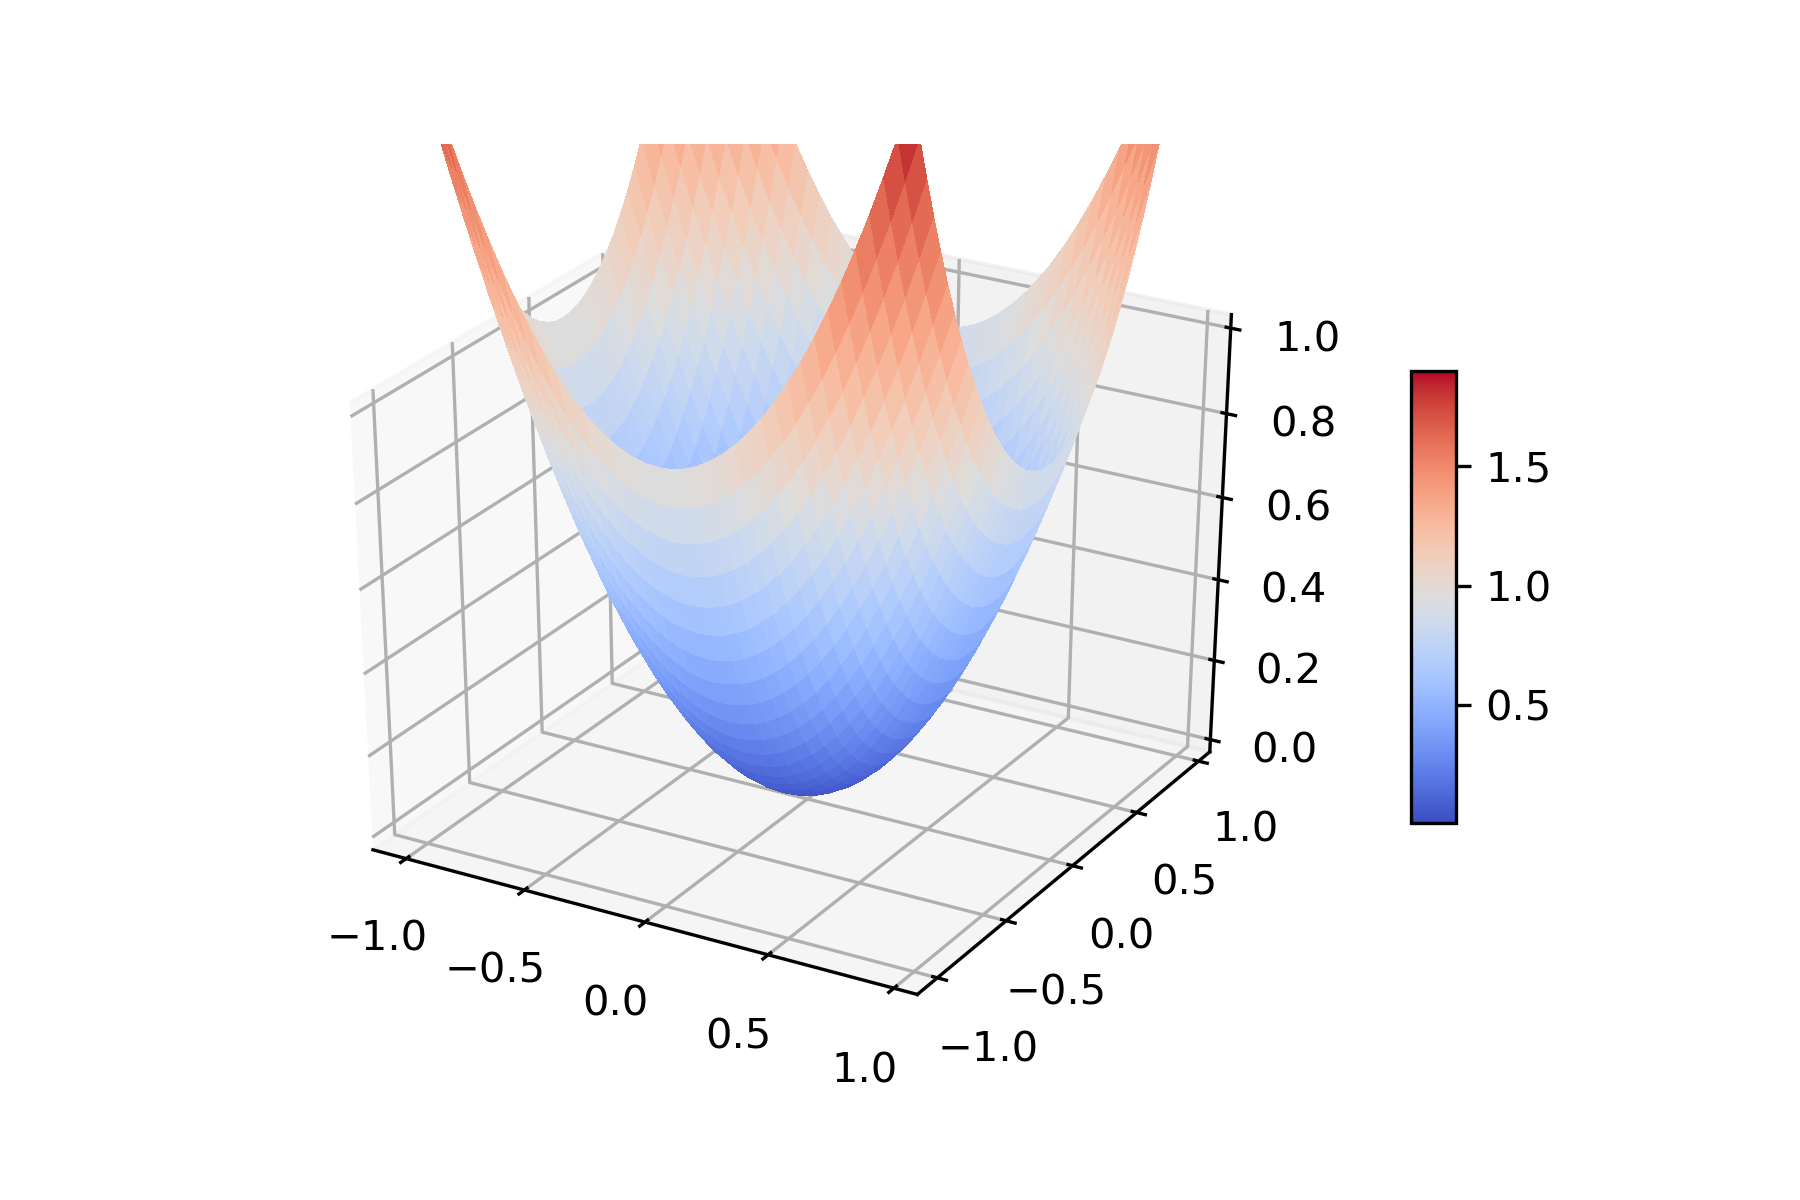
\includegraphics[scale = 0.5]{Figures/graph_positive.png}

\item Отрицательно определенная форма $z = - x^2 - y^2$.
Начало координат -- точка максимума.

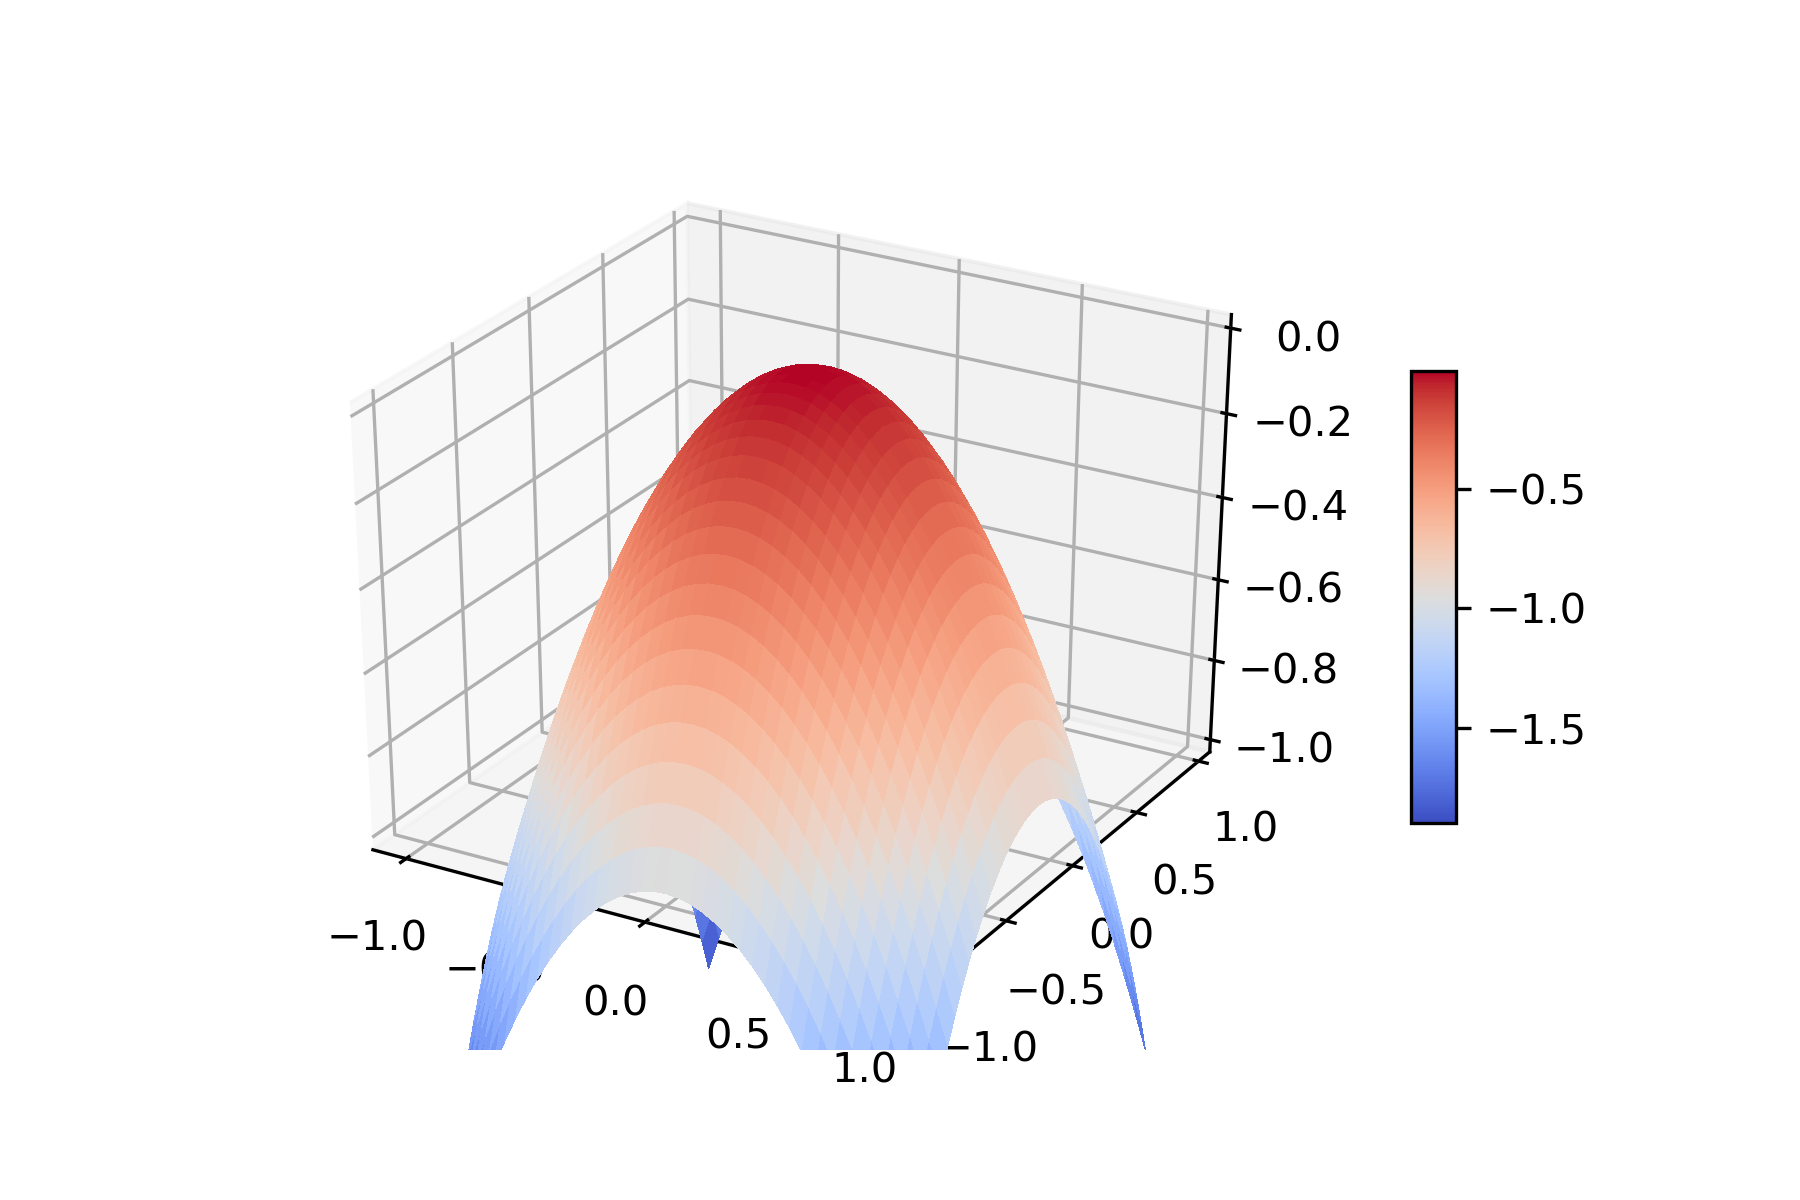
\includegraphics[scale = 0.5]{Figures/graph_negative.png}

\item Неотрицательно определенная форма $z = x^2$.
Минимум достигается на прямой $ x = 0$.

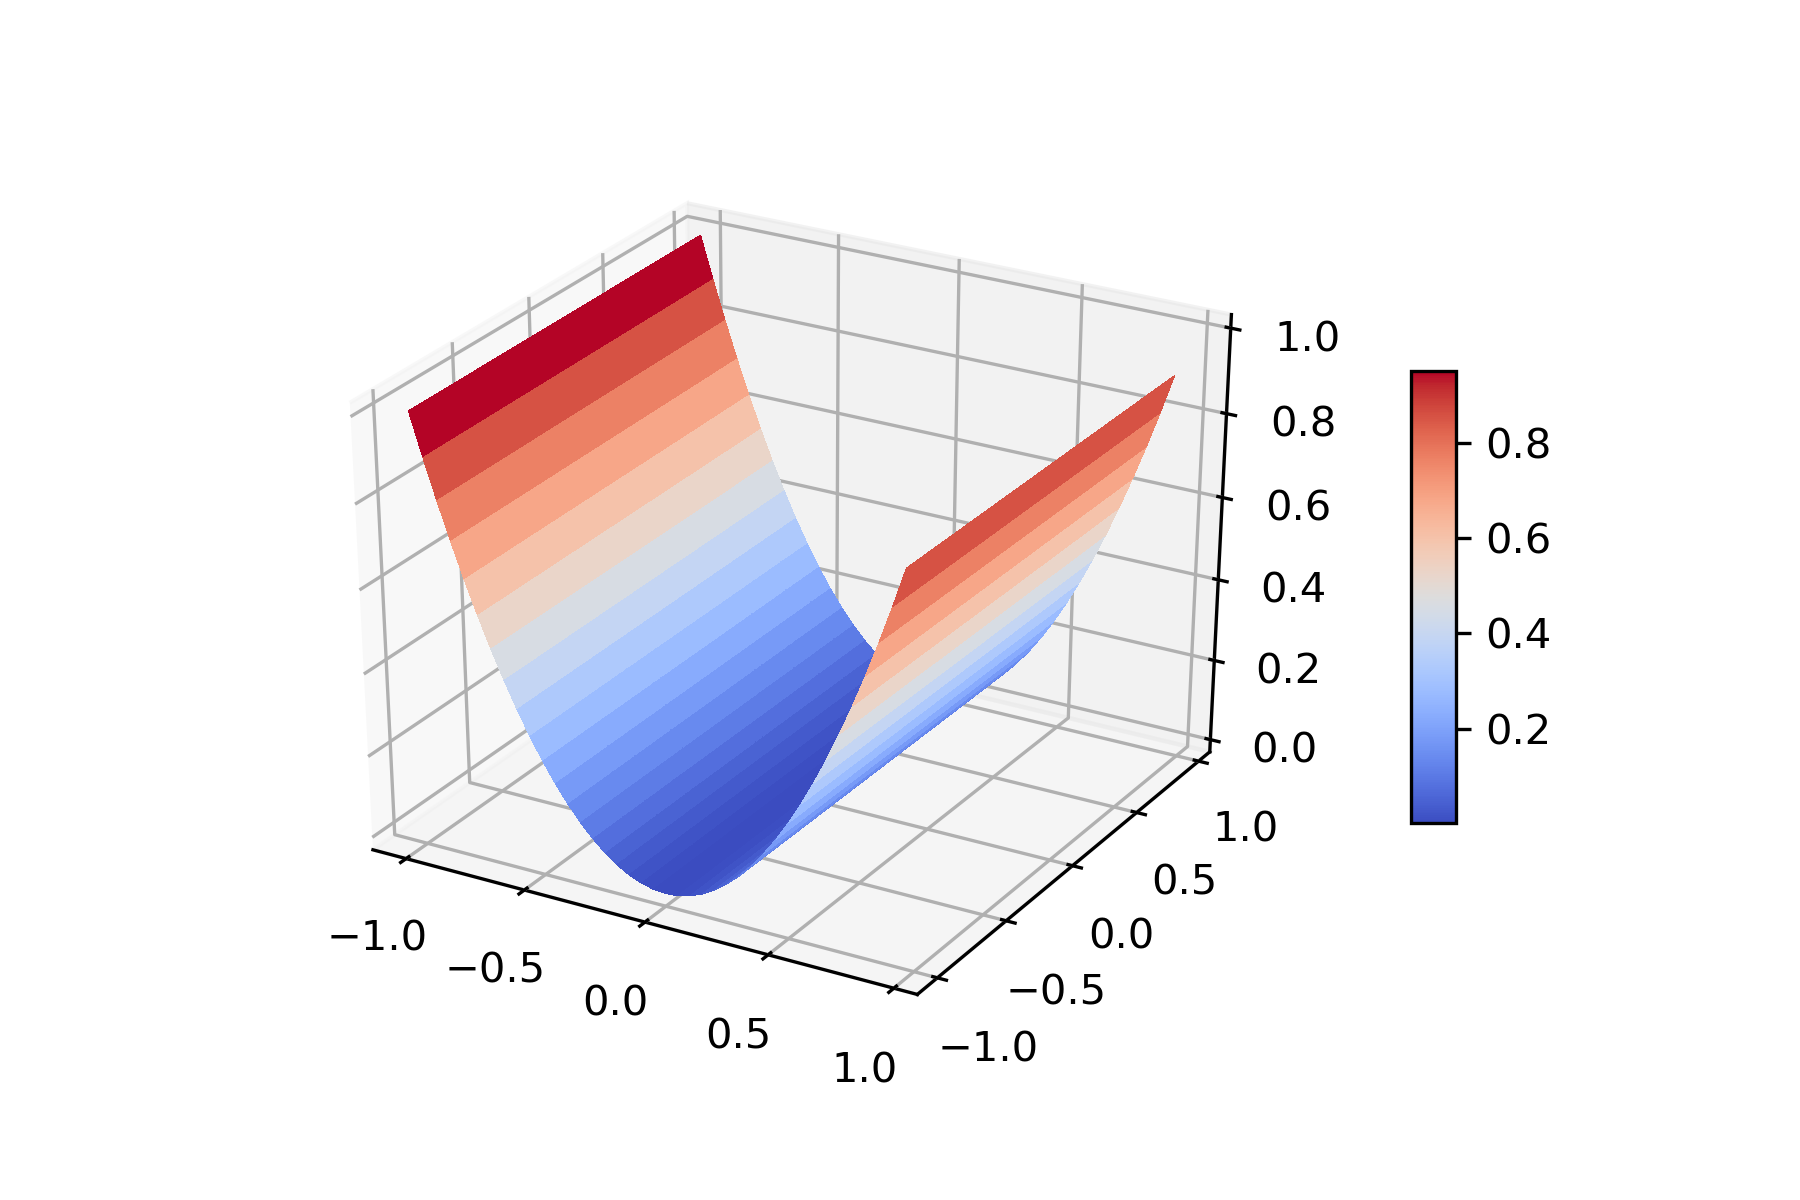
\includegraphics[scale = 0.5]{Figures/graph_non_negative.png}

\item Неположительно определенная форма $z = - x^2$.
Максимум достигается на прямой $x = 0$.

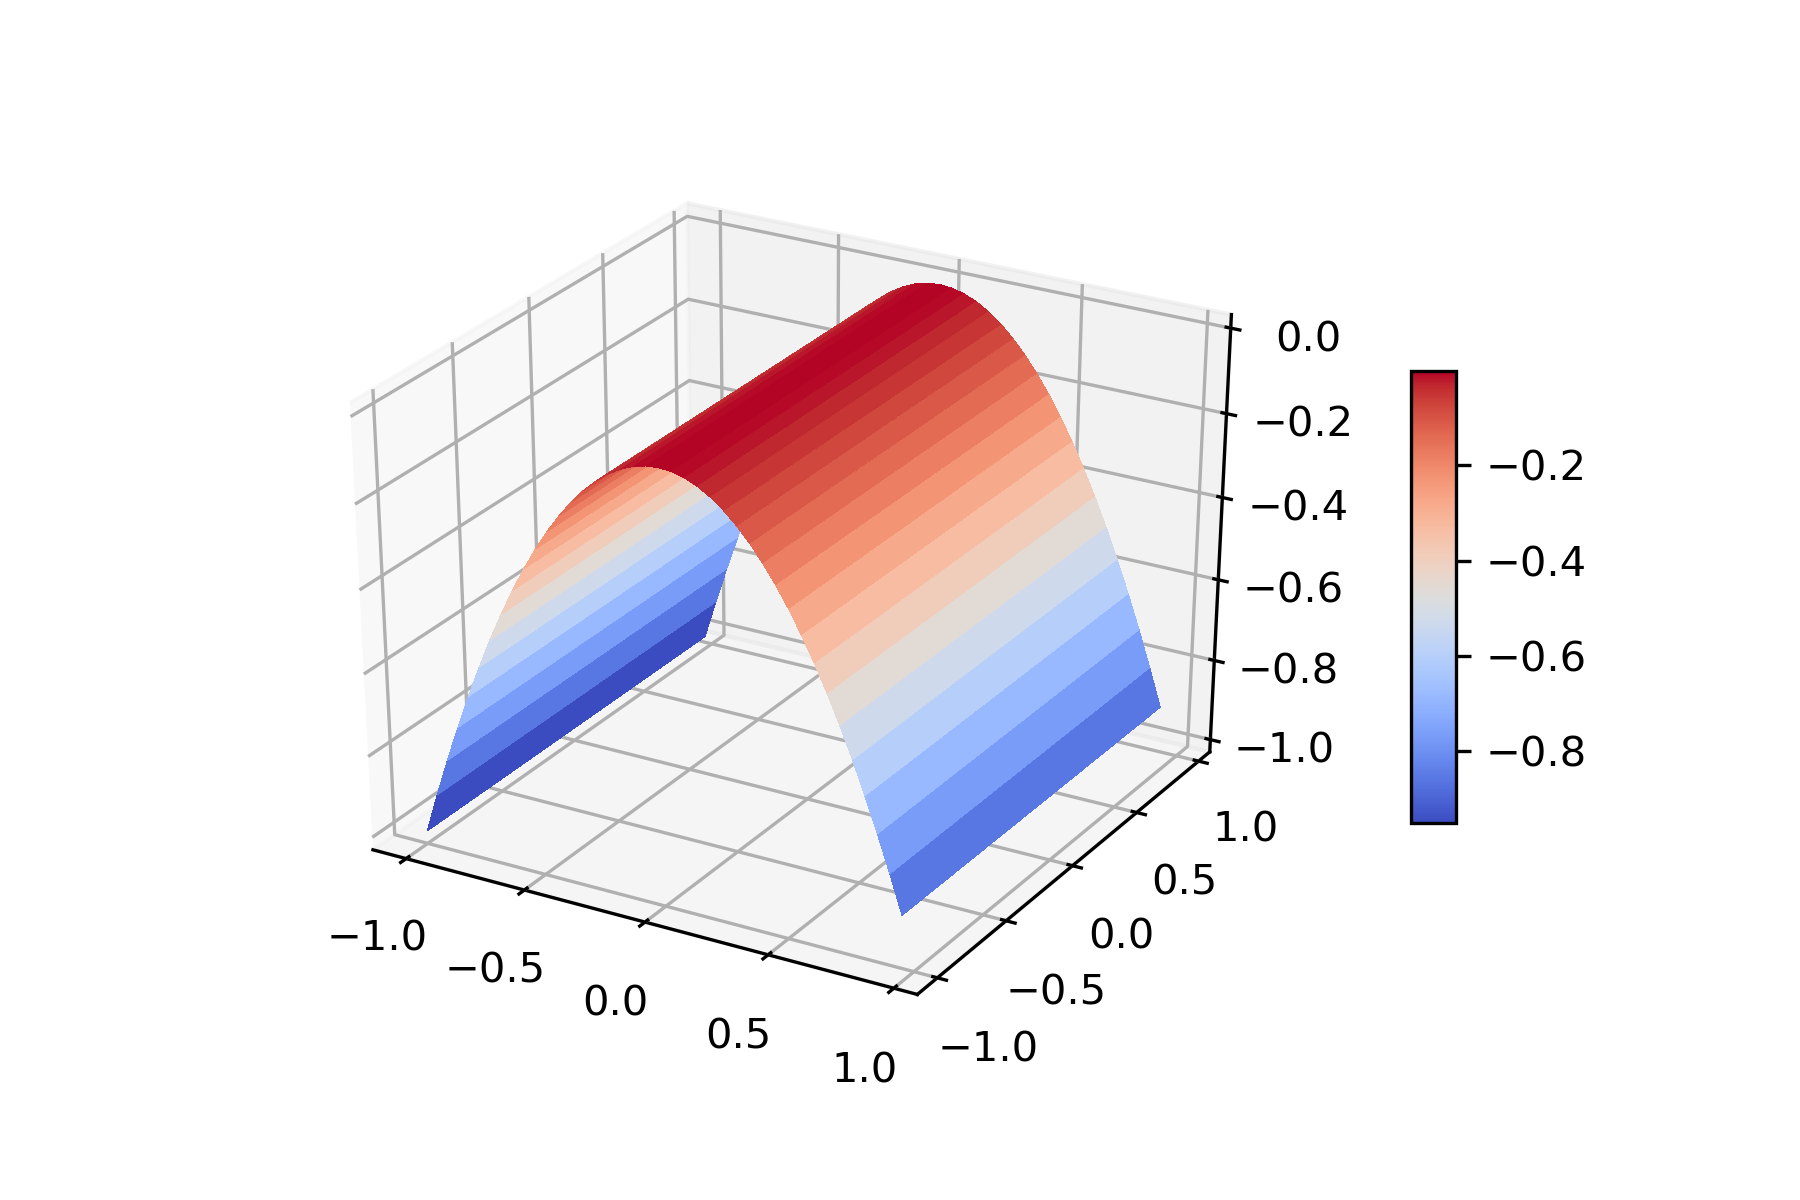
\includegraphics[scale = 0.5]{Figures/graph_non_positive.png}

\item Неопределенная форма $z = x^2 - y^2$.
Начало координат -- седловая точка.

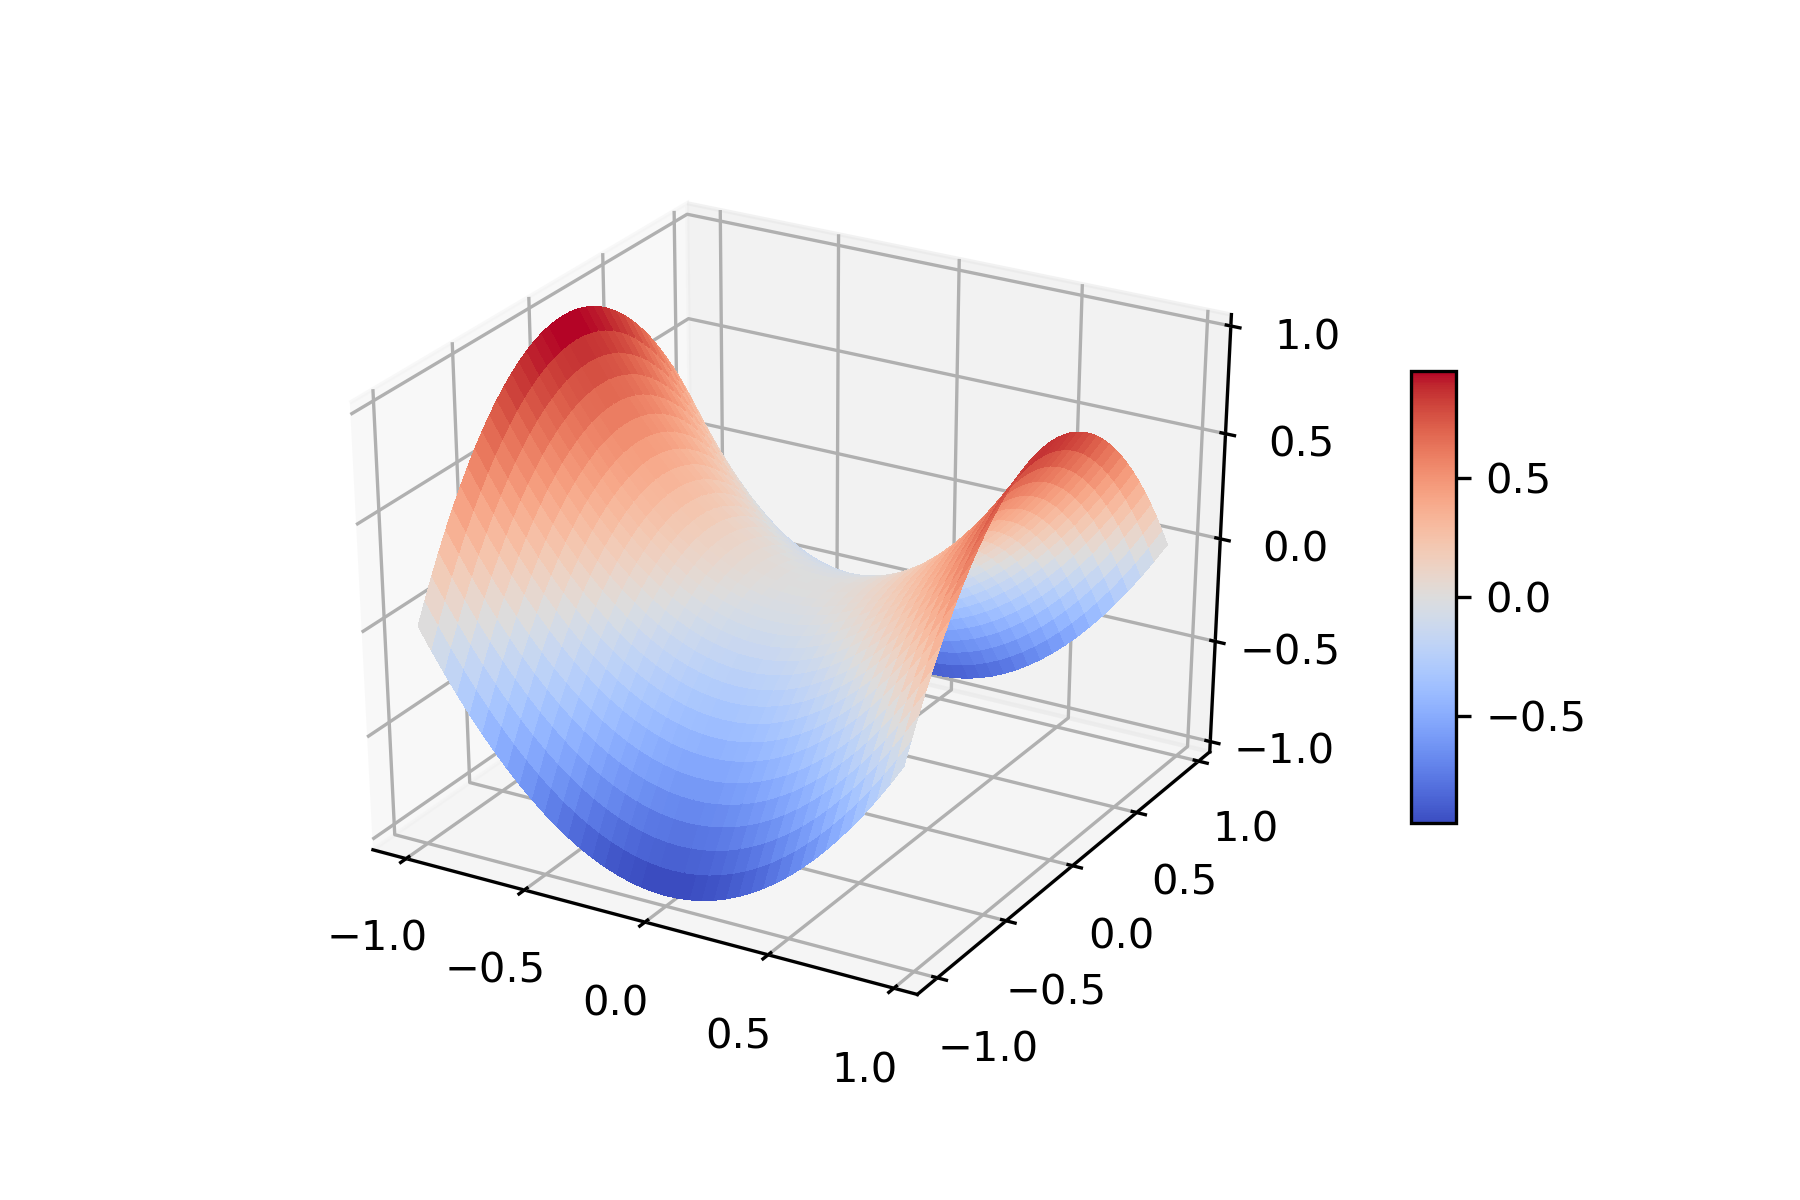
\includegraphics[scale = 0.5]{Figures/graph_saddle.png}
\end{enumerate}


\subsection{Анализ поверхности}

Квадратичные формы применяются для анализа поверхности графика функции от многих переменных.
Давайте я вкратце обрисую как.
Пусть $f\in C^2(\mathbb R^n)$ -- функция $n$ переменных, дифференцируемая дважды и вторые производные все непрерывны.
Тогда для любой точки $a\in \mathbb R^n$ выполнено разложение Тейлора
\[
f(z) = f(a) + \sum_{i=1}^n \frac{\partial f}{\partial x_i}(a)(z_i-a_i) + \sum_{ij=1}^n\frac{\partial^2 f}{\partial x_i\partial x_j}(a)(z_i-a_i)(z_j-a_j) + o(|z - a|^2)
\]
Здесь $o(|z-a|^2) = |z-a|^2 o(1)$, где $o(1)\to 0$ когда $z \to a$.
Геометрический смысл слагаемых следующий
\begin{enumerate}
\item Первое слагаемое $f(a)$ -- значение функции в точке.
Тут я никого этим не удивил.
Это лучшее приближение константой для нашей функции в точке $a$.

\item Второе слагаемое
\[
\sum_{i=1}^n \frac{\partial f}{\partial x_i}(a)(z_i-a_i)
\]
задает касательную плоскость в точке $a$ к графику функции $y = f(z)$.
То есть это линейное приближение для графика функции.
Эта плоскость горизонтальна тогда и только тогда, когда $ \frac{\partial f}{\partial x_i}(a) = 0$ для всех $1\leqslant i\leqslant n$.

\item Третье слагаемое 
\[
\sum_{ij=1}^n\frac{\partial^2 f}{\partial x_i\partial x_j}(a)(z_i-a_i)(z_j-a_j)
\]
является квадратичным приближением для графика функции.
Матрица с коэффициентами $\frac{\partial^2 f}{\partial x_i\partial x_j}(a)$ задает квадратичную форму называемую гессианом.
Если касательная плоскость горизонтальна, то сигнатура этой квадратичной формы определяет поведение графика в окрестности точки.
\begin{itemize}
\item Если форма положительно определена, то это точка локального минимума.

\item Если форма отрицательно определена, то это точка локального максимума.

\item Если форма не вырождена и неопределена, то это седловая точка
\end{itemize}
\end{enumerate}


\newpage
\section{Евклидовы пространства}

\subsection{Определение и примеры}

\begin{definition}
Евклидово пространство -- это пара $V$ и $({-},{-})$, где 
\begin{itemize}
\item $V$ -- векторное пространство над полем $\mathbb R$.

\item $({-},{-})\colon V\times V\to \mathbb R$ -- билинейная форма
\end{itemize}
При этом выполнены следующие аксиомы:
\begin{enumerate}
\item Форма $({-},{-})$ симметрическая.

\item Форма $({-},{-})$ положительно определена.
\end{enumerate}
Такая билинейная форма называется скалярным произведением.
\end{definition}

Очень часто, для краткости, когда задано евклидово пространство $V, ({-},{-})$, говорят, что $V$ является евклидовым пространством, подразумевая, что на нем есть скалярное произведение.

\paragraph{Примеры}

\begin{enumerate}
\item Пространство $\mathbb R^n$ со стандартным скалярным произведением $(x,y) = x^t y$.
Тогда $Q(x) = x^t x = \sum_{i=1}^n x_i^2 > 0$ при $x\neq 0$.

\item Пространство $\Matrix{n}$ со скалярным произведением $(A, B) = \tr(A^t B)$.
Тогда $Q(A) = \tr(A^t A) = \sum_{i,j=1}^n a_{ij}^2 > 0$ при $A\neq 0$.

\item Пусть $C[0,1]$ -- пространство непрерывных функций на отрезке $[0,1]$ сл скалярным произведением $(f,g) = \int_0^1 f(x) g(x)\,dx$.
Тогда $Q(f) = \int_0^1 f^2(x)\,dx > 0$ при $f \neq 0$.%
\footnote{В силу непрерывности, если $f(x)\neq 0$, то в какой-то окрестности $(x-\delta, x+\delta)$ точки $x$ имеем $|f(y)| > |f(x)| - \varepsilon$.}
\end{enumerate}

Важный вопрос: а как задавать скалярные произведения на некотором пространстве $V$?
Если в $V$ выбрать базис, то оно превратится в $\mathbb R^n$.
Тогда скалярное произведение задается симметричной матрицей $B$ с положительной сигнатурой.
Самый неудобный момент здесь заключается в том, что вообще говоря, глядя на матрицу $B$ не очевидно является ли она положительно определенной или нет.
Для этого надо пользоваться критерием Сильвестра (утверждение~\ref{claim::SilvCrit}).
Оказывается есть способ лучше, его мы обсудим далее.


\subsection{Ортогональные и ортонормированные базисы}

\begin{definition}
Пусть $V$ -- евклидово пространство.
Тогда
\begin{itemize}
\item Набор $v_1,\ldots,v_k\in V$ называется ортогональным, если $(v_i,v_j) = 0$ для всех $i\neq j$.


\item Набор $v_1,\ldots,v_k\in V$ называется ортонормированным, если он ортогонален и $(v_i,v_i) = 1$ для любого $i$.
\end{itemize}
Если $e_1,\ldots,e_n$ -- базис $V$, то он называется ортогональным или ортонормированным базисом, если набор $e_1,\ldots,e_n$ ортогонален или ортонормирован.
\end{definition}

\paragraph{Замечания}

\begin{itemize}
\item Базис является ортогональным тогда и только тогда, когда матрица скалярного произведения в нем диагональная.

\item Базис является ортонормированным тогда и только тогда, когда матрица скалярного произведения в нем единичная.

\item Утверждение~\ref{claim::SBilReal} говорит, что матрицу скалярного произведения всегда можно привести к единичной в некотором базисе.
То есть ортонормированные базисы существуют.

\item Процесс применяемый в методе Якоби (раздел~\ref{subsection::JacobyAlg}) превращает любой базис в ортогональный.%
\footnote{В евклидовых пространствах этот процесс называется процессом ортогонализации Грама-Шмидта.
Определение будет дальше.}
\end{itemize}


\begin{claim}
\label{claim::ScalarDef}
Пусть $V$ -- векторное пространство над $\mathbb R$.
Тогда для любого базиса $e_1,\ldots,e_n$ существует единственное скалярное произведение $({-},{-})$ на $V$ такое, что $e_1,\ldots,e_n$ является ортонормированным базисом.
\end{claim}
\begin{proof}
Зафиксируем базис $e_1,\ldots,e_n$.
Тогда задать билинейную форму -- это все равно, что задать матрицу $B\in \Matrix{n}$ (утверждение~\ref{claim::BilinearMatrices}).
Когда такая матрица $B$ задает скалярное произведение, в котором $e_1,\ldots,e_n$ -- ортонормированный базис?
Тогда и только тогда, когда $B = E$.
\end{proof}

По ортогональным и ортонормированным базисам удобно раскладывать произвольные векторы.

\begin{claim}
Пусть $V$ -- евклидово пространство, $e_1,\ldots,e_n$ -- базис и $v\in V$ -- произвольный вектор.
Тогда
\begin{enumerate}
\item Если $e_1,\ldots,e_n$ ортогональный, то 
\[
v = \frac{(v,e_1)}{(e_1,e_1)}e_1 + \ldots + \frac{(v,e_n)}{(e_n,e_n)} e_n
\]

\item Если $e_1,\ldots,e_n$ ортонормированный, то
\[
v = (v,e_1)e_1+\ldots+(v,e_n)e_n
\]
\end{enumerate}
\end{claim}
\begin{proof}
Вторая формула есть элементарное следствие первой, так как $(e_i,e_i) = 1$ для ортонормированного базиса.
Потому достаточно доказать первую формулу.
Пусть $v = \alpha_1e_1+\ldots+\alpha_n e_n$.
Умножим скалярно левую и правую часть на вектор $e_k$, тогда получим $(v, e_k) = \sum_{i=1}^n \alpha_i(e_i, e_k) = \alpha_k (e_k,e_k)$.
Значит, $\alpha_k = \frac{(v,e_k)}{(e_k,e_k)}$, что и требовалось.
\end{proof}


\begin{claim}
Пусть $A\in \Matrix{n}$.
Тогда следующие условия равносильны
\begin{enumerate}
\item $A^t A = E$.

\item $AA^t = E$.

\item $A^t = A^{-1}$.
\end{enumerate}
\end{claim}
\begin{proof}
Это следует из существования и единственности обратного при наличии левого или правого обратного (утверждение~\ref{claim::InvertibleDiscription}).
\end{proof}

\begin{definition}
Матрица $A\in \Matrix{n}$ называется ортогональной, если выполнено одно из эквивалентных свойств из предыдущего утверждения, например, $A^t A = E$.
\end{definition}

\paragraph{Замечание}

Рассмотрим в $\mathbb R^n$ стандартное скалярное произведение.
Если $A\in\Matrix{n}$, то условие $A^t A = E$ означает, что столбцы матрицы $A$ образуют ортонормированный базис.
Условие $A A^t = E$ означает, что строки матрицы $A$ образуют ортонормированный базис.
Важно понимать, что эти условия эквивалентны.
А именно, если вы возьмете ортонормированный базис в $\mathbb R^n$ и поставите эти векторы в столбцы матрицы $A$, то строки этой матрицы автоматически образуют некий другой ортонормированный базис в $\mathbb R^n$.

\begin{claim}
\label{claim::OrthoBasisDiscrEucl}
Пусть $V$ -- евклидово пространство.
Тогда
\begin{enumerate}
\item Если $e_1,\ldots,e_n$ и $f_1,\ldots,f_n$ -- два ортонормированных базиса, то матрица перехода между ними будет ортогональна.

\item Если $e_1,\ldots,e_n$ -- ортонормированный базис и $C\in \Matrix{n}$ -- ортогональная матрица, то базис $(e_1,\ldots,e_n)C$ будет ортонормированным.
\end{enumerate}
\end{claim}
\begin{proof}
(1) Пусть $(f_1,\ldots,f_n) = (e_1,\ldots,e_n)C$, где $C\in \Matrix{n}$.
Так оба базиса ортонормированные, то матрица скалярного произведения в каждом из этих базисов единичная.
По правилу изменения матрицы билинейной формы при смене базиса получаем $E = C^t E C$.
Значит $C$ ортогональная.

(2) Пусть $(f_1,\ldots,f_n) = (e_1,\ldots,e_n)C$.
В базисе $e_1,\ldots,e_n$ матрица билинейной формы $E$, так как он ортонормированный.
Матрица в базисе $f_1,\ldots,f_n$ будет $C^t E C$.
Так как $C$ ортогональная, то это будет $E$, то есть $f_1,\ldots,f_n$ -- ортонормированный базис.
\end{proof}

Таким образом за переход между ортонормированными базисами отвечают только ортогональные матрицы.

\subsection{Классификация Евклидовых пространств}

Если у нас есть два векторных пространства $V$ и $U$, то они изоморфны (то есть по сути одно и то же векторное пространство, но заданное по-разному) тогда и только тогда, когда у них одинаковые размерности (утверждение~\ref{claim::VectorClassific}).
Теперь мы хотим решить ту же самую задачу для евклидовых пространств -- понять, когда они будут одинаковыми.
Для начала надо объяснить, что значит изоморфизм евклидовых пространств.

\begin{definition}
Пусть $V$ и $U$ -- два евклидовых пространства.
Линейное отображение $\phi\colon V\to U$ называется изоморфизмом евклидовых пространств, если
\begin{enumerate}
\item $\phi$ -- изоморфизм векторных пространств.

\item Для любых $v,u\in V$ выполнено $(v, u) = (\phi(v), \phi(u))$.%
\footnote{Здесь слева скалярное произведение в пространстве $V$, а с права в пространстве $U$.}
\end{enumerate}
При наличии изоморфизма между евклидовыми пространствами $V$ и $U$ они называются изоморфными.
\end{definition}

Второе условие в определении можно выразить коммутативностью следующей диаграммы
\[
\xymatrix@R=6pt@C=40pt{
	{V\times V}\ar[dd]^{\phi\times \phi}\ar[rd]&{}&{(v,u)}\ar@{|->}[dd]\ar@{|->}[rd]&{}\\
	{}&{\mathbb R}&{}&{(v,u) = (\phi(v),\phi(u))}\\
	{U\times U}\ar[ru]&{}&{(\phi(v),\phi(u))}\ar@{|->}[ru]&{}
}
\]
Смысл определения в том, что при изоморфизме не только вектора и операции над ними переходят в соответствующие вектора и операции, но и скалярное произведение на первом пространстве превращается в скалярное произведение на втором после применения измоморфизма.
Значит при таком изоморфизме вся структура евклидова пространства сохраняется, а значит мы считаем, что такие пространства одинаковые, как евклидовы пространства.
Более того, все свойства таких пространств (если они выражены в терминах евклидова пространства) одинаковые и одно можно безболезненно менять на другое, если это удобно.


\begin{claim}
\label{claim::EuclideanIsom}
Два евклидовых пространства $V$ и $U$ изоморфны тогда и только тогда, когда $\dim V = \dim U$.
\end{claim}
\begin{proof}
Ясно, что у изоморфных пространств одинаковая размерность.
Потому надо показать, что из условия $\dim V = \dim U$ найдется изоморфизм, согласованный со скалярным произведением.
Давайте выберем ортонормированный базис $e_1,\ldots,e_n$ в $V$ и ортонормированный базис $f_1,\ldots,f_n$ в $U$.
Тогда построим линейное отображение $\phi\colon V\to U$ отправляющее $e_i\mapsto f_i$ (такое найдется единственное по утверждению~\ref{claim::LinMapExist}).
Если векторы $v,u\in V$ имеют координаты $x,y\in \mathbb R^n$ в базисе $e_1,\ldots,e_n$, то векторы $\phi(v),\phi(u)\in U$ имеют те же самые координаты $x,y$ в базисе $f_1,\ldots,f_n$.
Тогда $(v,u) = x^ty$ и $(\phi(v),\phi(u)) = x^ty$.
\end{proof}

\paragraph{Замечания}

\begin{itemize}
\item Таким образом добавление скалярного произведения к пространству не увеличивает количество не изоморфных векторных пространств.

\item Пространство $\mathbb R^2$ со стандартным скалярным произведением является <<школьной плоскостью>>, которую мы все долго и упорно изучали в курсе геометрии школьной программы.
А пространство $\mathbb R^3$ со стандартным произведением является <<школьным пространством>>.

\item Самым важным с идейной точки зрения является следующее наблюдение, которое вытекает из предыдущего утверждения.
Пусть мы хотим доказать что-то про два вектора $v,u\in V$ в каком-то евклидовом пространстве.
Тогда они обязательно содержатся в каком-то двумерном подпространстве $U\subseteq V$.
Само $U$ тоже является евклидовым вместе с ограничением скалярного произведения с $V$.
Но у нас есть школьная плоскость, которая тоже является двумерным евклидовым пространством.
А значит, это то же самое пространство, что и $U$.
То есть нам достаточно доказать факт для произвольных двух векторов на школьной плоскости.
Получается, что автоматически можно пользоваться результатами школьной геометрии.
Аналогичная идея работает с тремя векторами и сведением задачи к школьной стереометрии.

\item Несмотря на то, что можно пользоваться школьной геометрией, бывает полезно понять, как именно доказывать те или иные утверждения пользуясь формализмами линейной алгебры напрямую.
Потому я буду периодически демонстрировать какие-то вещи в лоб.
\end{itemize}

\ProvidesFile{lecture28.tex}[Лекция 28]


\subsection{Геометрия в Евклидовых пространствах}

\begin{definition}
Пусть $V$ -- евклидово пространство и $v\in V$ -- произвольный вектор.
Определим длину вектора $|v| = \sqrt{(v,v)}$.
\end{definition}

\paragraph{Замечания}

\begin{itemize}
\item Именно для того, чтобы определить длину произвольного вектора, нам нужна положительная определенность в определении скалярного произведения.

\item Обратите внимание, что $|v| = 0$ тогда и только тогда, когда $v = 0$.

\item Если выбрать ортонормированный базис, то $|x| = \sqrt{\sum_{i=1}^n x_i^2}$.
То есть это $|{-}|_2$ норма на $\mathbb R^n$.
На самом деле можно развивать теорию норм на произвольных векторных пространствах, как это делается в функциональном анализе.
\end{itemize}

\begin{claim}
[Неравенство Коши-Буняковского]
Пусть $V$ -- евклидово пространство, $v,u\in V$, тогда $|(v,u)|\leqslant |v| |u|$.
Кроме того, равенство достигается тогда и только тогда, когда $u$ и $v$ лежат на одной прямой.
\end{claim}
\begin{proof}
Так как у нас всего два вектора, можно считать, что $V$ двумерно.
Выберем первый базисный вектор $e_1$ вдоль $v$ (если $v$ нулевой, то выбираем любой), а второй -- любой ортогональный к $e_2$ и длины $1$.
Тогда
\[
v = 
\begin{pmatrix}
{a}\\{0}
\end{pmatrix}
\quad\text{и}\quad
u = 
\begin{pmatrix}
{b}\\{c}
\end{pmatrix}
\]
Тогда $|(v, u)| = |ab|$, а $|v||u| = |a|\sqrt{b^2 + c^2}$.
Доказываемое неравенство превращается в $|ab|\leqslant |a|\sqrt{b^2 + c^2}$, что очевидно.

Давайте проанализируем, когда в нем достигается равенство.
Во-первых, если $a = 0$.
В этом случае $v$ и $u$ лежат на одной прямой.
Если $a \neq 0$, то мы получаем условие $|b| = \sqrt{b^2 + c^2}$, что равносильно тому, что $c = 0$.
В этом случае векторы тоже лежат на одной прямой.
Обратно, если вектры лежат на одной прямой, то $v = \lambda e$ и $u = \mu e$ для некоторого ненулевого вектора $e\in V$.
Тогда $(v,u) = \lambda\mu (e,e)$, а с другой стороны $|v||u| = |\lambda e||\mu e| = |\lambda \mu| |e|^2 = |\lambda \mu|(e,e)$.
\end{proof}

\paragraph{Замечание} 

Хочу обратить внимание на то, что по сути доказательство можно было закончить на первой строчке, где я ссылаюсь  на школьную геометрию.
Вся остальная часть всего лишь доказывала факт из школьной геометрии.
Это было сделано для полноты изложения.
К тому же я продемонстрировал метод последовательного выбора удобных базисных векторов, который часто применяется при решении задач аналитической геометрии.
Подобный метод позволяет упростить разбор общего случая в координатах за счет наличия большого количества нулей в векторах.
В нашем случае ноль был всего один, но это сильно сократило вычисления.

Из неравенства Коши-Буняковского следует, что для любых двух ненулевых векторов $v,u\in V$ верно $-1\leqslant \frac{(v,u)}{|v| |u|}\leqslant 1$.
А значит найдется единственное число $\alpha\in [0,\pi]$ такое, что $\cos \alpha = \frac{(v,u)}{|v| |u|}$.

\begin{definition}
Пусть $V$ -- евклидово пространство и $v,u\in V$ -- два вектора.
Тогда число $\alpha$ такое, что $\cos \alpha = \frac{(v,u)}{|v| |u|}$, называется углом между векторами $v$ и $u$.
Будем этот угол обозначать через $\angle(v, u)$.
\end{definition}

\paragraph{Замечание}

Так как два вектора $v$ и $u$ всегда лежат внутри <<школьной плоскости>>, то определение угла превращается в то самое определение угла, которое дается в школьном курсе геометрии.
Потому от этого угла надо ожидать ровно то же самое поведение, к которому мы привыкли в курсе школьной геометрии.
Просто потому, что это тот же самый угол.


\begin{claim}
[Теорема Пифагора]
\label{claim::Pythagoras}
Пусть $V$ -- евклидово пространство и $v,u\in V$ -- два ортогональных вектора, тогда $|v + u|^2 = |v|^2 + |u|^2$.
\end{claim}
\begin{proof}
Формальное доказательство в этом случае является наиболее простым:
\[
|v+u|^2 = (v+u, v+u) = (v,v) + (v,u)+(u,v) +(u,u) = (v,v) + (u,u) = |v|^2 + |u|^2
\]
Здесь $(v,u)=(u,v) = 0$ из ортогональности $u$ и $v$.
\end{proof}

Процесс, применяемый к базисным векторам в методе Якоби (раздел~\ref{subsection::JacobyAlg}), в случае евклидова пространства называется ортогонализацией Грама-Шмидта.
Единственное отличие -- ортогонализация Грама-Шмидта применяется не только к линейно независимым векторам, а к произвольным системам векторов.

\subsubsection*{Ортогонализация методом Грама-Шмидта}

\paragraph{Дано}

Евклидово пространство $V$, система векторов $\{v_1,\ldots,v_k\}\subseteq V$.%
\footnote{Обратите внимание, что $V$ не обязательно задано как пространство столбцов $\Vector{n}$.
Это может быть и пространство многочленов определенной степени или пространство тригонометрических функций, или вообще что угодно.
Даже если $V$ задано как $\Vector{n}$, то скалярное произведение не обязательно стандартное, т.е. скалярное произведение может быть задано любой положительной симметрической матрицей.}

\paragraph{Задача}

Найти систему ортогональных векторов $\{u_1,\ldots,u_r\}\subseteq V$ такую, что $\langle v_1,\ldots,v_k\rangle = \langle u_1,\ldots,u_r\rangle$.

\paragraph{Алгоритм}

\begin{enumerate}
\item В качестве первого вектора $u_1$ берем первый ненулевой вектор из $v_i$.
Если таких нет, то ответ -- пустое множество.

\item Пусть мы нашли вектора $u_1,\ldots,u_s$ и пусть $v_d$ -- первый еще не просмотренный вектор среди $v_i$.
Посчитать вектор 
\[
u' = v_d - \frac{(v_d, u_1)}{(u_1,u_1)} u_1 - \ldots - \frac{(v_d, u_s)}{(u_s, u_s)}u_s
\]

\item Если $u' \neq 0$ положим $u_{s+1} = u'$, иначе пропустим $v_d$.
Теперь перейдем к предыдущему шагу с вектором $v_{d+1}$ вместо $v_d$.
\end{enumerate}


\subsection{Проекции}

\begin{claim}
Пусть $V$ -- евклидово пространство и $U\subseteq V$ -- произвольное подпространство.
Тогда $V = U\oplus U^\bot$.
\end{claim}
\begin{proof}
Это в точности утверждение~\ref{claim::NonDegRestrictionBil} пункт~(2).
\end{proof}

Таким образом в евклидовом пространстве $V$ при фиксированном подпространстве $U\subseteq V$, любой вектор $v\in V$ единственным образом раскладывается в сумму $v = \pr_U v + \ort_U v$, где $\pr_U v \in U$ и $\ort_U v\in U^\bot$.


\begin{definition}
Если $V$ -- евклидово пространство, $U\subseteq V$ -- произвольное подпространство и $v\in V$, то 
\begin{itemize}
\item Вектор $\pr_U v$ называется ортогональной проекцией $v$ на $U$.

\item Вектор $\ort_U v$ называется ортогональной составляющей $v$ относительно $U$.
\end{itemize}
\end{definition}

Обратите внимание, что ортогональная проекция $v$ на $U$ -- это проекция $v$ на $U$ вдоль $U^\bot$, а ортогональная составляющая -- проекция $v$ на $U^\bot$ вдоль $U$.

\subsubsection*{Формула БАБА}

Давайте я в начале разберу задачу нахождения проекции вектора на подпространство вдоль другого подпространства (здесь нам не нужно никакое скалярное произведение).
Пусть $V$ -- некоторое векторное пространство и $V = U\oplus W$.
Тогда на пространстве $V$ задан оператор проекции $P\colon V\to V$ такой, что $\ker P = W$ и $P|_U = \Identity$, то есть, если $v\in V$ раскладывается в сумму $v = u + w$, где $u\in U$ и $w\in W$, то $Pv = u$ -- оператор вычисления проекции на $U$ вдоль $W$.


Теперь мы хотим научиться эффективно считать $P$.
Для этого предположим $V = \mathbb R^n$, $U = \langle u_1,\ldots,u_k\rangle$, $W = \{y\in \mathbb R^n\mid Ay = 0\}$, где $A\in \MatrixDim{s}{n}$.
В этом случае $P\colon \mathbb R^n\to \mathbb R^n$ задается некоторой матрицей.
Наша задача -- найти эту матрицу.

Предположим для простоты, что векторы $u_1,\ldots,u_k$ образуют базис $U$, а строки матрицы $A$ линейно независимы.
Определим матрицу $B = (u_1|\ldots|u_k)\in \MatrixDim{n}{k}$.
Тогда утверждаются следующие вещи:
\begin{enumerate}
\item Количество столбцов $B$ совпадает с количеством строк $A$, то есть $k = s$.

\item Матрица $AB$ обратима.

\item Оператор проекции задается формулой $P = B(AB)^{-1}A$.
Мнемоническое правило <<БАБА>>.
\end{enumerate}
\begin{proof}
Так как мы уже взрослые, я позволю себе пользоваться линейными операторами и отображениями, а не просто матричной техникой.
Матрица $A$ задает линейное отображение $A\colon \mathbb R^n \to \mathbb R^s$ такое, что $\ker A = W$ и $\Im A = \mathbb R^s$ (так как строки матрицы $A$ линейно независимы, то $\rk A = s$, но $\rk A = \dim \Im A$).
Матрица $B$ задает отображение $B\colon \mathbb R^k \to \mathbb R^n$ такое, что $\Im B = U$ и $\ker B = 0$ (так как столбцы $B$ линейно независимы).

(1) Теперь мы знаем, что 
\[
\begin{aligned}
\dim U + \dim W = n\\
\dim \ker A + \dim \Im A = n
\end{aligned}
\quad\text{ то есть }\quad
\begin{aligned}
k + \dim W = n\\
\dim W+ s= n
\end{aligned}
\quad\text{ откуда }\quad
s = k
\]

(2) Теперь рассмотрим отображение $AB\colon \mathbb R^k \to \mathbb R^k$.
Заметим, что $\Im B \cap \ker A = U \cap W = 0$.
Значит $\ker AB = 0$, то есть $AB$ -- обратимый оператор.

(3) Теперь выведем формулу для $P$.
Пусть $v = u + w$, где $v\in \mathbb R^n$ -- произвольный вектор, $u\in U$ и $w\in W$ -- его единственное разложение по прямой сумме подпространств.
Тогда $Av = Au + Aw = Au$.
С другой стороны, так как $u\in U$, мы имеем $u = B x$ для некоторого $x\in \mathbb R^k$.
Тогда $Av = ABx$.
Так как $AB$ обратимая квадратная матрица, имеем $x = (AB)^{-1}Av$.
Значит $u = Bx = B(AB)^{-1}Av$, что и требовалось.
\end{proof}

Обратите внимание, что проектор $P$ на $U$ вдоль $W$ зависит от двух подпространств, а не только от $U$.
Если вы измените одно из них, то проектор изменится.

\subsubsection*{Формула Атата}

Пусть $V = \mathbb R^n$ со стандартным скалярным произведением $(x, y) = x^ty$ и пусть подпространство $U\subseteq V$ задано своим базисом $U = \langle u_1,\ldots,u_k\rangle$.
Составим матрицу $A = (u_1|\ldots|u_k)\in\MatrixDim{n}{k}$.
Тогда $U^\bot = \{y\in \mathbb R^n \mid A^t y = 0\}$.
Пусть теперь $v\in V$ -- произвольный вектор и $v = \pr_U v + \ort_U v$.
Тогда формула <<БАБА>> превращается в $\pr_U v = A(A^tA)^{-1}A^tv$.
Мнемоническое правило для запоминания: в евклидовом пространстве БАБА -- это Атата.

Обратите внимание, что проектор $P$ всегда зависит от двух подпространств: то, на которое проектируем $U$, и то, вдоль которого проектируем $W$.
Но в случае ортогонального проектирования $W = U^\bot$, потому ортопроектор $P$ реально зависит только от одного подпространства.

\subsection{Расстояния и углы}

\begin{definition}
Пусть $V$ -- евклидово пространство и $u,v\in V$ -- произвольные векторы.
Тогда определим расстояние между векторами по формуле $\rho(u,v) = |u - v|$.
\end{definition}

\begin{claim}
Расстояние $\rho$ на евклидовом пространстве $V$ удовлетворяет следующим свойствам:
\begin{enumerate}
\item {\bf Невырожденность} $\rho(v,u) \geqslant 0$ для любых $u,v\in V$ причем равенство достигается тогда и только тогда, когда $v = u$.

\item {\bf Симметричность} $\rho(u,v) = \rho(v,u)$ для любых $u,v\in V$.

\item {\bf Неравенство треугольника} $\rho(u,v)\leqslant \rho(u,w) + \rho(w,v)$ для любых $u,v,w\in V$.
\end{enumerate}
\end{claim}
\begin{proof}
(1) По определению $\rho(v,u) = |v-u| \geqslant 0$ причем равенство достигается тогда и только тогда, когда $v - u = 0$.

(2) По определению $\rho(v, u) = |v - u| = |u-v| = \rho(u,v)$.

(3) Нам надо доказать $\rho(u,v)\leqslant \rho(u,w) + \rho(w,v)$, то есть $|u-v|\leqslant |u-w| + |w - v|$.
Положим $x = u - w$ и $y = w - v$.
Тогда нам надо доказать $|x + y|\leqslant |x| + |y|$.
Так как левая и правая части этого неравенства неотрицательные, то оно равносильно неравенству $|x+y|^2\leqslant (|x| + |y|)^2$.
Проверяем:
\[
|x+y|^2 = (x+y, x+y) = (x, x) + 2(x, y) + (y,y) = |x|^2 + 2 (x, y) + |y|^2
\]
По неравенству Коши-Буняковского $(x, y)\leqslant |x| |y|$.
Значит
\[
|x|^2 + 2 (x, y) + |y|^2\leqslant |x|^2 + 2|x||y| + |y|^2= (|x|+|y|)^2
\]
\end{proof}

\paragraph{Замечание}

Если на множестве $X$ задана функция $\rho\colon X\times X\to \mathbb R$ со свойствами из предыдущего утверждения, то пара $(X,\rho)$ называется метрическим пространством.
Самое главное, что известно про метрические пространства -- принцип сжимающих отображений.
Это один из способов доказывать существование объектов с  нужными свойствами.
Есть два важных примера:
\begin{itemize}
\item Теорема о неявной функции.
Ее доказательство через принцип сжимающих отображений в разы проще и доступнее, чем копание в координатах.

\item Теорема о существовании и единственности решения дифференциального уравнения.
Дифференциальное уравнение обычно заменяется на интегральное, после чего можно пользоваться метрическими пространствами и принципом сжимающих отображений.
\end{itemize}
В нашем случае метрика на евклидовом пространстве скорее является случайным гостем, заглянувшем на огонек, нежели чем-то фундаментальным и сверх полезным.
Самым полезным является понимание роли метрических пространств.

\begin{definition}
Пусть $X,Y\subseteq V$ -- произвольные подмножества евклидова пространства, тогда расстояние между ними определяется следующим образом:
\[
\rho(X, Y) = \inf_{\substack{x\in X\\y\in Y}}\rho(x, y)
\]
\end{definition}
Обратите внимание, что это расстояние не удовлетворяет аксиоме не вырожденности, то есть расстояние между разными множествами может быть нулевым.
Например, для этого достаточно, чтобы $X$ и $Y$ имели непустое пересечение.
Но, даже если $X\cap Y = \varnothing$, расстояние может быть нулем.
Например, если $X, Y \subseteq \mathbb R$ и $X = \{\frac{1}{n}\mid n\in \mathbb N\}$ и $Y = - X = \{-\frac{1}{n}\mid n\in \mathbb N\}$.

\begin{definition}
Пусть $V$ -- евклидово пространство, $v\in V$ и $L\subseteq V$ -- некоторое подпространство.
Тогда углом между $v$ и $L$ называется $\angle (v, L) = \inf_{u\in L}\angle (v,u)$.
\end{definition}

Теперь давайте обсудим, как эффективно находить некоторые расстояния и углы.

\begin{claim}
\label{claim::DistAngle}
Пусть $V$ -- евклидово пространство, $L\subseteq V$ -- подпространство, $v\in V$ -- некоторый вектор.
Тогда
\begin{enumerate}
\item $\rho(v, L) = |\ort_L v|$.

\item $\angle(v, L) = \angle(v, \pr_L v)$.%
\footnote{Если $\pr_L v = 0$, то надо считать косинус угла нулевым, то есть угол равным $\pi/2$.}
\end{enumerate}
\end{claim}
\begin{proof}
(1) Пусть $u\in L$ -- произвольный вектор отличный от $\pr_L v$.
Достаточно показать, что 
\[
\rho(v, u) > \rho (v, \pr_Lv) = |v - \pr_Lv| = |\ort_L v|
\]
Рассмотрим треугольник образованный концами следующих трех векторов: $v$, $\pr_Lv$, $u$.
Сторона $v - \pr_Lv = \ort_L v$ ортогональна стороне $u - \pr_L v \in L$.
Значит $u - v$ -- гипотенуза прямоугольного треугольника.Тогда по теорема Пифагора (утверждение~\ref{claim::Pythagoras})
\[
\rho(v,u) = |u - v| = \sqrt{|\ort_Lv|^2 + |u - \pr_Lv|^2 }> |\ort_Lv|
\]
Последнее неравенство строгое, так как $u\neq \pr_Lv$.

(2) В начале рассмотрим случай $\pr_L v = 0$.
Это значит, что вектор $v$ ортогонален $L$ и угол с любым вектором $\pi/2$.
Теперь предположим, что $\pr_L v \neq 0$.
Выберем произвольный вектор $u\in L$ отличный от $\pr_L v$ и имеющий такую же длину, как $\pr_L v$.
Тогда рассмотрим два треугольника: первый на векторах $0$, $v$, $\pr_Lv$, второй $0$, $v$, $u$.
Тогда у обоих треугольников стороны при вершине $0$ попарно одинаковой длины, а противоположные стороны -- $\ort_L v$ и $u - v$ соответственно.
Но по доказанному выше $|\ort_L v| < |u - v|$.
А школьная геометрия учит нас, что в этом случае угол в первом треугольнике меньше, чем во втором.

\paragraph{формальное доказательство}

Для любителей формализма я приготовил второе доказательство.
Случай $\pr_L v = 0$ разбирается так же как и выше.
Случай $\ort_L v = 0$ означает, что $v\in L$.
В этом случае угол между вектором и пространством нулевой и минимум достигается на $u = v$.
Теперь считаем, что $\pr_L v \neq 0$, $\ort_L v \neq 0$ и выберем произвольный вектор $u\in L$ такой, что $|u| = |\pr_L v|$.
Теперь выберем единичный вектор $e_1$ пропорциональный $\pr_L v$.
Выберем единичный вектор $e_2$ в плоскости $\langle \pr_Lv, u\rangle$ ортогональным $e_1$.
Единичный вектор $e_3$ выберем  пропорциональным $\ort_L v$.
Тогда все интересные нам векторы живут в пространстве $\langle e_1,e_2,e_3\rangle$.
Давайте запишем их в этом базисе
\[
v = 
\begin{pmatrix}
{\lambda}\\{0}\\{\mu}
\end{pmatrix},\quad
\pr_Lv = 
\begin{pmatrix}
{\lambda}\\{0}\\{0}
\end{pmatrix},\quad
u = 
\begin{pmatrix}
{a}\\{b}\\{0}
\end{pmatrix},\quad
\text{причем}\quad
\lambda^2 = a^2 + b^2,\;\lambda > 0
\]
Условие $v = \pr_Lv$ означает $b = 0$ и $\lambda = a$.
Нам надо показать, что $\angle (v, \pr_L v) < \angle (v, u)$.
То есть $\cos \angle (v, \pr_L v) > \cos \angle (v, u)$.
То есть надо показать, что 
\[
\frac{(v, \pr_L v)}{|v||\pr_L v|} > \frac{(v, u)}{|v||u|}
\]
Но так как $|u| = |\pr_Lv|$ по выбору, нам надо доказать, что $(v, \pr_L v) > (v, u)$, то есть, что $\lambda^2 > \lambda a$.
Из условия $\lambda^2 = a^2 + b^2$ видно, что $|\lambda| > |a|$ при $b \neq 0$.
Значит $\lambda^2 > |\lambda a|$ при $b \neq 0$.
При $b = 0$ имеем $a = \lambda$ либо $a = -\lambda$.
Если $u \neq \pr_L v$, то возможно только $a = -\lambda$, но тогда неравенство очевидно.
\end{proof}

\paragraph{Замечания}

\begin{itemize}
\item Обратите внимание, что угол между вектором и подпространством всегда находится в интервале $[0, \pi/2]$ или что то же самое косинус угла всегда неотрицательный.

\item Заметим следующую связь $\angle (v, \pr_L v) + \angle (v, \ort_L v) = \pi/2$.
Причем формула верна даже когда проекция или ортогональная составляющая равны нулю.
В этом случае соответствующий угол надо считать равным $\pi/2$.

\item Предположим, что подпространство $L\subseteq V$ имеет коразмерность $1$, то есть $\dim L = \dim V - 1$.
Тогда у нас $L^\bot$ -- одномерно.
Пусть $n\in L^\bot$ какой-нибудь ненулевой вектор.
Таким образом $n$ -- вектор нормали к $L$.
В этом случае $n$ лежит с $\ort_L v$ на одной прямой (может быть сонаправлен ему или смотреть в противоположную сторону).
Тогда $\angle (v, \ort_L v)$ равен либо $\angle (v, n)$ либо $\angle (v, - n)$ (на самом деле не большему из этих двух).
То есть в этом случае можно взять к $L$ произвольную нормаль $n$, посчитать угол $\alpha$.
Если он оказался больше $\pi/2$ заменить его на $\pi - \alpha$.
После чего найти угол с подпространством как $\pi/2$ минус полученный угол.
\end{itemize}

\input{Lectures/lecture29}
\ProvidesFile{lecture30.tex}[Лекция 30]


\begin{definition}
Пусть $V$ -- евклидово пространство с фиксированной ориентацией.
Тогда определим ориентированный $n$-мерный объем следующим образом.
Пусть $(v_1,\ldots,v_n)\in V$, тогда
\[
\Vol^{or}_n\Pi(v_1,\ldots,v_n) = 
\left\{
\begin{aligned}
0&,& &v_1,\ldots,v_n\text{ линейно зависимы}\\
\Vol_n\Pi(v_1,\ldots,v_n)&,& &(v_1,\ldots,v_n)\text{ положительно ориентирован}\\
-\Vol_n\Pi(v_1,\ldots,v_n)&,& &(v_1,\ldots,v_n)\text{ отрицательно ориентирован}
\end{aligned}
\right.
\]
\end{definition}


\begin{claim}
Пусть $V$ -- евклидово пространство размерности $n$ с фиксированной ориентацией, $(v_1,\ldots,v_n)\in V^n$ и $C\in \Matrix{n}$.
Тогда
\[
\Vol^{or}_n\Pi((v_1,\ldots,v_n)C) = \det C \Vol^{or}_n\Pi(v_1,\ldots,v_n)
\]
\end{claim}
\begin{proof}
Если матрица $C$ вырождена, то набор векторов $(v_1,\ldots,v_n)C$ линейно зависим, а значит левый объем равен  нулю.
С другой стороны $\det C = 0$, а значит и правая часть равна нулю.
Аналогично, если $(v_1,\ldots,v_n)$ линейно зависимый набор, то и набор $(v_1,\ldots,v_n)C$ тоже линейно зависим.
А тогда объемы в левой и правой частях равны нулю.
Осталось разобраться со случаем $(v_1,\ldots, v_n)$ -- базис и $C$ -- невырожденная матрица.
В этом случае совпадение левой и правой части по модулю следует из утверждения~\ref{claim::Volume} об изменении объемов при линейной замене образующих параллелепипеда.
Осталось проверить, что у них совпадают знаки.
Если $\det C > 0$, то наборы $(v_1,\ldots,v_n)$ и $(v_1,\ldots, v_n)C$ одинаково ориентированы.
Значит знаки у $\Vol^{or}_n\Pi((v_1,\ldots, v_n)C) $ и $\Vol^{or}_n \Pi((v_1,\ldots, v_n))$ одинаковые, а к тому же $\det C > 0$.
Значит знаки обеих частей равны.
Пусть теперь $\det C < 0$.
Тогда знаки у $\Vol^{or}_n\Pi((v_1,\ldots, v_n)C) $ и $\Vol^{or}_n \Pi((v_1,\ldots, v_n))$ разные.
Но при этом $\det C < 0$, что делает знаки левой и правой части одинаковыми.
Победа!
\end{proof}

\paragraph{Пример}

Пусть $V = \mathbb R^n$ со стандартным скалярным произведением $(x, y) = x^t y$.
И пусть ориентация зафиксирована так, что стандартный базис является положительным.
Возьмем $v_1,\ldots,v_n\in \mathbb R^n$ произвольный набор векторов.
Образуем матрицу $A = (v_1|\ldots|v_n)\in \Matrix{n}$.
Тогда 
\begin{itemize}
\item $G(v_1,\ldots,v_n) = A^t A$.

\item $\det G(v_1,\ldots,v_n) = \det A^2$.

\item $\Vol_n\Pi(v_1,\ldots,v_n) = |\det A|$.

\item $\Vol^{or}_n\Pi(v_1,\ldots,v_n) = \det A$.
\end{itemize}
Заметьте, что ориентация набора (как и знак соответствующего объема) меняется при перестановке векторов в наборе на знак совершенной перестановки.
Другая причина знака объема -- смена направления вектора, то есть когда вектор $v_i$ в наборе меняется на вектор $-v_i$.

\begin{claim}
Пусть $V$ -- ориентированное евклидово пространство размерности $n$, $v_1,\ldots,v_n\in V$ -- некоторый набор векторов и $\varphi\colon V\to V$ -- линейный оператор.
Тогда 
\[
\Vol^{or}_n(\varphi(\Pi(v_1,\ldots,v_n))) = \det \varphi \Vol^{or}_n(\Pi(v_1,\ldots,v_n))
\]
\end{claim}
\begin{proof}
Выберем положительно ориентированный ортонормированный базис $e_1,\ldots,e_n$.
Тогда $V$ превращается в $\mathbb R^n$, скалярное произведение становится стандартным $(x, y) = x^t y$, линейное отображение превращается в умножение на матрицу $\varphi(x) = Cx$, а векторы $v_1,\ldots,v_n$ расставим по столбцам матрицы $A = (v_1|\ldots|v_n)$.

Как мы видели в предыдущем примере
\[
\Vol^{or}_n(\Pi(v_1,\ldots,v_n)) = \det A,\quad
\Vol^{or}_n(\varphi(\Pi(v_1,\ldots,v_n))) = \det CA
\]
А так как $\det C = \det \varphi$ по определению, утверждение вытекает из мультипликативности определителя.
\end{proof}


\newpage
\section{Комплексные векторные пространства}

В начале несколько общих слов о том, зачем все это надо и куда оно нас заведет.
Этот раздел будет полностью посвящен векторным пространствам над полем $\mathbb C$.
Основная задача этого поля -- помогать решать трудности поля $\mathbb R$.
Но для этого нам надо уметь заменять вещественные объекты комплексными.
Например, вещественное векторное пространство превращать в комплексное векторное пространство.
Беда с евклидовыми пространствами в том, что среди билинейных форм над $\mathbb C$ нет аналога скалярного произведения.
Потому приходится от билинейных форм переходить к так называемым полуторалинейным.
Оказывается, что в этом случае можно построить полноценный аналог евклидовых пространств в комплексном мире, такие пространства называются эрмитовыми (но я иногда буду их называть евклидовыми над $\mathbb C$, чтобы подчеркнуть аналогию).
Кроме этого я покажу как переходить от вещественных объектов к комплексным и наоборот.
Мы будем менять пространства, операторы, билинейные формы и прочее.
Основная идея будет уследить за тем, как при подобных заменах меняются характеристики этих объектов.
Этому будет посвящен раздел комплексификации и овеществления.

\subsection{Полуторалинейные формы}

\begin{definition}
Пусть $V$ -- векторное пространство над полем $\mathbb C$, отображение $\beta \colon V\times V\to \mathbb C$ называется полуторалинейным, если выполнены следующие свойства:
\begin{enumerate}
\item $\beta(v_1+v_2, u) = \beta(v_1,u) + \beta(v_2, u)$, для любых $v_1, v_2, u\in V$

\item $\beta(\lambda v, u) = \bar \lambda \beta(v, u)$, для любых $v, u \in V$ и $\lambda\in \mathbb C$.

\item $\beta(v, u_1 + u_2) = \beta(v, u_1) + \beta(v, u_2)$, для любых $v, u_1, u_2\in V$.

\item $\beta(v, \lambda u) = \lambda\beta(v, u)$, для любых $v,u \in V$ и $\lambda \in \mathbb C$.
\end{enumerate}
\end{definition}

В этом случае говорят, что $\beta$ полулинейна по первому аргументу и линейна по второму.
Обратите внимание, что выбор первого аргумента для полулинейности является случайным и в разной литературе принято по-разному определять полуторалинейность.
В одних источниках полулинейность в первом аргументе, в других -- во втором.

\begin{definition}
Пусть $V$ -- векторное пространство над $\mathbb C$.
Множество всех полуторалинейных форм на пространстве $V$ я буду обозначать через $\Bil_{1\frac{1}{2}}(V)$.
Это множество является векторным пространством над $\mathbb C$ относительно операций:
\[
(\beta_1+\beta_2)(v, u) := \beta_1(v,u) + \beta_2(v,u)\quad\text{и}\quad (\lambda\beta)(v,u) = \lambda\beta(v,u),\quad\text{где}\quad v,u\in V,\;\lambda\in \mathbb C
\]
\end{definition}

Для удобства введем следующее техническое определение.
\begin{definition}
Пусть $A\in \operatorname{M}_{m\,n}(\mathbb C)$, тогда определим матрицу $\bar A$ как матрицу, в которой мы применили сопряжение ко всем элементам матрицы $A$, то есть $(\bar A)_{ij} = \overline{A_{ij}}$.
Кроме того, определим $A^* = \bar A^t$ и будем называть матрицу $A^*$ эрмитово сопряженной к матрице $A$.%
\footnote{Вообще говоря, правильный подход к определению матрицы $A^*$ следующий.
В случае вещественного поля надо положить $A^* = A^t$, а в случае комплексного $A^* = \bar A^t$.
Тогда у нас одно обозначение и надо лишь упоминать в каком мире мы живем -- комплексном или вещественном.
Я предпочитаю единую технику, которая работает в разных ситуациях, чем иметь миллион разных способов под каждую конкретную задачу.}
\end{definition}

Как обычно начинаем с конструкторов и правил, как работать с новыми объектами.

\begin{claim}
Пусть $V$ -- векторное пространство над $\mathbb C$ и $\beta \colon V\times V \to \mathbb C$ -- полуторалинейная форма.
Тогда
\begin{enumerate}
\item Для любого базиса $e_1,\ldots,e_n\in V$ определим матрицу $B$ с коэффициентами $\beta(e_i, e_j)$.
Тогда в координатах базиса $e_1,\ldots,e_n$ полуторалинейная форма записывается в виде $\beta(x, y) = \bar x^t B y$.

\item Если $(e'_1,\ldots,e'_n) = (e_1,\ldots,e_n)C$ -- некоторый другой базис, в котором матрица полуторалинейной формы есть $B'$ с коэффициентами $\beta(e'_i,e'_j)$, то $B' = \bar C^t B C = C^* B C$.

\item Для любого фиксированного базиса $e_1,\ldots,e_n\in V$ отображение $\Bil_{1\frac{1}{2}}(V)\to \operatorname{M}_n(\mathbb C)$ сопоставляющее полуторалинейной форме $\beta$ ее матрицу $B = (\beta(e_i,e_j))$ является изоморфизмом векторных пространств.
\end{enumerate}
\end{claim}
\begin{proof}
(1) Если $e = (e_1,\ldots,e_n)$ -- базис в $V$ и $v,u\in V$, тогда $v = ex$ и $u = ey$, где $x,y\in \mathbb C^n$.
В этом случае
\[
\beta(v,u) = \beta(\sum_i x_i e_i, \sum_j y_j e_j) = \sum_{ij}\bar x_i y_j \beta(e_i, e_j) = \bar x^t B y
\]

(2) Пусть в этом случае $v,u\in V$ и при этом $v = ex = e' x'$ и $u = ey = e'y'$, где $x,y,x',y'\in \mathbb C^n$.
Тогда по формулам замены координат вектора (формулы в конце раздела~\ref{subsection::FnSpace}) $x = Cx'$ и $y = Cy'$.
Тогда
\[
\beta(v,u) =\beta(x,y) = \bar x^t B y = \overline{Cx'}^t B C y' = (\bar x')^t \bar C^t B C y' = \beta(x',y') = (\bar x')^t B' y'
\]
Значит $B' = \bar C^t B C = C^* B C$.

(3) Линейность правила $\beta\mapsto B = (\beta(e_i, e_j))$ проверяется непосредственно.
Также непосредственно проверяется, что правило $B\mapsto \beta(x,y) = \bar x^t B y$ линейно и задает обратное отображение.
Я оставлю эту рутину на радость читателю.
\end{proof}


\subsection{Сведение к билинейным формам}
Теперь нам хотелось бы обобщить на случай полуторалинейных форм все те факты, что мы доказали для билинейных форм.
Есть два пути: мучительный и долгий, когда мы по аналогии с билинейными формами все доказываем заново, или мучительный и быстрый, когда мы вводим некую неприятную абстракцию, которая объяснит, как свести полуторалинейные формы к билинейным.
Я считаю, что если уж и мучиться, то лучше по-быстрому, и пойду вторым путем.

\begin{definition}
Пусть $V$ -- векторное пространство над $\mathbb C$.
Определим новое векторное пространство $\bar V$ следующим образом.
Как множество $\bar V = V$.
Теперь на нем надо задать операции сложения и умножения на скаляр.
Сложение зададим так же, как оно было задано на $V$.
А умножение определим по формуле $\lambda *v = \bar \lambda v$, где справа стоит исходная операция умножения на скаляр в $V$.
\end{definition}

Обратите внимание, что пространства $V$ и $\bar V$ имеют одинаковую размерность.
Более того, набор векторов $e_1,\ldots,e_n$ является базисом в $V$ тогда и только тогда, когда он является базисом в $\bar V$.

\paragraph{Пример}

Пусть $V = \mathbb C^n$, тогда в пространстве $\bar V$ операции заданы следующим образом
\[
\begin{pmatrix}
{x_1}\\{\vdots}\\{x_n}
\end{pmatrix}
+
\begin{pmatrix}
{y_1}\\{\vdots}\\{y_n}
\end{pmatrix}
=
\begin{pmatrix}
{x_1 + y_1}\\{\vdots}\\{x_n + y_n}
\end{pmatrix}
\quad\text{и}\quad
\lambda
\begin{pmatrix}
{x_1}\\{\vdots}\\{x_n}
\end{pmatrix}
=
\begin{pmatrix}
{\bar \lambda x_1}\\{\vdots}\\{\bar \lambda x_n}
\end{pmatrix}
\]

\paragraph{Замечания}

\begin{itemize}
\item Пусть $\beta\colon V\times V\to \mathbb C$ -- полуторалинейная форма, тогда на нее можно посмотреть как на отображение $\beta\colon \bar V\times V\to \mathbb C$ в этом случае $\beta$ становится билинейной формой.
И наоборот если $\beta\colon \bar V\times V\to \mathbb C$ билинейная форма, то $\beta\colon V\times V\to \mathbb C$ -- полуторалинейная форма.
Таким образом можно пользоваться всеми фактами про билинейные формы, смотря на полуторалинейную форму, как на отображение $\beta\colon \bar V\times V\to \mathbb C$.

\item Заметим, что подмножество $U\subseteq V$ является подпространством в $V$ тогда и только тогда, когда оно является подпространством в $\bar V$.
То есть запас подпространств в $V$ и $\bar V$ одинаковый.
\end{itemize}

\begin{definition}
Пусть $\beta\colon V\times V\to \mathbb C$ -- полуторалинейная форма.
Тогда
\begin{itemize}
\item Для любого подпространства $W\subseteq V$ определим его левое и правое ортогональное дополнение как левое и правое ортогональное дополнение для соответствующей билинейной формы, то есть:
\[
W^\bot = \{v\in V\mid \beta(W,v) = 0\}\quad \text{и} \quad {}^\bot W = \{v\in V\mid \beta(v, W) = 0\}
\]

\item  определим ее левое и правое ядра, как левые и правые ядра соответствующей билинейной формы $\beta\colon \bar V\times V\to \mathbb C$, то есть $\ker^L \beta= {}^\bot V$ и $\ker^R \beta = V^\bot$.

\item Полуторалинейная форма $\beta$ будет называться невырожденной, если соответствующая билинейная форма невырождена.
То есть когда $\ker^L\beta = \ker ^R\beta = 0$.%
\footnote{Так как $\dim \bar V = \dim V$, то это условие равносильно тому, что одно из ядер равно нулю.}
Это равносильно тому, что матрица $B = (\beta(e_i, e_j))$ формы в любом базисе $e_1,\ldots,e_n$ невырождена.
\end{itemize}
 
\end{definition}

\begin{claim}
Пусть $V$ -- векторное пространство над $\mathbb C$ и $\beta \colon V\times V\to \mathbb C$ -- невырожденная полуторалинейная форма.
Тогда
\begin{enumerate}
\item Для любого подпространства $W\subseteq V$ выполнено
\[
\dim W^\bot + \dim W = \dim V
\]

\item Для любого подпространства $W\subseteq V$ выполнено ${}^\bot(W^\bot) = W$.

\item Для любых подпространств $W\subseteq E\subseteq V$ верно, что $W^\bot \supseteq E^\bot$.
Причем $W = E$ тогда и только тогда, когда $W^\bot = E^\bot$.

\item Для любых подпространств $W, E\subseteq V$ выполнено равенство
\[
(W + E)^\bot = W^\bot \cap E^\bot
\]

\item Для любых подпространств $W, E\subseteq V$ выполнено равенство
\[
(W\cap E)^\bot = W^\bot + E^\bot
\]
\end{enumerate}
Аналогичные свойства выполняются для левых ортогональных дополнений ${}^\bot W$.
\end{claim}
\begin{proof}
Это следует из двойственности для подпространств для билинейных форм (утверждение~\ref{claim::DualitySpaces}) и предыдущего замечания.
\end{proof}

\subsection{Квадратичные формы}


\begin{definition}
Пусть $\beta\colon V\times V\to \mathbb C$ -- полутора линейная форма.
Тогда $Q_\beta\colon V\to \mathbb C$ по правилу $v\mapsto \beta(v,v)$ называется квадратичной формой.%
\footnote{Мы можем рассматривать полуторалинейную форму $\beta$, как билинейную форму $\beta\colon \bar V\times V\to \mathbb C$.
Но билинейная форма получается на разных пространствах, потому у нас нет понятия квадратичной формы для $\beta$, как для билинейной формы.
Потому введенное определение квадратичной формы не должно вызвать путаницы.}
\end{definition}

\paragraph{Замечания}

\begin{itemize}
\item Если $e_1,\ldots,e_n\in V$ -- некоторый базис, в котором полуторалинейная форма задается в виде $\beta(x, y) = \bar x^t B y$, то соответствующая ей квадратичная форма имеет вид $Q_\beta(x) = \bar x^t B x$.
Множество квадратичных форм для полуторалинейных форм на пространстве $V$ будем обозначать через $\Quad_{1\frac{1}{2}}(V)$.%
\footnote{Индекс в виде $1\frac{1}{2}$ нужен, чтобы отличить, мы строим квадратичные формы по билинейным или полуторалинейным.}

\item Ключевое свойство квадратичных форм $Q\colon V\to \mathbb C$ заключается в следующем: для любого $v\in V$ и любого $\lambda\in \mathbb C$ выполнено $Q(\lambda v) = |\lambda|^2Q(v)$.
\end{itemize}

Главное отличие от билинейных форм -- любая полуторалинейная форма (без каких-либо дополнительных требований) восстанавливается по своей квадратичной форме.
Давайте разберемся почему это так.

\begin{claim}
[Поляризационная формула]
\label{claim::CPolarization}
Пусть $\beta\colon V\times V\to \mathbb C$ -- произвольная полуторалинейная форма и $Q_\beta\colon V\to \mathbb C$ -- соответствующая ей квадратичная форма.
Тогда 
\[
\beta(v, u) = \sum_{k=0}^3 \frac{i^k}{4}Q_\beta\left(i^k v + u\right) = \frac{Q_\beta(v+u) + iQ_\beta(iv+u) - Q_\beta(-v + u) -i Q_\beta(-iv+u)}{4}
\]
\end{claim}
\begin{proof}
Рассмотрим следующее выражение
\begin{gather*}
\beta(v + u, v+ u) + i\beta(iv + u, iv+ u) - \beta(-v + u, -v+ u) -i \beta(-iv + u, -iv+ u)=\\
\beta(v,v)+\beta(v,u)+\beta(u,v)+\beta(u,u)+\\
+i\beta(v,v)+\beta(v,u)-\beta(u,v)+i\beta(u,u)-\\
-\beta(v,v)+\beta(v,u)+\beta(u,v)-\beta(u,u)-\\
-i\beta(v,v)+\beta(v,u)-\beta(u,v)-i\beta(u,u)=\\
4 \beta(v, u)
\end{gather*}
Разделив обе части на $4$, получаем требуемое.
\end{proof}

\paragraph{Замечание}

В частности, если $\beta(v, v) = 0$ для любого вектора $v\in V$, то полуторалинейная форма $\beta$ тождественно равна нулю.

\begin{claim}
\label{claim::CBilQuad}
Пусть $V$ векторное пространство над $\mathbb C$, тогда отображения
\begin{itemize}
\item $\phi\colon\Bil_{1\frac{1}{2}}(V)\to \Quad_{1\frac{1}{2}}(V)$ по правилу $\beta\mapsto Q_\beta(v) = \beta(v,v)$ (в координатах $\bar x^t B y$ переходит в $\bar x^t B x$)

\item $\psi\colon\Quad_{1\frac{1}{2}}(V)\to \Bil_{1\frac{1}{2}}(V)$ по поляризационной формуле $Q\mapsto \beta_Q(v,u) = \sum_{k=0}^3 \frac{i^k}{4}Q(i^k v + u)$ (в координатах $\bar x^t A x$ переходит в $\bar x^t A y$)
\end{itemize}
являются взаимно обратными изоморфизмами.
\end{claim}
\begin{proof}
По определению, отображение $\phi$ сюръективно.
Из поляризационной формулы (утверждение~\ref{claim::CPolarization}) следует, что композиция $\psi\phi$ равна тождественному отображению.
А значит $\phi$ инъективно, то есть биекция.
При этом $\psi$ является левым обратным к обратимому отображению, а значит просто обратным.
Получили, что $\phi$ и $\psi$ взаимнообратные биекции.
Тот факт, что они изоморфизмы, то есть линейны, непосредственно следует из определения.
\end{proof}

\paragraph{Замечания}

\begin{itemize}
\item Последнее утверждение означает, что полуторалинейные формы и квадратичные формы -- это одно и то же.
В частности, матрица $A$ в определении квадратичной формы однозначно определена.
Действительно, если $Q(x) = \bar x^t A x$ в координатах, то ей соответствует билинейная форма $\beta_Q(x, y) = \bar x^t A y$.
Матрица билинейной формы $A$ определена правилом $a_{ij} = \beta_Q(e_i, e_j)$.

\item Для любопытных, давайте в лоб проверим, что $\phi\psi = \Identity$.
Пусть $Q\colon V\to \mathbb C$ -- произвольная квадратичная форма, тогда она переходит в
\begin{gather*}
\frac{Q(v+v) + iQ(iv+v) - Q(-v+v) -i Q(-iv + v)}{4} = \frac{Q(2v) + iQ((1+i)v) - i Q((1-i)v) - Q(0)}{4} =\\ =\frac{|2|^2 Q(v)+i|1+i|^2Q(v) - i|1-i|^2Q(v)}{4} = Q(v)
\end{gather*}
\end{itemize}

\subsection{Эрмитовы и косоэрмитовы формы}

Так исторически сложилось, что аналоги симметричных и кососимметричных полуторалинейных форм не принято называть симметричными и кососимметричными (как бы мне этого ни хотелось), у них есть другие более пристойные (с точки зрения математического сообщества) названия.
Однако, очень важно понимать, что мы сейчас будем заниматься не чем иным, как изучением аналогов симметричных  и кососимметричных форм, потому и все результаты будут очень ожидаемыми.

\begin{definition}
Пусть $\beta\colon V\times V\to \mathbb C$ -- полуторалинейная форма.
Тогда 
\begin{itemize}
\item $\beta$ называется эрмитовой если $\beta(v, u) = \overline{\beta(u,v)}$ для любых $v,u\in V$.
Это аналог симметричных форм.

\item $\beta$ называется косоэрмитовой, если $\beta(v, u) = -\overline{\beta(u,v)}$ для любых $v,u\in V$.
Это аналог кососимметричных форм.
\end{itemize}
\end{definition}

\paragraph{Замечания}

\begin{itemize}
\item Обратите внимание, что множество эрмитовых (или косоэрмитовых) форм НЕ является векторным пространством над $\mathbb C$, но является векторным пространством над $\mathbb R$.
Действительно, если $\beta(v, u) = \overline{\beta(u,v)}$ для любых $v, u \in V$ и $\lambda\in \mathbb C$, то форма $\lambda \beta$ уже не обязательно эрмитова.
Например, если $\lambda = i$, то $\overline{i\beta(v,u)} = -i \beta(u,v)$.
Как видно из этого вычисления, эрмитова форма после умножения на $i$ превращается в косоэрмитову и наоборот.
В этом смысле изучение эрмитовых или косоэрмитовых форм -- это одно и то же.

\item Правильно думать про эрмитовы и косоэрмитовы формы, как про аналоги вещественной и мнимой части (только мнимая часть рассматривается вместе с мнимой единицей).
В данном случае аналогом комплексного сопряжения является операция $\beta(v,u) \mapsto \overline{\beta(u, v)}$.
Тогда неподвижная часть будет аналогом вещественной части, а меняющая знак -- аналогом мнимой домноженной на $i$.
При этом любая полуторалинейная форма представляется единственным способом в виде суммы эрмитовой и косоэрмитовой:
\[
\beta(v,u) = \frac{\beta(v, u) + \overline{\beta(u, v)}}{2} + \frac{\beta(v, u) - \overline{\beta(u, v)}}{2} 
\]
Или в матричной форме
\[
B = \frac{B + B^*}{2} + \frac{B - B^*}{2}
\]
\end{itemize}

\begin{claim}
\label{claim::CSymBil}
Пусть $\beta\colon V\times V\to \mathbb C$ -- полуторалинейная форма.
Тогда
\begin{enumerate}
\item Пусть $e_1,\ldots,e_n$ -- некоторый базис и $B$ -- матриц полуторалинейной формы в этом базисе.
\begin{itemize}
\item Форма $\beta$ эрмитова тогда и только тогда, когда $B^* = B$.

\item Форма $\beta$ косоэрмитова тогда и только тогда, когда $B^* = - B$.
\end{itemize}

\item Форма $\beta$ эрмитова тогда и только тогда, когда $Q_\beta(v) = \beta(v,v)\in\mathbb R$ для любого $v\in V$.

\item Если форма $\beta$ эрмитова или косоэрмитова, то для любого подпространства $W\subseteq V$ верно $W^\bot = {}^\bot W$.
\end{enumerate}
\end{claim}
\begin{proof}
(1) Пусть после выбора базиса в координатах форма имеет вид $\beta(x, y) = \bar x^t B y$.
Тогда эрмитовость равносильна свойству
\[
\bar x^t B y = \overline{\bar y^t B x} = y^t \bar B \bar x = (y^t \bar B \bar x)^t = \bar x^t \bar B^t y = \bar x^t B^* y
\]
Так как это свойство выполнено для любых $x,y\in \mathbb C^n$, то $B = B^*$.
Аналогично показывается для косоэрмитовых форм.

(2) $\Rightarrow$ Пусть $\beta$ эрмитова.
Тогда $\beta(v,v) = \overline{\beta(v,v)}$.
То есть $Q_\beta(v) = \beta(v,v)\in \mathbb R$.

$\Leftarrow$ Наоборот, применим поляризационную формулу, тогда
\begin{gather*}
\beta(v,u) = \frac{Q(v+u) + iQ(iv+u) - Q(-v+u) - iQ(-iv+u)}{4}=\\
\frac{Q(v+u) + iQ(i(v-iu)) - Q(-(v-u)) - iQ(-i(v+iu))}{4}=\\
\frac{Q(v+u) + i|i|^2Q(v-iu) -|-1|^2 Q(v-u) - i|-i|^2Q(v+iu)}{4}=\\
\frac{Q(v+u) + iQ(v-iu) - Q(v-u) - iQ(v+iu)}{4}
\end{gather*}
Если $Q(v)\in \mathbb R$ для любого $v\in V$, то последнее выражение есть
\[
\overline{\frac{Q(v+u) - iQ(v-iu) - Q(v-u) + iQ(v+iu)}{4}} = \overline{\beta(u,v)}
\]
То есть форма эрмитова.

(3) Для эрмитовых форм по определению получаем
\[
W^\bot = \{v\in V\mid \beta(W, v) = 0\} = \{v\in V\mid \overline{\beta(v, W)} = 0\} = \{v\in V\mid \beta(v, W) = 0\} = {}^\bot W
\]
Аналогично для косоэрмитовых.
\end{proof}

\paragraph{Замечание}

Обратите внимание, что в случае полуторалинейных форм, отличительной особенностью эрмитовых является тот факт, что соответствующая им квадратичная форма принимает только вещественные значения.
Именно это явление и позволяет нам проводить с ними те же самые трюки, которые работали с симметричными билинейными формами над полем $\mathbb R$.


\begin{claim}
Пусть $V$ -- векторное пространство над $\mathbb C$ и $\beta\colon V\times V\to \mathbb C$ -- полуторалинейная форма.
Тогда
\begin{enumerate}
\item Если форма $\beta$ эрмитова, то существует базис $e_1,\ldots,e_n$ такой, что матрица формы $B_\beta$ диагональная с вещественными числами на диагонали.

\item Если форма $\beta$ косоэрмитова, то существует базис $e_1,\ldots,e_n$ такой, что матрица формы $B_\beta$ диагональная с чисто мнимыми числами на диагонали.
\end{enumerate}
\end{claim}
\begin{proof}
(1)$\Rightarrow$(2) Если форма $\beta$ косоэрмитова, то $i\beta$ будет эрмитова.
Тогда в каком-то базисе матрица формы $i\beta$ будет диагональна с вещественными числами на диагонали.
То есть матрица формы $\beta$ диагональная с чисто мнимыми числами на диагонали.

(1) Так как на диагонали у эрмитовой формы всегда находятся вещественные числа (утверждение~\ref{claim::CSymBil} пункт~(2)), то достаточно показать, что матрица формы диагонализуется.
Поступать будем так же, как и в случае билинейных форм.
Рассмотрим квадратичную форму $Q_\beta(v)$.
Если она тождественно равна нулю, то $\beta$ тоже тождественно равна нулю (утверждение~\ref{claim::CBilQuad}).
Тогда матрица нулевая и доказывать нечего.
Пусть теперь $v$ -- такой вектор, что $\beta(v,v) = Q_\beta(v) \neq 0$.
Это значит, что $v\notin \langle v\rangle^\bot$, то есть $\langle v\rangle \cap \langle v\rangle^\bot = 0$.
По определению $\langle v\rangle^\bot = \ker \beta(v, {-})$ является ядром ненулевого линейного функционала, то есть имеет размерность $\dim V - 1$.
Значит $V = \langle v\rangle\oplus \langle v\rangle^\bot$.
Теперь берем вектор $v$ в качестве первого базисного вектора $e_1$.
Индукцией по размерности пространства находим ортогональный базис $e_2,\ldots,e_n$ в $\langle v\rangle^\bot$ для формы $\beta|_{\langle v\rangle^\bot}$.
Победа!
\end{proof}

\ProvidesFile{lecture31.tex}[Лекция 31]


\begin{claim}
Пусть $V$ -- векторное пространство над $\mathbb C$ и $\beta\colon V\times V\to\mathbb C$ -- эрмитова форма.
Тогда существует базис, в котором матрица формы имеет вид
\[
B_\beta = 
\begin{pmatrix}
{E}&{}&{}\\
{}&{-E}&{}\\
{}&{}&{0}\\
\end{pmatrix}
\]
При этом количество единиц, минус единиц и нулей на диагонали не зависит от базиса.
\end{claim}
\begin{proof}
Мы уже знаем, что эрмитова форма в некотором базисе диагонализуется.
То есть существует базис, что $\beta(x, y) = \sum_{i=1}^n d_i \bar x_i y_i$, где $d_i\in \mathbb R$.
Перестановкой базисных элементов будем считать, что сначала идут все положительные коэффициенты, потом отрицательные и только потом нулевые, то есть $\beta(x,y) = \sum_{i=1}^k d_i \bar x_i y_i - \sum_{i=k+1}^r d_i \bar x_i y_i$, где все $d_i > 0$.
В этом случае сделаем замену $x_i' = \sqrt{d_i}x_i$.
Получим $\beta(x_i',y_i') = \sum_{i=1}^k \bar x_i' y_i' - \sum_{i=k+1}^r \bar x_i' y_i'$.
А значит, можно привести к такому виду.


Теперь покажем единственность.
Количество единиц и минус единиц вместе дает ранг матрицы.
А ранг матрицы билинейной формы $\beta\colon \bar V\times V\to \mathbb C$ не меняется при смене базисов (раздел~\ref{subsection::BilChar}).
Значит у нас количество нулей и суммарное количество единиц и минус единиц не зависит от базиса.
Теперь надо показать, что количество единиц и минус единиц одно и то же в каждом базисе.
Для этого надо повторить кусок доказательства соответствующего утверждения для билинейных форм над $\mathbb R$ (утверждения~\ref{claim::SBilReal}).
Я для удобства прочтения повторю его здесь.


Предположим противное -- пусть зависит.
Пусть найдутся два базиса $e_1,\ldots,e_n$ и $f_1,\ldots,f_n$, так что форма в них имеет вид
\begin{align*}
\beta(x, y) &= \bar x_1y_1+\ldots +\bar x_s y_s - \bar x_{s+1}y_{s+1} - \ldots - \bar x_k y_k\\
\beta(x',y') &= \bar x_1'y_1'+\ldots +\bar x_t' y_t' - \bar x_{t+1}' y_{t+1}' - \ldots - \bar x_k' y_k'\\
\end{align*}
Пусть для определенности $s > t$.
Тогда положим $W = \langle e_1,\ldots, e_s\rangle$ и $U = \langle f_{t+1},\ldots, f_n\rangle$.
Теперь вспомним, что для любого $v\in V$ значения $Q_\beta(v)\in \mathbb R$ в силу эрмитовости формы.
Далее заметим, что $Q_\beta(w) > 0$ для любого ненулевого $w\in W$ и $Q_\beta(u) \leqslant 0$ для любого $u\in U$.
Следовательно подпространства $W$ и $U$ могут пересекаться только по нулю.
С другой $\dim W+\dim U = s + n - t > n$, а значит $\dim(W\cap U) > 0$, противоречие.
\end{proof}

\paragraph{Замечание}

Как!
Откуда взялись эти долбаные минус единицы!?
Почему нельзя все сделать единицами как в случае билинейных форм?
Звучат эти вопросы у вас сейчас в голове?
Если да, то это правильное замечание для прочтения.
Давайте рассмотрим пример билинейной формы $\beta(x,y) = \bar x_1 y_1 - \bar x_2 y_2$.
Давайте будем думать в терминах соответствующей билинейной формы $Q_\beta(x) = |x_1|^2 - |x_2|^2$.
Теперь мы хотим сделать замену $x_1 = \lambda x_1'$ и $x_1 = \mu x_2'$.
Но тогда $Q_\beta(x') = |\lambda|^2 |x_1'|^2 - |\mu|^2 |x_2'|^2$.
То есть из под модуля комплексные числа $\lambda$ и $\mu$ вылезут положительными вещественными, потому отрицательный знак поправить так не получится.
Все дело в наличии сопряжения на координатах одного аргумента.

Как и в случае вещественного векторного пространства мы можем определить положительные и отрицательные формы.

\begin{definition}
Пусть $\beta\colon V\times V\to \mathbb C$ -- эрмитова форма.
Тогда количество единиц в ее диагональной форме $\#1$ называется положительным индексом инерции, количество минус единиц $\#-1$ называется отрицательным индексом инерции.
Количество нулей будет обозначаться $\# 0$.

Форма $\beta$ называется положительно определенной, если $Q_\beta(v) > 0$ для любого ненулевого $v\in V$.
Форма $\beta$ называется отрицательно определенной, если $Q_\beta(v)<0$ для любого ненулевого $v\in V$.
\end{definition}

Обратите внимание, что 
\begin{itemize}
\item Форма положительно определена тогда и только тогда, когда ее положительный индекс инерции равен размерности пространства, то есть $\# 1 = \dim V$.

\item Форма отрицательно определена тогда и только тогда, когда ее отрицательный индекс инерции равен размерности пространства, то есть $\#-1 = \dim V$.

\item Форма не вырождена тогда и только тогда, когда $\# 0 = 0$.
\end{itemize}


\subsection{Метод Якоби для полуторалинейных форм}

Здесь я хочу распространить метод Якоби описанный в разделе~\ref{subsection::Jacoby} на случай эрмитовых форм.
Окажется, что полуторалинейность ни на что не повлияет и метод дословно переносится и сюда.

Пусть $V$ -- векторное пространство над $\mathbb C$ и $\beta\colon V\times V\to \mathbb C$ -- эрмитова форма.
Пусть $e_1,\ldots,e_n$ -- некоторый базис $V$, в котором форма записывается в виде $\beta(x, y) = \bar x^t B y$, где $B\in \operatorname{M}_{n}(\mathbb C)$ и $x,y\in \mathbb C^n$.
Эрмитовость формы $\beta$ означает, что $B^* = B$.%
\footnote{Такие матрицы называются самосопряженными.}
Выделим в матрице $B$ верхние левые блоки:
\[
B =
\begin{pmatrix}
{\boxed{
\begin{matrix}
{
\boxed{
\begin{matrix}
{
\boxed{
\begin{matrix}
{\boxed{b_{11}}}&{}\\
{}&{\ddots}
\end{matrix}
}
}&{}\\
{}&{B_k}
\end{matrix}
}
}&{}\\
{}&{\ddots}
\end{matrix}
}
}&{}\\
{}&{}
\end{pmatrix}
\]
То есть $B_k$ -- подматрица состоящая из первых $k$ строк и столбцов.
Определим подпространства $U_k = \langle e_1,\ldots,e_k\rangle$.
Тогда $B_k$ -- матрица формы $\beta|_{U_k}$ в базисе $e_1,\ldots,e_k$.
Обозначим $\det B_k$ через $\Delta_k$.
Наша задача найти базис $e_1',\ldots,e_n'$ такой, чтобы
\[
\begin{pmatrix}
{e_1'}&{\ldots}&{e_n'}
\end{pmatrix}
=
\begin{pmatrix}
{e_1}&{\ldots}&{e_n}
\end{pmatrix}
\begin{pmatrix}
{1}&{*}&{\ldots}&{*}\\
{}&{1}&{\ldots}&{*}\\
{}&{}&{\ddots}&{\vdots}\\
{}&{}&{}&{1}\\
\end{pmatrix}
\]
и при этом форма $\beta$ была диагональная в базисе $e_1',\ldots,e_n'$.
Заметим, что в силу специального вида замены базиса мы имеем $\langle e_1,\ldots,e_k \rangle = \langle e_1', \ldots,e_k'\rangle$.
Более того, в этом случае верно
\[
\begin{pmatrix}
{e_1'}&{\ldots}&{e_k'}
\end{pmatrix}
=
\begin{pmatrix}
{e_1}&{\ldots}&{e_k}
\end{pmatrix}
\begin{pmatrix}
{1}&{*}&{\ldots}&{*}\\
{}&{1}&{\ldots}&{*}\\
{}&{}&{\ddots}&{\vdots}\\
{}&{}&{}&{1}\\
\end{pmatrix}
\]
В частности, если $B'$ -- матрица билинейной формы в базисе $e_1',\ldots,e_n'$ и $B_k'$ -- матрица ее ограничения на $U_k$ в базисе $e_1',\ldots,e_k'$, то $B_k' = C_k^* B_k C_k$, где $C_k$ -- верхнетреугольная матрица с единицами на диагонали из формулы выше.
То есть $\det B_k' = \det B_k$.
В частности $B_k'$ всегда будет невырожденная матрица.

Будем искать векторы $e_i'$ по очереди в виде:
\[
e_k' = e_k + \lambda_1 e_1' + \ldots + \lambda_{k-1}e_{k-1}'
\]
Кроме этого, будем показывать, что $\beta(e_k',e_k')\neq 0$.
Последнее равенство позволяет находить их по индукции, положив $e_1' = e_1$.
В этом случае $\beta(e_1',e_1') = \det B_1 \neq 0$.
Пусть мы уже нашли векторы $e_1',\ldots,e_{k-1}'$ (и показали, что $\beta(e_1',e_1')\neq 0,\ldots,\beta(e_{k-1}',e_{k-1}')\neq 0$), давайте предъявим формулу для $e_k'$ и покажем, что $\beta(e_k',e_k')\neq 0$.
У нас должно получиться
\[
e_k' = e_k + \lambda_1 e_1' + \ldots + \lambda_{k-1}e_{k-1}'
\]
Вектор $e_k'$ должен быть ортогонален всем построенным $e_i'$.
Умножим предыдущее равенство относительно $\beta$ на $e_i'$ слева (то есть применим $\beta(e_i',{-})$),%
\footnote{Обратите внимание, что в отличие от случая билинейной формы, тут мы должны умножить слева.
Это нужно, чтобы коэффициенты $\lambda_i$ из полуторалинейной формы вынеслись без комплексного сопряжения.}
получим
\[
0 = \beta(e_i',e_k') = \beta(e_i',e_k) +\sum_{j=1}^{k-1}\lambda_j \beta(e_i', e_j')
= \beta(e_i', e_k) + \lambda_i \beta(e_i', e_i')
\]
Так как по индуктивному предположению все числа $\beta(e_i',e_i') \neq 0$ при $i< k$, то мы получаем формулу
\[
e_k' = e_k - \frac{\beta(e_1', e_k)}{\beta(e_1',e_1')} e_1' - \ldots - \frac{\beta(e_{k-1}', e_k)}{\beta(e_{k-1}',e_{k-1}')} e_{k-1}'
\]
Осталось проверить, что $\beta(e_k', e_k')\neq 0$.
По построению матрица $B_k'$ является диагональной с числами $\beta(e_i',e_i')$ на диагонали.
Как было отмечено выше, в силу особенностей замены $\det B_k' = \det B_k\neq 0$.
С другой стороны $\det B_k'$ равен произведению диагональных элементов, значит они все должны быть ненулевыми.
В частности $\beta(e_k',e_k')$ тоже не ноль.
Кроме того, это рассуждение показывает, что диагональные элементы $B'$ считаются по формулам $\beta(e_i',e_i') = \frac{\Delta_i}{\Delta_{i-1}}$, где $\Delta_i = \det B_i$ и $\Delta_0 = 1$.


\subsection{Критерий Сильвестра для полуторалинейных форм}

Как и в случае вещественных билинейных форм из метода Якоби можно вытащить критерий положительной определенности для эрмитовых форм.
Он называется критерием Сильвестра.

В  начале сделаем одно наблюдение.
Пусть $\beta\colon V\times V\to \mathbb C$ -- некоторая полуторалинейная форма.
И пусть фиксированы два базиса с матрицей перехода: $(e_1',\ldots,e_n') = (e_1,\ldots,e_n)C$.
Обозначим матрицы формы $\beta$ через $B'$ и $B$ в соответствующих базисах.
Тогда мы знаем, что $B' = C^* B C$.
В частности
\[
\det B' = \det C^*\det B \det C = \det\bar C^t \det C\det B = \det \bar C\det C\det B = \overline{\det C}\det C \det B = |\det C|^2 \det B
\]
То есть определитель полуторалинейной формы (не обязательно эрмитовой) определен однозначно с точностью до умножения на положительное вещественное число.
Это означает, что либо определитель ноль, либо у определителя не меняется аргумент (имеется в виду аргумент комплексного числа).
В частности, если определитель $\beta$ является вещественным положительным числом в некотором базисе, то он остается положительным вещественным в любом другом базисе.

\begin{claim}
[Критерий Сильвестра]
Пусть $\beta\colon V\times V\to \mathbb C$ -- эрмитова форма и пусть в некотором базисе $e_1,\ldots,e_n$ она записывается в виде $\beta(x, y) = \bar x^t B y$, где $B\in\operatorname{M}_n (\mathbb C)$ -- самосопряженная матрица, то есть $B^* = B$.
Обозначим ее угловые миноры через $\Delta_1,\ldots,\Delta_n$.
Тогда
\begin{enumerate}
\item Форма $\beta$ положительно определена тогда и только тогда, когда $\Delta_i > 0$ для любого $i$.

\item Форма $\beta$ отрицательно определена тогда и только тогда, когда $\sgn \Delta_i = (-1)^i$ для любого $i$.
\end{enumerate}
\end{claim}
\begin{proof}
(2) выводится из (1) заменой формы $\beta$ на $-\beta$.
При этом $\Delta_i(-\beta) = (-1)^i \Delta_i(\beta)$.
Потому нам достаточно доказать только первый пункт.

(1) $\Rightarrow$ Если форма $\beta$ положительно определена, то ее ограничение $\beta|_{U_k}$, где $U_k = \langle e_1,\ldots,e_k\rangle$, тоже положительно определено.
Тогда в некотором базисе $\beta|_{U_k}$ задается единичной матрицей.
А значит ее определитель положительное число.
Значит и в любом другом базисе ее определитель положительное число, например, в базисе $e_1,\ldots,e_k$.
Но этот определитель равен $\Delta_k$.

(1)$\Leftarrow$ В этом случае выполнены условия для выполнимости метода Якоби, а именно, $\Delta_i\neq 0$.
Значит можно диагонализировать нашу форму с числами $\frac{\Delta_i}{\Delta_{i-1}} > 0$ на диагонали.
\end{proof}

\subsection{Эрмитово векторное пространство}

\begin{definition}
Пусть $V$ -- векторное пространство над $\mathbb C$ и $({-},{-})\colon V\times V\to \mathbb C$ -- полуторалинейная форма.
Форма $({-},{-})$ называется эрмитовым скалярным произведением если
\begin{enumerate}
\item $({-},{-})$ эрмитова.

\item $({-},{-})$ положительна определена.
\end{enumerate}

Пространство $V$ вместе с эрмитовым скалярным произведением называется эрмитовым пространством.%
\footnote{Это прямой аналог евклидова пространства в комплексном мире.}
\end{definition}

Благодаря тому, что мы грамотно определили эрмитовы скалярные произведения, теперь для любого вектора $v\in V$ число $(v,v)$ является вещественным и более того $(v,v) \geqslant 0$, причем равенство достигается только в случае $v=0$.
А значит можно вводить все те же самые геометрические понятия, что мы вводили в евклидовом случае.
Этим безобразием мы сейчас и займемся.
Главная неприятная особенность эрмитовых пространств -- тут не работает сведение к школьной геометрии.
Однако работает сведение к эрмитовым пространствам малой размерности.
Да, они уже не из знакомого со школы геометрического мира, но все же это лучше, чем работать в произвольной размерности.

\begin{definition}
Пусть $V$ -- эрмитово пространство.
Тогда базис $e_1,\ldots,e_n$ называется ортогональным, если  $(e_i, e_j) = 0$ для всех $i\neq j$.
Он называется ортонормированным, если он ортогональный и $(e_i, e_i) = 1$.
\end{definition}

\begin{definition}
Пусть $V, ({-},{-})_V$ и $U, ({-},{-})_U$ -- два эрмитовых пространства.
Тогда отображение $\phi\colon V\to U$ называется изоморфизмом эрмитовых пространств, если $\phi$ -- изоморфизм векторных пространств, сохраняющий скалярное произведение, то есть $(\phi(v), \phi(u))_U = (v, u)_V$ для всех $v, u \in V$.
В этом случае эрмитовы пространства называются изоморфными.
\end{definition}

Как и в случае евклидовых пространств верно следующее утверждение.

\begin{claim}
Два эрмитовых пространства $V, ({-},{-})_V$ и $U, ({-},{-})_U$  изоморфны тогда и только тогда, когда они имеют одинаковую размерность.
\end{claim}
\begin{proof}
Мы должны слово в слово повторить доказательство утверждения~\ref{claim::EuclideanIsom}.
Если два эрмитовых пространства изоморфны, то их подлежащие пространства $V$ и $U$ изоморфны как векторные пространства, а значит имеют одинаковую размерность.
В обратную сторону.
Выберем в пространстве $V$ ортонормированный базис $e_1,\ldots,e_n$ и в пространстве $U$ ортонормированный базис $f_1,\ldots, f_n$.
Они существуют, потому что для любой положительно определенной эрмитовой формы можно выбрать базис, в котором его матрица единичная.
Тогда ясно, что линейное отображение отправляющее $e_i$ в $f_i$ удовлетворяет нужным свойствам.
\end{proof}

Еще одно замечание.
Как и в случае евклидовых пространств.
Формулы из метода Якоби в эрмитовом пространстве задают процесс называемый ортогонализацией Грама-Шмидта.


\begin{definition}
Пусть $V$ -- эрмитово векторное пространство и $v\in V$ определим длину вектора $v$ по формуле $|v| = \sqrt{(v,v)}$.
\end{definition}

\begin{claim}
[Неравенство Коши-Буняковского]
Пусть $V$ -- эрмитово пространство и $v,u\in V$ -- произвольные векторы.
Тогда $|(v,u)|\leqslant |v| |u|$, причем равенство достигается тогда и только тогда, когда векторы $v$ и $u$ лежат на одной прямой.
\end{claim}
\begin{proof}
Доказательство один в один повторяет вещественный случай.
Если хотя бы один из векторов нулевой, то неравенство превращается в верное равенство и в этом случае $v$ и $u$ лежат на одной прямой.
Потому достаточно считать, что оба вектора не нулевые.
Тогда выберем $e_1$ -- единичный вектор на прямой $\langle v\rangle$, а вектор $e_2$ выберем в плоскости $\langle v, u \rangle$ длины один и ортогональным к $e_1$ (воспользуемся методом ортогонализации Грама-Шмидта).
Тогда можно считать, что $v,u\in \mathbb C^2$ и скалярное произведение является стандартным, то есть задается $(x, y) = \bar x^t y$.
В силу выбора базиса мы знаем, что 
\[
v=
\begin{pmatrix}
{a}\\{0}
\end{pmatrix}
\quad \text{и} \quad
u =
\begin{pmatrix}
{b}\\{c}
\end{pmatrix}
\]
Тогда $|(v,u)| = |ab|$ и $|v||u| = |a|\sqrt{|b|^2 + |c^2|}$.
Доказываемое неравенство принимает вид $|ab|\leqslant |a|\sqrt{|b|^2+|c|^2}$, что очевидно.

Теперь надо понять, когда в этом неравенстве достигается равенство.
Причем мы считаем, что $a\neq 0 $ (так как оба вектора ненулевые).
В этом случае равенство $|b| = \sqrt{|b|^2+|c|^2}$ достигается тогда и только тогда, когда $c = 0$.
То есть равенство достигается тогда и только тогда, когда $ v$ и $u$ лежат на одной прямой.
\end{proof}

\paragraph{Замечания про углы}

% TO DO
% Переписать про углы!
Давайте в начале посмотрим на ситуацию в евклидовом пространстве.
Пусть у нас есть два вектора $v, u\in V$ как на картинке ниже.
\[
\xymatrix@R=10pt{
	{}&{}&{}&{}&{}\\
	{}&{}&{}\ar[rr]_v\ar@{--}[ll]\ar[rru]^u&{}&{}\\
	{}&{}&{}&{}&{}\\
}
\quad
\quad
\quad
\xymatrix@R=10pt{
	{}&{}&{}&{}&{}\\
	{}&{}&{}\ar[rr]_v\ar@{--}[ll]\ar[lld]^{-u}&{}&{}\\
	{}&{}&{}&{}&{}\\
}
\]
Тогда мы можем посмотреть на угол между прямыми $\langle v\rangle$ и $\langle u\rangle$.
Это по определению меньший угол из двух на картинках, он измеряется в диапазоне $[0, \pi / 2]$ и его можно найти по формуле $\cos\alpha = \frac{|(v, u)|}{|v| |u|}$.
Однако ситуации на картинках отличаются так: слева косинус положительный, а справа отрицательный.
То есть у $\cos\alpha$ есть знак, этот знак не чувствует угол между прямыми, но отвечает в некотором смысле за ориентацию векторов по отношению к тому углу, который мы замерили.
А так как вещественная прямая является линейно упорядоченным множеством, то на нем есть всего два направления, которые и соответствуют знакам плюс и минус у скалярного произведения $(v, u)$.
На этот знак еще можно смотреть так, мы берем ортогональную проекцию $u$ на $\langle v\rangle$ и проверяем сонаправлены векторы или нет.

Если мы возьмем на вооружение эту точку зрения, то ее можно распространить на комплексный случай.
То есть мы будем мерить угол между двумя прямыми натянутыми на вектор, а потом замерять расхождение между направлениями одного вектора и ортогональной проекции другого вектора на первую прямую.
Тут еще важно понимать, что из-за несимметричности эрмитова произведения в полном смысле $(v, u) = \overline{(u, v)}$ тут важен порядок!
Мы проектируем именно второй вектор на первую прямую.
Угол начинает зависеть от порядка векторов.

В итоге мы приходим к таким рассуждениям.
Из неравенства Коши-Буняковского следует, что для любых двух векторов $v,u\in V$ верно $-1\leqslant \frac{|(v,u)|}{|v| |u|}\leqslant 1$.
А значит найдется единственное число $\alpha\in [0,\pi/2]$ такое, что $\cos \alpha = \frac{|(v,u)|}{|v| |u|}$.
Это число называется углом между прямыми $\langle v\rangle$ и $\langle u \rangle$ и не зависит от порядка векторов.
Кроме того, выражение $\frac{(v, u)}{|v| |u|}$ можно представить в тригонометрической форме $r e^{i\varphi}$, где $r = \cos \alpha$ -- модуль, а $\varphi \in [0,2\pi)$ -- аргумент.
Выражение $e^{i\varphi}$ -- это поляризационный фактор, который измеряет отклонение от сонаправленности упорядоченной пары векторов $v, u$.
Он аналогичен знаку $\pm$ из вещественного случая, но так как комплексная прямая не упорядочена, то на ней есть много разных причин быть не сонаправленными.
Все отклонения задаются аргументом скалярного произведения.

\begin{definition}
Пусть $V$ -- эрмитово пространство и $v,u\in V$ -- два вектора.
Тогда найдутся такие числа $\alpha\in[0,\pi/2]$ и $\varphi\in [0, 2\pi)$ такие, что $\cos \alpha\cdot e^{i\varphi} = \frac{(v,u)}{|v| |u|}$.
Тогда $\alpha$ называется углом между прямыми $\langle v\rangle$ и $\langle u\rangle$ и обозначается $\angle(v, u)$, а $e^{i\varphi}$ -- это поляризационный множитель, а $\varphi$ -- поляризационный угол.
\end{definition}

\begin{remark}
\begin{itemize}
\item
Обратите внимание, что поляризационный множитель зависит от порядка векторов.
Действительно, если $\frac{(v, u)}{|v| |u|} = \cos \alpha \cdot e^{i\varphi}$, то 
\[
\frac{(u, v)}{|v| |u|} = \frac{\overline{(u, v)}}{|v| |u|} = \cos \alpha\cdot e^{-i\varphi}
\]
Таким образом поляризационный угол $\varphi$ сменит знак на противоположный.
Эта ситуация аналогична ориентированному объему, который зависит от порядка, в котором рассматриваются векторы в параллелепипеде.

\item
Если записывать скалярное произведение через угол между прямыми и поляризацию, то в евклидовом случае получается формула
\[
(v, u) = |v| |u| \cos \alpha \sgn
\]
где $\sgn$ обозначает знак $\pm 1$ в зависимости от положения векторов.
А в эрмитовом случае получается формула
\[
(v, u) = |v| |u| \cos \alpha\cdot  e^{i\varphi}
\]
где $\varphi$ -- поляризационный угол.
В этом смысле эрмитов случай расширяет евклидов, в котором возможны только два угла $0$ и $\pi$.
\end{itemize}
\end{remark}

\begin{definition}
Матрица $C\in \operatorname{M}_n(\mathbb C)$ называется унитарной, если $C^* C = E$.
\end{definition}

Эквивалентные определения унитарности: $CC^* = E$ или $C^* = C^{-1}$.

\begin{claim}
Пусть $V$ -- эрмитово пространство и $e_1,\ldots,e_n$ -- ортонормированный базис.
Тогда
\begin{enumerate}
\item Для любой унитарной матрицы $C\in \operatorname{M}_n(\mathbb C)$ векторы $(e_1,\ldots,e_n)C$ являются ортонормированным базисом.

\item Если $f_1,\ldots,f_n$ -- любой другой ортонормированный базис, то матрица перехода $C$, то есть $(f_1,\ldots,f_n) = (e_1,\ldots,e_n)C$, является унитарной.
\end{enumerate}
\end{claim}
\begin{proof}
Доказательство полностью аналогично доказательству евклидового случая (утверждение~\ref{claim::OrthoBasisDiscrEucl}) и потому оставляется в качестве упражнения.
\end{proof}


\subsection{Обзор геометрических понятий в эрмитовом пространстве}

\paragraph{Ортогональные проекции}

Если $V$ -- эрмитово пространство и $U\subseteq V$ -- некоторое подпространство, то $V = U\oplus U^\bot$.
Это значит, что любой вектор раскладывается единственным образом в виде $v = \pr_U v + \ort_U v$, где $\pr_U v\in U$ и $\ort_U v \in U^\bot$.
Как и в евклидовом случае их называют проекцией и ортогональным дополнением вектора $v$.

\paragraph{Углы и расстояния}

Как и в случае вещественного пространства определяется расстояние между векторами $\rho(v,u) = |v - u|$, где $v,u\in V$.
И расстояние между множествами $\rho(X, Y) = \inf_{x\in X, y\in Y}\rho(x,y)$, где $X,Y\subseteq V$.
С углами приходится говорить лишь про углы между прямыми, а не векторами из-за поляризационного множителя их нельзя сравнивать между собой.
Потому угол между вектором и подпространством определяется так $\angle(v,L) = \inf_{u\in L}\angle(v,u)$.
Я оставлю в качестве упражнения показать, следующее.

\begin{claim}
\label{claim::DistAngleHerm}
Пусть $V$ -- эрмитово пространство, $L\subseteq V$ -- подпространство, $v\in V$ -- некоторый вектор.
Тогда
\begin{enumerate}
\item $\rho(v, L) = |\ort_L v|$.

\item $\angle(v, L) = \angle(v, \pr_L v)$.%
\footnote{Если $\pr_L v = 0$, то надо считать косинус угла нулевым, то есть угол равным $\pi/2$.}
\end{enumerate}
\end{claim}


\paragraph{Метод наименьших квадратов}

Хочу отметить, что в эрмитовом пространстве так же можно применять метод наименьших квадратов.
То есть метод для решения систем вида $Ax = b$, где $A\in \operatorname{M}_{m\,n}(\mathbb C)$, $b\in \mathbb C^m$ и $x\in\mathbb C^n$ -- столбец неизвестных, в случае, когда данная система не имеет решения.
В этом случае надо минимизировать $\rho(Ax, b)$ по $x$.
Если минимум достигается на $x_0$, то $b_0 = Ax_0$ является ортогональной проекцией $b$ на пространство $\langle A \rangle$.
Если столбцы матрицы $A$ линейно независимы, то явные формулы для $x_0$ и $b_0$ следующие: $b_0 = A(A^*A)^{-1}A^*b$ и $x_0 = (A^*A)^{-1}A^*b$.
Это аналог формулы <<Атата>>.%
\footnote{Так как транспонирование в эрмитовом пространстве заменяется звездочкой, то может быть имеет смысл называть эту формулу <<Азаза>>?..}

\paragraph{Матрица Грама и формальный объем}

Пусть $V$ -- эрмитово пространство.
Если $v_1,\ldots,v_k\in V$, то матрица $G(v_1,\ldots,v_k)$ с элементами $(v_i, v_j)$ называется матрицей Грама.
Эта матрица самосопряжена в смысле $G(v_1,\ldots,v_k)^* = G(v_1,\ldots,v_k)$.
При этом $\det G(v_1,\ldots,v_k)\geqslant 0$ причем равенство достигается тогда и только тогда, когда $v_1,\ldots,v_k$ линейно зависимы.

Сказать, что такое параллелепипед в комплексном пространстве сложно, потому объем определяется формально для набора векторов $v_1,\ldots,v_k\in V$.
А именно
\[
\Vol_k(v_1,\ldots,v_k) = \sqrt{\det G(v_1,\ldots,v_k)}
\]
Для данного объема также выполняется формула через площадь основания на высоту:
\[
\Vol_k(v_1,\ldots,v_k) = \Vol_{k-1}(v_1,\ldots,v_{k-1}) \rho(v_k, \langle v_1,\ldots,v_{k-1}\rangle)
\]
Можно определить поляризованный объем, пользуясь определителем.
Делается это аналогично вещественному случаю, с той лишь разницей, что базисы будут отличаться  не знаком, а комплексным аргументом и у нас получается много поляризаций (а не ориентаций) для базисов.
Я не буду здесь вдаваться в подробности.

\subsection{Комплексификация}


Задача этого параграфа следующая, мы хотим построить процедуру, которая преобразует вещественные векторные пространства в комплексные и одновременно с этим операторы и билинейные формы превращает в операторы и полуторалинейные формы.
Эта процедура и будет называться комплексификаций.
На самом деле мы уже знаем на примитивном уровне, как проводить такую процедуру, как показывает пример ниже.
Однако, его недостаток в том, что эта конструкция зависит от базиса, а значит, мы не можем ничего гарантировать в другом базисе.
Куда удобнее было бы задать эту процедуру абстрактно, а потом проверить, что в базисе она задается по правилам из примера.
Этому и будет посвящен этот раздел.%
\footnote{На самом деле есть еще процедура овещестления, но она тривиальна, а потому является верхом формализма.
По простому, каждое векторное пространство над $\mathbb C$ можно рассматривать как векторное пространство над $\mathbb R$, просто забыва про то, что мы умели умножать на мнимую единицу.
Может быть имеет смысл помучить вас этим материалом, но я уже оторвался на тензорах и сейчас на это нет времени и возможности.}

\paragraph{VIP пример}

Пусть $V = \mathbb R^n$ -- наше векторное пространство, оператор $\varphi \colon \mathbb R^n\to \mathbb R^n$ задан по правилу $x \mapsto Ax$, где $A\in \Matrix{n}$, и есть билинейная форма $\beta \colon \mathbb R^n\times \mathbb R^n\to \mathbb R$ задана $\beta(x,y) = x^t By$, где $B\in \Matrix{n}$.
Тогда мы можем заменить $V$ на пространство $V_{\mathbb C} = \mathbb C^n$, оператор $\varphi$ на $\varphi_{\mathbb C}\colon \mathbb C^n \to \mathbb C^n$ по правилу $z\mapsto Az$, и билинейную форму $\beta$ на полуторалинейную форму $\beta_{\mathbb C}\colon \mathbb C^n \times \mathbb C^n \to \mathbb C$ по правилу $\beta_{\mathbb C}(z, w)= \bar z^t B w$.
Вот и все.
Ничего страшного.
Кроме этого, мы естественным образом получаем вложение $\mathbb R^n$ в $\mathbb C^n$.
Теперь наша задача -- научиться все это хозяйство проделывать без явного выбора базиса и координат.

\begin{definition}
Пусть $V$ -- вещественное векторное пространство, определим комплексное векторное пространство $V_{\mathbb C}$ следующим образом:
\begin{itemize}
\item Как множество $V_{\mathbb C} = \{v + i u \mid v,u\in V\}$.
То есть $V_\mathbb C$ -- это множество картинок вида $v+iu$, где $i$ -- значок для мнимой единицы, а $v$ и $u$ -- векторы из $V$.
Формально $V_\mathbb C = V\times V$, то есть каждая картинка $v+iu$ -- это просто пара векторов $(v,u)\in V^2$.

\item Операция сложения задана правилом
\[
(v_1+iu_1) + (v_2 + iu_2) = (v_1+v_2) + i(u_1+u_2),\quad v_1,v_2,u_1,u_2\in V
\]

\item Умножения на скаляр задано по правилу
\[
(\lambda + i\mu) (v+iu) = (\lambda v - \mu u) + i(\lambda u + \mu v),\quad \lambda,\mu \in \mathbb R, \;\; v,u\in V
\]
\end{itemize}
Пространство $V_\mathbb C$ называется комплексификацией пространства $V$.
\end{definition}

Можно проверить, что таким образом заданные операции на $V_\mathbb C$ превращают его в векторное пространство над $\mathbb C$.%
\footnote{Я знаю, что вы мне тут поверите на слово.
Но я настоятельно рекомендую проделать эту проверку.}

\paragraph{Замечания}

\begin{itemize}
\item Обратите внимание на то, что конструкция комплексификации повторяет конструкцию комплексных чисел.

\item Если взять $V = \mathbb R$, то $V_\mathbb C$ -- это в точности конструкция для комплексных чисел, то есть $V_\mathbb C = \mathbb C$.
В более общем случае, если $V = \mathbb R^n$, то $V_\mathbb C = \mathbb C^n$.

\item Если $v+iu\in V_\mathbb C$, где $v,u\in V$, то $v + iu = 0$ в $V_\mathbb C$ тогда и только тогда, когда $v = u = 0 $ в $V$.

\end{itemize}

\begin{definition}
Пусть $V$ -- вещественное векторное пространство и $V_\mathbb C$ -- его комплексификация.
Если $w = v +i u\in V_\mathbb C$, то вектор $v\in V$ называется вещественной частью $w$ и обозначается $\Re w$, а вектор $u\in V$ называется мнимой частью $w$ и обозначается $\Im w$.
Отображение $V_\mathbb C\to V_\mathbb C$ по правилу $v+iu\mapsto v-iu$ называется сопряжением и является $\mathbb R$ линейным отображением.
\end{definition}

Обратите внимание, что мы можем считать, что $V\subseteq V_\mathbb C$, отождествляя каждый вектор $v\in V$ с вектором $v+i0\in V_\mathbb C$.
Это ровно тот способ, каким мы вкладываем вещественные числа в комплексные, но для векторных пространств.

\begin{claim}
\label{claim::ComplfixBasis}
Пусть $V$ -- вещественное векторное пространство и $e_1,\ldots,e_n\in V$ -- базис.
Тогда векторы $e_1,\ldots,e_n$ являются базисом $V_\mathbb C$, то есть $\dim_\mathbb R V = \dim_\mathbb C V_\mathbb C$.
\end{claim}
\begin{proof}
Нам надо проверить, что векторы $e_1,\ldots,e_n$ линейно независимы и все порождают.

Линейная независимость.
Предположим найдутся $z_1,\ldots,z_n\in \mathbb C$ такие, что $z_1 e_1+ \ldots+ z_n e_n = 0$ в $V_\mathbb C$.
Пусть $z_k = a_k + i b_k$, где $a_k,b_k \in \mathbb R$.
Тогда соотношение линейной зависимости можно переписать так:
\begin{gather*}
(a_1+ib_1)e_1 + \ldots + (a_n + i b_n)e_n = 0\\
(a_1 e_1 + \ldots + a_n e_n) + i(b_1 e_1 + \ldots + b_n e_n) = 0\;\text{в}\; V_\mathbb C
\end{gather*}
Последнее означает, что и мнимая и вещественная части равны нулю, то есть
\[
a_1 e_1 + \ldots + a_n e_n = 0\quad \text{и}\quad b_1 e_1 + \ldots + b_n e_n = 0\;\text{в}\; V
\]
Так как $e_i$ -- базис, это значит, что все $a_i$ и $b_i$ равны нулю, а значит и все $z_i$ равны нулю, что и требовалось.

Порождаемость.
Пусть $v + i u\in V_\mathbb C$ -- произвольный вектор.
Тогда $v = a_1e_1+\ldots + a_n e_n$ и $u = b_1 e_1 + \ldots + b_n e_n$, так как $e_i$ -- базис.
Тогда положим $z_k = a_k + i b_k$, получим, что $v + iu = z_1 e_1 + \ldots + z_n e_n$.
\end{proof}

\subsection{Комплексификация линейных отображений и билинейных форм}
\label{subsection::complexification}

\begin{definition}
Пусть $\phi\colon V\to U$ -- линейное отображение между вещественными векторными пространствами.
Определим отображение $\phi_\mathbb C\colon V_\mathbb C\to U_\mathbb C$ по правилу $v+iu \mapsto \phi(v) + i\phi(u)$.
Полученное отображение является $\mathbb C$ линейным отображением и называется комплексификацией линейного отображения $\phi$.
\end{definition}

\paragraph{Замечание}

Пусть $\phi\colon V\to U$ -- линейное  отображение между вещественными векторными пространствами.
Пусть $e_1,\ldots,e_n$ -- базис в $V$ и $f_1,\ldots,f_m$ -- базис в $U$ и пусть $A\in \MatrixDim{m}{n}$ -- матрица отображения $\phi$ в указанной паре базисов.
По определению это означает, что $\phi(e_1,\ldots,e_n) = (f_1,\ldots,f_m)A$.
Теперь рассмотрим отображение $\phi_\mathbb C \colon V_\mathbb C\to U_\mathbb C$.
Так как множества векторов $e_1,\ldots,e_n$ и $f_1,\ldots,f_m$ являются базисами пространств $V_\mathbb C$ и $U_\mathbb C$ соответственно (утверждение~\ref{claim::ComplfixBasis}), то равенство $\phi(e_1,\ldots,e_n) = (f_1,\ldots,f_m)A$ означает, что $A$ является матрицей отображения $\phi_\mathbb C$ в этих базисах.
По сути это значит, что если в координатах $\phi$ задавалось в виде $\mathbb R^n \to \mathbb R^n$ по правилу $x \mapsto Ax$, то $\phi_\mathbb C$ задается в координатах в виде $\mathbb C^n \to \mathbb C^n$ по правилу $z\mapsto Az$, ровно то, что обещалось в примере.
Кроме того, философия этого явления следующая.
Если свойства отображения зависят только от матрицы, то эти свойства сохраняются при переходе к комплексификации.


\begin{definition}
\label{definition::ComplfixBil}
Пусть $\beta\colon V\times V\to \mathbb R$ -- билинейная форма на вещественном векторном пространстве $V$.
Определим билинейную форму $\beta_\mathbb C \colon V_\mathbb C\times V_\mathbb C\to \mathbb C$ по следующему правилу
\[
\beta_\mathbb C(v_1+iu_1, v_2 + iu_2) = \beta(v_1, v_2) + i\beta(v_1,u_2) - i\beta(u_1, v_2) + \beta(u_1, u_2)
\]
Тогда полученное отображение $\beta_\mathbb C$ будет полуторалинейным и называется комплексификацией формы $\beta$.%
\footnote{Опять же, настоятельно рекомендую проверить полуторалинейность полученной формы, не пожалеете.}
\end{definition}

\paragraph{Замечание}

Пусть $\beta\colon V\times V\to \mathbb R$ -- билинейная форма на вещественном векторном пространстве и пусть $e_1,\ldots,e_n$ -- базис $V$.
Пусть $B\in \Matrix{n}$ -- матрица билинейной формы в этом базисе, то есть $b_{ij} = \beta(e_i,e_j)$.
Рассмотрим комплексификацию формы $\beta_\mathbb C \colon V_\mathbb C\times V_\mathbb C\to \mathbb C$.
Так как $e_1,\ldots,e_n$ -- базис $V_\mathbb C$ (утверждение~\ref{claim::ComplfixBasis}), то матрица $B$ будет матрицей полуторалинейной формы $\beta_\mathbb C$ в этом базисе.
По сути это значит, что если в координатах $\beta$ задавалась в виде $\beta(x, y) = x^t B y$, то $\beta_\mathbb C$ в координатах превращается в $\beta_\mathbb C(z, w) = \bar z^t B w$.
Философия этого явления такая же, как и у линейных отображений.
Если какое-то свойство билинейной формы зависит только от матрицы, то оно остается верным и при переходе к комплексификации.


\end{document}
